% Shared preamble for all subjects.
%
% Each subject's main.tex starts with:
%   % Shared preamble for all subjects.
%
% Each subject's main.tex starts with:
%   % Shared preamble for all subjects.
%
% Each subject's main.tex starts with:
%   \input{../shared/preamble}
% followed by any packages/commands specific to that subject (e.g. tikz
% libraries, circuitikz, \dbar), then \begin{document}.

% \documentclass[openany,oneside]{book}

\usepackage{amsmath, amsthm, amssymb, amsfonts}
\usepackage{mathtools}
\usepackage{booktabs}
\usepackage{thmtools}
\usepackage{graphicx}
\usepackage{setspace}
\usepackage{geometry}
\usepackage{float}
\usepackage{hyperref}
\usepackage[utf8]{inputenc}
\usepackage[english]{babel}
\usepackage{framed}
\usepackage[dvipsnames]{xcolor}
\usepackage{tcolorbox}
\usepackage{bm}
\usepackage{physics}
\usepackage{enumitem}
\usepackage{cancel}
\usepackage{titlesec}

\colorlet{LightGray}{White!90!Periwinkle}
\colorlet{LightOrange}{Orange!15}
\colorlet{LightGreen}{Green!15}

\newcommand{\HRule}[1]{\rule{\linewidth}{#1}}

% breakable lets theorem/definition/formula/fact/example boxes split
% across a page boundary instead of being pushed whole onto the next
% page (a major source of the blank vertical space fixed below).
\tcbset{breakable, before skip=8pt, after skip=8pt}

\declaretheoremstyle[name=Theorem,]{thmsty}
\declaretheorem[style=thmsty,numberwithin=section]{theorem}
\tcolorboxenvironment{theorem}{colback=LightGray}

\declaretheoremstyle[name=Definition,]{defsty}
\declaretheorem[style=defsty,numberlike=theorem]{definition}
\tcolorboxenvironment{definition}{colback=LightGray}

\declaretheoremstyle[name=Formula,]{formsty}
\declaretheorem[style=formsty,numberlike=theorem]{formula}
\tcolorboxenvironment{formula}{colback=LightGray}

\declaretheoremstyle[name=Important Fact,]{factsty}
\declaretheorem[style=factsty,numberlike=theorem]{fact}
\tcolorboxenvironment{fact}{colback=LightGray}

\colorlet{ExampleGray}{black!8}
\declaretheoremstyle[name=Example,]{examsty}
\declaretheorem[style=examsty,numberlike=theorem]{example}
\tcolorboxenvironment{example}{colback=ExampleGray, colframe=ExampleGray, arc=6pt, boxrule=0pt}

\titleformat{\chapter}[display]
  {\normalfont\huge\bfseries}
  {\chaptertitlename\ \thechapter}
  {12pt}
  {\Huge}
\titlespacing*{\chapter}{0pt}{20pt}{16pt}
\titlespacing*{\section}{0pt}{10pt}{4pt}
\titlespacing*{\subsection}{0pt}{8pt}{3pt}
\titlespacing*{\subsubsection}{0pt}{6pt}{2pt}

\setlist{noitemsep, topsep=4pt, parsep=2pt}

\setstretch{1.2}
\geometry{
    textheight=9in,
    textwidth=6.5in,
    top=1in,
    headheight=12pt,
    headsep=25pt,
    footskip=30pt
}

% book defaults to \flushbottom, which stretches interline glue to make
% every page exactly textheight tall; with tcolorbox environments using
% fixed (non-stretchable) before/after skips, that stretch concentrates
% into large uneven gaps between ordinary paragraphs. Let pages end
% wherever the content ends instead.
\raggedbottom

% Without this, amsmath refuses to break a multi-line align/gather
% across a page boundary, so a long derivation that doesn't quite fit
% gets pushed whole onto the next page, leaving a large blank remainder
% at the bottom of the current one.
\allowdisplaybreaks

\newcommand{\ihat}{\boldsymbol{\hat{\textbf{i}}}}
\newcommand{\jhat}{\boldsymbol{\hat{\textbf{j}}}}
\newcommand{\khat}{\boldsymbol{\hat{\textbf{k}}}}

\newcommand{\rhat}{\boldsymbol{\hat{\textbf{r}}}}
\newcommand{\tthat}{\hat{\boldsymbol{\theta}}}

\newcommand{\vect}[1]{\boldsymbol{\overrightarrow{#1}}}
\newcommand{\svect}[1]{\boldsymbol{\vec{#1}}}
\newcommand{\uvect}[1]{\boldsymbol{\hat{\textbf{#1}}}}

\newcommand{\defeq}{\vcentcolon=}

% followed by any packages/commands specific to that subject (e.g. tikz
% libraries, circuitikz, \dbar), then \begin{document}.

% \documentclass[openany,oneside]{book}

\usepackage{amsmath, amsthm, amssymb, amsfonts}
\usepackage{mathtools}
\usepackage{booktabs}
\usepackage{thmtools}
\usepackage{graphicx}
\usepackage{setspace}
\usepackage{geometry}
\usepackage{float}
\usepackage{hyperref}
\usepackage[utf8]{inputenc}
\usepackage[english]{babel}
\usepackage{framed}
\usepackage[dvipsnames]{xcolor}
\usepackage{tcolorbox}
\usepackage{bm}
\usepackage{physics}
\usepackage{enumitem}
\usepackage{cancel}
\usepackage{titlesec}

\colorlet{LightGray}{White!90!Periwinkle}
\colorlet{LightOrange}{Orange!15}
\colorlet{LightGreen}{Green!15}

\newcommand{\HRule}[1]{\rule{\linewidth}{#1}}

% breakable lets theorem/definition/formula/fact/example boxes split
% across a page boundary instead of being pushed whole onto the next
% page (a major source of the blank vertical space fixed below).
\tcbset{breakable, before skip=8pt, after skip=8pt}

\declaretheoremstyle[name=Theorem,]{thmsty}
\declaretheorem[style=thmsty,numberwithin=section]{theorem}
\tcolorboxenvironment{theorem}{colback=LightGray}

\declaretheoremstyle[name=Definition,]{defsty}
\declaretheorem[style=defsty,numberlike=theorem]{definition}
\tcolorboxenvironment{definition}{colback=LightGray}

\declaretheoremstyle[name=Formula,]{formsty}
\declaretheorem[style=formsty,numberlike=theorem]{formula}
\tcolorboxenvironment{formula}{colback=LightGray}

\declaretheoremstyle[name=Important Fact,]{factsty}
\declaretheorem[style=factsty,numberlike=theorem]{fact}
\tcolorboxenvironment{fact}{colback=LightGray}

\colorlet{ExampleGray}{black!8}
\declaretheoremstyle[name=Example,]{examsty}
\declaretheorem[style=examsty,numberlike=theorem]{example}
\tcolorboxenvironment{example}{colback=ExampleGray, colframe=ExampleGray, arc=6pt, boxrule=0pt}

\titleformat{\chapter}[display]
  {\normalfont\huge\bfseries}
  {\chaptertitlename\ \thechapter}
  {12pt}
  {\Huge}
\titlespacing*{\chapter}{0pt}{20pt}{16pt}
\titlespacing*{\section}{0pt}{10pt}{4pt}
\titlespacing*{\subsection}{0pt}{8pt}{3pt}
\titlespacing*{\subsubsection}{0pt}{6pt}{2pt}

\setlist{noitemsep, topsep=4pt, parsep=2pt}

\setstretch{1.2}
\geometry{
    textheight=9in,
    textwidth=6.5in,
    top=1in,
    headheight=12pt,
    headsep=25pt,
    footskip=30pt
}

% book defaults to \flushbottom, which stretches interline glue to make
% every page exactly textheight tall; with tcolorbox environments using
% fixed (non-stretchable) before/after skips, that stretch concentrates
% into large uneven gaps between ordinary paragraphs. Let pages end
% wherever the content ends instead.
\raggedbottom

% Without this, amsmath refuses to break a multi-line align/gather
% across a page boundary, so a long derivation that doesn't quite fit
% gets pushed whole onto the next page, leaving a large blank remainder
% at the bottom of the current one.
\allowdisplaybreaks

\newcommand{\ihat}{\boldsymbol{\hat{\textbf{i}}}}
\newcommand{\jhat}{\boldsymbol{\hat{\textbf{j}}}}
\newcommand{\khat}{\boldsymbol{\hat{\textbf{k}}}}

\newcommand{\rhat}{\boldsymbol{\hat{\textbf{r}}}}
\newcommand{\tthat}{\hat{\boldsymbol{\theta}}}

\newcommand{\vect}[1]{\boldsymbol{\overrightarrow{#1}}}
\newcommand{\svect}[1]{\boldsymbol{\vec{#1}}}
\newcommand{\uvect}[1]{\boldsymbol{\hat{\textbf{#1}}}}

\newcommand{\defeq}{\vcentcolon=}

% followed by any packages/commands specific to that subject (e.g. tikz
% libraries, circuitikz, \dbar), then \begin{document}.

% \documentclass[openany,oneside]{book}

\usepackage{amsmath, amsthm, amssymb, amsfonts}
\usepackage{mathtools}
\usepackage{booktabs}
\usepackage{thmtools}
\usepackage{graphicx}
\usepackage{setspace}
\usepackage{geometry}
\usepackage{float}
\usepackage{hyperref}
\usepackage[utf8]{inputenc}
\usepackage[english]{babel}
\usepackage{framed}
\usepackage[dvipsnames]{xcolor}
\usepackage{tcolorbox}
\usepackage{bm}
\usepackage{physics}
\usepackage{enumitem}
\usepackage{cancel}
\usepackage{titlesec}

\colorlet{LightGray}{White!90!Periwinkle}
\colorlet{LightOrange}{Orange!15}
\colorlet{LightGreen}{Green!15}

\newcommand{\HRule}[1]{\rule{\linewidth}{#1}}

% breakable lets theorem/definition/formula/fact/example boxes split
% across a page boundary instead of being pushed whole onto the next
% page (a major source of the blank vertical space fixed below).
\tcbset{breakable, before skip=8pt, after skip=8pt}

\declaretheoremstyle[name=Theorem,]{thmsty}
\declaretheorem[style=thmsty,numberwithin=section]{theorem}
\tcolorboxenvironment{theorem}{colback=LightGray}

\declaretheoremstyle[name=Definition,]{defsty}
\declaretheorem[style=defsty,numberlike=theorem]{definition}
\tcolorboxenvironment{definition}{colback=LightGray}

\declaretheoremstyle[name=Formula,]{formsty}
\declaretheorem[style=formsty,numberlike=theorem]{formula}
\tcolorboxenvironment{formula}{colback=LightGray}

\declaretheoremstyle[name=Important Fact,]{factsty}
\declaretheorem[style=factsty,numberlike=theorem]{fact}
\tcolorboxenvironment{fact}{colback=LightGray}

\colorlet{ExampleGray}{black!8}
\declaretheoremstyle[name=Example,]{examsty}
\declaretheorem[style=examsty,numberlike=theorem]{example}
\tcolorboxenvironment{example}{colback=ExampleGray, colframe=ExampleGray, arc=6pt, boxrule=0pt}

\titleformat{\chapter}[display]
  {\normalfont\huge\bfseries}
  {\chaptertitlename\ \thechapter}
  {12pt}
  {\Huge}
\titlespacing*{\chapter}{0pt}{20pt}{16pt}
\titlespacing*{\section}{0pt}{10pt}{4pt}
\titlespacing*{\subsection}{0pt}{8pt}{3pt}
\titlespacing*{\subsubsection}{0pt}{6pt}{2pt}

\setlist{noitemsep, topsep=4pt, parsep=2pt}

\setstretch{1.2}
\geometry{
    textheight=9in,
    textwidth=6.5in,
    top=1in,
    headheight=12pt,
    headsep=25pt,
    footskip=30pt
}

% book defaults to \flushbottom, which stretches interline glue to make
% every page exactly textheight tall; with tcolorbox environments using
% fixed (non-stretchable) before/after skips, that stretch concentrates
% into large uneven gaps between ordinary paragraphs. Let pages end
% wherever the content ends instead.
\raggedbottom

% Without this, amsmath refuses to break a multi-line align/gather
% across a page boundary, so a long derivation that doesn't quite fit
% gets pushed whole onto the next page, leaving a large blank remainder
% at the bottom of the current one.
\allowdisplaybreaks

\newcommand{\ihat}{\boldsymbol{\hat{\textbf{i}}}}
\newcommand{\jhat}{\boldsymbol{\hat{\textbf{j}}}}
\newcommand{\khat}{\boldsymbol{\hat{\textbf{k}}}}

\newcommand{\rhat}{\boldsymbol{\hat{\textbf{r}}}}
\newcommand{\tthat}{\hat{\boldsymbol{\theta}}}

\newcommand{\vect}[1]{\boldsymbol{\overrightarrow{#1}}}
\newcommand{\svect}[1]{\boldsymbol{\vec{#1}}}
\newcommand{\uvect}[1]{\boldsymbol{\hat{\textbf{#1}}}}

\newcommand{\defeq}{\vcentcolon=}


\usepackage{tikz}
\usepackage{pgfplots}
\pgfplotsset{compat=1.18}
\usetikzlibrary{arrows.meta, decorations.pathmorphing, patterns, calc, decorations.markings}

% ------------------------------------------------------------------------------

\begin{document}

% ------------------------------------------------------------------------------
% Cover Page and ToC
% ------------------------------------------------------------------------------

\title{ \normalsize \textsc{}
		\\ [2.0cm]
		\HRule{1.5pt} \\
		\LARGE \textbf{\uppercase{Classical Mechanics  }
		\HRule{2.0pt} \\ [0.6cm] \LARGE{Compiled from 8.012 and other miscellaneous textbooks} \vspace*{10\baselineskip}}
		}
\date{}
\author{\textbf{Ethan Suresh} \\ 
		MIT \\
		2024}

\maketitle
\newpage

\tableofcontents

% ------------------------------------------------------------------------------

\chapter{Kinematics}

\section{Position and Displacement}

We begin by describing a Cartesian coordinate system with $x$, $y$, and $z$ axes as follows:

\begin{figure}[H]
    \centering
    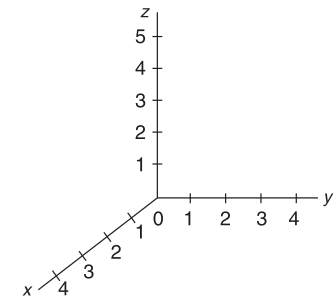
\includegraphics[width=0.5\linewidth]{img/coord_system.png}
    \caption{The Cartesian coordinate system.}
\end{figure}

We choose to represent points in space as three-dimensional \textit{position} vectors in this coordinate system of the form $ \bm{r} = (x, y, z)$ (or, alternatively, $ \bm{r} = x \ihat + y \jhat + z \khat$).

\begin{definition}
    A \textbf{position vector} is represented as a 3d vector of the form 
    $ \bm{r} = x \ihat + y \jhat + z \khat$
\end{definition}


Note that position vectors are dependent on a particular choice of coordinate system because they represent the vector from the origin of the coordinate system to the point of interest. Two or more position vectors can describe the same point in space. 

\indent Now we can define the difference, or \textbf{displacement}, between two vectors: 

\begin{definition}
    The \textit{displacement} between two vectors $ \vect{r_1} = x_1 \ihat + y_1 \jhat + z_1 \khat $ and $\vect{r_2} = x_2 \ihat + y_2 \jhat + z_2 \khat $ is the vector 

    $$ \svect{s} = \vect{r_1 r_2} = \vect{r_2} - \vect{r_1} = (x_2 - x_1) \ihat + (y_2 - y_1) \jhat + (z_2 - z_1) \khat$$
\end{definition}


\begin{figure}[H]
    \centering
    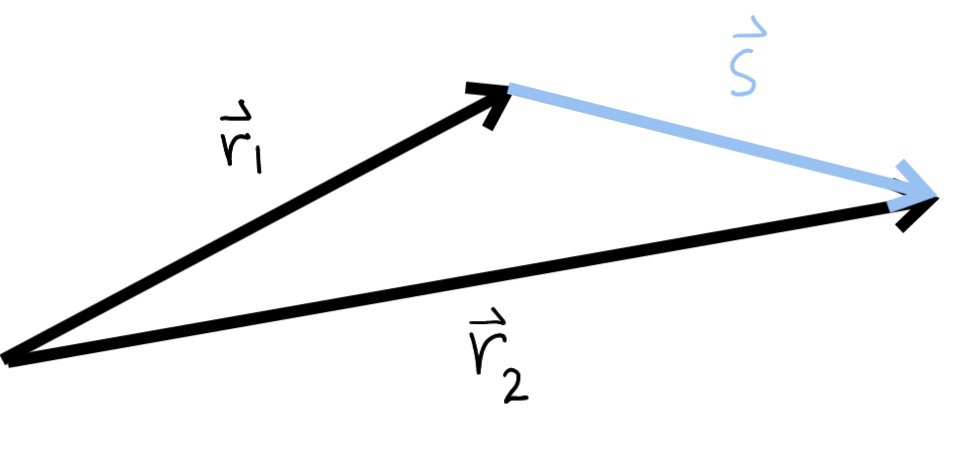
\includegraphics[width=0.3\linewidth]{img/image.png}
    \caption{A graphical representation of the displacement vector $\svect{s}$. }
    \label{fig:displacement_fig}
\end{figure}


Note that here, $r_1$ is the initial position and $r_2$ is the final position. Crucially, however, $\svect{s}$ does not depend directly on these positions but only their relative difference. 
Consider the scenario described by Figure \ref{ind}. 
\begin{figure}[H]
    \centering
    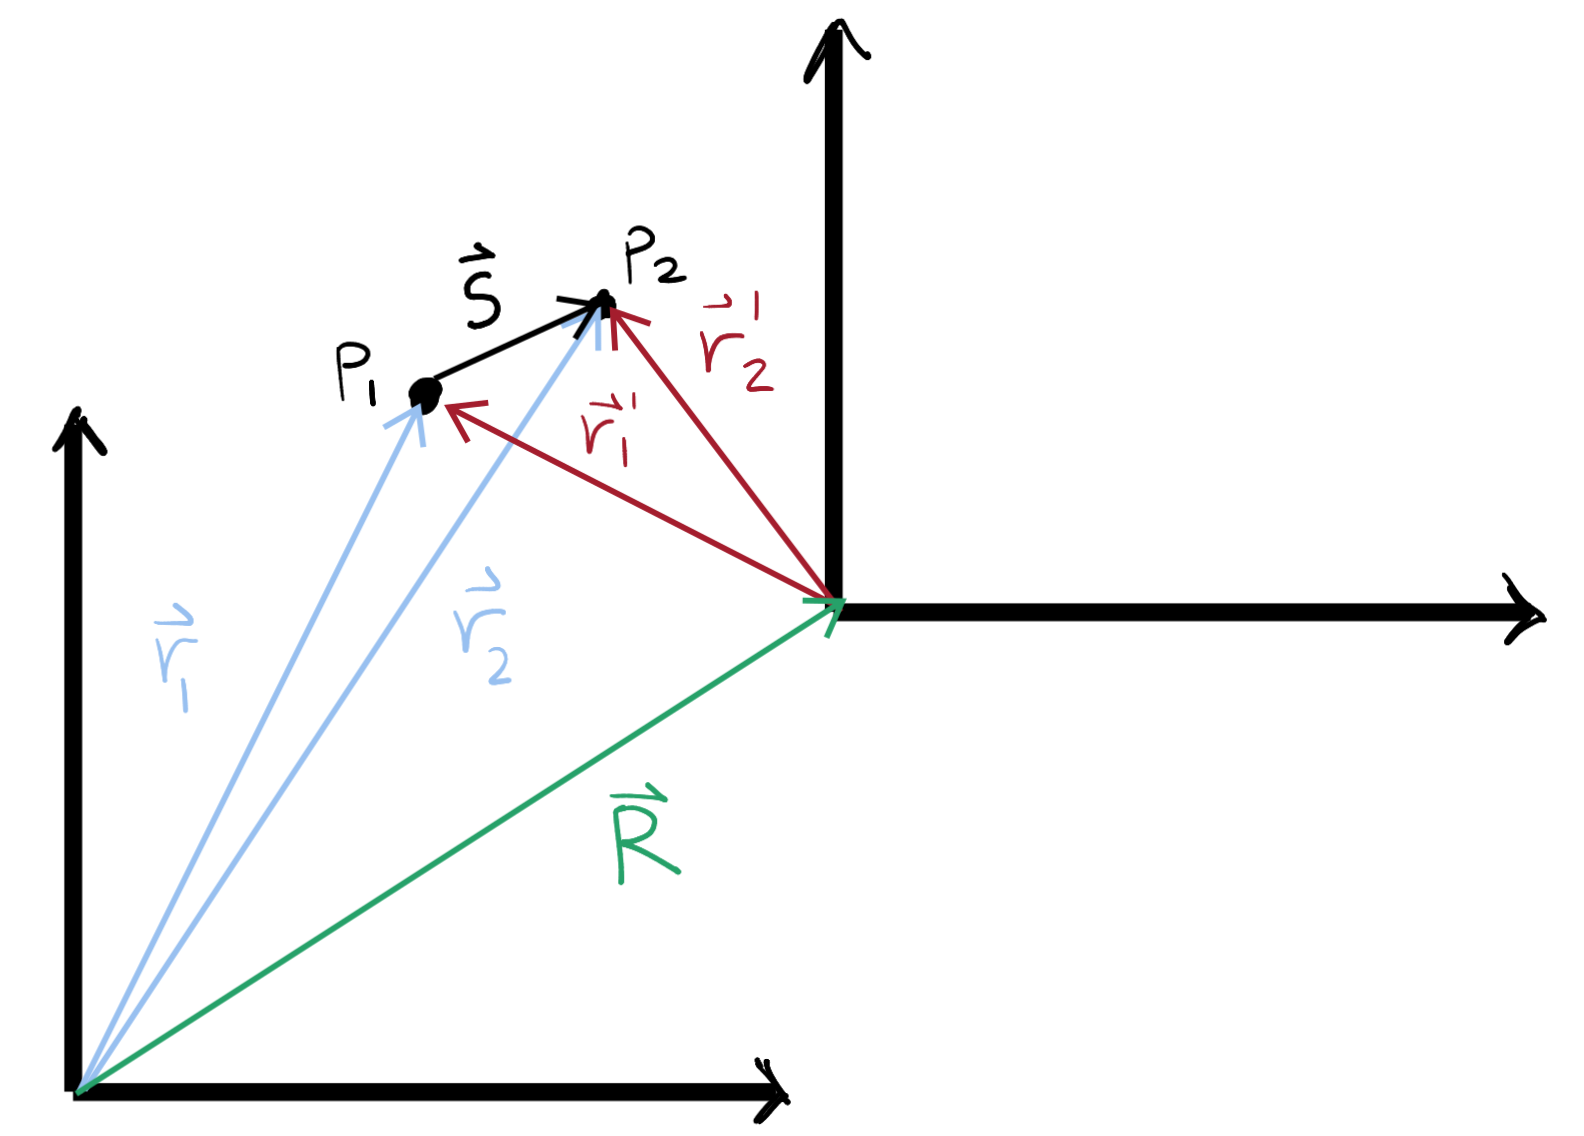
\includegraphics[width=0.5\linewidth]{img/coord_ref.png}
    \caption{A proof that displacement vectors are independent of a coordinate system.}
    \label{ind}
\end{figure}

In this figure, let $\vect{r_1}$ and $\vect{r_2}$ be the position vectors of points $P_1$ and $P_2$ with respect to the leftmost coordinate system, and let $\vect{r_1}'$ and $\vect{r_2}'$ be the position vectors of the same points with respect to the rightmost coordinate system. Additionally, let $\vect{R}$ be the vector connecting the origins of the two coordinate systems. Finally, let $\vect{s}$ be the displacement vector from $\vect{r_1}$ to  $\vect{r_2}$, and $\vect{s}'$ as the displacement vector from $\vect{r_1}'$ to $\vect{r_2}'$. We must show that $\vect{s} = \vect{s}'$. Notice that, from Figure \ref{ind}, it is immediately apparent that $\vect{r_1} = \vect{R} + \vect{r_1}'$ and $\vect{r_2} = \vect{R} + \vect{r_2}'$. Thus, from the above definitions it follows that 

\begin{align*}
\vect{s} & = \vect{r_2} - \vect{r_1} \\
            & = (\vect{R} + \vect{r_2}') - (\vect{R} + \vect{r_1}') \\
        & = \vect{r_2}' - \vect{r_1}'\\
        & = \vect{s_1}'\\
\end{align*}
Therefore, $\svect{s}$ is independent of any particular coordinate system. 

\section{Velocity and Acceleration}

Recall that in one dimension, the average velocity of a particle between two instances in time $\it{t_1}$ and $\it{t_2}$  can be written as 

$$ \bar{v} = \frac{x(t_2) - x(t_1)}{t_2 - t_1} $$

Taking the limit, we find that the \textbf{instantaneous velocity} can be defined as

\begin{definition}[One-Dimensional Instantaneous Velocity]

    $$ v(t) = \lim_{\Delta t \rightarrow 0}{\frac{x(t + \Delta t) - x(t)}{\Delta t}} = \frac{dx}{dt} = \dot{x}$$
    
\end{definition}

Similarly, for one-dimensional acceleration, the \textbf{instantaneous acceleration} is 

\begin{definition}[One-Dimensional Acceleration]
    $$ a(t) = \frac{dv}{dt} = \frac{d^2 x}{dt^2} = \dot{v} = \ddot{x}$$
\end{definition}

We can easily extend these definition to multiple dimensions using vectors. 

\section{Motion in Several Dimensions}

Consider a particle in a three-dimensional coordinate system whose position $\vect{r} = x(t) \ihat + y(t) \jhat + z(t) \khat $ varies as a function of time. Suppose that, in a brief time interval $\Delta t$ after a time $t$, the vector $\vect{r}$ changes by a displacement $\vect{\Delta r}$. Thus, we can define the the average velocity vector $\vect{\bar{v}}$ to be 

$$ \vect{\bar{v}} =  \frac{\vect{\Delta r}}{\Delta t} = \frac{\vect{r}(t + \Delta t) - \vect{r}(t)}{\Delta t}$$

Expanding the above expression component-wise we see that

$$  \frac{\vect{\Delta r}}{\Delta t} =
\frac{x(t+\Delta t) - x(t)}{\Delta t} \ihat +  \\
\frac{y(t+\Delta t) - y(t)}{\Delta t} \jhat + \\ 
\frac{z(t+\Delta t) - z(t)}{\Delta t} \khat
$$

Taking the limit as $\Delta t \rightarrow 0$ yields

\begin{definition}[Instantaneous Velocity]
    
$$ \vect{v} =  \frac{d\svect{r}}{dt} = \frac{dx}{dt} \ihat + \frac{dy}{dt} \jhat + \frac{dz}{dt} \khat $$
\end{definition}


Note that this step only works because the basis vectors $\ihat$, $\jhat$, and $\khat$ are independent of time, so they can be treated as constants. This is not true for other coordinate systems, such as a polar coordinate system. We can, similar to before, define the instantaneous acceleration as the time derivative of the above expression: 


\begin{definition}[Instantaneous Acceleration]
    \label{def:instacc}
    $$
        \vect{a} =  \frac{d\svect{v}}{dt} = \frac{d^2\vect{x}}{dt^2} 
    $$

\end{definition}

When visualizing the velocity vector $\vect{v}(t)$, it is helpful to note that the velocity vector is always tangent to the trajectory of the particle. This is because, for small $\Delta t$, 

\begin{equation}
\label{eq:parallel}
\frac{\vect{\Delta r}}{\Delta t} \approx \frac{d\svect{r}}{d t} = \vect{v}(t) \implies \vect{\Delta r} \approx \vect{v}(t) \Delta t
\end{equation}


\section{Formal Solutions to the Kinematic Equation}

Definition \ref{def:instacc} gives the three differential equations (one for each component) for the velocity 
in terms of the acceleration. A trivial integration gives

\begin{align}
    \vect{v}(t) = \vect{v}(t_0) + \int_{t_0}^{t} \vect{a}(t')dt'
    \label{eq:s}
\end{align}

Since position depends on velocity in a similar manner, a similar expression can be found
for the position in terms of velocity: 


\begin{align}
    \vect{r}(t) = \vect{r}(t_0) + \int_{t_0}^{t} \vect{v}(t')dt'
    \label{eq:t} 
\end{align}

Suppose that $\vect{a}$ is constant and $t_0 = 0$, then Eq. \ref{eq:s} and Eq. \ref{eq:t} become 

\begin{align*}
    \vect{v}(t) &= \vect{v_0} + \vect{a}t \\ 
    \implies \vect{r}(t) &= \vect{r_0} + \int_{0}^{t} (\vect{v_0} + \vect{a}t') dt'\\ 
                         &= \vect{r_0} + \vect{v_0}t + \frac{1}{2}\vect{a}t^2
\end{align*}

\begin{formula}[Kinematic Solution with Uniform Acceleration]
    For \textbf{uniform acceleration}, the solution to the kinematic 
    equations for position in terms of the initial conditions, and the acceleration is
    \[
        \vect{r}(t) = \vect{r_0} + \vect{v_0}t + \frac{1}{2}\vect{a}t^2
    \]
\end{formula}

\section{Rotating Vectors and Acceleration}

Unlike the scalar derivative, the derivative of a vector can cause
a vector to change either direction, magnitude, or both. 

\begin{figure}[H]
    \begin{center}
        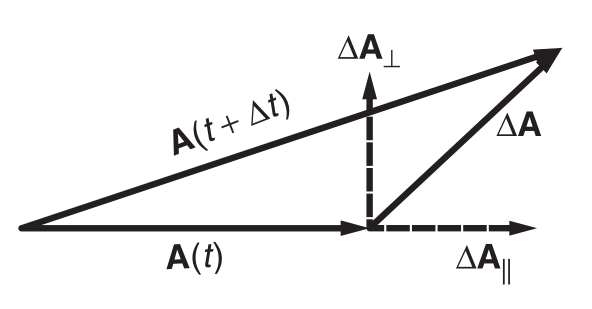
\includegraphics[width=0.5\textwidth]{img/rotvec.png}
    \end{center}
    \caption{}
    \label{fig:change}
\end{figure}

In Fig. \ref{fig:change}, a vector $\vect{A}$ changes by an amount
$\vect{\Delta A}$ over a small period of time $\Delta t$. $\vect{\Delta A}$ is 
resolved into two components, $\vect{\Delta A_\perp}$ and $\vect{\Delta A_\parallel}$. 
Consider how each of these components change $\vect{A}$ as $\Delta A \rightarrow 0$. 
The magnitude of $\vect{A}$ plus the perpendicular component is $\norm{\vect{A} +
\vect{\Delta A_{\perp}}} = \sqrt{A^2 + \Delta A_{\perp}^2 } \approx A$ for small $\Delta A_{\perp}$. 
Thus, the perpendicular component does not change the magnitude of $A$, it only rotates it. The parallel
component has no perpendicular component and thus only changes the magnitude of $A$. Recall that, by Eq. \ref{eq:parallel}, 
the velocity vector $\frac{d\vect{A}}{dt}$ is always parallel to the trajectory $\vect{\Delta A}$. Thus, if 
$\frac{d\vect{A}}{dt}$  is entirely perpendicular to $\vect{A}$ for all time, then 
$\vect{A}$ merely rotates and never changes its magnitude. \\ 

\begin{fact}
    
    For any time-varying vector $\vect{r}(t)$ with velocity $\vect{v}(t)$, if
    $\vect{r} \cdot \vect{v} = 0$ then the vector $\vect{r}$ undergoes only rotation for all time. 

    
\end{fact}

We can use this intuition to develop a useful expression for $\frac{d\vect{A}}{dt}$. Consider once again 
a time-varying vector $\vect{A}(t)$ such that $\vect{\Delta A} = \vect{\Delta A_{\parallel}} + \vect{\Delta A_{\perp}}$. 
Let $\Delta \theta$ be the angle between $\vect{A}(t)$ and $\vect{A}(t + \Delta t)$. Using the above results, 
for small $\Delta \theta$ we can write

\begin{align*}
    \Delta A_{\perp} &\approx A \Delta \theta \\
    \Delta A_{\parallel} &\approx \Delta A
\end{align*}

Thus, by taking the derivative we have 

\begin{align}
    \frac{dA_{\perp}}{dt} &= A \frac{d\theta}{dt} = A\omega \\
    \frac{dA_{\parallel}}{dt} &= \frac{dA}{dt}
\end{align}

If $\vect{A}(t)$ is only rotating, then $\frac{dA_{\parallel}}{dt} = 0$ and
$\frac{dA}{dt} = \frac{dA_{\perp}}{dt} = A\omega$. In the language of position and velocity, 

\[
    \dot{r}(t) = v(t) = r\omega 
\]



\section{Motion in Polar Coordinates}

\begin{figure}[H]
    \begin{center}
        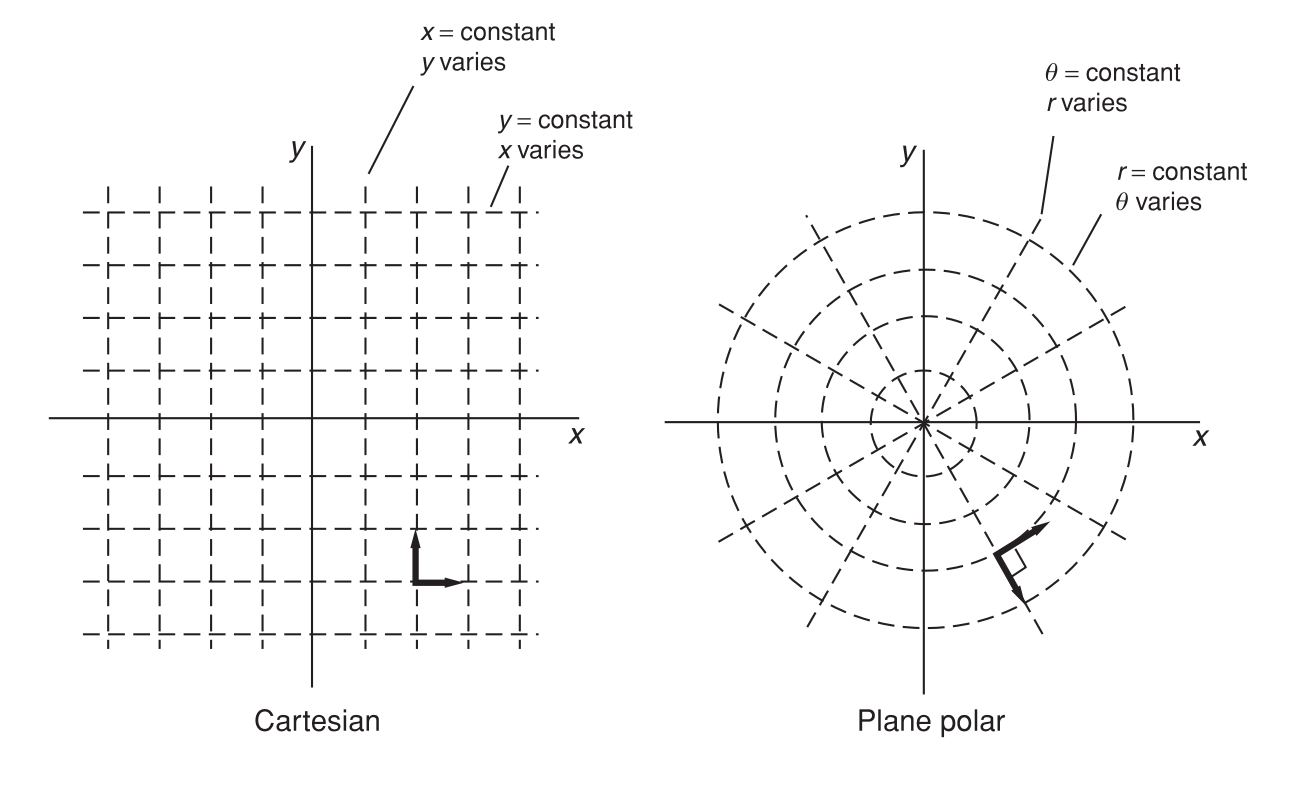
\includegraphics[width=0.5\textwidth]{img/polar.png}
    \end{center}
    \caption{A graphical representation of the polar coordinate system. }
    \label{fig:polar}
\end{figure}

In a \emph{polar} coordinate system, each point in space is represented 
as a tuple $(r, \theta)$ where $r$ is the distance from the origin and 
$\theta$ is the angle between $\vect{r}$ and the x-axis. To transfer between
Cartesian and polar points, we can use the following relations: 

\begin{align*}
    r &= \sqrt{x^2 + y^2}\\
    \tan(\theta) &= \frac{y}{x} \\
    x &= r\cos(\theta) \\
    y &= r\sin(\theta) 
\end{align*}

In a polar coordinate system, we introduce two new unit vectors, $\rhat$ and $\tthat$.
As in Figure \ref{fig:polar}, $\rhat$ points in the direction of increasing distance
from the origin while $\tthat$ points in the direction of increasing $\theta$. The figure below
illustrates the following relations between the unit vectors of the two coordinate systems:



\begin{figure}[H]
    \begin{center}
        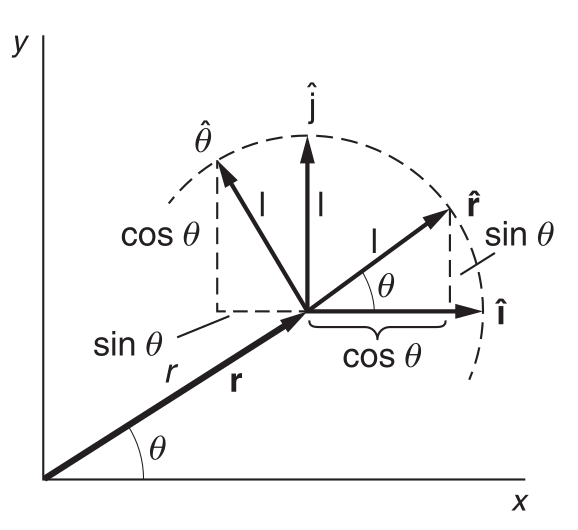
\includegraphics[width=0.4\textwidth]{img/rtheta.png}
    \end{center}
    \caption{}\label{fig:}
\end{figure}

\begin{definition}[Unit vectors in polar coordinates]
    \begin{align*}
        \rhat &= \cos(\theta)\ihat + \sin(\theta)\jhat \\
        \tthat &= -\sin(\theta)\ihat + \cos(\theta)\jhat
    \end{align*}

    Thus a position vector in polar coordinates is of the form 

    \[
        \vect{r} = r\rhat(\theta)
        \]

    Where $r$ is a function of time.
    
\end{definition}

It is important that $\rhat \cdot \tthat = 0$ to have an orthogonal basis
for the coordinate system. We will now establish two useful results, the 
derivatives of $\rhat$ and $\tthat$. These will be used to find expressions
for the velocity and acceleration in polar coordinates. 


\begin{align*}
    \dv{\rhat}{t} &= -\sin(\theta) \dot{\theta} \ihat + \cos(\theta) \dot{\theta} \jhat \\
                  &= \dot{\theta}\tthat 
\end{align*}


\begin{align*}
    \dv{\tthat}{t} &= -\cos(\theta) \dot{\theta} \ihat - \sin(\theta) \dot{\theta} \jhat \\
                     &= -\dot{\theta}\rhat
\end{align*}


To find the velocity, using the above expressions,

\begin{align*}
    \vect{v} = \dv{\vect{r}}{t} &= \dv{t}(r\rhat) = \dot{r}\rhat + r\dot{\theta}\tthat
\end{align*}

A similar derivation for acceleration in polar coordinates yields

\begin{align*}
    \vect{a} = \dv{\vect{v}}{t} &= \ddot{r}\rhat + \dot{r}\dot{\theta}\tthat + \dot{r}\dot{\theta}\tthat + r\ddot{\theta}\tthat + -r\dot{\theta}^2\rhat \\
            &= (\ddot{r} - r\dot{\theta}^2)\rhat + (2\dot{r}\dot{\theta} + r\ddot{\theta})\tthat
\end{align*}

In summary, 

\begin{definition}[Polar Acceleration and Velocity]

    \label{def:test}
    \begin{align*}
        \vect{v} &= \dot{r}\rhat + r\dot{\theta}\tthat \\
        \vect{a} &= (\ddot{r} - r\dot{\theta}^2)\rhat + (2\dot{r}\dot{\theta} + r\ddot{\theta})\tthat
    \end{align*}
\end{definition}

\begin{figure}[H]
    \begin{center}
        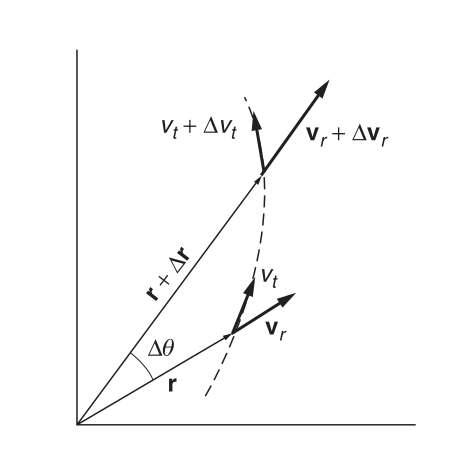
\includegraphics[width=0.4\textwidth]{img/polaraccel.png}
    \end{center}
    \caption{A geometric view of acceleration in polar coordinates.}\label{fig:polaraccel}
\end{figure}

(FIX THIS chapter, USE VTHETA INSTEAD OF THE CRAP KK USES) Each of the terms in these equations has a physical interpretation. 
The $\dot{r}\rhat$ and $\ddot{r}\rhat$ terms are called the \textbf{tangential
velocity} and \textbf{acceleration}, respectively. These terms are related to 
changes in magnitude speed and position along the radial direction. Additionally, 
the $r\dot{\theta}$ and $r\dot{\theta}^2$ terms called the \textbf{centripetal}
acceleration and velocity and are related to a change in the direction of the position 
and speed. Finally, $2\dot{r}\dot{\theta}$ is the \textbf{Coriolis acceleration} while
$r\ddot{\theta}$ is the acceleration due to a change in the tangential component of 
the velocity. Figure \ref{fig:polaraccel} illustrates the radial and tangential components
of the velocity vector, which can be used to derive \ref{def:test} from geometric principles, 
as we did before with rotating vectors. 


\chapter{Newton's Laws of Motion}

\section{Newton's First Law}

To describe motion it is essential to have a coordinate system. An \textbf{inertial} coordinate system is one which is moving at a constant velocity; not accelerating. 
Luckily, it is always possible to find such a coordinate system, in which isolated bodies move uniformly. Newton's first law of motion 
is merely the assertion that

\begin{fact}[Newton's First Law of Motion]
    Inertial coordinate systems, which are coordinate systems that move at constant velocity, exist.  
\end{fact}

\section{Mass, Force, and Newton's Second Law}

Consider pulling a cart on a frictionless track with a rubber band stretched to a constant length. The cart accelerates at a constant rate; a heavier cart accelerates less for the same applied force. This motivates an operational definition: if $m_1$ is one unit of mass, then a second cart with acceleration $a_2$ under the same force has mass

\[
    m_2 \defeq m_1 \frac{a_1}{a_2}
\]

Extending this reasoning, two rubber bands produce twice the acceleration, and pulling in opposite directions produces no acceleration, confirming that forces add as vectors. With $F = 1$ unit of force acting on $m$ units of mass producing acceleration $a = F/m$, we can write Newton's Second Law:

\begin{fact}[Newton's Second Law]
    In an inertial system, 

    \[
        \vect{F} = m\vect{a} 
    \]

    where $[F] = \text{kg}\frac{\text{m}}{\text{s}^2}$
\end{fact}

Forces arise from physical \textit{interactions} between systems; accelerations are merely the consequence of that. 
Thus, if something is accelerating, it is not a guarantee that there is a force acting upon it. 

\section{Newton's Third Law of Motion}

\begin{fact}[Newton's Third Law]

    Suppose there are two bodies, $a$ and $b$. If body $b$ exerts  a force on $a$, $\vect{F_{ba}}$, then there is an equal and opposite
    acting on $b$, $\vect{F_{ab}} = \vect{-F_{ba}}$

\end{fact}

The significance of this law is that there is never a force without it's corresponding pair in another system, which allows
us to check if an acceleration is due to a force or something else. 

\section{Fictitious Forces}

While the surface of the Earth provides a reasonably good approximation of an inertial system, it is not exactly one
due to it's rotation. This results in so-called \textit{fictitious forces}, which appear to not come from any outside system. 
For systems moving with a constant acceleration vector, there is an easy way to account for these forces. Consider the following:


\begin{figure}[H]
    \begin{center}
        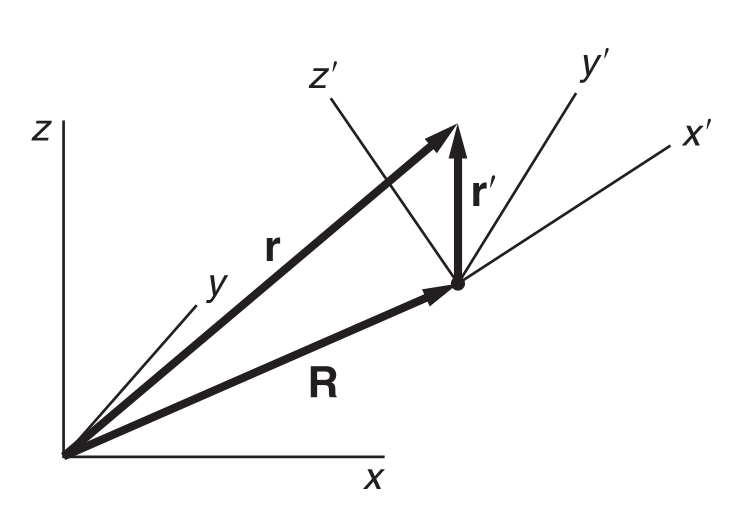
\includegraphics[width=0.5\textwidth]{img/ficforce.png}
    \end{center}
    \caption{Position vectors of an inertial and non-inertial coordinate systems.}\label{fig:fictforce}
\end{figure}

Figure \ref{fig:fictforce} shows two coordinate systems, $(x, y, z)$ and $(x', y', z')$. The former is inertial, 
while the latter moves with constant acceleration $\vect{R}$. The vector $\vect{r}$ shows the position of an accelerating 
body with respect to the inertial coordinate system and the vector $\vect{r'}$ shows the position with respect 
to the inertial coordinate system. Using vector addition, we see from the diagram that

\[
    \vect{r} = \vect{r'} + \vect{R} 
\]

Differentiating twice with respect to time, 

\[
    \vect{\ddot{r}} = \vect{\ddot{r'}} + \vect{\ddot{R}}
\]

Multiplying by the mass of the particle, 
\[
    m\vect{\ddot{r}} = m\vect{\ddot{r'}} + m\vect{\ddot{R}} \\
\]
Thus by Newton's Second Law, 
\[    
    \vect{F}_\text{true} = \vect{F}_\text{apparent} + m\vect{\ddot{R}} 
\]

Since we are interested in the force measured in the non-inertial frame, we can write


\[    
    \vect{F}_\text{apparent} = \vect{F}_\text{true} + \vect{F}_\text{fictitious} 
\]

where $\vect{F}_\text{fictitious} = -m\vect{\ddot{R}}$.

\section{Applying Newton's Laws}

The following procedure can be used to approach problems involving Newton's Laws: 

\begin{enumerate}
    \item \textbf{Isolate the masses. } Divide each system into collections of masses, each of which can be 
        treated as a particle. 
    \item \textbf{Draw a force diagram for each mass. } Represent each body by a point or symbol, and draw all the forces
        acting \textit{on} each body as an arrow vector starting from the point/symbol. Even if you assume a force is in the wrong up/down 
        direction, it will simply come out to having a negative sign in the final answer.
    \item \textbf{Show a coordinate system on the force diagram. } Choose convenient directions for the coordinate axes. 
    \item \textbf{Write down the equations of motion. } The equations will usually be of the form $F_1 + F_2 + \dots = ma$ For each component of the vectors there should be a separate equation.
    \item \textbf{Write down the constraint equations. } These equations will come from geometric considerations, such as considering the relationship between the lengths or accelerations
        of the bodies in the system. The total number of equations of motion and constraint equations should equal the number of unknowns in the problem. 
\end{enumerate}

\chapter{Forces and Equations of Motion}

\section{Gravitational Forces, Acceleration due to Gravity, and Weight}

This chapter will introduce new kinds of forces, which are primarily derived from electrostatic and gravitational interactions. 
The first of these forces is the all-too familiar Law of Gravitation: 

\begin{fact}[Newton's Law of Gravitation]
    Consider two particles with masses $M_a$ and $M_b$ separated by a distance $r$. Let $\vect{F_{ba}}$ be the gravitational force exerted by particle
    $b$ on particle $a$. Then 
    \[
        \vect{F_{ba}} = -\frac{G M_a M_b}{r^2}\rhat  
    \]
    Where $\vect{r} = \vect{r_a r_b}$ and $G$ is the \textbf{Gravitational Constant}. 
\end{fact}

A useful corrollary of this law is that

\begin{fact}
    The gravitational force at any point inside a spherical shell of mass is 0. Additionally, outside of the spherical shell, 
    the shell produces a net gravitational force which is the same as if all its mass is produced at its center. More formally, 
    suppose there is a particle of mass m and a uniform thin spherical shell of mass $M$ and radius $R$. Then 

    \[
        \vect{F} = \begin{cases}
            0 & r < R \\
            -\frac{G M m}{r^2}\rhat & r > R \\  
        \end{cases} 
    \]

    where $\vect{r}$ is the vector pointing \textit{from} the center of the shell \textit{to} $m$.
\end{fact}

A rigorous proof of this fact will not be given here, but the intuitive idea is that the proportion of the shell's surface area containing mass a particle
"sees" increases with the distance from the surface squared, but by the above equation, the gravitational force produced by a given part of that 
surface area decreases as the distance squared. Thus, the forces from each segment of the surface cancel out. 
\newpage

% ============================================================
% Continuation from ch3 (Forces, Shell Theorem)
% Pages 12–38: Atwood machine, polar coordinates kinematics,
%   friction, Newton's laws, spring force, pendulum, adding
%   springs, viscosity, and recitation problems.
% ============================================================

\section{Inclined Plane (continued)}

\begin{figure}[H]
\begin{center}
\begin{tikzpicture}[scale=1.1, >=Stealth]
  % Inclined plane triangle
  \draw[thick] (0,0) -- (4,0) -- (4,2.3) -- cycle;
  \node at (0.7,0.18) {$\theta$};
  \draw (0.55,0) arc[start angle=0, end angle=30, radius=0.55];
  % Block
  \def\bx{1.6}\def\by{0.92}
  \begin{scope}[rotate around={30:(\bx,\by)}]
    \fill[gray!30] (\bx-0.3,\by-0.3) rectangle (\bx+0.3,\by+0.3);
    \draw[thick] (\bx-0.3,\by-0.3) rectangle (\bx+0.3,\by+0.3);
  \end{scope}
  % Weight arrow (downward)
  \draw[->,thick,blue] (1.6,0.92) -- (1.6,-0.5) node[below]{$\vect{w}=m\vect{g}$};
  % Normal arrow (perpendicular to slope)
  \draw[->,thick,red] (1.6,0.92) -- ++(150:1.1) node[above left]{$\vect{N}$};
  % Acceleration along slope
  \draw[->,thick,ForestGreen] (1.6,0.92) -- ++(30:1.1) node[right]{$\vect{a}$};
\end{tikzpicture}
\end{center}
\caption{Block on a frictionless inclined plane at angle $\theta$; normal force $\vect{N}$ perpendicular to surface, weight $\vect{w} = m\vect{g}$ downward.}
\label{fig:inclined_plane}
\end{figure}

Newton's second law $\vect{N} + \vect{w} = m\vect{a}$, projected onto axes along and perpendicular to the slope:

\begin{align*}
x&: \quad w\sin\theta = ma \implies mg\sin\theta = ma \implies a = g\sin\theta \\
y&: \quad N - w\cos\theta = 0
\end{align*}

\textbf{Limiting cases:} $\theta = 0$ (flat, $a=0$) \checkmark \quad $\theta = \tfrac{\pi}{2}$ (free fall, $a=g$) \checkmark

% ============================================================
\section{Atwood Machine}
% ============================================================

\begin{figure}[H]
\begin{center}
\begin{tikzpicture}[scale=0.9, >=Stealth]
  % Pulley support and axle
  \draw[thick] (-0.1,3.2) -- (0.1,3.2);
  \draw[thick] (0,3.2) -- (0,2.8);
  % Pulley circle
  \draw[thick] (0,2.5) circle[radius=0.3];
  \fill[gray!40] (0,2.5) circle[radius=0.08];
  % Left rope and mass m1
  \draw[thick] (-0.3,2.5) -- (-0.3,1.2);
  \fill[gray!50] (-0.55,0.8) rectangle (-0.05,1.2);
  \draw[thick] (-0.55,0.8) rectangle (-0.05,1.2);
  \node at (-0.3,1.0) {$m_1$};
  \draw[->,thick,blue] (-0.3,0.8) -- (-0.3,0.1) node[below]{$w_1$};
  \draw[->,thick,red] (-0.3,1.2) -- (-0.3,1.9) node[right]{$T_1$};
  % Right rope and mass m2
  \draw[thick] (0.3,2.5) -- (0.3,0.7);
  \fill[gray!50] (0.05,0.3) rectangle (0.55,0.7);
  \draw[thick] (0.05,0.3) rectangle (0.55,0.7);
  \node at (0.3,0.5) {$m_2$};
  \draw[->,thick,blue] (0.3,0.3) -- (0.3,-0.3) node[below]{$w_2$};
  \draw[->,thick,red] (0.3,0.7) -- (0.3,1.4) node[right]{$T_2$};
  % Ceiling
  \fill[pattern=north east lines] (-0.5,3.2) rectangle (0.5,3.4);
  \draw[thick] (-0.5,3.2) -- (0.5,3.2);
\end{tikzpicture}
\end{center}
\caption{Atwood machine: two masses $m_1$ and $m_2$ connected by an inextensible rope over a pulley of radius $R$. Tensions $T_1$, $T_2$ act upward on each mass; weights $w_1$, $w_2$ act downward.}
\label{fig:atwood}
\end{figure}

\begin{example}[Atwood Machine]
Two masses $m_1$ and $m_2$ hang from either end of a rope over a fixed pulley. Find the acceleration.

\textbf{System \{1\}:} tension $T_1$ upward, weight $w_1 = m_1 g$ downward.
\[
\vect{T}_1 + \vect{w}_1 = m_1 \vect{a}_1 \implies T_1 - m_1 g = m_1 \ddot{y}_1
\]

\textbf{System \{2\}:} tension $T_2$ upward, weight $w_2 = m_2 g$ downward.
\[
T_2 - m_2 g = m_2 \ddot{y}_2
\]

\textbf{Constraint} --- length of rope is constant $= \ell$:
\[
\ell = y_p - y_1 + y_p - y_2 + \pi R
\]
Differentiating twice:
\[
\dv{\ell}{t} = 0 = -\dot{y}_1 - \dot{y}_2 \implies 0 = -\dot{y}_1 - \dot{y}_2
\]

The tension of the rope should balance unless the rope is stretching, so $T_1 = T_2 \equiv T$.

\textbf{Putting everything together:}
\begin{align*}
T - m_1 g &= m_1 \ddot{y}_1 \\
T - m_2 g &= m_2 \ddot{y}_2
\end{align*}

Using the constraint $\ddot{y}_2 = -\ddot{y}_1$, subtract the two equations:
\begin{align*}
(T - m_1 g) - (T - m_2 g) &= m_1 \ddot{y}_1 + m_2 \ddot{y}_1 \\
(-m_1 + m_2)g &= (m_1 + m_2)\ddot{y}_1
\end{align*}

\begin{formula}[Atwood Machine Acceleration]
\[
\ddot{y}_1 = \frac{(-m_1 + m_2)\,g}{m_1 + m_2} = \frac{(m_2 - m_1)\,g}{m_1 + m_2}
\]
\end{formula}

\textbf{Check:} if $m_1 \gg m_2 \Rightarrow \ddot{y}_1 = -g$ (mass 1 falls freely). \checkmark
\end{example}

% ============================================================
\section{Polar Coordinates Example}
% ============================================================

\begin{example}[Rotating Table with Hanging Mass]
A object $A$ rotates at angular speed $\omega_0$ at radius $r_0$ on a frictionless horizontal table. It is connected through a hole in the table by a string to a hanging mass $B$. What is the acceleration of $A$ after $B$ is released?

\begin{figure}[H]\centering
\caption{Mass $A$ on a rotating table connected via a string through the table centre to hanging mass $B$. The string length $L = r + y_B = \text{const}$.}
\end{figure}

\textbf{System \{A\}:} Only horizontal tension $T$ acts (normal $N$ and weight $w_A$ cancel vertically).
\[
\vect{T} = m_A \vect{a}_A, \qquad
\vect{a}_A = (\ddot{r} - r\dot{\theta}^2)\,\rhat + (r\ddot{\theta} + 2\dot{r}\dot{\theta})\,\tthat
\]

Projecting:
\begin{align*}
\rhat&: \quad -T = m_A(\ddot{r} - r\dot{\theta}^2) \tag{1} \\
\tthat&: \quad 0 = m_A(r\ddot{\theta} + 2\dot{r}\dot{\theta}) \tag{2}
\end{align*}

\textbf{System \{B\}:} weight $m_B g$ downward, tension $T$ upward.
\[
m_B g - T = m_B \ddot{y}_B \tag{3}
\]

\textbf{Constraint:} $L = r + y_B = \text{const}$, so differentiating:
\[
\dot{r} = -\dot{y}_B \implies \ddot{r} = -\ddot{y}_B \tag{4}
\]

\textbf{Initial conditions:} $r = r_0$, $\dot{\theta} = \omega_0$.

From (1): $T = -m_A(\ddot{r} - r\dot{\theta}^2) = m_A(r\dot{\theta}^2 - \ddot{r})$.

Substituting into (3) with $\ddot{y}_B = -\ddot{r}$:
\begin{align*}
m_B g - m_A(r\dot{\theta}^2 - \ddot{r}) &= m_B(-\ddot{r}) \\
m_B g + m_A \ddot{r} - m_A r\dot{\theta}^2 &= -m_B \ddot{r} \\
m_B g + m_B \ddot{r} + m_A \ddot{r} &= m_A r\dot{\theta}^2 \\
\ddot{r}(m_A + m_B) &= m_A r\dot{\theta}^2 - m_B g
\end{align*}

\begin{formula}[Polar Constraint System]
\[
\ddot{r} = \frac{m_A r\dot{\theta}^2 - m_B g}{m_A + m_B}
\]
\end{formula}
\end{example}

% ============================================================
\chapter{Forces}
% ============================================================

\section{Friction}

\begin{definition}[Friction]
Friction arises when the surface of one body moves (or tends to move) across another. It:
\begin{itemize}
  \item opposes motion,
  \item is independent of the area of the object,
  \item acts proportional to the normal force $N$.
\end{itemize}
\[
f = \mu N \qquad (\mu \text{ a unitless constant})
\]
\end{definition}

\subsection{Types of Friction}

There are two coefficients: $\mu_{\text{static}}$ and $\mu_{\text{kinetic}}$.

\begin{fact}[Static Friction]
Bodies are \emph{not} in relative motion:
\[
0 \le f_s \le \mu_s N
\]
Direction: opposes the motion the object \emph{would} have if it were moving.
\end{fact}

\begin{fact}[Kinetic Friction]
\[
f_k = \mu_k N
\]
Direction: opposite to the relative velocity.
\end{fact}

\textbf{Decision flowchart for friction:}
\begin{enumerate}
  \item Are the objects accelerating relative to each other?
    \begin{itemize}
      \item Yes $\Rightarrow f = \mu_k N$.
      \item No $\Rightarrow$ Are the objects just about to slip/not slip?
        \begin{itemize}
          \item Yes $\Rightarrow f = \mu_s N$.
          \item No $\Rightarrow$ don't assume anything about $f$; solve for it.
        \end{itemize}
    \end{itemize}
\end{enumerate}

\begin{example}[Block on Wedge with Friction]
A block of mass $m$ sits on a wedge at angle $\theta$. Forces: normal $N$, friction $f$, weight $mg$.

\begin{figure}[H]
\begin{center}
\begin{tikzpicture}[scale=1.0, >=Stealth]
  % Inclined wedge
  \draw[thick,fill=gray!10] (0,0) -- (3.5,0) -- (3.5,2.0) -- cycle;
  \node at (0.65,0.15) {$\theta$};
  \draw (0.55,0) arc[start angle=0, end angle=30, radius=0.55];
  % Block (rotated)
  \begin{scope}[rotate around={30:(1.5,0.86)}]
    \fill[gray!40] (1.2,0.6) rectangle (1.8,1.12);
    \draw[thick] (1.2,0.6) rectangle (1.8,1.12);
  \end{scope}
  \node at (1.65,0.9) {$m$};
  % Weight arrow
  \draw[->,thick,blue] (1.5,0.86) -- (1.5,-0.15) node[below]{$mg$};
  % Normal force (perpendicular to slope = direction 120 deg)
  \draw[->,thick,red] (1.5,0.86) -- ++(120:1.1) node[above]{$N$};
  % Friction force (up the slope = 30 deg direction)
  \draw[->,thick,ForestGreen] (1.5,0.86) -- ++(150:0.85) node[left]{$f$};
\end{tikzpicture}
\end{center}
\caption{Free-body diagram of block on inclined wedge at angle $\theta$: weight $mg$ downward, normal force $N$ perpendicular to surface, friction $f$ along the surface opposing motion.}
\label{fig:friction_wedge}
\end{figure}

\begin{align*}
x&: \quad mg\sin\theta - \mu F_N = m\ddot{x} \\
y&: \quad N - mg\cos\theta = 0 \implies N = mg\cos\theta
\end{align*}
\[
\therefore\quad \ddot{x} = g\sin\theta - \mu g\cos\theta
\]

\textbf{Maximum angle before sliding begins:}
\[
\theta_{\max} = \tan^{-1}(\mu)
\]
For different materials, the block starts sliding at different angles.
\end{example}


% ============================================================
\chapter{Dimensional Analysis and Order-of-Magnitude Estimates}
% ============================================================

\section{Dimensional Analysis}

\begin{definition}[Dimensional Analysis]
Shorthand solving using units alone. Used to check answers. \emph{NOT} to be confused with unit conversion.
\end{definition}

\begin{example}[Period of a Pendulum]
Relevant quantities: $\ell$ (length), $g$ (gravitational acceleration), $m$ (mass).
\[
[\ell] = L, \quad [g] = \frac{L}{T^2}, \quad [m] = M
\]

Assume $P = A\,\ell^x g^y m^z$. Then:
\[
T = A \cdot L^x \cdot \left(\frac{L}{T^2}\right)^y \cdot M^z = A\cdot L^{x+y} \cdot T^{-2y} \cdot M^z
\]

Matching exponents: $-2y = 1 \Rightarrow y = -\tfrac{1}{2}$; $x + y = 0 \Rightarrow x = \tfrac{1}{2}$; $z = 0$.

\[
\therefore\quad P = A\sqrt{\frac{\ell}{g}}
\]
\end{example}

\section{Order-of-Magnitude / Back-of-the-Envelope Estimates}

\begin{example}[Volume of Earth's Atmosphere]
\[
V_{\text{atmosphere}} \approx 4\pi R_\oplus^2 \cdot t
\]
where $t$ is the thickness of the atmosphere. Assume $t \approx 10^4\,\mathrm{m}$, $R_\oplus = 6\times 10^6\,\mathrm{m}$, and $t \ll R_\oplus$:
\[
\Rightarrow V \approx \boxed{4\times 10^{18}\,\mathrm{m}^3}
\]
\end{example}

\begin{example}[Terminal Velocity of a Raindrop]
Equation of motion with drag $F = -kv^2$:
\[
\dv{v}{t} = g - kv^2
\]
At terminal velocity $\dv{v}{t} = 0$:
\[
V_t \approx \sqrt{\frac{g}{k}}
\]
Dimensional check: $\left[\dv{v}{t}\right] = \dfrac{L}{T^2}$, $\dfrac{L}{T^2} - \left(\dfrac{1}{L}\right)\dfrac{L^2}{T^2}$ so $[k] = \dfrac{1}{L}$.

Order-of-magnitude estimate: $V_t \approx 5\,\mathrm{m/s}$.

What is $\kappa$?
\[
k = \frac{g}{V_t^2} \approx \frac{10\,\mathrm{m/s}^2}{(5\,\mathrm{m/s})^2} \approx 0.4\,\mathrm{m}^{-1}
\]
\end{example}

\section{Gravity (Newton's Law of Gravitation)}

\begin{figure}[H]\centering
\caption{Two masses $M_a$ and $M_b$ separated by distance $r$; gravitational force $\vect{F}_{ba}$ on $b$ from $a$ directed toward $a$, and $\vect{F}_{ab}$ directed toward $b$.}
\end{figure}

\begin{formula}[Newton's Law of Gravitation]
\[
\left|\vect{F}_{b/a}\right| = \frac{G m_a m_b}{r^2}
\]
Dimensions of $G$: $\dfrac{M \cdot L/T^2 \cdot L^2}{M^2} = \dfrac{L^3}{M \cdot T^2}$, i.e.\ $\mathrm{m}^3\,\mathrm{kg}^{-1}\,\mathrm{s}^{-2}$.
\end{formula}

Gravity is a \textbf{central} force, so:
\[
\vect{F}_{BA} = -\frac{GM_A M_B}{r^2}\,\rhat
\]

\subsection{Shell Theorem Results}

For a uniform spherical shell of mass $M$ and radius $R$:
\begin{align*}
r < R&: \quad \vect{F} = \vect{0} \\
r \ge R&: \quad \vect{F} = -\frac{GmM}{r^2}\,\rhat
\end{align*}

\subsection{Additional Notes on Gravity}

For acceleration due to gravity $g$, $\Delta g$ can be calculated as:
\[
\Delta g = g(R_e + h) - g(R_e) \approx h\,\dv{g}{r} = -\frac{2GM_e\,h}{R_e^3} = -2g\frac{h}{R_e}
\]

\textbf{Weight} at the surface of the Earth:
\[
W = -\frac{GM_e m}{R_e^2}\,\rhat = mg
\]

\section{Equivalence Principle}

\begin{fact}[Equivalence Principle]
Acceleration due to gravity is independent of mass.
\end{fact}

\section{Electrostatic Force}

\begin{formula}[Coulomb's Law]
\[
\vect{F}_{ba} = k\frac{q_1 q_2}{r^2}\,\hat{r}_{ba}, \qquad E = k\frac{q}{r^2}\,\rhat
\]
\end{formula}

\section{Phenomenological Forces}

\subsection{Contact Forces}

Forces transmitted between bodies by short-range interactions.

\subsection{Tension}

\begin{definition}[Tension]
Force due to a string's resistance to increasing length. You can imagine a chain of molecules that pull on each other as a string.

\begin{figure}[H]\centering
\caption{Each segment of the string transmits force $F'$ inward on both sides; applied force $F$ at one end. The tension is the same throughout a massless, inextensible string.}
\end{figure}
\end{definition}


% ============================================================
\chapter{Spring Force and Simple Harmonic Motion}
% ============================================================

\section{Hooke's Law}

\begin{formula}[Hooke's Law]
\[
\vect{F} = -k(\vect{x} - \vect{x}_0)
\]
where $x_0$ is the length of the spring at equilibrium.
\end{formula}

\begin{figure}[H]
\begin{center}
\begin{tikzpicture}[scale=1.0, >=Stealth]
  % Wall
  \fill[pattern=north east lines] (-0.2,-0.4) rectangle (0,0.4);
  \draw[thick] (0,-0.4) -- (0,0.4);
  % Spring (zigzag)
  \draw[thick, decorate, decoration={zigzag, segment length=6pt, amplitude=4pt}]
    (0,0) -- (2.5,0);
  % Mass block
  \fill[gray!40] (2.5,-0.3) rectangle (3.1,0.3);
  \draw[thick] (2.5,-0.3) rectangle (3.1,0.3);
  \node at (2.8,0) {$m$};
  % Equilibrium marker
  \draw[dashed] (2.8,-0.5) -- (2.8,-0.85);
  \node[below] at (2.8,-0.85) {$x_0$};
  % Spring force arrow
  \draw[->,thick,red] (3.1,0) -- (3.9,0) node[right]{$x$};
  \draw[->,thick,blue] (2.5,0) -- (1.7,0) node[left]{$F_s$};
  % Ground line
  \draw[thick] (-0.2,-0.4) -- (4.0,-0.4);
\end{tikzpicture}
\end{center}
\caption{Mass on a spring: equilibrium position $x_0$, displacement $x$ to the right, restoring spring force $F_s = -k(x-x_0)$ directed back toward equilibrium.}
\label{fig:spring_mass}
\end{figure}

Equation of motion (1D):
\[
\vect{F} = m\vect{a} \implies m\ddot{x} = -k(x - x_0)
\]

\subsection{Solving the Equation of Motion}

Introduce change of variables $\Delta x = x - x_0$, so $\Delta \ddot{x} = \ddot{x}$:
\[
\Delta\ddot{x} = -\frac{k}{m}\Delta x \qquad \textbf{(extremely important)}
\]

This is a second-order ODE, requiring 2 sets of initial conditions.

\textbf{Guess a solution and check:}
\[
y(t) = A\cos(\omega t + \phi_0)
\]
\[
\dot{y}(t) = -\omega A\sin(\omega t + \phi_0)
\]
\[
\ddot{y}(t) = -A\omega^2\cos(\omega t + \phi_0)
\]

Substituting:
\[
-A\omega^2\cos(\omega t + \phi_0) = -\frac{k}{m}A\cos(\omega t + \phi_0)
\]

\begin{formula}[Angular Frequency of SHM]
\[
\omega^2 = \frac{k}{m} \implies \omega = \sqrt{\frac{k}{m}}
\]
\end{formula}

\textbf{Interpretation of parameters:}
\begin{itemize}
  \item $A$: Amplitude — maximum distance it will travel.
  \item $\phi_0$: Phase — initial displacement; where did my system start at $t = 0$.
  \item $\omega$: Angular frequency — tells us about the period.
\end{itemize}

\begin{figure}[H]
\begin{center}
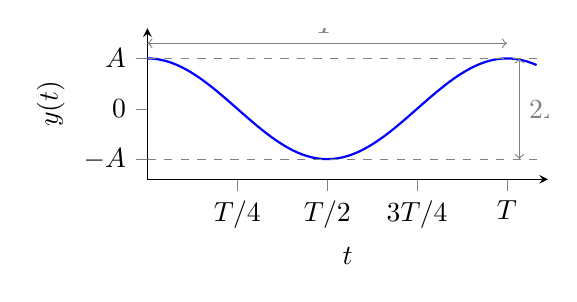
\begin{tikzpicture}
\begin{axis}[
  width=0.55\textwidth, height=3.5cm,
  xlabel={$t$}, ylabel={$y(t)$},
  xmin=0, xmax=7, ymin=-1.4, ymax=1.6,
  xtick={1.5708, 3.1416, 4.7124, 6.2832},
  xticklabels={$T/4$, $T/2$, $3T/4$, $T$},
  ytick={-1,0,1},
  yticklabels={$-A$, $0$, $A$},
  axis lines=left,
  tick align=outside,
  samples=200,
]
  \addplot[thick, blue, domain=0:6.8] {cos(deg(x))};
  % Amplitude annotations
  \draw[dashed, gray] (axis cs:0,1) -- (axis cs:6.8,1);
  \draw[dashed, gray] (axis cs:0,-1) -- (axis cs:6.8,-1);
  \draw[<->,gray] (axis cs:6.5,-1) -- (axis cs:6.5,1) node[midway,right]{$2A$};
  % Period brace
  \draw[<->,gray] (axis cs:0,1.3) -- (axis cs:6.2832,1.3) node[midway,above]{$T$};
\end{axis}
\end{tikzpicture}
\end{center}
\caption{Oscillatory motion: amplitude $A$, period $T$. The displacement $y(t) = A\cos(\omega t)$ oscillates between $+A$ and $-A$.}
\label{fig:shm_plot}
\end{figure}

\begin{formula}[Period of Simple Harmonic Motion]
\[
\text{Period} = \frac{2\pi}{\omega} = 2\pi\sqrt{\frac{m}{k}}
\]
\end{formula}

The general solution can be written in several equivalent forms:
\begin{align*}
y(t) &= A\cos(\omega t + \phi_0) \\
y(t) &= A'\cos(\omega t) + B'\sin(\omega t) \quad (\text{use } \cos(A+B) \text{ identity}) \\
y(t) &= A\,e^{i(\omega t + \phi)}
\end{align*}

Always return to the initial variables:
\begin{formula}[General SHM Solution (Physical Variables)]
\[
x(t) = A\cos(\omega t + \phi_0) + x_0
\]
\end{formula}

\section{Examples of Simple Harmonic Motion}

\begin{example}[Horizontal Simple Harmonic Oscillator]
A block starts at $x = L$ (spring natural length $x_0$). Find $x(t)$.

\begin{figure}[H]\centering
\caption{Block on a frictionless surface attached to a spring; equilibrium at $x_0$, released from $x = L$.}
\end{figure}

Acceleration:
\[
\ddot{x}(t) = -\frac{Ak}{m}\cos\!\left(\sqrt{\frac{k}{m}}\,t + \phi\right)
\]

Full solution:
\[
x(t) = A\cos\!\left(\sqrt{\frac{k}{m}}\,t\right) + x_0, \qquad
\dot{x}(t) = -\sqrt{\frac{k}{m}}\cdot A\sin\!\left(\sqrt{\frac{k}{m}}\,t + \phi\right)
\]

Applying ICs: at $t=0$, $x = L$:
\[
L = A\cos(\phi) + x_0 \implies A\cos\phi = L - x_0
\]
At $t=0$, $\dot{x} = 0$:
\[
0 = -\sqrt{\frac{k}{m}}\cdot A\sin\phi \implies \phi = 0
\]
So $A = L - x_0$.

\begin{formula}[SHM: Block Released from $x = L$]
\[
x(t) = (L - x_0)\cos\!\left(\sqrt{\frac{k}{m}}\,t\right) + x_0
\]
\end{formula}

\textbf{Lesson:} Take derivatives to solve for the constants $A$ and $\phi$.
\end{example}

\begin{example}[Vertical Oscillator]
A mass $m$ hangs from a spring (spring constant $k$) attached to a ceiling. Let $x$ measure downward displacement.

\begin{figure}[H]
\begin{center}
\begin{tikzpicture}[scale=0.9, >=Stealth]
  % Ceiling
  \fill[pattern=north east lines] (-0.5,4.0) rectangle (0.5,4.3);
  \draw[thick] (-0.5,4.0) -- (0.5,4.0);
  % Spring
  \draw[thick, decorate, decoration={zigzag, segment length=6pt, amplitude=4pt}]
    (0,4.0) -- (0,2.3);
  \node[right] at (0.3,3.15) {$k$};
  % Mass block
  \fill[gray!40] (-0.35,1.9) rectangle (0.35,2.3);
  \draw[thick] (-0.35,1.9) rectangle (0.35,2.3);
  \node at (0,2.1) {$m$};
  % Equilibrium level dashed line
  \draw[dashed,gray] (-0.8,2.1) -- (0.8,2.1);
  \node[right] at (0.85,2.1) {$x_0 = mg/k$};
  % Force arrows
  \draw[->,thick,red] (0,1.9) -- (0,1.0) node[below]{$mg$ (down)};
  \draw[->,thick,blue] (0,2.3) -- (0,3.2) node[above]{$T$ (up)};
  % x-axis label
  \draw[->] (1.1,4.0) -- (1.1,1.2) node[below]{$x$ (down)};
\end{tikzpicture}
\end{center}
\caption{Vertical spring-mass system: spring attached to ceiling, block hangs in equilibrium at $x_0 = mg/k$. Gravity $mg$ acts downward, spring tension $T = kx$ acts upward.}
\label{fig:vertical_spring}
\end{figure}

System \{mass\}:
\[
\vect{T} + m\vect{g} = m\vect{a} \implies -kx + mg = m\ddot{x}
\]
\[
\ddot{x} = -\frac{k}{m}x + g
\]

Look for the new equilibrium position: set $\ddot{x} = 0$:
\[
-\frac{k x_0}{m} + g = 0 \implies x_0 = \frac{mg}{k}
\]

Rewriting in terms of $y = x - x_0$:
\begin{align*}
-kx + kx_0 &= m\ddot{x} \\
-k(x - x_0) &= m\ddot{x} \\
-ky &= m\ddot{x}
\end{align*}

This is again SHM with the same frequency $\omega = \sqrt{k/m}$. Gravity merely shifts the equilibrium.
\end{example}

\begin{example}[Pendulum]
A ball on a string of length $\ell$ swings in a plane. System: \{ball\}.

\begin{figure}[H]
\begin{center}
\begin{tikzpicture}[scale=1.1, >=Stealth]
  % Pivot
  \fill[pattern=north east lines] (-0.4,0) rectangle (0.4,0.2);
  \draw[thick] (-0.4,0) -- (0.4,0);
  \fill (0,0) circle[radius=0.05];
  % String at angle
  \draw[thick] (0,0) -- (1.2,-2.4);
  % Angle arc and label
  \draw[dashed] (0,0) -- (0,-2.8);
  \draw (0,-0.7) arc[start angle=270, end angle=296, radius=0.7];
  \node at (0.25,-0.95) {$\theta$};
  % Ball
  \fill[gray!50] (1.2,-2.4) circle[radius=0.18];
  \draw[thick] (1.2,-2.4) circle[radius=0.18];
  \node[right] at (1.38,-2.4) {$m$};
  % Length label
  \node[left] at (0.45,-1.2) {$\ell$};
  % Weight arrow
  \draw[->,thick,blue] (1.2,-2.4) -- (1.2,-3.3) node[below]{$mg$};
  % Tension arrow
  \draw[->,thick,red] (1.2,-2.4) -- ++(116:1.0) node[above]{$T$};
  % r-hat and theta-hat unit vectors
  \draw[->,dashed,ForestGreen,thin] (1.2,-2.4) -- ++(296:0.5) node[below right,scale=0.8]{$\hat{r}$};
  \draw[->,dashed,ForestGreen,thin] (1.2,-2.4) -- ++(26:0.5) node[above right,scale=0.8]{$\hat{\theta}$};
\end{tikzpicture}
\end{center}
\caption{Simple pendulum: ball of mass $m$ on string of length $\ell$, displaced to angle $\theta$; tension $T$ along string, weight $mg$ downward. Polar unit vectors $\hat{r}$ and $\hat{\theta}$ shown at the bob.}
\label{fig:pendulum}
\end{figure}

Forces: $\vect{T} + m\vect{g} = m\vect{a}$.

Using polar coordinates with $r = \ell = \mathrm{const}$ ($\dot{r} = \ddot{r} = 0$):
\[
\vect{a} = (\ddot{r} - r\dot{\theta}^2)\,\rhat + (2\dot{r}\dot{\theta} + r\ddot{\theta})\,\tthat
= -\ell\dot{\theta}^2\,\rhat + \ell\ddot{\theta}\,\tthat
\]

Projected:
\begin{align*}
\hat{r}&: \quad T - mg\cos\theta = m(-\ell\dot{\theta}^2) \implies T - mg\cos\theta = a_r \\
\hat{\theta}&: \quad -mg\sin\theta = m\ell\ddot{\theta}
\end{align*}

From the $\hat{\theta}$ equation:
\[
-mg\sin\theta = m\ell\ddot{\theta} \implies \ddot{\theta} = -\frac{g}{\ell}\sin\theta
\]

\textbf{Small angle approximation:} for small $\theta$, $\sin\theta \approx \theta + \mathcal{O}(\theta^3)$:
\[
\ddot{\theta} = -\frac{g}{\ell}\,\theta
\]

This is SHM in $\theta$:
\begin{formula}[Pendulum (Small Angle)]
\[
\omega = \sqrt{\frac{g}{\ell}} \implies T = 2\pi\sqrt{\frac{\ell}{g}}
\]
\[
\Theta(t) = A\cos(\omega t) + B\sin(\omega t)
\]
\end{formula}
\end{example}

\section{Adding Springs}

\begin{figure}[H]
\begin{center}
\begin{tikzpicture}[scale=0.85, >=Stealth]
  %--- (A) Series ---
  \node[above] at (0,5.5) {\textbf{(A) Series}};
  % Ceiling
  \fill[pattern=north east lines] (-0.5,5) rectangle (0.5,5.3);
  \draw[thick] (-0.5,5) -- (0.5,5);
  % Spring k1
  \draw[thick, decorate, decoration={zigzag,segment length=5pt,amplitude=3pt}]
    (0,5) -- (0,3.5);
  \node[right] at (0.25,4.25) {$k_1$};
  % Spring k2
  \draw[thick, decorate, decoration={zigzag,segment length=5pt,amplitude=3pt}]
    (0,3.5) -- (0,2.0);
  \node[right] at (0.25,2.75) {$k_2$};
  % Mass
  \fill[gray!40] (-0.35,1.6) rectangle (0.35,2.0);
  \draw[thick] (-0.35,1.6) rectangle (0.35,2.0);
  \node at (0,1.8) {$m$};

  %--- (B) Parallel ---
  \node[above] at (4,5.5) {\textbf{(B) Parallel}};
  % Ceiling
  \fill[pattern=north east lines] (3.0,5) rectangle (5.0,5.3);
  \draw[thick] (3.0,5) -- (5.0,5);
  % Horizontal bar at top
  \draw[thick] (3.5,5) -- (3.5,4.5);
  \draw[thick] (4.5,5) -- (4.5,4.5);
  % Spring k1 (left)
  \draw[thick, decorate, decoration={zigzag,segment length=5pt,amplitude=3pt}]
    (3.5,4.5) -- (3.5,2.5);
  \node[left] at (3.25,3.5) {$k_1$};
  % Spring k2 (right)
  \draw[thick, decorate, decoration={zigzag,segment length=5pt,amplitude=3pt}]
    (4.5,4.5) -- (4.5,2.5);
  \node[right] at (4.75,3.5) {$k_2$};
  % Horizontal bar at bottom
  \draw[thick] (3.5,2.5) -- (4.5,2.5);
  % Mass
  \fill[gray!40] (3.65,2.1) rectangle (4.35,2.5);
  \draw[thick] (3.65,2.1) rectangle (4.35,2.5);
  \node at (4.0,2.3) {$m$};
\end{tikzpicture}
\end{center}
\caption{Two configurations: (A) springs in series — spring $k_1$ above $k_2$, mass hanging from the bottom; (B) springs in parallel — springs $k_1$ and $k_2$ side by side, mass hanging from both.}
\label{fig:springs_series_parallel}
\end{figure}

\subsection{Springs in Series}

Each spring stretches by a different amount $\Delta x_1$ and $\Delta x_2$ but carries the same tension.

\begin{align*}
\Delta x &= \Delta x_1 + \Delta x_2 \\
\frac{mg}{k_{\text{eff}}} &= mg\left(\frac{1}{k_1} + \frac{1}{k_2}\right)
\end{align*}

\begin{formula}[Effective Spring Constant — Series]
\[
\frac{1}{k_{\text{eff}}} = \frac{1}{k_1} + \frac{1}{k_2}
\]
\end{formula}

\subsection{Springs in Parallel}

Both springs share the same displacement $\Delta x$ but carry different tensions $T_1 = k_1 \Delta x$, $T_2 = k_2\Delta x$.

\begin{align*}
mg - T_1 - T_2 &= 0 \\
mg - k_1\Delta x - k_2\Delta x &= 0 \\
mg &= \Delta x(k_1 + k_2)
\end{align*}

\begin{formula}[Effective Spring Constant — Parallel]
\[
k_{\text{eff}} = k_1 + k_2
\]
\end{formula}

Note: $k_1 + k_2 > k_{\text{eff,series}}$ — parallel springs are stiffer than series springs.

\subsection{Hooke's Law Revisited}

\begin{formula}[Spring Force]
\[
F_s = -k(x - x_0) = -k\Delta x
\]
\end{formula}

Equation of motion: $M\dfrac{d^2x}{dt^2} = -kx$, i.e.:
\[
\frac{d^2x}{dt^2} + \frac{k}{m}x = 0
\]

Let $\omega = \sqrt{k/m}$:
\[
\frac{d^2x}{dt^2} + \omega^2 x = 0
\]

Solution (where $\omega$ is the angular frequency, which does \emph{not} depend on the amplitude):
\[
x = C\sin(\omega t + \phi)
\]

\begin{formula}[Period of Spring Oscillator]
\[
T = \frac{2\pi}{\omega} = 2\pi\sqrt{\frac{m}{k}}
\]
\end{formula}

\textbf{Pendulum analog:} $\omega = \sqrt{g/\ell}$, so:
\[
\frac{d^2\theta}{dt^2} + \omega^2\theta = 0, \qquad \theta = A\sin(\omega t) + B\cos(\omega t)
\]

With IC $\theta(t=0) = \theta_0$: $B = \theta_0$, so $\theta = \theta_0\cos(\omega t)$.

\textbf{Newton's law of spring hanging from ceiling (spring+mass system):} When the spring is at maximum extension the mass is at rest:
\[
(M + m)\frac{d^2x}{dt^2} + kx = 0
\]

\section{Block on Block with Friction}

\begin{example}[Two Blocks: Small Block on Large Block]
A small block of mass $m = 4\,\mathrm{kg}$ sits on top of a large block of mass $M = 5\,\mathrm{kg}$. An external force $F$ is applied to the large block. Coefficient of friction between blocks is $\mu$.

\begin{figure}[H]\centering
\caption{Small block $m$ on large block $M$; force $F$ applied to large block horizontally. Friction $f$ acts between the two blocks.}
\end{figure}

For the small block (friction is the only horizontal force):
\[
ma = \mu mg \implies a = \mu g, \qquad f = \mu mg
\]

For the large block:
\[
Ma = F - \mu mg, \qquad F = (m + M)\mu g
\]

When $F' > F$ is applied (both blocks accelerate together but small block may slip):
\[
\mu mg = \frac{F' - \mu mg}{1} \implies F' = 2\mu mg
\]
\[
a = \frac{F'}{m} - \frac{f}{m} = \frac{F'}{m_2} - \frac{f}{m_2}
\]

For the large block separately:
\begin{align*}
M\ddot{x}_1 &= f \\
\dot{x}_1 &= \frac{f}{m_1} = \frac{F' - f}{m_2}
\end{align*}
\[
m_2 f + f = F' \cdot \frac{m_2}{m_1} \implies \left(\frac{m_2}{m_1} + 1\right)f = \frac{m_2 F'}{M} - \frac{\mu f}{M} + f
\]

Consider directions of forces carefully.
\end{example}

\section{Synchronous Orbit}

\begin{example}[Synchronous Orbit Radius]
A satellite $S$ of mass $M_s$ orbits the Earth (mass $M_e$) with period $T = 24\,\mathrm{h}$. Find the orbital radius $R'$.

\begin{figure}[H]\centering
\caption{Satellite $S$ at radius $R' = R_e + R$ from Earth's centre in circular orbit. Gravitational force $F_{ES}$ provides centripetal acceleration.}
\end{figure}

Since $T = \dfrac{2\pi}{\omega}$, we know $\omega = \dfrac{2\pi}{T}$.

Setting gravitational force equal to centripetal force:
\[
M_s a_s = \frac{GM_e M_s}{(R')^2} = M_s R'\omega^2
\]
\[
GM_e = (R')^3 \omega^2
\]
\[
(R')^3 = \frac{GM_e}{\omega^2}
\]

\begin{formula}[Synchronous Orbit Radius]
\[
R' = \sqrt[3]{\frac{GM_e}{\omega^2}} = \sqrt[3]{\frac{GM_e T^2}{4\pi^2}}
\]
\end{formula}

\textbf{Dimension check:} $[G] = M^{-1}L^3T^{-2}$:
\[
L = \sqrt[3]{\frac{(M^{-1}L^3T^{-2}) \cdot M \cdot T^2}{1}} = \sqrt[3]{L^3} = L \quad \checkmark
\]
\end{example}


% 8.012 Lecture 7 — Road Between Two Cities analogy, Viscosity, Damped Oscillator
% then Momentum, Center of Mass, Conservation of Momentum, Impulse, Rocket Motion,
% Momentum Flow & Force, Work-Energy Theorem beginnings

\chapter{Momentum, Impulse, and Variable-Mass Systems}

%───────────────────────────────────────────────────────────────
\section{Example: Viscosity}
%───────────────────────────────────────────────────────────────

\begin{example}[Viscous Drag on a Sphere]
An object moving through water versus honey will feel a force depending on the material:
\[
    \vect{F}_v = -C\vect{v} \quad \left[\frac{ML}{T^2} \cdot \frac{1}{L/T}\right]
\]
For a sphere of radius $r$ moving at low speeds in a common fluid (Stokes drag):
\begin{formula}[Stokes Drag]
    \[ \vect{F} = -6\pi\eta r\,\vect{v}, \qquad C = 6\pi\eta r \]
\end{formula}
where $\eta$ is the dynamic viscosity of the medium, with units $\left[\frac{\text{kg}}{\text{m\,s}}\right]$.

Dimensional check:
\[
    [C] = \left[\frac{\text{kg}}{\text{s}}\right] = [\eta]\times[m] \implies [\eta] = \left[\frac{\text{kg}}{\text{m\,s}}\right]
\]

\textbf{Setup}: a water droplet (density $\rho_w = 1000\ \text{kg/m}^3$, $\eta = 1.8\times10^{-5}\ \text{kg/(m\,s)}$) falling under gravity with Stokes drag. Taking $\hat{x}$ downward:
\[
    mg - F = ma \implies mg - 6\pi\eta r v = m\dv{v}{t}
\]

\textbf{Goal}: find terminal velocity. Assume $r = 5\ \text{mm}$.

\[
    m\dv{v}{t} = -6\pi\eta r v + mg
\]
\[
    \dv{v}{t} = -\frac{6\pi\eta r v}{m} + g, \qquad m = \frac{4}{3}\pi r^3 \rho_w
\]
\[
    \dv{v}{t} = -\frac{9}{2}\left(\frac{\eta v}{\rho_w r^2}\right) + g
\]

Starting from rest ($v_0 = 0$):
\begin{itemize}
    \item Initially $\dv{v}{t} = g$, so it accelerates downward.
    \item As $v$ increases, $\dv{v}{t}$ decreases.
    \item Eventually $\dv{v}{t} \to 0$ (terminal velocity).
\end{itemize}

Setting $\dv{v}{t} = 0$:
\[
    0 = -\frac{9}{2}\left(\frac{\eta v_t}{\rho_w r^2}\right) + g
\]
\begin{formula}[Terminal (Stokes) Velocity]
    \[ v_t = \frac{2}{9}\frac{\rho_w r^2 g}{\eta} \]
\end{formula}

Numerical results:
\begin{itemize}
    \item $r = 5\ \text{mm}$: $v_t = 3\times 10^{-3}\ \text{m/s}$ $\Rightarrow$ almost floating.
    \item $r = 1\ \text{mm}$: $v_t = 120\ \text{m/s}$ (increases by $200^2$).
\end{itemize}
\end{example}

\subsection{Solving the Viscous ODE (No Gravity)}

First, assume no gravity:
\[
    m\dv{v}{t} = -Cv \implies \dv{v}{t} = -\frac{C}{m}v = -\frac{1}{\tau}v
\]
where $\tau = m/C$ has units of time (1st order ODE). Separating variables:
\[
    \frac{dv}{v} = -\frac{1}{\tau}dt \implies \ln(v) = -\frac{t}{\tau} + c \implies v = e^{-t/\tau + c}
\]

\begin{formula}[Exponential Decay of Velocity]
    \[ v(t=0) = v_0 \implies v(t) = v_0 e^{-t/\tau} \]
\end{formula}

\subsection{Connection to Damped Oscillator}

The same exponential decay appears in the \textbf{damped oscillator}. For a spring-mass system with drag ($F = -kx - Cv$) and gravity (weight $mg$):
\[
    m\frac{d^2x}{dt^2} = -kx - C\frac{dx}{dt} + mg
\]
Combining (gravity absorbed into equilibrium shift):
\[
    m\frac{d^2x}{dt^2} = -kx - C\frac{dx}{dt}
\]
\begin{formula}[Damped Oscillator Equation]
    \[ m\ddot{x} + C\dot{x} + kx = 0 \]
\end{formula}

%───────────────────────────────────────────────────────────────
\chapter{Momentum and Systems of Particles}
%───────────────────────────────────────────────────────────────

\textit{(Monday, October 9, 2023)}

\section{Momentum}

\begin{definition}[Linear Momentum]
    \[
        \vect{p} = m\vect{v}
    \]
    A vector equal to mass times velocity. Newton's second law can be written as:
    \[
        \vect{F} = \dv{\vect{p}}{t}
    \]
    Units: $\text{kg}\cdot\text{m/s}$.
\end{definition}

\section{Dynamics of a System of Particles}

Consider a system of $N$ particles with masses $m_1, \ldots, m_N$, positions $\vect{r}_j$, and forces $\vect{f}_j$ acting on each. Then:
\[
    \vect{f}_j = \dv{\vect{p}_j}{t}
\]

Split the force on particle $j$ into internal and external parts:
\[
    \vect{f}_j = \vect{f}_j^{\,\text{int}} + \vect{f}_j^{\,\text{ext}}
    \implies
    \vect{f}_j^{\,\text{int}} + \vect{f}_j^{\,\text{ext}} = \dv{\vect{p}_j}{t}
\]

Sum over all particles:
\[
    \sum_{j=1}^{N} \vect{f}_j^{\,\text{int}} + \sum_{j=1}^{N} \vect{f}_j^{\,\text{ext}} = \sum_{j=1}^{N} \dv{\vect{p}_j}{t}
\]

By Newton's 3rd law, internal forces cancel in pairs:
\[
    \sum_{j=1}^{N} \vect{f}_j^{\,\text{int}} = 0
\]

\begin{formula}[Newton's 2nd Law for a System]
\[
    \vect{F}_{\text{ext}} = \dv{\vect{P}}{t}
\]
where $\vect{P} = \sum_j \vect{p}_j$ is the \emph{total momentum} and $\vect{F}_{\text{ext}}$ is the total external force on the system.
\end{formula}

\section{Center of Mass}

For a system of $N$ particles, the total momentum satisfies:
\[
    \vect{P} = M\dot{\vect{R}} = \sum_{j=1}^{N} m_j \dot{\vect{r}}_j
\]
(total mass times velocity of center of mass = total momentum). Integrating:

\begin{formula}[Center of Mass]
\[
    \vect{R} = \frac{1}{M}\sum_{j=1}^{N} m_j \vect{r}_j
\]
\end{formula}

where $\vect{R}$ is the center of mass position.

\begin{figure}[H]
\begin{center}
\begin{tikzpicture}[scale=1.0, >=Stealth]
  % Origin
  \fill (0,0) circle[radius=0.05];
  \node[below left] at (0,0) {$O$};
  % Particles
  \fill[blue!60] (1.5,2.2) circle[radius=0.09]; \node[above right] at (1.5,2.2) {$m_1$};
  \fill[blue!60] (3.0,1.0) circle[radius=0.09]; \node[right] at (3.0,1.0) {$m_2$};
  \fill[blue!60] (2.2,0.4) circle[radius=0.09]; \node[below] at (2.2,0.4) {$m_3$};
  % Position vectors
  \draw[->,gray] (0,0) -- (1.5,2.2); \node[left,gray,scale=0.85] at (0.6,1.3) {$\vect{r}_1$};
  \draw[->,gray] (0,0) -- (3.0,1.0); \node[below,gray,scale=0.85] at (1.7,0.55) {$\vect{r}_2$};
  \draw[->,gray] (0,0) -- (2.2,0.4); \node[below left,gray,scale=0.85] at (1.2,0.2) {$\vect{r}_3$};
  % CoM
  \fill[red] (2.2,1.2) circle[radius=0.1]; \node[above] at (2.2,1.3) {$\vect{R}$ (CoM)};
  \draw[->,thick,red] (0,0) -- (2.2,1.2);
\end{tikzpicture}
\end{center}
\caption{System of particles with position vectors $\vect{r}_j$ from origin $O$; center of mass $\vect{R} = \frac{1}{M}\sum_j m_j \vect{r}_j$ shown in red.}
\label{fig:com_particles}
\end{figure}

\begin{example}[Drum Major's Baton]
Two masses $m_1$, $m_2$ connected by a rod of length $R$:
\[
    \vect{R}_{\text{CoM}} = \frac{m_1\vect{r}_1 + m_2\vect{r}_2}{m_1 + m_2}
\]
No external horizontal force $\Rightarrow$ $(m_1 + m_2)g$ acts downward. Thus $\ddot{\vect{R}} = g$ (free fall of CoM).
\end{example}

\section{Continuous Center of Mass}

Divide a body of mass $M$ into $N$ elements. Then:
\[
    \vect{R} = \frac{1}{M}\sum_{j=1}^{N} m_j \vect{r}_j
\]
In the limit $N \to \infty$:
\[
    \vect{R} = \lim_{N\to\infty} \frac{1}{M}\sum_{j=1}^{N} m_j \vect{r}_j \implies \boxed{\vect{R} = \frac{1}{M}\int \vect{r}\,dm}
\]

The \textbf{mass element} is $dm = \rho\,dV$, so equivalently (volume integral):
\[
    \vect{R} = \frac{1}{M}\int_V \vect{r}\,\rho\,dV
\]

Use the linearity property $\int(a+b) = \int a + \int b$ to find the CoM of composite bodies whose parts have known/easy CoM.

\begin{example}[Non-uniform Rod]
A rod of length $L$ with linear mass density $\lambda = \lambda_0\!\left(\frac{x}{L}\right)$.

Total mass:
\[
    M = \int dm = \int_0^L \lambda\,dx = \int_0^L \lambda_0\frac{x}{L}\,dx = \frac{\lambda_0}{L}\cdot\frac{L^2}{2} = \frac{\lambda_0 L}{2}
\]

Center of mass:
\[
    R = \frac{1}{M}\int_0^L \lambda\,x\,dx = \frac{1}{M}\int_0^L \frac{\lambda_0 x^2}{L}\,dx = \frac{1}{M}\cdot\frac{\lambda_0 L^2}{3} = \frac{1}{M}\cdot\frac{\lambda_0 L^2}{3} = \frac{2}{3}L
\]
\end{example}

\begin{example}[CoM of a Triangular Plate]
A right triangle with base $b$ (along $x$) and height $h$ (along $y$). Divide into vertical strips of width $dx$.

The strip at position $x_j$ has height $y_j = \frac{h}{b}x_j$ (from similar triangles), and the CoM of that strip is in its middle:
\[
    \vect{r}_j = x_j\,\ihat + \frac{h}{2b}x_j\,\jhat
\]

Total mass: $M = \rho t \cdot \frac{1}{2}bh$ (density $\rho$, thickness $t$).

Mass element: $dm = \rho t\,y\,dx = \rho t\frac{h}{b}x\,dx$.

\begin{align*}
    \vect{R} &= \frac{1}{M}\int \vect{r}\,dm = \left(\frac{2}{\rho t b h}\right)\int_0^b \left(x\,\ihat + \frac{hx}{2b}\,\jhat\right)\rho t\frac{hx}{b}\,dx \\
    &= \frac{2}{b^2}\int_0^b x\,\vect{r}\,dx = \frac{2}{b^2}\int_0^b \left(x^2\,\ihat + \frac{hx^2}{2b}\,\jhat\right)dx \\
    &= \frac{2}{3}b\,\ihat + \frac{1}{3}h\,\jhat
\end{align*}
\end{example}

\begin{fact}[Physical Method for Finding CoM]
To physically find the CoM of an irregular object, hang it from a point — the CoM will lie directly below on the vertical line through the pivot. Hang from a different point to get a second line; the intersection gives the CoM.
\end{fact}

\section{Choosing Coordinates: CoM Frame}

\begin{fact}[CoM as Origin]
It is often useful to make the CoM the origin of the coordinate system.
\end{fact}

For a 2-particle system with original coordinates $\vect{r}_i = (x_i, y_i, z_i)$, define primed (CoM-frame) coordinates:
\[
    \vect{r}_1' = \vect{r}_1 - \vect{R}, \qquad \vect{r}_2' = \vect{r}_2 - \vect{R}
\]

\begin{fact}[CoM Frame Constraint]
    \[
        m_1\vect{r}_1' + m_2\vect{r}_2' = \vect{0}
    \]
\end{fact}

\begin{example}[Exoplanets]
A planet of mass $m$ orbits a star of mass $M$. In the CoM frame:
\[
    m\vect{r}_p + M\vect{r}_s = \vect{0} \implies \vect{r}_s = -\frac{m}{M}\vect{r}_p
\]

Both orbit the CoM. For Earth's orbit (with $r_s \ll r_p$):
\[
    mr_p\dot{\theta}^2 = \frac{GmM}{(r_p + r_s)^2} \approx \frac{GmM}{r_p^2}
\]
\[
    \dot{\theta} = \sqrt{\frac{GM}{r_p^3}}, \qquad \theta = \omega t
\]
\[
    \theta = \sqrt{\frac{GM}{r_p^3}}\cdot t \implies T = 2\pi\sqrt{\frac{r_p^3}{GM}}
\]
(Kepler's third law.)
\end{example}

\section{Example: Push Me Pull You (Two Equal Masses on a Spring)}

\begin{example}[Push Me Pull You]
Two identical masses $m$ connected by a spring of natural length $\ell$. Initial conditions: $v_b(0) = 0$, $v_a(0) = v_0$.

\[
    \vect{R} = \frac{m\vect{r}_a + m\vect{r}_b}{2m} = \frac{1}{2}(r_a + r_b)
\]
\[
    r_a' = r_a - R, \qquad \boxed{r_b' = r_b - R = -r_a'}
\]

Instantaneous spring length: $r_a - r_b$, so departure from equilibrium:
\[
    u = r_a - r_b - \ell = r_a' - r_b' - \ell
\]

Equations of motion in the CoM frame:
\begin{align*}
    m\ddot{r}_a' &= -k(r_a' - r_b' - \ell) \\
    m\ddot{r}_b' &= +k(r_a' - r_b' - \ell)
\end{align*}

Subtracting: $m(\ddot{r}_a' - \ddot{r}_b') = -2k(r_a' - r_b' - \ell)$. Letting $u = r_a' - r_b' - \ell$:
\[
    m\ddot{u} + 2ku = 0 \implies \omega = \sqrt{\frac{2k}{m}}
\]

General solution: $u = A\sin(\omega t) + B\cos(\omega t)$.

Initial conditions: $u(0) = 0 \Rightarrow B = 0$. Thus $u = A\sin(\omega t)$, $\dot{u} = A\omega\cos(\omega t)$.

$\dot{u}(0) = v_a' - v_b' = v_0 - 0 - 0 = v_0$ (initially), so $A\omega = v_0 \Rightarrow A = v_0/\omega$.
\[
    u = \frac{v_0}{\omega}\sin(\omega t), \qquad \dot{u} = v_0\cos(\omega t)
\]
\[
    v_a' - v_b' = v_0\cos(\omega t) \implies v_a' = \tfrac{1}{2}v_0\cos(\omega t) = -v_b'
\]
\[
    v_a = \dot{R} + v_a', \quad v_b = \dot{R} + v_b', \qquad \boxed{\dot{R} = \tfrac{1}{2}v_0}
\]
\end{example}

%───────────────────────────────────────────────────────────────
\section{Conservation of Momentum}
%───────────────────────────────────────────────────────────────

\begin{theorem}[Conservation of Momentum]
For an isolated system, $\vect{F}_{\text{ext}} = \dv{\vect{P}}{t} = \vect{0}$, so $\vect{P}$ is constant:
\[
    \vect{P}_{\text{initial}} = \vect{P}_{\text{final}}
\]
\end{theorem}

\begin{example}[Spring Gun Recoil]
A spring gun of mass $M$ fires a projectile of mass $m$ at speed $v_0$ (relative to the muzzle) at angle $\theta$. System initially at rest: $p_i = 0$.

Final momentum (horizontal):
\[
    0 = m(v_0\cos\theta - V_f) - MV_f
\]
\[
    V_f = \frac{mv_0\cos\theta}{m+M}
\]
\textit{Note: $v_0$ is the speed relative to the muzzle, not the table.}
\end{example}

%───────────────────────────────────────────────────────────────
\chapter{Differential Equations, Oscillators, and Recitation}
%───────────────────────────────────────────────────────────────

\textit{Recitation: DEs and Momentum, Monday October 16, 2023}

\section{Differential Equations}

\begin{definition}[Differential Equation]
An equation that relates one or more unknown functions and their derivatives (usually time derivatives).
\end{definition}

Example: $\dfrac{d^2y}{dx^2} + 2\,\dfrac{dy}{dx} = 3y$ is a 2nd order DE.

\begin{itemize}
    \item \textbf{Order} is determined by the highest power of the derivative.
    \item You should have the \underline{same number of free parameters} as the order of the DE.
\end{itemize}

Newton's 2nd law is a 2nd order DE:
\[
    \vect{F} = m\vect{a} = m\ddot{\vect{r}} = m\frac{d^2\vect{r}}{dt^2} \quad \to \text{ 2nd order DE}
\]

\subsection{Types of DEs}

\subsubsection{(1) Separable DE}

\[
    N(y)\dv{y}{x} = M(x) \quad \text{where } y \text{ is dependent, } x \text{ is independent}
\]
Separate $dy$ and $dx$ and integrate both sides.

\begin{example}[Viscous Drag with Gravity (Separable)]
Object with drag $F_d = -Cv$ and gravity $mg$:
\[
    mg - Cv = m\dot{v} \implies g - \frac{C}{m}v = \dv{v}{t}
\]
\[
    dt = \frac{1}{g - \frac{C}{m}v}\,dv \quad \to \text{ solve at home}
\]
Solution:
\[
    v(t) = C_0\exp\!\left(-\frac{t}{\tau}\right) + \tau g, \quad \tau = \frac{m}{C}
\]
\end{example}

\subsubsection{(2) Simple Harmonic Oscillators}

\[
    \frac{d^2y}{dx^2} = -\omega^2 y \quad \text{--- 2nd order ODE}
\]

\begin{formula}[SHO Solution]
\[
    y = A\cos(\omega t + \phi)
\]
Period: $T = \dfrac{2\pi}{\omega}$, amplitude $A$.
\end{formula}

\begin{figure}[H]
\begin{center}
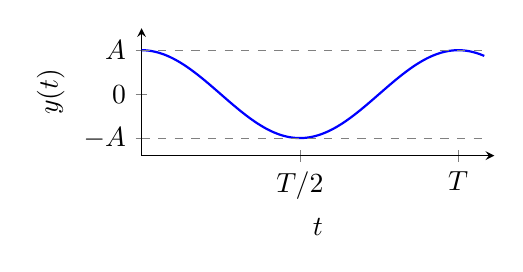
\begin{tikzpicture}
\begin{axis}[
  width=0.5\textwidth, height=3.2cm,
  xlabel={$t$}, ylabel={$y(t)$},
  xmin=0, xmax=7, ymin=-1.4, ymax=1.5,
  xtick={3.1416, 6.2832},
  xticklabels={$T/2$, $T$},
  ytick={-1,0,1}, yticklabels={$-A$,$0$,$A$},
  axis lines=left, samples=200,
]
  \addplot[thick,blue,domain=0:6.8]{cos(deg(x))};
  \draw[dashed,gray] (axis cs:0,1)--(axis cs:6.8,1);
  \draw[dashed,gray] (axis cs:0,-1)--(axis cs:6.8,-1);
\end{axis}
\end{tikzpicture}
\end{center}
\caption{Sinusoidal oscillation with amplitude $A$ and period $T = 2\pi/\omega$.}
\label{fig:shm_cos_ch5}
\end{figure}

\begin{example}[Pendulum with Spring]
A pendulum of length $L$ and mass $m$, with a horizontal spring of spring constant $k$ attached at the pivot end. Find the period of oscillation.

\textbf{Assumptions}: $F_{\text{spring}} = 0$ when $\theta = 0$; small-amplitude oscillations so spring stays horizontal.

Equations of motion in polar coordinates ($r = L = \text{const}$, $\dot{r} = 0$, $\ddot{r} = 0$):

$\hat{r}$-direction:
\[
    mg\cos\theta - T - kx\sin\theta = ma_r = m(\ddot{r} - r\dot{\theta}^2)
\]

$\hat{\theta}$-direction:
\[
    -mg\sin\theta - kx\cos\theta = ma_\theta = m(2\dot{r}\dot{\theta} + r\ddot{\theta})
\]

Small angle: $\sin\theta \approx \theta$, $\cos\theta \approx 1$, $x \approx L\theta$:
\[
    -mg\theta - kL\theta = mL\ddot{\theta}
    \implies -(mg + kL)\theta = mL\ddot{\theta}
\]
\[
    -\left(\frac{g}{L} + \frac{k}{m}\right)\theta = \ddot{\theta}
\]
\[
    \omega = \sqrt{\frac{g}{L} + \frac{k}{m}}
\]
\begin{formula}[Pendulum + Spring Period]
\[
    T = \frac{2\pi}{\sqrt{\dfrac{g}{L} + \dfrac{k}{m}}}
\]
\end{formula}

Check: as $k \to 0$, $\omega \to \sqrt{g/L}$. \checkmark
\end{example}

%───────────────────────────────────────────────────────────────
\section{Conservation of Momentum}
%───────────────────────────────────────────────────────────────

\begin{theorem}[Conservation of Momentum]
For a system with no external forces, $\dv{\vect{P}}{t} = \vect{0}$, so $\vect{P}$ is conserved.
\end{theorem}

Application: measuring the speed of a bullet with little equipment (ballistic pendulum).

\begin{example}[Ballistic Pendulum / Bullet into Block]
A bullet of mass $m$ moving at $v_0$ embeds in a block of mass $M$ on a spring.

Before collision: $\vect{P}_i = mv_0$.

After collision: $\vect{P}_f = (m+M)\vect{v}_i$ (bullet+block move together, spring releases).

By conservation of momentum:
\[
    v_i = \frac{m}{m+M}v_0
\]

The block+bullet then oscillate on the spring:
\[
    -kx = (m+M)\ddot{x}, \quad \omega = \sqrt{\frac{k}{m+M}}
\]
\[
    x(t) = A\cos(\omega t + \phi)
\]
Initial conditions: $x = 0$, $\dot{x} = v_i$ at $t=0$:
\[
    A\cos\phi = 0 \implies \phi = \pi/2
\]
\[
    \dot{x}(0) = v_i = A\omega\cos(0) \implies A = \frac{v_i}{\omega}
\]
\[
    x(t) = \frac{v_i}{\omega}\sin(\omega t)
\]
Maximum distance occurs at $\sin(\omega t) = 1$, i.e.\ $\omega t = \pi/2$:
\[
    x_{\max} = \sqrt{\frac{m+M}{k}}\cdot\frac{m}{m+M}v_0
\]
\[
    v_0 = \frac{\sqrt{k(m+M)}}{m}\,x_{\max}
\]
\end{example}

\begin{example}[Bouncing Ball (Impulse)]
A ball of mass $m$ bouncing off a floor at speed $v$:
\[
    \vect{P}_{\text{before}} = -mv\,\hat{y}, \qquad \vect{P}_{\text{after}} = mv\,\hat{y}
\]
\[
    \Delta\vect{p} = 2mv\,\hat{y}
\]
There is a (large) normal force from the floor. We introduce \emph{impulse}.

Numerical example: $m = 0.2\ \text{kg}$, $v = 8\ \text{m/s}$, contact time $\Delta t = 10^{-3}\ \text{s}$:
\[
    \bar{F} = \frac{2mv}{\Delta t} = \frac{2(0.2)(8)}{10^{-3}} = 3200\ \text{N}
\]
\end{example}

%───────────────────────────────────────────────────────────────
\chapter{Impulse}
%───────────────────────────────────────────────────────────────

\textit{(Saturday, October 21, 2023)}

\section{Impulse}

Given $\vect{F} = \dv{\vect{p}}{t} = m\dv{\vect{v}}{t}$:
\[
    \int_0^t \vect{F}\,dt = \vect{P}(t) - \vect{P}(0)
\]

\begin{definition}[Impulse]
    \[
        \vect{J} = \int_{t_1}^{t_2}\vect{F}\,dt = \int_{t_1}^{t_2}\dv{\vect{p}}{t}\,dt = \vect{p}(t_2) - \vect{p}(t_1) = \Delta\vect{p}
    \]
\end{definition}

When the exact force is not known, it is useful to find the \textbf{average force}:
\[
    F_{\text{av}}\,\Delta t = \int_{t_0}^{t_0+\Delta t}\vect{F}\,dt = \vect{P}(t_0+\Delta t) - \vect{P}(t_0)
\]

\begin{fact}[Gravity and Impulse]
Gravity does create a net impulse, but it is often negligible for short times with high collision forces. Sometimes reframing the situation to remove internal considerations helps.
\end{fact}

\begin{example}[Avoiding Broken Ankles (Landing Force)]
A person falls from height $h$ and decelerates over a distance $s$ (bending knees).

Using kinematics: $v_0 = \sqrt{2gh}$ (speed just before landing). Deceleration phase: $s = \frac{1}{2}a(\Delta t)^2$, $v_0 = a\Delta t$, so $\Delta t = \frac{2s}{v_0}$.

Force during landing:
\[
    F = \frac{Mv_0}{\Delta t} = \frac{Mv_0^2}{2s} \implies F = Mg\frac{h}{s}
\]
Force is linearly proportional to height and inversely to stopping distance --- not an obvious result!
\end{example}

\section{Momentum and Flow of Mass}

Things get tricky when masses combine or explode. Use:
\[
    \int_{t_a}^{t_b}\vect{F}\,dt = \vect{P}(t_b) - \vect{P}(t_a)
\]

\begin{example}[Freight Car and Hopper (Mass Accretion)]
Consider a small time interval $\Delta t$. A hopper drops mass $\Delta m$ (at rest) onto a freight car of mass $M$ moving at velocity $v$.

\[
    P_i = 0 + Mv, \qquad P_f = (M + \Delta m)v
\]
\[
    \Delta P = P_f - P_i = (M + \Delta m)v - Mv = \Delta m\,v
\]
\[
    \frac{\Delta P}{\Delta t} = \frac{\Delta m}{\Delta t}v \implies \dv{P}{t} = \frac{dm}{dt}v = F
\]
For the leaking sand case (mass leaving): $F = 0$ (no external horizontal force).
\end{example}

\begin{fact}[Common Error in Variable-Mass Problems]
Do NOT write:
\[
    F = \dv{p}{t} = \dv{}{t}(mv) = m\dv{v}{t} + v\cdot\dv{m}{t}
\]
This is \textbf{wrong} when $dm/dt \neq 0$, because the second term $v\,\dv{m}{t}$ double-counts momentum. Use impulse--momentum applied to a well-defined system boundary instead.
\end{fact}

%───────────────────────────────────────────────────────────────
\section{Rocket Motion}
%───────────────────────────────────────────────────────────────

A rocket expels mass $\Delta m$ during a time interval $\Delta t$ at exhaust velocity $\vect{u}$ relative to the rocket.

\begin{figure}[H]
\begin{center}
\begin{tikzpicture}[scale=0.95, >=Stealth]
  % === Before (top) ===
  \node[left] at (-0.2,2.5) {\small\textbf{time $t$:}};
  % Rocket body
  \fill[gray!30] (0.5,2.1) rectangle (2.5,2.9);
  \draw[thick] (0.5,2.1) -- (2.5,2.1) -- (2.5,2.9) -- (0.5,2.9) -- cycle;
  \draw[thick] (2.5,2.5) -- (3.0,2.5);  % nozzle
  % Nose cone
  \fill[gray!50] (0.0,2.5) -- (0.5,2.1) -- (0.5,2.9) -- cycle;
  \node at (1.5,2.5) {$M$};
  % Velocity arrow
  \draw[->,thick,blue] (3.0,2.5) -- (4.2,2.5) node[right]{$v$};

  % === After (bottom) ===
  \node[left] at (-0.2,0.8) {\small\textbf{time $t+\Delta t$:}};
  % Rocket body (lighter)
  \fill[gray!30] (0.5,0.4) rectangle (2.2,1.2);
  \draw[thick] (0.5,0.4) -- (2.2,0.4) -- (2.2,1.2) -- (0.5,1.2) -- cycle;
  \draw[thick] (2.2,0.8) -- (2.6,0.8);
  \fill[gray!50] (0.0,0.8) -- (0.5,0.4) -- (0.5,1.2) -- cycle;
  \node at (1.35,0.8) {$M{-}\Delta m$};
  % Rocket velocity
  \draw[->,thick,blue] (2.6,0.8) -- (3.9,0.8) node[right]{$v{+}\Delta v$};
  % Exhaust gas
  \fill[orange!40] (2.8,0.55) rectangle (3.8,0.35);
  \draw[thick,orange] (2.8,0.55) rectangle (3.8,0.35);
  \node[below,orange,scale=0.8] at (3.3,0.35) {$\Delta m$};
  \draw[->,thick,orange] (2.8,0.45) -- (1.8,0.45) node[left,scale=0.8]{exhaust $u$};
\end{tikzpicture}
\end{center}
\caption{Rocket of mass $M$ moving at $v$ (top). After $\Delta t$ (bottom): rocket has mass $M-\Delta m$ at speed $v+\Delta v$, expelled gas $\Delta m$ moves backward at exhaust speed $u$ relative to rocket.}
\label{fig:rocket}
\end{figure}

\[
    p(t) = (M + \Delta m)v
\]
\[
    p(t+\Delta t) = (v+\Delta v)M + \Delta m(v + \Delta v + u)
\]
\[
    p(t+\Delta t) - p(t) = MV + M\Delta v + \Delta m\,v + \Delta m\,\Delta v + \Delta m\,u - Mv - \Delta m\,v
    = M\Delta v + \Delta m(\Delta v + u)
\]

As $\Delta t \to 0$, the non-first-order term $\Delta m\,\Delta v$ vanishes (\textbf{Physics Tip: non-first-order terms vanish in the limit}):
\[
    \dv{p}{t} = M\dv{v}{t} + \frac{dm}{dt}\cdot u
\]

By conservation of momentum (no external force): with mass conservation $\dv{M}{t} = -\dv{m_{\text{exhaust}}}{t}$:

\begin{formula}[Rocket Equation]
\[
    M\dv{v}{t} = -u\dv{M}{dt} = u\dv{m_{\text{exhaust}}}{dt}
\]
\end{formula}

\subsection{Integrating the Rocket Equation}

\[
    \dv{v}{t} = \frac{u}{M}\dv{M}{dt}
\]
\[
    \int_{t_0}^{t_f}\dv{v}{t}\,dt = u\int_{M_0}^{M_f}\frac{1}{M}\,dM
\]
\[
    v_f - v_0 = u\ln\frac{M_f}{M_0} = -u\ln\!\left(\frac{M_0}{M_f}\right)
\]

\begin{formula}[Tsiolkovsky Rocket Equation (No Gravity)]
If $v_0 = 0$:
\[
    v_f = -u\ln\!\left(\frac{M_0}{M_f}\right) = u\ln\!\left(\frac{M_0}{M_f}\right)
\]
(taking $u$ as the magnitude of exhaust speed, with exhaust directed backward).
\end{formula}

\textbf{Including gravity}:
\[
    Mg = M\dv{v}{t} - u\dv{M}{dt} \quad (\text{thrust} = u\dv{M}{dt})
\]
\[
    \dv{v}{t} = \frac{u}{M}\dv{M}{dt} + g
\]
Integrating:
\[
    \int_{v_0}^{v_f}dv = u\int_{M_0}^{M_f}\frac{1}{M}\,dM + g\Delta t
\]
\begin{formula}[Rocket Equation with Gravity]
\[
    v_f = -u\ln\!\left(\frac{M_f}{M_0}\right) + g t_f \quad (v_0 = 0)
\]
\end{formula}

%───────────────────────────────────────────────────────────────
\chapter{Momentum Flow, Force, and Work-Energy Theorem}
%───────────────────────────────────────────────────────────────

\section{Momentum Flow and Force}

\textit{(Thursday, October 26, 2023)}

Consider the impulse of catching a small droplet of water ($v_f = 0$):
\[
    I_{\text{droplet}} = \int_{\text{collision}} F\,dt = \Delta p = m(v_f - v) = -mv
\]
So impulse on droplet $= -mv$. By Newton's 3rd law:
\[
    I_{\text{nozzle}} = mv
\]
If there are multiple collisions per second (period $T$ between collisions):
\[
    F_{\text{av}}\cdot T = \int_{\text{collision}} F\,dt = mv
\]
\begin{formula}[Average Force from Droplet Stream]
\[
    F_{\text{av}} = \frac{mv}{T} = \frac{mv^2}{\ell}, \quad \ell = vT
\]
(Note: this is the same form as the centripetal force $mv^2/r$ in circular motion!)
\end{formula}

\section{Momentum Flux}

\begin{definition}[Momentum Flux]
The average momentum per unit length is $mv/\ell$. The momentum flux (rate of momentum transport) is:
\[
    \frac{mv}{\ell}\cdot v = \frac{mv^2}{\ell} = \frac{mv}{T}
\]
For a continuous stream of matter with cross-sectional area $A$, speed $v$, in direction $\hat{v}$, and mass density $\rho_m$:
\[
    \dot{\vect{p}} = \rho_m v^2 A\,\hat{v}
\]
where $\dot{\vect{p}}$ is the rate at which momentum flows through a hypothetical surface across the stream.
\end{definition}

\begin{figure}[H]
\begin{center}
\begin{tikzpicture}[scale=0.9, >=Stealth]
  % Surface (vertical wall)
  \fill[pattern=north east lines] (3.5,-0.5) rectangle (3.8,1.5);
  \draw[thick] (3.5,-0.5) -- (3.5,1.5);
  % Stream arrows (flow to right)
  \foreach \y in {0.1, 0.5, 0.9} {
    \draw[->,thick,blue] (0.3,\y) -- (2.5,\y);
    \fill[blue!30] (0.5,\y-0.12) rectangle (1.8,\y+0.12);
  }
  \node[above] at (1.3,1.1) {$\rho,\, v$};
  % Cross section label
  \draw[<->] (0.3,-0.3) -- (0.3,1.1) node[midway,left]{$A$};
  % Force on wall
  \draw[->,thick,red] (3.5,0.5) -- (4.5,0.5) node[right]{$\dot{p} = \rho v^2 A$};
\end{tikzpicture}
\end{center}
\caption{A stream of matter (density $\rho$, speed $v$, cross-section $A$) impinges on a surface. The momentum flux $\dot{p} = \rho v^2 A$ is the force exerted on the surface.}
\label{fig:momentum_flux}
\end{figure}

By Newton's 3rd law, the force on the surface on the stream is:
\[
    \vect{P}_{\text{surface on stream}} = -\rho_m v^2 A\,\hat{v}
\]

\begin{example}[Lennard-Jones Force (Momentum Flux Context)]
The Lennard-Jones potential between two particles separated by $r$:
\[
    V(r) = 4\varepsilon\left[\left(\frac{\sigma}{r}\right)^{12} - \left(\frac{\sigma}{r}\right)^6\right]
\]
The corresponding force:
\begin{align*}
    F(r) &= -\dv{V}{r} = 4\varepsilon\left(\frac{-12\sigma^{12}}{r^{13}} + \frac{6\sigma^6}{r^7}\right) \\
    &= 48\varepsilon\left(\frac{\sigma^{12}}{r^{13}} - \frac{\sigma^6}{2r^7}\right)
\end{align*}
Let $\beta = \sigma^6/r^6$:
\[
    = \frac{48\varepsilon}{r}\beta\left(\beta - \frac{1}{2}\right)
\]
\begin{formula}[Lennard-Jones Force]
\[
    F(r) = \frac{48\varepsilon}{r}\,\beta\!\left(\beta - \frac{1}{2}\right), \quad \beta = \frac{\sigma^6}{r^6}
\]
\end{formula}
\end{example}

%───────────────────────────────────────────────────────────────
\chapter{Work and Energy}
%───────────────────────────────────────────────────────────────

\textit{(Energy 2, Tuesday October 24, 2023)}

\section{Work-Energy Theorem (Review)}

\begin{formula}[Work-Energy Theorem]
\[
    W = \int_{x_i}^{x_f} F\,dx = \frac{1}{2}mv_f^2 - \frac{1}{2}mv_i^2
\]
\end{formula}

\begin{example}[Ball Under Gravity — Two Methods]
A ball thrown upward at speed $v_0$. Maximum height $h$:

\textbf{Kinematics}: $t_f = v_0/g$, $h = -\frac{1}{2}g(v_0/g)^2 + v_0(v_0/g) = \frac{v_0^2}{2g}$.

\textbf{Work-energy}:
\[
    \int_0^h F\,dx = \int_0^h (-mg)\,dx = -mgh = \frac{1}{2}m(v_f^2 - v_i^2) = -\frac{1}{2}mv_0^2
\]
\[
    \implies h = \frac{v_0^2}{2g} \quad \checkmark
\]
\end{example}

\begin{example}[Falling Weight Demo]
A mass falls from height $h$. Work-energy gives:
\[
    \int_h^0 (-mg)\,dx = \frac{1}{2}m(v_f^2 - v_0^2)
\]
\[
    mgh = \frac{1}{2}mv_f^2 \implies v_f = \sqrt{2gh}
\]
For the pendulum: the tension does no work since $\vect{T}\perp\dot{\vect{x}}$.
\end{example}

\begin{example}[Escape Velocity]
What velocity is needed for a projectile to escape Earth's gravitational field? (Escape from radius $r_e$, $v_f \to 0$ at $r \to \infty$.)
\[
    \int F\,dx = -GmM\int_{r_e}^{\infty}\frac{dr}{r^2} = \frac{1}{2}mv_f^2 - \frac{1}{2}mv_i^2
\]
\[
    -\frac{GmM}{r_e} = -\frac{1}{2}mv_i^2 \quad (\text{to escape, }\tfrac{1}{2}mv_f^2 > 0)
\]
\[
    \frac{1}{2}mv_i^2 - \frac{GmM}{r_e} > 0 \implies v_i^2 > \frac{2GM}{r_e}
\]
\begin{formula}[Escape Velocity]
\[
    v_i > \sqrt{\frac{2GM}{r_e}}
\]
\end{formula}
\end{example}

\begin{example}[Spring and SHO via Work-Energy]
$\Delta x = A\cos(\omega t + \phi)$, $\phi = \pi/2$ (from $x=0$ initial condition):
\[
    \int_0^{x_f} F\,dx = -\int_0^{x_f} kx\,dx = -\frac{1}{2}kx_f^2
\]
\[
    -\frac{1}{2}kx_f^2 = \frac{1}{2}mv_f^2 - \frac{1}{2}mv_i^2 \implies kx_f^2 = mv_i^2
\]
\[
    x_f = \sqrt{\frac{m}{k}}\,v_i \quad \checkmark
\]
\end{example}

\section{Definitions: Energy}

\begin{definition}[Kinetic Energy]
    \[
        KE = \frac{1}{2}mv^2 \quad \text{(valid only at non-relativistic speeds)}
    \]
\end{definition}

\begin{definition}[Potential Energy]
\begin{itemize}
    \item Constant gravity: $U = mgh$
    \item Varying gravity: $U = -\displaystyle\int_{r_i}^{r_f}\frac{GmM}{r^2}\,dr$
    \item Spring: $U = \frac{1}{2}k\Delta x^2$
\end{itemize}
\end{definition}

\begin{formula}[Work-Energy Theorem (General)]
\[
    W = \int \vect{F}\cdot d\vect{r} = \frac{1}{2}mv_f^2 - \frac{1}{2}mv_i^2 = \Delta KE
\]
\end{formula}

\textbf{Extension to 3D}:
\[
    W = \int_C \vect{F}\cdot d\vect{r} \quad (C: \text{ curve of path})
\]

\begin{definition}[Power]
    \[
        P = \dv{W}{t} = \vect{F}\cdot\vect{v}
    \]
    Example (power due to gravity on an object moving at angle $\theta$ from horizontal at speed $v_0$):
    \[
        P = mgv_0\cos(\theta + 90°) = -mgv_0\sin\theta
    \]
\end{definition}

\section{Limitations of the Work-Energy Theorem}

\begin{fact}[Work-Energy Theorem Requires Conservative Forces]
The work-energy theorem only works for \textbf{conservative forces}. For a closed path:
\[
    W = \oint \vect{F}\cdot d\vect{r} = 0 \implies \frac{1}{2}mv_f^2 = \frac{1}{2}mv_i^2
\]
This makes sense for gravity (if a ball starts and ends at height $h$, net work by gravity is zero).

\textbf{Friction} is non-conservative: work depends on path length, so it does not conserve mechanical energy. More research needed into friction at the microscopic level.
\end{fact}

% Unit 3.5-4: Momentum Flow (continued), Energy, Work & Energy, Conservative Forces
% Pages 66–92

\chapter{Momentum Flow and Pressure}

\section{Momentum Flux Density}

If the surface is \emph{not} perpendicular to the flow, the momentum rate is
\[
    \dot{P} = \rho_m v^2 A \cos\theta.
\]

\begin{definition}[Flux Density of the Stream]
The momentum flux density $\vect{J}$ of a stream is
\[
    \vect{J} = \rho_m v^2 \,\uvect{v}.
\]
\end{definition}

If one lets $\vect{A}$ be a vector perpendicular to the surface with magnitude equal to the area, then
\[
    \dot{\vect{P}} = (\vect{J} \cdot \vect{A})\,\uvect{v}.
\]

\begin{itemize}
    \item Flux is \textbf{positive} when $\vect{J} \cdot \vect{A} > 0$; flux is \textbf{negative} when $\vect{J} \cdot \vect{A} < 0$.
    \item The total force on a system due to a number of sources of momentum flow is
    \[
        F_{\text{tot}} = \sum_k \dot{P}_k = \sum_k (\vect{J} \cdot \vect{A}_k)\,\uvect{v}_k.
    \]
    \item As the number of elements increases, this sum becomes a \textbf{surface integral}.
\end{itemize}

A more helpful way to calculate the force on a system with several sources of momentum flow is
\begin{formula}[Total Force from Momentum Flow]
\[
    F_{\text{tot}} = \dot{P}_{\text{in}} - \dot{P}_{\text{out}}.
\]
\end{formula}

\begin{example}[Pressure of a Gas]
Consider a box of $n$ particles each with mass $m$.

\begin{figure}[H]
    \centering
    \caption{Box of gas particles; surface $A$ on one face.}
\end{figure}

We want to find the momentum transport through a surface $A$.

At any moment the density of particles moving \emph{toward} the wall is $\rho/2$, so
\[
    \dot{P}_x = \frac{\rho}{2}\,v_x^2\,A.
\]
The $v_x$ here is the $x$-component of velocity.

Momentum flow \emph{away} from the wall:
\[
    \dot{P}_{-x} = \frac{\rho}{2}\,v_x^2\,A.
\]
Thus
\[
    F_x = \dot{P}_x - \dot{P}_{-x} = \rho v^2 A.
\]

For arbitrary velocities (using averages):
\[
    \widetilde{F}_x = \dot{P}_x - \dot{P}_{-x} = \rho\,\overline{v_x^2}\,A.
\]

The pressure is
\[
    \mathcal{P} = \frac{F}{A} = \rho\,\overline{v_x^2}.
\]

Since $\overline{v^2} = \overline{v_x^2} + \overline{v_y^2} + \overline{v_z^2}$ and by isotropy each component is equal,
\begin{formula}[Gas Pressure]
\[
    \boxed{\mathcal{P} = \frac{1}{3}\,\rho\,\overline{v^2}.}
\]
\end{formula}
\end{example}

\begin{example}[Pressure on a Dike]
A curved dike deflects a stream of fluid through an angle $\Delta\theta$. Let the incoming momentum flux be
\[
    \dot{P}_{\text{in}} = \rho v^2 A \,\uvect{v}_c, \qquad \dot{P}_{\text{out}} = \rho v^2 A\,\uvect{v}_d.
\]
So
\[
    \dot{P} = \rho v^2 A\,(\uvect{v}_c - \uvect{v}_d) = \rho v^2 A \bigl(2\sin(\Delta\theta/2)\bigr).
\]
The force per unit area (pressure) on the dike element of length $R\,\Delta\theta$ and height $h$ is
\[
    \mathcal{P} \approx \frac{\dot{P}}{R\,\Delta\theta \cdot h} = \frac{\rho v^2 A\,\Delta\theta}{R\,\Delta\theta\, h} = \frac{\rho v^2 A}{R\,h} = \frac{\rho v^2 w}{R},
\]
where $w = A/h$ is the width.
\end{example}

\chapter{Energy}

\section{Work–Energy Theorem in One Dimension}

Force is often known as a function of \emph{position}, not time. Many problems take the form
\[
    m\,\dv{v}{t} = F(x).
\]
To solve, integrate both sides with respect to $x$:
\[
    m \int_{x_a}^{x_b} \dv{v}{t}\,dx = \int_{x_a}^{x_b} F(x)\,dx.
\]
Replace $dx$:
\[
    dx = \left(\dv{x}{t}\right)dt = v\,dt,
\]
so
\begin{align*}
    m\int_{x_a}^{x_b}\dv{v}{t}\,dx &= m\int_{t_a}^{t_b} \dv{v}{t}\,v\,dt \\
    &= m\int_{t_a}^{t_b} \dv{}{t}\!\left(\tfrac{1}{2}v^2\right)dt \\
    &= \tfrac{1}{2}mv^2\Big|_{t_a}^{t_b}.
\end{align*}

\begin{formula}[Work–Energy Theorem (1D)]
\[
    \boxed{\tfrac{1}{2}mv_b^2 - \tfrac{1}{2}mv_a^2 = \int_{x_a}^{x_b} F(x)\,dx.}
\]
\end{formula}

\subsection{Derivation of GPE near Earth's Surface}

\[
    \tfrac{1}{2}mv_b^2 - \tfrac{1}{2}mv_a^2 = -mg\int_{x_a}^{x_b} dx = -mg(x_b - x_a).
\]
Letting $v_a = v_b = 0$ gives $\tfrac{1}{2}mv_a^2 = mgh$.

\subsection{Derivation of Spring Potential Energy}

\begin{figure}[H]
\begin{center}
\begin{tikzpicture}[scale=0.9, >=Stealth]
  % Wall
  \fill[pattern=north east lines] (-0.2,-0.35) rectangle (0,0.35);
  \draw[thick] (0,-0.35) -- (0,0.35);
  % Spring
  \draw[thick, decorate, decoration={zigzag, segment length=5pt, amplitude=3pt}]
    (0,0) -- (2.8,0);
  % Mass
  \fill[gray!40] (2.8,-0.3) rectangle (3.4,0.3);
  \draw[thick] (2.8,-0.3) rectangle (3.4,0.3);
  \node at (3.1,0) {$M$};
  % Displacement arrow
  \draw[<->,blue] (0,-0.6) -- (3.1,-0.6) node[midway,below]{$x_0$};
  % Equilibrium dashed line
  \draw[dashed,gray] (1.8,-0.5) -- (1.8,0.5) node[above,scale=0.8]{equil.};
\end{tikzpicture}
\end{center}
\caption{Mass on a spring; equilibrium at $x=0$, initial displacement $x_0$ from equilibrium.}
\label{fig:spring_pe}
\end{figure}

With $F = -kx$:
\[
    \tfrac{1}{2}Mv^2 - \tfrac{1}{2}Mv_0^2 = -k\int_{x_0}^{x} x\,dx = -\tfrac{1}{2}kx^2 + \tfrac{1}{2}kx_0^2,
\]
thus
\[
    v^2 = \frac{k}{M}(x_0^2 - x^2).
\]
Separating variables:
\[
    \frac{1}{\sqrt{x_0^2 - x^2}}\,dx = \sqrt{\frac{k}{M}}\,dt,
\]
\[
    \sin^{-1}\!\left(\frac{x}{x_0}\right) - \sin^{-1}(1) = \omega t,
\]
\begin{formula}[SHO Solution from Energy]
\[
    \boxed{x = x_0 \sin\!\left(\omega t + \tfrac{\pi}{2}\right) = x_0\cos(\omega t).}
\]
\end{formula}

\section{Work and Energy}

\begin{definition}[Kinetic Energy]
\[
    K_a \defeq \tfrac{1}{2}Mv_a^2.
\]
\end{definition}

\begin{definition}[Work]
\[
    W_{ba} \defeq \int_{x_a}^{x_b} F\,dx = K_b - K_a \quad \text{(Work–Energy Theorem)}.
\]
\end{definition}

Units of energy: Joule, $\mathrm{J} = \frac{\mathrm{kg}\cdot\mathrm{m}^2}{\mathrm{s}^2} = \frac{M \cdot L^2}{T^2}$.

\section{Integrating Motion in Several Directions}

Let $\vect{r}$ be a position vector. We need to solve
\[
    \vect{F}(\vect{r}) = m\dv{\vect{v}}{t}.
\]
Dot both sides with $\Delta\vect{r}$:
\[
    \vect{F} \cdot \Delta\vect{r} = m\dv{\vect{v}}{t} \cdot \Delta\vect{r} = F\,\Delta r\cos\theta = m\dv{\vect{v}}{t}\cdot\Delta\vect{r}.
\]

Since $\Delta\vect{r} = \vect{v}\,\Delta t$ (reason why energy is path-independent!):
\[
    m\dv{\vect{v}}{t}\cdot\Delta\vect{r} = m\dv{\vect{v}}{t}\cdot\vect{v}\,\Delta t = m\,\frac{1}{2}\dv{}{t}(v^2)\,\Delta t.
\]
Thus
\[
    \vect{F}\cdot\Delta\vect{r} = \frac{m}{2}\dv{}{t}(v^2)\,\Delta t.
\]

Next, divide the trajectory from $\vect{r}_a$ to $\vect{r}_b$ into short segments:

\begin{figure}[H]
    \centering
    \caption{Trajectory divided into short segments $\Delta\vect{r}_j$ at positions $\vect{r}_j$.}
\end{figure}

Thus $\vect{F}(\vect{r}_j)\cdot\Delta\vect{r}_j = \dfrac{m}{2}\dv{}{t}(v_j^2)\,\Delta t_j$.

Summing:
\[
    \sum_{j=1}^{N} \vect{F}(\vect{r}_j)\cdot\Delta\vect{r}_j = \sum_{j=1}^{N} \frac{m}{2}\dv{}{t}(v_j^2)\,\Delta t_j.
\]
In the limit:
\[
    \int_{\vect{r}_a}^{\vect{r}_b} \vect{F}(\vect{r})\cdot d\vect{r} = \frac{m}{2}\int_{t_a}^{t_b}\dv{}{t}(v^2)\,dt = \frac{m}{2}\,v^2\Big|_{t_a}^{t_b} = \tfrac{1}{2}mv_b^2 - \tfrac{1}{2}mv_a^2.
\]

\begin{formula}[Work–Energy Theorem (3D)]
\[
    \boxed{\int_{\vect{r}_a}^{\vect{r}_b} \vect{F}\cdot d\vect{r} = \tfrac{1}{2}mv_b^2 - \tfrac{1}{2}mv_a^2.}
\]
\end{formula}

\begin{example}[General Escape Velocity]
The gravitational force on a mass $m$ due to a planet of mass $M_e$ is
\[
    \vect{F} = -\frac{GM_e m}{r^2}\,\uvect{r} = -mg\frac{R_e^2}{r^2}\,\uvect{r}.
\]
In spherical coordinates, $d\vect{r} = dr\,\uvect{r} + r\,d\theta\,\tthat$, so
\[
    \vect{F}\cdot d\vect{r} = -mg\frac{R_e^2}{r^2}\,dr \quad (\text{since } \uvect{r}\cdot\tthat = 0).
\]
Thus
\[
    \tfrac{1}{2}mv_f^2 - \tfrac{1}{2}mv_0^2 = -mgR_e^2\int_{R_e}^{r}\frac{dr}{r^2} = -mgR_e^2\left(\frac{1}{r} - \frac{1}{R_e}\right).
\]
As $r\to\infty$:
\begin{formula}[Escape Velocity]
\[
    v_{\text{esc}} = \sqrt{2g R_e}.
\]
\end{formula}
\end{example}

\section{Applying the Work–Energy Theorem}

Because $W_{ba} = \int_a^b \vect{F}\cdot d\vect{r}$ for non-conservative forces, $\vect{F}$ and the actual path must be known.

\begin{itemize}
    \item Most forces are conservative, however.
    \item When motion is \emph{constrained}, the constraint force does no work (the force integral only depends on tangential forces).
\end{itemize}

\begin{definition}[Work (general)]
\[
    \int_C \vect{F}\cdot d\vect{r} = W.
\]
\end{definition}

\begin{definition}[Power]
\[
    \dv{W}{t} = \vect{F}\cdot\vect{v}.
\]
\end{definition}

\section{Conservation of Energy}

\begin{formula}[Conservation of Energy]
\[
    W = \int_{\vect{r}_a}^{\vect{r}_b} \vect{F}\cdot d\vect{r} = -U(\vect{r}_b) + U(\vect{r}_a) = K_b - K_a,
\]
\[
    \Rightarrow\quad K_a + U(\vect{r}_a) = K_b + U(\vect{r}_b) \quad \text{(total energy is conserved)}.
\]
\end{formula}

For a closed path, $W = \oint_C \vect{F}\cdot d\vect{r} = U(\vect{r}_a) - U(\vect{r}_a) = 0$.

Thus:
\[
    U = -\oint \vect{F}\cdot d\vect{r}, \qquad \vect{F} = -\grad U, \qquad F = -\dv{U}{r}.
\]

\section{Energy Diagrams}

\begin{figure}[H]
\begin{center}
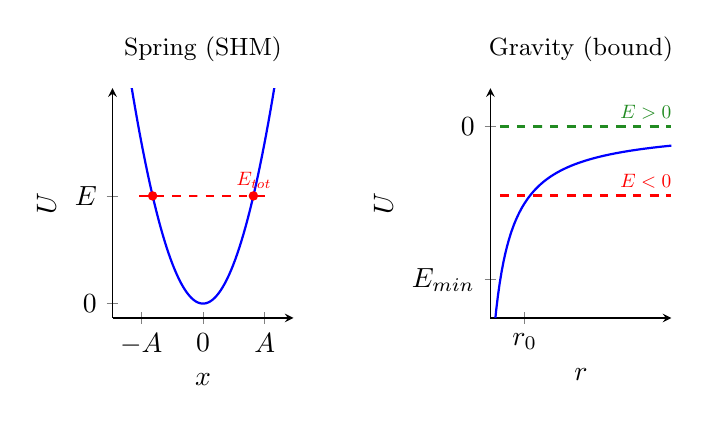
\begin{tikzpicture}
  %--- Left: SHM parabola ---
  \begin{scope}
  \begin{axis}[
    name=ax1,
    width=0.32\textwidth, height=4.5cm,
    xlabel={$x$}, ylabel={$U$},
    title={\small Spring (SHM)},
    xmin=-2.2,xmax=2.2, ymin=-0.2, ymax=3,
    xtick={-1.5,0,1.5}, xticklabels={$-A$,$0$,$A$},
    ytick={0,1.5}, yticklabels={$0$,$E$},
    axis lines=left, samples=80,
  ]
    \addplot[thick,blue,domain=-2:2]{x^2};
    \addplot[thick,dashed,red,domain=-1.55:1.55]{1.5} node[pos=0.9,above,scale=0.7]{$E_\text{tot}$};
    \addplot[only marks,mark=*,mark size=1.5pt,red] coordinates {(-1.225,1.5)(1.225,1.5)};
  \end{axis}
  \end{scope}
  %--- Center: gravitational potential well ---
  \begin{scope}[xshift=4.8cm]
  \begin{axis}[
    name=ax2,
    width=0.32\textwidth, height=4.5cm,
    xlabel={$r$}, ylabel={$U$},
    title={\small Gravity (bound)},
    xmin=0.3, xmax=4, ymin=-2.5, ymax=0.5,
    xtick={1}, xticklabels={$r_0$},
    ytick={-2,0}, yticklabels={$E_\text{min}$,$0$},
    axis lines=left, samples=100,
  ]
    \addplot[thick,blue,domain=0.38:4]{-1/x};
    \addplot[thick,dashed,red,domain=0.5:4]{-0.9} node[pos=0.85,above,scale=0.7]{$E<0$};
    \addplot[thick,dashed,ForestGreen,domain=0.5:4]{0.0} node[pos=0.85,above,scale=0.7]{$E>0$};
  \end{axis}
  \end{scope}
\end{tikzpicture}
\end{center}
\caption{Energy diagrams. \textit{Left}: Spring force — parabolic $U(x) = kx^2/2$; $E_{\text{tot}}$ is a horizontal red dashed line and the amplitude (turning points) is where $KE=0$. \textit{Right}: Gravitational $U(r) = -GMm/r$; bound orbit has $E<0$ (red dashed), unbound orbit has $E>0$ (green dashed).}
\label{fig:energy_diagrams}
\end{figure}

Non-conservative forces: $\oint \vect{F}\cdot d\vect{r} \neq 0$ (depends on path taken). Example: friction.

Thus,
\[
    E_{\text{tot}} = U + K + W_{\text{non-cons.}} = U + K + \int_{\vect{a}}^{\vect{b}} \vect{F}_f \cdot d\vect{r}.
\]

\begin{example}[Block on an Incline]
\begin{figure}[H]
    \centering
    \caption{Block sliding down an incline of angle $\theta$ and height $h$, path length $s = h/\sin\theta$.}
\end{figure}

\begin{itemize}
    \item Start: $U_a = mgh$, $K_a = 0$, $E_a = U_a + K_a = mgh$.
    \item End: $U_b = 0$, $K_b = \tfrac{1}{2}mv_b^2$, $E_b = \tfrac{1}{2}v_b^2$.
    \item Work by friction:
    \[
        W_f = \int_a^b \vect{F}_{fr}\cdot d\vect{r} = -\int_a^b \mu F_N\,ds = -\mu mg\cos\theta \cdot s = -\mu mg\cos\theta \cdot \frac{h}{\sin\theta}.
    \]
\end{itemize}
\end{example}

\chapter{Additional Energy Examples}

\section{Minimum Height for Ball to Go Around a Loop}

\begin{figure}[H]
\begin{center}
\begin{tikzpicture}[scale=0.85, >=Stealth]
  % Ground level
  \draw[thick] (0,0) -- (7.5,0);
  % Ramp (inclined)
  \draw[thick] (0,3.0) -- (2.2,0);
  % Height label
  \draw[<->,gray] (-0.3,0) -- (-0.3,3.0) node[midway,left]{$h$};
  % Ball on ramp
  \fill[blue!60] (0.9,1.5) circle[radius=0.13];
  % Loop circle
  \draw[thick] (5.0,1.0) circle[radius=1.0];
  % Center of loop
  \fill (5.0,1.0) circle[radius=0.04];
  % Radius label
  \draw[<->,gray] (5.0,1.0) -- (5.0,2.0) node[midway,right]{$R$};
  % Ball at top of loop
  \fill[blue!60] (5.0,2.0) circle[radius=0.13];
  % Force arrow at top
  \draw[->,red] (5.0,2.0) -- (5.0,1.4) node[right,scale=0.8]{$mg+N$};
  % Height 2R label
  \draw[<->,gray] (4.1,0) -- (4.1,2.0) node[midway,left]{$2R$};
  % Ball at bottom
  \fill[blue!60] (4.0,0) circle[radius=0.13];
\end{tikzpicture}
\end{center}
\caption{Ball released from height $h$ slides down a frictionless ramp and around a loop of radius $R$. At the top of the loop (height $2R$) the centripetal condition requires $N + mg = mv_t^2/R$.}
\label{fig:loop_the_loop}
\end{figure}

Total energy: $mgh$.

At the bottom of the loop: $\tfrac{1}{2}mv^2 = mgh \Rightarrow v = \sqrt{2gh}$.

We want the ball to make it all the way around without falling at the top.

At the top of the loop (height $2R$), the centripetal force equation is:
\[
    mg + N = m\frac{v_t^2}{R}.
\]
We want $N \geq 0$, so
\[
    \frac{mv_t^2}{R} \geq mg.
\]
By energy conservation from start to top:
\[
    mg(h - 2R) = \tfrac{1}{2}mv_t^2 \Rightarrow v_t^2 = 2g(h-2R).
\]
Substituting into the constraint:
\[
    \frac{m \cdot 2g(h-2R)}{R} - mg \geq 0,
\]
\[
    \frac{m\,g(h-2R)}{R} \cdot 2 \geq mg,
\]
\[
    2h - 4R \geq R, \qquad 2h \geq 5R,
\]
\begin{formula}[Minimum Height for Loop]
\[
    \boxed{h > \frac{5}{2}R.}
\]
\end{formula}

\subsection{Higgs Potential}

\begin{itemize}
    \item A particle that originally gives other particles mass.
    \item Discovered at CERN LHC.
    \item Smashes particles together to discover their properties.
\end{itemize}

\section{Integrating \texorpdfstring{$\vect{F}\cdot d\vect{r}$}{F dot dr}}

\begin{figure}[H]
    \centering
    \caption{For circular motion, break $d\vect{r}$ into $(A\,\uvect{r} + B\,\tthat)$. Tip: $|d\vect{r}| \approx \ell\,d\theta$ for radius $\ell$.}
\end{figure}

\subsection{Work Done by a Central Force}

\[
    W_{ba} = \int_a^b \vect{F}\cdot d\vect{r} = \int_a^b f(r)\,\uvect{r}\cdot(dr\,\uvect{r} + r\,d\theta\,\tthat) = \int_a^b f(r)\,dr.
\]
This depends \emph{only} on initial and final $r$. Thus, work done by a central force on a closed path is $\mathbf{0}$.

\subsection{Work Done by Friction}

\[
    W_{ba} = -\int_{r_a}^{r_b} f\,ds = -f\,S,
\]
where $S$ is the total length of the path.

\section{Conservation of Mechanical Energy}

\[
    \int_{r_a}^{r_b} \vect{F}\cdot d\vect{r} = -U(\vect{r}_b) + U(\vect{r}_a)
\]
(implies conservative force $\vect{F}$ around a closed path is $0$).

But also $W_{ba} = K_b - K_a$, so:
\[
    K_a + U_a = K_b + U_b \quad \longrightarrow \text{ conservation of mechanical energy}.
\]

\begin{example}[Energy Solution to the Pendulum Problem]
\begin{figure}[H]
    \centering
    \caption{Pendulum of length $\ell$, angle $\theta$ from vertical, height $y = \ell(1-\cos\theta)$.}
\end{figure}

Total energy:
\[
    E = K + U = \tfrac{1}{2}m\ell^2\dot{\theta}^2 + mgy = \tfrac{1}{2}m\ell^2\dot{\theta}^2 + mg\ell(1-\cos\theta).
\]
At $\dot{\theta} = 0$ (end of swing at angle $\theta_0$):
\[
    E_f = mg\ell(1-\cos\theta_0).
\]
By conservation of energy:
\[
    \tfrac{1}{2}m\ell^2\dot{\theta}^2 + mg\ell(1-\cos\theta) = mg\ell(1-\cos\theta_0),
\]
\[
    \dot{\theta} = \dv{\theta}{t} = \sqrt{\frac{2g}{\ell}(\cos\theta - \cos\theta_0)}.
\]
Separating variables:
\[
    \int \frac{d\theta}{\sqrt{\cos\theta - \cos\theta_0}} = \sqrt{\frac{2g}{\ell}}\int dt.
\]
Using the small-angle approximation $\cos\theta \approx 1 - \tfrac{1}{2}\theta^2$:
\[
    \int \frac{d\theta}{\sqrt{\tfrac{1}{2}(\theta_0^2 - \theta^2)}} = \sqrt{\frac{2g}{\ell}}\int dt \qquad \Rightarrow \omega = \sqrt{\frac{g}{\ell}}.
\]
Substituting $u = \theta/\theta_0$:
\[
    \int_0^{\theta}\frac{d\theta}{\theta_0\sqrt{1-(\theta/\theta_0)^2}} = \omega\int_0^t dt,
\]
\[
    \sin^{-1}(\theta/\theta_0) = \sqrt{\frac{g}{\ell}}\,(t - 0).
\]
\begin{formula}[Pendulum Solution]
\[
    \boxed{\theta = \theta_0 \sin(\omega t).}
\]
\end{formula}
\end{example}

\section{Potential Energy}

\subsection{Uniform Gravitational Field}

In a uniform gravitational field, $\vect{F} = -mg\,\khat$:
\[
    U_b - U_a = -\int_{z_a}^{z_b}(-mg)\,dz = mg(z_b - z_a).
\]

\begin{formula}[Potential Energy Difference]
\[
    U_b - U_a = -\int_{r_a}^{r_b} \vect{F}\cdot d\vect{r} = -\int_{r_a}^{r_b} f(r)\,dr.
\]
\end{formula}

The negative sign comes from the definition of potential energy: the work needed to bring the system from $r_i$ to $\infty$.

\begin{example}[Bead, Hoop, and Spring]
A bead of mass $m$ sits on a spring of constant $k$ at the bottom of a hoop of radius $2R$. The spring is compressed by $2R$.

\begin{figure}[H]
    \centering
    \caption{Bead on a hoop with a spring at the bottom; the bead is launched and exits at the top.}
\end{figure}

Initial energy:
\[
    E_i = mg(2R) + \tfrac{1}{2}k(2R)^2 = 2kR^2 + mg(2R).
\]
Final energy (at top, speed $v_f$):
\[
    E_f = \tfrac{1}{2}mv_f^2.
\]
By conservation:
\[
    v_f = 2\sqrt{gR + \frac{kR^2}{m}}.
\]
\end{example}

\subsection{What Potential Tells Us About Force}

From the definition:
\[
    U_b - U_a = \int_a^b F(x)\cdot dx \quad \Rightarrow \quad U_b = \int_a^b F(x)\,dx + U_a.
\]
Thus
\[
    U(x) = -\int_a^x F(x')\,dx' + U_a = -\int F(x)\,dx.
\]
Examining $U(x + \Delta x) - U(x)$:
\[
    \approx -\int [F(x+\Delta x) - F(x)]\,dx \approx -F(x)\,(x + \Delta x - x) = -F(x)\,\Delta x.
\]

\begin{formula}[Force from Potential]
\[
    \boxed{F(x) = -\dv{U}{x}.}
\]
\end{formula}

\section{Energy Diagrams (Detailed)}

\begin{figure}[H]
    \centering
    \caption{Energy diagram showing $U(r)$, $KE$, and $E_{\text{tot}}$. Bounded motion: $r$ can get arbitrarily large but is bounded by $r_{\max}$. Unbounded: there exists an $r_{\max}$. At $r_{\min}$: if two particles collide with $E > 0$, they bounce away.}
\end{figure}

\begin{itemize}
    \item \textbf{Bounded motion}: $r$ stays below some $r_{\max}$.
    \item \textbf{Unbounded}: there exists a finite $r_{\max}$ beyond which $E < U$, so the particle cannot reach.
    \item Is it possible (in theory) to construct an infinitely long hill that a ball can keep rolling up? \emph{Yes}.
\end{itemize}

\subsection{Non-Conservative Forces}

\[
    F_{\text{net}} = F_c + F_{NC}.
\]
Thus:
\[
    W_{ba}^{\text{total}} = \int_a^b \vect{F}_c\cdot d\vect{r} + \int_a^b \vect{F}^{NC}\cdot d\vect{r} = -U_b + U_a + W_{ba}^{NC}.
\]
By the work–energy theorem:
\[
    -U_b + U_a + W_{ba}^{NC} = K_b - K_a,
\]
\[
    \Rightarrow \quad \boxed{E_b - E_a = W_{ba}^{NC}.}
\]

\begin{example}[Block Sliding Down a Plane]
\begin{figure}[H]
    \centering
    \caption{Block of mass $M$ sliding distance $s$ down an inclined plane of angle $\theta$ and height $h$.}
\end{figure}

\begin{itemize}
    \item $E_i = mgh$.
    \item $E_s = \tfrac{1}{2}mv^2 + W_f$.
    \item $W_f = -\mu mg\cos\theta \cdot \dfrac{h}{\sin\theta}$.
    \item $W_{ba}^{NC} = \int_a^b \vect{f}\cdot d\vect{r}$.
\end{itemize}

Thus:
\[
    \tfrac{1}{2}Mv^2 - Mgh = -\mu Mg\cot\theta \cdot h.
\]
\end{example}

\section{Energy Conservation and the Ideal Gas Law}

\begin{itemize}
    \item How do non-conservative forces arise from fundamental conservative ones? Friction creates \underline{heat}.
    \item Ideal gas law: $PV = nRT$.
    \item It was derived earlier that $\mathcal{P} = \tfrac{1}{3}\rho\,\overline{v^2}$. Thus:
\end{itemize}

\[
    \mathcal{P}V = \frac{1}{3}\rho V\,\overline{v^2} = \frac{1}{3}M_{\text{tot}}\,\overline{v^2}.
\]
Here $M_{\text{tot}} = \rho V$ is the total mass of the gas. So:
\[
    = \frac{1}{3}(N_{\text{mol}}\,N_A\cdot m)\,\overline{v^2} = N_{\text{mol}}\,RT.
\]
\[
    \Rightarrow \quad \frac{1}{3}m\,\overline{v^2} = \frac{R}{N_A}T,
\]
\begin{formula}[Average Kinetic Energy per Molecule]
\[
    \Rightarrow \quad \tfrac{1}{2}m\overline{v^2} = \frac{3}{2}\!\left(\frac{R}{N_A}\right)T = \frac{3}{2}k_B T.
\]
\end{formula}

A consequence is that, because $\overline{v_x^2} = \overline{v_y^2} = \overline{v_z^2} = \tfrac{1}{3}\overline{v^2}$:
\[
    \tfrac{1}{2}m\overline{v_x^2} = \tfrac{1}{2}m\overline{v_y^2} = \tfrac{1}{2}m\overline{v_z^2} = \tfrac{1}{2}k_B T.
\]

\begin{example}[Spring Oscillating with Friction]
\begin{figure}[H]
    \centering
    \caption{Mass $m$ on a spring with kinetic friction $f = \mu$. Initial condition: $m$ pulled a distance $x_0$ from equilibrium and released from rest.}
\end{figure}

\textbf{Question}: How many oscillations does the mass make before coming to rest?

Initial state: $U_i = \tfrac{1}{2}kx_0^2$, $K_i = 0$.

After 1 cycle: $U_1 = \tfrac{1}{2}kx_1^2$, $K_1 = 0$.

Thus $\Delta E = \tfrac{1}{2}k(x_1^2 - x_0^2)$.

\textbf{Approximation for $W_{NC}$}: The non-conservative work done by friction is
\[
    W_{NC} = \int \vect{f}\cdot d\vect{r} = \int -\mu mg\,dx = -\mu mg\,D,
\]
where $D$ is the total distance traveled in one cycle.

\begin{figure}[H]
    \centering
    \caption{In one half-cycle, the mass moves from $x_0$ to $x_1$ (where $x_1 < x_0$). The total distance $D = x_0 + 2\cdot\tfrac{1}{2}(x_0+x_1) + x_1 = 2(x_0+x_1)$.}
\end{figure}

Thus $W_{NC} = -2(x_0 + x_1)\mu mg$.

Setting $W_{NC} = \Delta E$:
\[
    \tfrac{1}{2}k(x_1^2 - x_0^2) = -2(x_0 + x_1)\mu mg,
\]
\[
    \tfrac{1}{2}k(x_1 - x_0) = -2\mu mg,
\]
\[
    \Delta x = -\frac{4\mu mg}{k}.
\]
Thus:
\begin{formula}[Number of Cycles Before Rest]
\[
    n_{\text{cycles}} = \left\lfloor \frac{x_0 k}{4\mu mg} \right\rfloor.
\]
\end{formula}
\end{example}

\chapter{Gravitational Force on a Spherical Shell}

\textit{(Saturday, November 4, 2023)}

\textbf{Goal}: Show that the magnitude of the gravitational force on a point mass outside a uniform spherical shell is $\dfrac{GMm}{r^2}$, as if all the shell's mass were at its center.

\begin{figure}[H]
    \centering
    \caption{Spherical shell of radius $R$, thickness $t$, density $\rho$. A thin ring at polar angle $\theta$ subtends $d\theta$. The distance from the ring to the external mass at distance $r$ from the center is $r'$.}
\end{figure}

The volume of the ring $dV$ is approximately:
\[
    dV \approx 2\pi R\sin\theta \cdot R\,d\theta \cdot t = 2\pi R^2 \sin\theta\,d\theta\,t.
\]
Thus:
\[
    \text{mass of ring} = \rho\,dV = 2\pi R^2 t\,\rho \sin\theta\,d\theta.
\]

Given that the total mass of the shell is $M = 4\pi R^2 t\rho$, the mass of the ring is:
\[
    dm_{\text{ring}} = \frac{M}{2}\sin\theta\,d\theta, \qquad \text{density of shell} = \frac{M}{4\pi R^2 t\rho}.
\]

The gravitational force contribution from the ring (assuming $t \ll R$):
\[
    dF = \frac{G\,m\cdot\rho\,dV}{r'^2}\cos\alpha,
\]
where $\alpha$ is the angle between the force from the ring and the axis.

Thus the force from the entire shell:
\[
    F = \int \frac{G\,m\,\rho\cos(\alpha)}{r'^2}\,dV.
\]

Expressing all variables in terms of the same parameter. By the law of cosines:
\[
    r'^2 = r^2 + R^2 - 2rR\cos\theta,
\]
\[
    r' = \sqrt{r^2 + R^2 - 2rR\cos\theta}.
\]
\[
    \cos(\alpha) = \frac{r - R\cos\theta}{r'} = \frac{r - R\cos\theta}{\sqrt{r^2+R^2-2rR\cos\theta}}.
\]

So:
\[
    F = \int_{0}^{\pi} G\cdot m \cdot \frac{r - R\cos\theta}{\left(r^2+R^2-2rR\cos\theta\right)^{3/2}} \cdot \frac{M}{2}\sin\theta\,d\theta.
\]
\[
    = \frac{GMm}{2}\int_0^{\pi} \frac{(r-R\cos\theta)\sin\theta}{\left(r^2+R^2-2rR\cos\theta\right)^{3/2}}\,d\theta.
\]

Let $u = r - R\cos\theta \Rightarrow du = R\sin\theta\,d\theta$. When $\theta = 0$, $u = r - R$; when $\theta = \pi$, $u = r + R$.

\[
    F = \frac{GMm}{2}\int_{r-R}^{r+R} \frac{u}{\left(r^2+R^2-2rR\cos\theta\right)^{3/2}} \cdot \frac{du}{R}.
\]

Note that $r^2 + R^2 - 2rR\cos\theta = r^2 + R^2 - 2r(r - u) = R^2 - r^2 + 2ru$, so:
\[
    F = \frac{GMm}{2}\int_{r-R}^{r+R} \frac{u\,du}{\left(R^2 - r^2 + 2ru\right)^{3/2}}.
\]

Using integration by parts (tabular method):
\[
    \int \frac{u\,du}{(R^2-r^2+2ru)^{3/2}} = \left[\frac{-u}{r(R^2-r^2+2ru)^{1/2}} + \frac{1}{r}\sqrt{R^2-r^2+2ru}\right]_{r-R}^{r+R}.
\]

Let $A = R^2 - r^2 + 2ru$. Then:
\[
    F = \frac{GMm}{2r^2}\left[\frac{-u}{\sqrt{A}} + \sqrt{A}\right]_{r-R}^{r+R} = \frac{GMm}{2r^2}\cdot 2 = \frac{GMm}{r^2}.
\]

\begin{formula}[Shell Theorem]
\[
    F = \frac{GMm}{r^2}.
\]
The gravitational force outside a uniform spherical shell is the same as if all the mass were concentrated at the center.
\end{formula}

\chapter{Strings and Tension}

\section{Block and String}

\begin{figure}[H]
    \centering
    \caption{Block of mass $M$ connected to a string of mass $m$; external force $F$ applied to the end of the string.}
\end{figure}

For the string (mass $m$, acceleration $a_s$):
\[
    ma_s = F - F_M'.
\]
For the block (mass $M$):
\[
    F_M = Ma_s.
\]
Thus:
\[
    F_1 = Ma, \qquad F - F_1 = ma, \qquad F - Ma = ma,
\]
\[
    a = \frac{F}{m + M}, \qquad F_1 = \frac{M}{m+M}\cdot F.
\]

\section{Tension in a String}

For a hanging string of total length $L$ and total mass $M$, the tension at position $x$ from the bottom supports the weight of the segment of length $x$:
\[
    m = \frac{M}{L}\,x, \qquad T = \frac{M}{L}\cdot g \cdot x.
\]

\begin{formula}[Tension in a Hanging String]
\[
    \boxed{T = \frac{M}{L}\,g\,x.}
\]
\end{formula}

\subsection{Tension in a Rotating String}

\begin{figure}[H]
    \centering
    \caption{String of length $L$ and total mass $M$ rotating with angular velocity $\omega$. Consider a small segment at distance $r$ of width $\Delta r$.}
\end{figure}

The net centripetal force on the segment:
\[
    T(r) + T(r + \Delta r) = -\Delta m\,r\omega^2 = -\frac{M\,\Delta r}{L}\,r\omega^2.
\]
\[
    \Delta T = -\frac{M\omega^2}{L}\,r\,\Delta r, \qquad \dv{T}{r} = -\frac{M\omega^2}{L}\,r.
\]
Integrating from $0$ to $r$:
\[
    \int_{T(0)}^{T(r)} dT = -\int_0^r \frac{M\omega^2}{L}\,r\,dr,
\]
\[
    T(r) - T(0) = -\frac{M\omega^2 r^2}{2L}.
\]
(Remember to add ranges for both integrals.)

\chapter{Summary of Big Ideas: Units 3--5}

\section{Forces Summary}

\subsection{Tension}
\begin{itemize}
    \item Force that keeps strings taut.
    \item When a string is compressed, $T = 0$.
\end{itemize}

\subsection{Friction}
\begin{itemize}
    \item Contact force between two surfaces.
    \item Maximum friction force: $f = \mu N$.
    \item Tip: make sure to consider the direction of friction — it is opposite to the net motion.
\end{itemize}

\subsection{Gravity}
\begin{itemize}
    \item $F_{Mm} = -\dfrac{GMm}{r^2}$.
    \item $F_{Mm} \approx mg$ near the surface of the Earth.
\end{itemize}

\subsection{Spring Force}
\[
    F = -k(x - x_0) = -k\Delta x, \qquad \ddot{x} = -\frac{k}{M}x \Rightarrow \text{diff. eq. of the form } \ddot{x} = -\omega^2 x.
\]
\[
    x(t) = A\sin(\omega t) + B\cos(\omega t) \quad \text{or} \quad A\cos(\omega t + \phi).
\]
Damped oscillator:
\[
    m\ddot{x} = -kx - C\dot{x}.
\]
Springs in parallel:
\[
    \frac{1}{k_{\text{eff}}} = \frac{1}{k_1} + \frac{1}{k_2}.
\]
Potential energy:
\[
    U(x) = -\tfrac{1}{2}k\Delta x^2 = -\tfrac{1}{2}k(x-x_0)^2.
\]

\subsection{Viscosity}
\[
    F = -Cv, \qquad m\ddot{r} = -C\dot{r} \Rightarrow \text{diff. eq. of the form } \dot{r}(t) = \ldots
\]

\section{Momentum}

Conservation of momentum: $\vect{F}_{\text{ext}} = \dv{\vect{p}}{t} = 0$ (for a closed system).

\begin{itemize}
    \item $\vect{p} = m\dv{\vect{x}}{t}$.
    \item $\vect{F} = \dv{\vect{p}}{t} \approx \dfrac{p(t+\Delta t) - p(t)}{\Delta t} \Rightarrow p_f - p_i = \int_{t_i}^{t_f} F\,dt$.
    \item COM: $\dfrac{1}{M}\sum m_i \vect{r}_i = \dfrac{1}{M}\int r\,dm$.
    \item When you shift coordinates (Jacobi coordinates): $\displaystyle\frac{1}{M}\sum m_i \vect{r}_i' = 0$.
\end{itemize}

\subsection{Flux Density}
\[
    \vect{J} = \rho_m v^2 \uvect{v}, \qquad \mathcal{P} = \frac{F}{A}.
\]
\[
    F_{\text{ext}} = M_{\text{tot}}\dv[2]{\vect{r}}{t} = \dot{\vect{p}}_{\text{tot}} = \frac{d\mathcal{M}}{dt}\bigg|_{\text{in}} - \frac{d\mathcal{M}}{dt}\bigg|_{\text{out}}.
\]

\subsection{Momentum Flow}
\begin{itemize}
    \item Calculate $\Delta p$ at some time $\Delta t$ (e.g.\ before and after hit).
    \item Force exerted is $\dv{p}{t}$.
\end{itemize}

\subsection{Collisions}

Useful facts:
\[
    |v_{i,\text{com}}| = |v_{i,\text{com}}'|, \qquad \sum \vect{r}_i' \approx 0.
\]
\[
    \bm{m} \xrightarrow{v} \bm{M} \;\to\; \bm{m} v_f \;\bm{M} v_{f_1} \quad \text{then} \quad V = v_s - v_{s_1}.
\]

\section{Energy (Summary)}

\begin{itemize}
    \item $KE = \tfrac{1}{2}mv^2$, $\quad PE = mgy$.
    \item Work: $W = \int \vect{F}\cdot d\vect{r}$.
    \item Work–Energy Theorem: $\tfrac{1}{2}mv_f^2 - \tfrac{1}{2}mv_i^2 = \int_{r_i}^{r_f} F\,dr$.
    \item Conservation of Energy: $\dv{E}{t} = 0$ (only for conservative fields). $W = \Delta E = (E; K+U)$.
    \item Potential Energy: $\Delta U = -\int \vect{F}\cdot d\vect{r}$, thus $\vect{F} = -\grad U$, $\omega = \sqrt{k_{\text{eff}}/m}$.
    \item Energy Diagrams: $k_{\text{eff}} = U''(r_0)$.
    \item Spring energy: $\tfrac{1}{2}k(x-x_0)^2$.
\end{itemize}

For conservative forces, equilibrium at $r_0$: $k_{\text{eff}} = U''(r_0)$.

\section{Problem Set Solutions (Units 3--5)}

\subsection*{Problem (a) — Morse Potential}

\[
    U'(r) = 2D\bigl[-\exp(-a(r-r_0))\bigr]\cdot a\exp(-a(r-r_0)).
\]
At $r = r_0$: $U'(r_0) = 0$, confirming equilibrium.

Also: $U(r_0) + K(r_0) = U(\infty) + 0 \Rightarrow K(r_0) = D$.

\subsection*{Part (b)}
\[
    K(r_0) = D.
\]

\subsection*{Part (c)}
\[
    \dv[2]{U}{r}\bigg|_{r_0} = 2Da^2.
\]

\subsection*{Problem (a) — Variable Mass (Sled and Snow)}

\begin{figure}[H]
    \centering
    \caption{Sled of mass $M_0$ moving at $v_i$ collects mass $\Delta m$ at rest; combined system moves at $v + \Delta v$.}
\end{figure}

\[
    p(t) = M_0 v, \qquad p_f(t+\Delta t) = (M + \Delta m)(v + \Delta v) \approx Mv + M\Delta v + \Delta m\,v.
\]
\[
    \frac{\Delta p}{\Delta t} = M\frac{\Delta v}{\Delta t} + \frac{\Delta m}{\Delta t}v = 0,
\]
\[
    \dv{p}{t} = M\dv{v}{t} + \dv{m}{t}\,v = 0.
\]

\subsection*{Part (b) — Sled Momentum with No External Force}

\[
    M\dv{v}{t} = -\dv{m}{t}\cdot v, \qquad \frac{1}{v}\dv{v}{t} = -\frac{1}{M}\dv{M}{t}.
\]
\[
    \ln\!\left(\frac{v}{v_0}\right) = \ln\!\left(\frac{M_0}{M}\right) \quad \Rightarrow \quad \frac{v}{v_0} = \frac{M_0}{M}.
\]
\begin{formula}[Sled Velocity]
\[
    \boxed{v = \frac{M_0 v_0}{M(t)}.}
\]
Here $p_0 = M(t)\,V(t)$ is conserved.
\end{formula}

\subsection*{Part (c)}
\[
    M(x) = M_0 + \lambda x.
\]

\subsection*{Part (d)}
Zero, because there are no external forces acting on the sled-snow system.

\subsection*{Part (e)}
\[
    M(L) = M_0 + \lambda L, \qquad v = \frac{M_0 v_0}{M_0 + \lambda x}.
\]
\[
    \dv{x}{t} = \frac{M_0 v_0}{M_0 + \lambda x}.
\]
Separating variables:
\[
    (M_0 + \lambda x)\,dx = M_0 v_0\,dt,
\]
\[
    M_0 x + \frac{\lambda x^2}{2} = M_0 v_0\,t.
\]
At $x = L$:
\begin{formula}[Time to Travel Distance $L$]
\[
    \boxed{t = \frac{M_0 L + \frac{\lambda L^2}{2}}{M_0 v_0}.}
\]
\end{formula}

\chapter{Collisions}

\section{Collision Rules}

\begin{itemize}
    \item Momentum is conserved if $F_{\text{ext}} = 0$.
    \item \textbf{Elastic} collisions: Energy is conserved.
    \item \textbf{Inelastic} collisions: Energy is \emph{not} conserved due to deformation.
\end{itemize}

Particle physicists collide particles together and observe outcomes to learn about particles.
\begin{itemize}
    \item COM frame or static observer frame.
\end{itemize}

\begin{example}[Elastic Collision]
\begin{figure}[H]
    \centering
    \caption{Particle $m$ with initial velocity $v_0$ collides with particle $M$ at rest with velocity $V$ (unknown). After collision: $m$ scatters at $45^\circ$ upward with speed $v'$; $M$ scatters at angle below axis. Given: $m$, $v_0$ known; $M$, $V$ unknown.}
\end{figure}

Momentum conservation ($x$-direction):
\[
    p_{ix} = mv_0 - MV, \qquad p_{fx} = \frac{Mv'}{\sqrt{2}}.
\]
\[
    mv_0 - MV = \frac{Mv'}{\sqrt{2}}.
\]
Thus:
\[
    0 = \frac{Mv'}{\sqrt{2}} - \frac{v_0}{\sqrt{2}} \quad \Rightarrow \quad \frac{Mv'}{\sqrt{2}} = \frac{mv_0}{\sqrt{2}}, \quad V' = \frac{m}{M}\sqrt{2}\,v_0.
\]
\[
    \Rightarrow \quad V = \frac{1}{2}\cdot\frac{m}{M}\,v_0.
\]

Conservation of energy:
\[
    \tfrac{1}{2}mv_0^2 + \tfrac{1}{2}MV^2 = \tfrac{1}{2}m\!\left(\frac{v_0}{\sqrt{2}}\right)^2 + \tfrac{1}{2}MV'^2.
\]
\[
    = \tfrac{1}{2}m\!\left(\frac{v_0}{\sqrt{2}}\right)^2 + \tfrac{1}{2}M\!\left(\frac{m}{M}\sqrt{2}\,v_0\right)^{\!2}.
\]
\[
    M + \frac{Mm^2}{4M^2} = \frac{m}{4} + \frac{m^2}{2M}:
\]
\[
    1 + \frac{1}{4}\frac{m}{M} = \frac{1}{4} + \frac{1}{2}\frac{m}{M},
\]
\begin{formula}[Mass Ratio from Elastic Collision at $45^\circ$]
\[
    \boxed{\frac{M}{m} = \frac{1}{3}.}
\]
\end{formula}
\end{example}

\section{Collisions in COM vs.\ Lab Frame}

(From lecture recap)

Have 2 particles: let $\vect{v}_1$, $\vect{v}_2$ be particle velocities in the lab frame; $\vect{v}_{1,\text{com}}$, $\vect{v}_{2,\text{com}}$ be velocities in the COM frame.

% ============================================================
%  Unit 6 (continued) — Collisions & COM Frame
% ============================================================

\chapter{Collisions and Conservation Laws}

\section{Two-Body Collisions}

In a two-body collision momentum is always conserved.
\begin{itemize}
    \item \textbf{Elastic collision:} energy is conserved.
    \item If blocks stick together, the collision is \textbf{inelastic}.
\end{itemize}

\subsection{Velocities in the COM Frame}

Let $v_{1,\text{com}}$ and $v_{2,\text{com}}$ be velocities in the COM frame. Then
\begin{align*}
    \vect{v}_{1,\text{com}} &= \vect{v}_1 - \vect{v}_\text{com}
        = \frac{m_2}{m_1+m_2}(\vect{v}_1 - \vect{v}_2) \\
    \vect{v}_{2,\text{com}} &= \vect{v}_2 - \vect{v}_\text{com}
        = \frac{m_1}{m_1+m_2}(\vect{v}_1 - \vect{v}_2)
\end{align*}

The momenta in the COM frame are
\begin{align*}
    \vect{p}_{1,\text{com}} &= m_1 \vect{v}_{1,\text{com}}
        = \frac{m_1 m_2}{m_1+m_2}(\vect{v}_1 - \vect{v}_2) = \mu\,\Delta v \\
    \vect{p}_{2,\text{com}} &= m_2 \vect{v}_{2,\text{com}}
        = \frac{m_2 m_1}{m_1+m_2}(\vect{v}_2 - \vect{v}_1)
\end{align*}

Thus,
\[
    \boxed{\vect{p}_{1,\text{com}} = -\vect{p}_{2,\text{com}}}
\]

because the COM is at the origin — \textbf{total momentum is 0}.

\[
    \vect{p}_{\text{com,net}} = \vec{0}
\]

The total kinetic energy in the COM frame is $\tfrac{1}{2}m v_{1,\text{com}}^2 + \tfrac{1}{2}m v_{2,\text{com}}^2$.

\begin{fact}[Elastic collisions in the COM frame]
For elastic collisions,
\[
    \bigl|\vect{v}_{1,\text{com}}\bigr|_{\text{before}}
    = \bigl|\vect{v}_{1,\text{com}}\bigr|_{\text{after}}
\]
Speeds are unchanged by the collision (useful fact — prove this fact).
\end{fact}

\subsection{Elastic Collision Example — Collision of the Carts}

\begin{example}[Elastic collision of two carts]
Initial velocities $\vect{v}_1,\,\vect{v}_2$; final velocities $\vect{v}_1',\,\vect{v}_2'$.

Derive $v_1 + v_1' = v_2 + v_2'$.

Conservation of momentum (projection in 1D):
\[
    m_1 v_1 + m_2 v_2 = m_1 v_1' + m_2 v_2'
\]
Conservation of energy:
\[
    m_1 v_1^2 + m_2 v_2^2 = m_1 {v_1'}^2 + m_2 {v_2'}^2
\]
\begin{align*}
    m_1(v_1^2-{v_1'}^2) &= m_2({v_2'}^2-v_2^2) \\
    m_1(v_1-v_1')(v_1+v_1') &= m_2(v_2'-v_2)(v_2'+v_2) \\
    m_1(v_1-v_1') &= m_2(v_2'-v_2)
\end{align*}

Thus the \textbf{useful collision fact}:
\[
    \boxed{v_1 + v_1' = v_2 + v_2'}
\]
\end{example}

\subsection{Inelastic Collision}

Energy is \textbf{NOT} conserved.

\textbf{Completely inelastic collision} $\Rightarrow$ carts stick together.

\[
    m_1\vect{v}_1 + m_2\vect{v}_2 = (m_1+m_2)\vect{v}_f'
\]

\subsubsection*{Projection in 1D}
\[
    v_f = \frac{m_1 v_1 + m_2 v_2}{m_1 + m_2}
\]

\subsection{Elastic Scattering in the COM Frame — Example}

\begin{example}[Elastic scattering through angle $\theta$ in COM frame]
A particle of mass $m$ and speed $v_0$ collides elastically with a particle of mass $M$ which is initially at rest. Particle $m$ is scattered through an angle $\theta$ in the COM frame. Find the final speed in the lab frame.

\subsubsection*{Lab frame (before)}
$m$ moving at $v_0$, $M$ at rest.

\subsubsection*{COM frame (before)}
\begin{align*}
    \vect{v}_{m,\text{com}} &= \vect{v}_0 - \vect{v}_\text{com} \\
    |\vect{v}_{m,\text{com}}| &= \frac{Mv_0}{m+M} \\
    \vect{v}_{M,\text{com}} &= -\vect{v}_\text{com} = -\frac{mv_0}{m+M}
\end{align*}

By the useful fact (speeds unchanged in COM frame under elastic collision):
\[
    v_{m,\text{com}}' = \frac{Mv_0}{m+M}
\]

\subsubsection*{Going back to the lab frame}
\[
    \vect{v}_m' = \vect{v}_{1,\text{com}}' + \vect{v}_\text{com}
\]

\begin{figure}[H]
\centering
\caption{Vector diagram for returning to lab frame: the final lab velocity $\vect{v}_m'$ is the vector sum of the COM-frame velocity $\vect{v}_{1,\text{com}}'$ and the COM velocity $\vect{v}_\text{com}$.}
\end{figure}
\end{example}

\subsection{Bullet Hitting a Pendulum}

\begin{figure}[H]
\begin{center}
\begin{tikzpicture}[scale=0.9, >=Stealth]
  % Pivot
  \fill[pattern=north east lines] (-0.4,3.0) rectangle (0.4,3.3);
  \draw[thick] (-0.4,3.0) -- (0.4,3.0);
  \fill (0,3.0) circle[radius=0.05];
  % String (at rest, vertical)
  \draw[thick] (0,3.0) -- (0,1.2);
  % Bob
  \fill[gray!50] (0,1.0) circle[radius=0.2];
  \draw[thick] (0,1.0) circle[radius=0.2];
  \node[right] at (0.22,1.0) {$M$};
  % String length
  \node[left] at (-0.1,2.1) {$\ell$};
  % Bullet
  \fill[red!70] (-1.5,1.0) -- (-0.9,0.88) -- (-0.9,1.12) -- cycle;
  \draw[->,thick,red] (-1.8,1.0) -- (-0.25,1.0) node[above,pos=0.3]{$m,\;v_i$};
  % After collision: swung to angle phi
  \draw[dashed,gray] (0,3.0) -- (0,0.8);
  \draw[thick,blue] (0,3.0) -- (0.85,1.55);
  \fill[blue!50] (0.85,1.35) circle[radius=0.2];
  \draw[thick,blue] (0.85,1.35) circle[radius=0.2];
  % Angle arc
  \draw (0,2.0) arc[start angle=270,end angle=242,radius=1.0];
  \node[below left] at (0.1,2.0) {$\phi$};
  % Height h
  \draw[<->,gray] (1.3,1.35) -- (1.3,1.0) node[midway,right]{$h$};
\end{tikzpicture}
\end{center}
\caption{A bullet of mass $m$ moving at $v_i$ embeds in a pendulum bob of mass $M$. After the inelastic collision, the combined mass $m+M$ swings to angle $\phi$ and height $h = \ell(1-\cos\phi)$.}
\label{fig:bullet_pendulum}
\end{figure}

From momentum conservation (during collision) and energy conservation (during swing):
\[
    \boxed{v_i = \frac{(m+M)}{m}\sqrt{2g\ell(1-\cos\phi)}}
\]

% ============================================================
%  Chapter 7 — Angular Momentum and Rotation
% ============================================================

\chapter{Angular Momentum and Rotation}

\section{Angular Momentum}

\begin{definition}[Angular Momentum]
\[
    \vect{L} = \vect{r} \times \vect{p}
\]
where $\vect{r}$ is the position of the object at a point and $\vect{p}$ is its momentum.
\end{definition}

Angular momentum:
\begin{itemize}
    \item Describes the motion of an object around a point.
    \item Tells us the rotation of the system.
\end{itemize}

For a particle in circular motion (rotation confined to a plane):
\begin{align*}
    \vect{L} &= \vect{r} \times \vect{p} = \vect{r} \times m\vect{v} = m(\vect{r}\times\vect{v})
\end{align*}

\subsubsection*{Computing $\vect{L}_A$ (pivot at centre of orbit)}

\begin{align*}
    \vect{L}_A &= m(\vect{r}_A \times \vect{v}) \\
    &= m\bigl(r_A\,\hat{r} \times v\,\hat{\theta}\bigr) \\
    &= mr_A v\,(\hat{r}\times\hat{\theta}) \\
    &= mr_A v\,\hat{z}
\end{align*}

\subsubsection*{Computing $\vect{L}_B$ (pivot off-axis)}

\begin{align*}
    \vect{L}_B &= m\bigl((-x\hat{z}+r_A\hat{r})\times v\hat{\theta}\bigr) \\
    &= m\bigl(-xv(\hat{z}\times\hat{\theta}) + r_A v(\hat{r}\times\hat{\theta})\bigr) \\
    &= m\bigl(-xv(-\hat{r}) + r_A v\,\hat{z}\bigr) \\
    &= mxv\,\hat{r} + mr_A v\,\hat{z}
\end{align*}

\subsection{DART Mission (Example)}

\begin{figure}[H]
\centering
\caption{DART spacecraft ($11\times10^6\,\text{km}$ away, mass $M=610\,\text{kg}$, 90\,s transmission delay) impacting Dimorphos (diameter $\approx163\,\text{m}$, rock density $2\,\text{g/cm}^3$).}
\end{figure}

\textbf{Cross-section:} area that collision sees:
\[
    A_c = \pi r^2
\]

\[
    \tan\theta \approx \frac{80\,\text{m}}{11\times10^9} \approx 7\times10^{-9}\,\text{rad}
    \implies \text{not possible to aim with that precision}
\]

\textbf{However, gravity works in our favour.}

$b$ — impact parameter (largest impact parameter that would still hit the asteroid):
\[
    A_g \pi R^2 = \pi b^2 \qquad \text{(if no gravity, }B'=R,\;A_g=1\text{)}
\]
\[
    A_g > 1
\]

Goal: find $b'$ (before).
\begin{enumerate}
    \item Energy conservation — True
    \item Angular momentum conservation — True
    \item Momentum conservation — No (external force: gravity)
\end{enumerate}

\section{Chasles' Theorem}

\begin{theorem}[Chasles' Theorem]
Any displacement is the combination of a single rotation and a translation.
\end{theorem}

\section{Angular Momentum of a Particle}

\[
    \vect{L} = \vect{r}\times\vect{p}
\]

where $\vect{r}$ is position with respect to a given coordinate system and $\vect{p}$ is the momentum vector of the particle.

\[
    |\vect{L}| = |\vect{r}||\vect{p}|\sin\alpha
\]

We can break $\vect{r}$ into its components: $r_\perp$ (perpendicular to trajectory) and $r_\parallel$ (parallel to trajectory).

Thus,
\[
    r_\perp = r\sin(\pi-\phi) = r\sin\phi
\]
\[
    L = r_\perp\, p \sin\phi = r_\perp\, p
\]

Or: $L = r\, p_\perp$.

\textbf{In summary,}
\[
    |L_z| = |\vect{r}||\vect{p}| = |\vect{r}||\vect{p}_\perp|
\]

(where $\vect{r}\cdot\vect{p}=0$) and $\vec{L}_z = m|\vect{r}|^2\omega\,\hat{k}$.

If motion is 2D:
\[
    \boxed{\vect{L} = \vect{r}\times\vect{p} = m(xv_y - yv_x)\,\hat{k}}
\]

\begin{example}[Conical pendulum angular momentum]
Because $\vect{r}\perp\vect{p}$,
\[
    |\vect{L}_A| = |\vect{r}||\vect{p}| = rp
\]

Recall $|p| = Mv = Mr\omega$, thus
\[
    \boxed{\vect{L}_A = Mr^2\omega\,\hat{k}}
    \quad\text{(when position and momentum are perpendicular)}
\]

Now imagine momentum with respect to pivot at point $B$:
\[
    |\vect{L}_B| = |\vect{r}'||\vect{p}| = m|\ell||\vect{v}| = \ell |p|
    = M\ell r\omega
\]

The direction of $\vect{L}_B$ is \emph{not} constant (connects to the binormal vector).
\end{example}

\section{Fixed-Axis Rotation}

\begin{definition}[Fixed-axis rotation]
The axis can \underline{translate} but \underline{cannot} rotate.
\end{definition}

\begin{itemize}
    \item $\rho$ — perpendicular distance to the axis of rotation.
    \item $r$ — distance from the origin $= \sqrt{x^2+y^2+z^2}$.
\end{itemize}

For the $j$-th particle undergoing circular motion about the $z$-axis,
\[
    |\vect{v}_j| = |\dot{\vect{r}}_j| = \omega\rho_j \tag{1}
\]

where $\rho_j = \sqrt{x^2+y^2}$ in this case.

Thus, the angular momentum of the $j$-th particle is
\[
    \vect{L}_j = \vect{r}_j \times m_j \vect{v}_j
\]

We only care about angular momentum along the axis of rotation, so
\[
    L_{j,z} = m_j v_j \times \rho_j = m_j v_j \rho_j
\]
\[
    \Rightarrow \quad L_{j,z} = m_j \rho_j^2 \omega
\]

Thus, total angular momentum:
\[
    L_z = \sum_j L_{j,z} = \sum_j m_j \rho_j^2\,\omega \tag{2}
\]

\section{Moment of Inertia}

Rewriting equation (2),
\[
    L_z = \omega\!\left(\sum_j m_j \rho_j^2\right) = I\omega
\]

\begin{definition}[Moment of Inertia]
\[
    \boxed{I = \sum_j m_j \rho_j^2}
\]
\end{definition}

For a continuous distribution of matter,
\[
    I = \int \rho^2\,dm = \int(x^2+y^2)\,dm = \int(x^2+y^2)\,w\,dV
\]
where $w$ is the mass per unit volume (density).

\subsection{Moment of Inertia of Common Objects}

\subsubsection{(1) Uniform Thin Ring}

\begin{figure}[H]
\begin{center}
\begin{tikzpicture}[scale=0.9, >=Stealth]
  % Ring
  \draw[thick] (0,0) circle[radius=1.2];
  \draw[dashed,gray] (0,0) circle[radius=0.08];
  \fill (0,0) circle[radius=0.05];
  % Radius label
  \draw[->,gray] (0,0) -- (0.85,0.85) node[above right,scale=0.85]{$R$};
  % Element dm
  \draw[thick,red,fill=red!30] (1.1,0.42) arc[start angle=21,end angle=30,radius=1.2]
    -- (0.93,0.58) arc[start angle=32,end angle=22,radius=1.0] -- cycle;
  \node[red,scale=0.85] at (1.45,0.6) {$dm$};
  % Rotation axis (z)
  \draw[->] (0,-1.6) -- (0,-0.15) node[right,scale=0.8]{$z$-axis};
  % Label
  \node[below] at (0,-1.8) {$I = MR^2$};
\end{tikzpicture}
\end{center}
\caption{Uniform thin ring of mass $M$ and radius $R$ rotating about its central axis. Every mass element is at the same distance $R$ from the axis, giving $I = MR^2$.}
\label{fig:moi_ring}
\end{figure}

\[
    I = \int \rho^2\,dm = \int_0^{2\pi R} R^2 \cdot \frac{M}{2\pi R}\,ds
    = \frac{M}{2\pi} R \Bigl[s\Bigr]_0^{2\pi R} = MR^2
\]

\[
    \boxed{I = MR^2}
\]

\subsubsection{(2) Uniform Thin Disk}

Using double integration with surface mass density $\sigma = M/(\pi R^2)$ (mass per unit area):

\[
    I = \int \rho^2\,dm = \int \rho^2\,\sigma\,dA
\]

In polar coordinates, $dA = \rho\,d\rho\,d\theta$, so:

\[
    I = \frac{M}{\pi R^2}\int_0^{2\pi}\int_0^{R} \rho^3\,d\rho\,d\theta
    = \frac{M}{\pi R^2}\int_0^{2\pi}\frac{R^4}{4}\,d\theta
    = \frac{M}{\pi R^2}\cdot\frac{2\pi R^4}{4} = \frac{1}{2}MR^2
\]

\[
    \boxed{I = \tfrac{1}{2}MR^2}
\]

\subsubsection{(3) Uniform Thin Stick (about centre)}

\begin{figure}[H]
\begin{center}
\begin{tikzpicture}[scale=0.9, >=Stealth]
  % Stick
  \draw[thick,gray!70,fill=gray!30] (-2.0,-0.12) rectangle (2.0,0.12);
  % Centre marker
  \fill (0,0) circle[radius=0.06];
  \draw[->,gray,dashed] (0,-0.5) -- (0,0.5) node[above,scale=0.8]{axis};
  % Length arrows
  \draw[<->] (-2.0,-0.4) -- (2.0,-0.4) node[midway,below]{$L$};
  % Element dx
  \draw[thick,red,fill=red!30] (0.6,-0.12) rectangle (0.85,0.12);
  \node[red,above,scale=0.8] at (0.72,0.12) {$dx$};
  \draw[<->] (0,-0.65) -- (0.72,-0.65) node[midway,below,scale=0.8]{$x$};
  % Label
  \node[below] at (0,-0.9) {$I = \tfrac{1}{12}ML^2$};
\end{tikzpicture}
\end{center}
\caption{Uniform thin stick of mass $M$ and length $L$ rotating about its centre ($x=0$). A mass element $dm = (M/L)\,dx$ at position $x$ contributes $x^2\,dm$ to the moment of inertia.}
\label{fig:moi_stick}
\end{figure}

With $dm = \frac{M}{L}\,dx = \lambda\,dx$:

\[
    I = \int x^2\,dm = \lambda\int_{-L/2}^{L/2} x^2\,dx
    = \frac{M}{L}\cdot\frac{x^3}{3}\Bigg|_{-L/2}^{L/2}
    = \frac{M}{L}\!\left(\frac{L^3}{24}+\frac{L^3}{24}\right)
    = \frac{1}{12}ML^2
\]

\[
    \boxed{I = \tfrac{1}{12}ML^2}
\]

\subsubsection{(4) Uniform Thin Stick (about perpendicular end axis)}

\[
    I_\text{rod} = \frac{M}{L}\int_0^{L} x^2\,dx = \boxed{\tfrac{1}{3}ML^2}
\]

\subsubsection{(5) Uniform Sphere}

\[
    I_\text{sphere} = \tfrac{2}{5}MR^2
\]

\section{Parallel Axis Theorem}

\begin{theorem}[Parallel Axis Theorem]
\[
    I = I_0 + M\ell^2
\]
where $I_0$ is the moment of inertia about an axis through the COM, and $\ell$ is the distance between the old and new axis.
\end{theorem}

\begin{figure}[H]
\begin{center}
\begin{tikzpicture}[scale=0.85, >=Stealth]
  % Object (ellipse)
  \draw[thick,gray!60,fill=gray!20] (0,0) ellipse[x radius=1.5, y radius=0.8];
  % COM axis
  \fill (0,0) circle[radius=0.06];
  \draw[dashed,blue,thick] (0,-1.2) -- (0,1.2) node[above,blue,scale=0.8]{COM axis};
  % New axis
  \fill (1.5,0) circle[radius=0.06];
  \draw[dashed,red,thick] (1.5,-1.2) -- (1.5,1.2) node[above,red,scale=0.8]{new axis};
  % Distance ell
  \draw[<->,ForestGreen,thick] (0,-1.0) -- (1.5,-1.0) node[midway,below]{$\ell$};
  % Label
  \node[below] at (0.75,-1.4) {$I = I_0 + M\ell^2$};
\end{tikzpicture}
\end{center}
\caption{Parallel axis theorem: shifting the rotation axis from the COM (blue) to a parallel axis at distance $\ell$ (red) increases the moment of inertia by $M\ell^2$.}
\label{fig:parallel_axis}
\end{figure}

\subsubsection*{Proof}

Choose $I_0$ to lie along the $z$-axis. Then
\[
    \vec{\rho}_j = x_j\,\ihat + y_j\,\jhat, \qquad I = \sum_j m_j \rho_j^2
\]

From the diagram, $\vec{\rho}_j = \vec{R}_\perp + \vec{\rho}_j'$, so:
\begin{align*}
    I &= \sum_j m_j \rho_j^2 = \sum_j m_j\bigl(\vec{R}_\perp+\vec{\rho}_j'\bigr)^2 \\
    &= \sum_j m_j\bigl(R_\perp^2 + 2\vec{\rho}_j'\cdot\vec{R}_\perp + {\rho_j'}^2\bigr) \\
    &= \sum_j m_j R_\perp^2 + \sum_j m_j(2\vec{\rho}_j'\cdot\vec{R}_\perp)
       + \sum_j m_j {\rho_j'}^2
\end{align*}

The middle term $= \sum_j(2\vec{\rho}_j' m_j \cdot \vec{R}_\perp) = 0$, because $\vec{\rho}_j'$ is measured with respect to the COM.

Therefore,
\[
    I = MR_\perp^2 + I_0 \qquad (\text{where }R_\perp \equiv \ell)
\]

\section{Torque}

\begin{definition}[Torque]
\[
    \vec{\tau} = \vect{r}\times\vect{F}
\]
Torque is the angular analogue to force.
\end{definition}

As usual,
\[
    |\vec{\tau}| = |r_\perp||\vect{F}| = |\vect{r}||F_\perp|
\]

\subsection{Example: Torque Due to Gravity}

Find the torque in a uniform gravitational field where $\vect{F}_g = m\vect{g}$.

\begin{align*}
    \vec{\tau}_j &= \vect{r}_j \times m_j \vect{g} \\
    \vec{\tau}_\text{net} &= \sum_j \vec{\tau}_j
        = \sum_j \vect{r}_j \times m_j \vect{g}
        = \sum_j m_j \vect{r}_j \times \vect{g}
        = \left(\sum_j m_j \vect{r}_j\right)\times\vect{g} \\
    &= M\vec{R}_\text{com}\times\vect{g} = \vec{R}\times\vec{W}
\end{align*}

\textbf{Torque is 0 at equilibrium} (and $\vect{F}_\text{net}=\vec{0}$).

\section{Torque and Angular Momentum}

\begin{formula}[Newton's 2nd law for rotation]
\[
    \boxed{\dv{\vect{L}}{t}} = \dv{}{t}(\vect{r}\times\vect{p})
    = \dot{\vect{r}}\times\vect{p} + \vect{r}\times\dot{\vect{p}}
\]

The first term $\dot{\vect{r}}\times\vect{p} = \vect{v}\times m\vect{v} = 0$.

Thus,
\[
    \dv{\vect{L}}{t} = \vect{r}\times\dot{\vect{p}} = \vect{r}\times\vect{F} = \vec{\tau}
\]
\end{formula}

\section{Conservation of Angular Momentum}

\begin{theorem}[Conservation of Angular Momentum]
If $\vec{\tau} = \vec{0}$, then $\vect{L}$ is constant.
\end{theorem}

\subsection{Example: Central Force Motion and Equal Areas}

\begin{example}[Kepler's Second Law from angular momentum conservation]
Consider a particle moving under a central force
\[
    \vect{F}(r) = f(r)\,\hat{r}
\]
Then
\[
    \vec{\tau} = \vect{r}\times f(r)\hat{r} = 0
    \quad\text{(both pointing in the same direction)}
\]
Thus $\vect{L}$ is conserved (equal areas swept in equal times).

\subsubsection*{Rate of area swept}

Area swept out:
\[
    \Delta A \approx \tfrac{1}{2}(r+\Delta r)\,r\,\Delta\theta
    = \tfrac{1}{2}r^2\,\Delta\theta + \tfrac{1}{2}\Delta r\cdot r\,\Delta\theta
\]
\[
    \dv{A}{t} = \lim\left(\frac{\Delta A}{\Delta t}\right)
    = \frac{1}{2}\!\left(r^2\frac{\Delta\theta}{\Delta t} + r\frac{\Delta\theta\,\Delta r}{\Delta t}\right)
    = \frac{1}{2}r^2\dv{\theta}{t}
\]

From polar coordinates, $\vect{v} = \dot{r}\hat{r} + r\dot{\theta}\hat{\theta}$, so
\begin{align*}
    \vect{L} &= \vect{r}\times m\vect{v}
        = r\hat{r}\times m(\dot{r}\hat{r}+r\dot{\theta}\hat{\theta}) \\
    &= r\hat{r}\times m\dot{r}\hat{r} + r\hat{r}\times mr\dot{\theta}\hat{\theta} \\
    &= mr^2\dot{\theta}\,\hat{z} = 2m\dv{A}{t} = C
\end{align*}

Thus,
\[
    \boxed{\dv{A}{t} = C}
\]
\end{example}

\subsection{Example: Capture Cross-Section of a Planet}

\begin{example}[Gravitational capture cross-section]
Find the effective area $A_e$ that it takes to hit a planet.

\begin{figure}[H]
\centering
\caption{A projectile with impact parameter $b$ (perpendicular distance from the asymptotic trajectory to the centre), moving with initial speed $v_0$ from far away, is gravitationally focused toward a planet of radius $R$. The effective cross-section $A_e = \pi(b')^2$ is larger than the geometric cross-section $A_g = \pi R^2$.}
\end{figure}

$b$ is the \underline{impact parameter}; $\vec{a}$ is parallel to the initial trajectory.

Assumed that the distance from launch point to planet is extremely large compared to $R$, so that $b_1,b_1',b_2$ are effectively parallel.

Thus, $A_e = \pi(b')^2$ (not linear).

Energy and angular momentum are conserved.

As $r\to\infty$:
\[
    E_i = \tfrac{1}{2}mv_0^2, \qquad L_i = -mb'v_0
\]
(rotation is clockwise ($-$) and $b'$ is the perpendicular component of $\vect{r}$).

Collision occurs when the point of closest approach is $R$; at this point $\vect{r}\perp\vect{v}$.

If speed is $v(R)$ at closest approach:
\[
    L_C = -mR\,v(R), \qquad E_C = \tfrac{1}{2}mv(R)^2 - \frac{GmM}{R}
\]

From conservation of angular momentum:
\[
    -mb'v_0 = -mR\,v(R) \tag{1}
\]

From conservation of energy:
\[
    \tfrac{1}{2}mv_0^2 = \tfrac{1}{2}mv(R)^2 - \frac{GmM}{R} \tag{2}
\]

(1) gives $v(R) = \dfrac{b'v_0}{R}$.

(2) gives
\[
    (b')^2 = R^2\!\left(1+\frac{GmM/R}{\frac{1}{2}mv_0^2}\right)
    = R^2\!\left(1+\frac{2GM/R}{v_0^2}\right)
\]

Therefore,
\[
    A_e = \pi(b')^2 = \pi R^2\!\left(1+\frac{2GM/R}{\frac{1}{2}mv_0^2/\frac{1}{2}m}\right)
    > \pi R^2
\]
\[
    = A_g\!\left(1 - \frac{U(R)}{E}\right)
\]

Checks:
\begin{itemize}
    \item If $U(R)\to 0$, then $A_e \to A_g$. \checkmark
    \item As $E\to 0$, $A_e\to\infty$. \checkmark
\end{itemize}
\end{example}

\section{Dynamics of a Conical Pendulum}

\begin{example}[Conical pendulum]
Bob undergoes uniform circular motion. Let $\alpha$ be the half-angle, $\ell = |r_B|$ the string length, and $\omega$ the angular velocity.

Equations of motion:
\[
    T\cos\alpha - mg = 0
\]
\[
    \vect{F} = -T\sin\alpha\,\hat{r}
\]
\end{example}

% Unit 7: Fixed Axis Rotation and Angular Momentum
% Thursday, November 16, 2023

\chapter{Fixed Axis Rotation and Angular Momentum}

% ── continuation from previous page (p.120) ──────────────────────────────────
% Page 120 continues a conical-pendulum / torque example.
% Point A is on the axis of rotation; point B is at the bob.

At point $A$ (on the axis of rotation), the torque is
\[
    \vect{\tau}_A = \vect{r}_A \times \vect{F} = 0,
\]
and therefore
\[
    \dv{\vect{L}}{t} = 0.
\]

At point $B$ (the bob),
\[
    \vect{\tau}_B = \vect{r}_B \times \vect{F}
    \implies
    |\vect{\tau}_B| = \ell\cos\alpha \cdot T\sin\alpha = Mg\ell\sin\alpha,
\]
so
\[
    \vect{\tau}_B = Mg\ell\sin\alpha\,\hat{\theta}.
\]

To show that $\vect{\tau}_B = \dv{\vect{L}_B}{t}$: we know that $\vect{L}_B = M\ell r\omega$.

% ─────────────────────────────────────────────────────────────────────────────


% ── Unit 7 lecture 2: Angular Momentum 2 ─────────────────────────────────────
% Tuesday, November 28, 2023

\chapter{Angular Momentum 2}

\section{Pendulum Revisited}

\begin{figure}[H]
\begin{center}
\begin{tikzpicture}[scale=1.0, >=Stealth]
  % Pivot A
  \fill[pattern=north east lines] (-0.4,3.3) rectangle (0.4,3.6);
  \draw[thick] (-0.4,3.3) -- (0.4,3.3);
  \fill (0,3.3) circle[radius=0.06]; \node[right] at (0.08,3.35) {\small$A$};
  % Vertical reference
  \draw[dashed,gray] (0,3.3) -- (0,0.9);
  % String at angle phi
  \draw[thick] (0,3.3) -- (0.9,1.6);
  % Angle
  \draw (0,2.5) arc[start angle=270,end angle=297,radius=0.8];
  \node at (0.3,2.35) {$\phi$};
  % Bob
  \fill[gray!50] (0.9,1.4) circle[radius=0.18];
  \draw[thick] (0.9,1.4) circle[radius=0.18];
  \node[right] at (1.1,1.4) {$M$};
  % String length label
  \node[left] at (0.35,2.45) {$\ell$};
  % Weight
  \draw[->,thick,blue] (0.9,1.22) -- (0.9,0.5) node[below]{$Mg$};
  % Tension
  \draw[->,thick,red] (0.9,1.4) -- ++(117:1.0) node[above]{$T$};
  % Torque arm
  \draw[dashed,blue,thin] (0.9,1.4) -- (0.9,3.3);
  \node[right,scale=0.8,blue] at (0.9,2.35) {$\ell\sin\phi$};
\end{tikzpicture}
\end{center}
\caption{Simple pendulum of length $\ell$ and mass $M$ pivoting at $A$. The torque about $A$ is $\tau_A = -Mg\ell\sin\phi$.}
\label{fig:pendulum_torque}
\end{figure}

Previous approaches: $F = ma$ and energy methods.

\textbf{Using Torque:}

The moment of inertia about the pivot $A$ (point mass):
\[
    I_A = M\ell^2.
\]
The torques about $A$:
\begin{itemize}
    \item Tension: $\vect{\tau}_T = \vec{0}$ (radial force, no moment arm).
    \item Weight: $\vect{\tau}_W = \bigl(\ell\sin\phi\,\hat{x} - \ell\cos\phi\,\hat{y}\bigr)
                  \times \bigl(0\,\hat{x} - mg\,\hat{y}\bigr)
                  = -\ell\sin\phi\cdot Mg\,\hat{z}$.
\end{itemize}

\textbf{Torque equation:}
\[
    \sum\tau = I_A\,\alpha
    \implies -Mg\ell\sin\phi = I_A\ddot{\phi} = M\ell^2\ddot{\phi}.
\]

\begin{formula}[Equation of Motion: Simple Pendulum]
\[
    \ddot{\phi} = -\frac{g}{\ell}\sin\phi.
\]
\end{formula}

With the small-angle approximation $\sin\phi \approx \phi$:
\[
    \ddot{\phi} \approx -\frac{g}{\ell}\,\phi
    \implies \omega = \sqrt{\frac{g}{\ell}}.
\]
\textit{Note: This frequency of oscillation $\omega$ is different from the angular velocity $\dot\phi$.}

\subsection{For a General Shape (Physical Pendulum)}

For a rigid body of arbitrary shape pivoting at $A$:
\[
    I_A = \int\rho^2\,d\rho.
\]
The torque equation gives $-Mg\ell\sin\phi = I_A\ddot{\phi}$, so
\[
    -\frac{Mg\ell}{I_A}\,\phi = \ddot{\phi}.
\]
\begin{formula}[Angular Frequency: Physical Pendulum]
\[
    \omega = \sqrt{\frac{Mg\ell}{I_A}}.
\]
\end{formula}

\section{Dynamics of Fixed-Axis Rotation}

\begin{figure}[H]
\begin{center}
\begin{tikzpicture}[scale=0.9, >=Stealth]
  % Rotation axis (z, vertical)
  \draw[->,gray,dashed] (0,-1.8) -- (0,2.0) node[above,scale=0.85]{$z$-axis};
  \fill (0,0) circle[radius=0.05]; \node[left,scale=0.8] at (-0.1,0) {$A$};
  % Rigid body (irregular blob)
  \draw[thick,fill=gray!20] (0.2,0.1) to[out=80,in=190] (1.0,1.2)
    to[out=10,in=100] (2.0,0.6) to[out=280,in=30] (1.8,-0.5)
    to[out=210,in=300] (0.8,-0.8) to[out=120,in=260] (0.2,0.1);
  % Mass element
  \fill[red!70] (1.5,0.8) circle[radius=0.1]; \node[above right,red,scale=0.8] at (1.5,0.8) {$dm_j$};
  % Rho vector (perpendicular distance to axis)
  \draw[->,blue,thick] (0,0.8) -- (1.5,0.8) node[midway,above,scale=0.85,blue]{$\rho_j$};
  % Velocity arrow (tangential)
  \draw[->,ForestGreen,thick] (1.5,0.8) -- (1.5,1.5) node[right,scale=0.8]{$v_j = \omega\rho_j$};
\end{tikzpicture}
\end{center}
\caption{Extended body rotating about a fixed axis through $A$. Each mass element $dm_j$ is at perpendicular distance $\rho_j$ from the axis and moves with tangential speed $v_j = \omega\rho_j$.}
\label{fig:fixed_axis_rot}
\end{figure}

For a body rotating with angular speed $\omega$ about a fixed $z$-axis:
\[
    L_z = I\omega, \qquad \tau = I\alpha.
\]

\textbf{Kinetic energy:}
\begin{align*}
    K &= \sum_j \tfrac{1}{2}m_j v_j^2
    = \sum_j \tfrac{1}{2}m_j(\rho_j\omega)^2 \quad \text{(same $\omega$ for all particles)}\\
    &= \tfrac{1}{2}\sum_j(m_j\rho_j^2)\,\omega^2.
\end{align*}
\begin{formula}[Kinetic Energy: Pure Rotation]
\[
    K = \tfrac{1}{2}I\omega^2.
\]
\end{formula}

\subsection{Atwood Machine with a Massive Pulley}

\begin{figure}[H]
    \centering
    \caption{Atwood machine: masses $m_1$ and $m_2$ connected by a rope over a
             massive pulley of radius $R$, mass $m_p$, and moment of inertia $I$.
             Both masses accelerate with magnitude $a$; the tensions are $T_1$ and $T_2$.}
\end{figure}

\textbf{Force equations of motion:}
\begin{align}
    m_1 g - T_1 &= m_1 a, \tag{1}\\
    m_2 g - T_2 &= -m_2 a, \tag{2}\\
    N - T_1 - T_2 - m_p g &= 0. \tag{normal force on pulley, not needed}
\end{align}

\textbf{Torque equation:}
\[
    \sum\tau = \tau_{T_1} + \tau_{T_2} = T_1 R - T_2 R = I\alpha. \tag{3}
\]

\textbf{Constraint equation} (rope does not slip):
\[
    a = \alpha R. \tag{4}
\]

From (1): $T_1 = m_1(g-a)$. From (2): $T_2 = m_2(g+a)$.

Substituting into (3) using the constraint:
\begin{align*}
    R^2(T_1 - T_2) &= Ia \\
    R^2\bigl[m_1(g-a) - m_2(g+a)\bigr] &= Ia \\
    R^2\bigl[(m_1-m_2)g - (m_1+m_2)a\bigr] &= Ia.
\end{align*}

\begin{formula}[Atwood Machine with Massive Pulley]
\[
    a = \frac{(m_1-m_2)g\,R^2}{I + (m_1+m_2)R^2}
      = \frac{(m_1-m_2)g}{(m_1+m_2)+I/R^2}.
\]
\end{formula}

\section{Motion Involving Translation and Rotation}

If an object is both rotating and translating, we need to account for both. The $z$-component of angular momentum is
\[
    L_z = I_0\,\omega + \bigl(\vect{R}\times m\vect{v}\bigr)_z,
\]
where $\vect{R}$ is the distance to the COM. More generally, for a system of $N$ particles with $\vect{r}_j = \vect{R} + \vect{r}'_j$ (position relative to COM):
\[
    \vect{L} = \sum_{j=1}^{N}\bigl(\vect{r}_j\times m_j\dot{\vect{r}}_j\bigr).
\]

\begin{example}[Rolling Wheel]

\begin{figure}[H]
    \centering
    \caption{Disk of radius $b$ and mass $M$ rolling to the right without slipping.
             $\vect{R}$ is the position vector from reference point $B$ (on the ground)
             to the wheel's center. $\omega$ is the spin angular velocity.}
\end{figure}

The angular momentum about point $B$:
\[
    \vect{L} = \vect{L}_0 + \bigl(\vect{R}\times m\vect{v}\bigr),
    \quad L_0 = -I_0\omega = -\tfrac{1}{2}Mb^2\omega.
\]

Assuming rolling without slipping ($v = b\omega$):
\begin{align*}
    \vect{R}\times m\vect{v} &= \bigl(R\cos\beta\,\hat{x}+R\sin\beta\,\hat{y}\bigr)\times(mv\,\hat{x}) \\
    &= -R\sin\beta\cdot mv\,\hat{z} = -mvb\,\hat{z}.
\end{align*}
Thus
\begin{formula}[Angular Momentum: Rolling Wheel]
\[
    L_z = -\tfrac{1}{2}Mb^2\omega - Mbv = -\tfrac{3}{2}Mb^2\omega.
\]
\end{formula}
\end{example}

\begin{example}[Motion of a Disk on Ice]

\begin{figure}[H]
    \centering
    \caption{Disk of radius $b$ and mass $M$ on a frictionless surface.
             A force $\vect{F}$ is applied at the rim.
             Point $A$ is a reference point fixed in the lab.}
\end{figure}

Motion can be solved in two ways:
\begin{itemize}
    \item Motion around the COM + motion of COM.
    \item Generalized equation of motion.
\end{itemize}

\textbf{Method 1} (about COM):
\[
    \tau_0 = F\cdot b = I_0\alpha \implies \alpha = \frac{bF}{I_0}, \qquad a = \frac{F}{m}.
\]

\textbf{Method 2} (calculate $\vect{\tau}$ and $\vect{L}$ with respect to point $A$):
\begin{align*}
    \tau_z &= \tau_0 + \bigl(\vect{R}\times\vect{F}\bigr)_z \\
    &= Fb + \bigl[(R_x\,\hat{x}+b\,\hat{y})\times F\,\hat{x}\bigr]_z \\
    &= Fb - Fb = 0.
\end{align*}
Since torque $= 0$ about $A$, angular momentum about $A$ is conserved:
\[
    L_z = I_0\omega + \bigl(\vect{R}\times Mv\bigr)_z = I_0\omega - bMv.
\]
\[
    \dv{L_z}{t} = 0 \implies \dv{}{t}\bigl[I_0\omega - bMv\bigr] = 0.
\]
\[
    I_0\alpha - bMa = 0 \implies I_0\alpha = bMa = F \implies \alpha = \frac{bF}{I_0}.
\]
Both methods agree.
\end{example}

\begin{example}[Rolling Cylinder on an Inclined Plane]

\begin{figure}[H]
    \centering
    \caption{Cylinder of radius $b$, mass $M$, and moment of inertia $I_0 = \tfrac{1}{2}Mb^2$
             rolling without slipping down a plane inclined at angle $\theta$.
             $f$ is the friction force; $N$ is the normal force; $W = Mg$.}
\end{figure}

\textbf{Method 1} (force and torque equations about COM):

Force equations:
\[
    Mg\sin\theta - f = Ma, \qquad Mg\cos\theta = N.
\]
Torque equation (only friction $f$ exerts torque about COM):
\[
    fb = I_0\alpha = \tfrac{1}{2}Mb^2\alpha.
\]
Rolling constraint: $a = b\alpha$.

From the system:
\begin{align*}
    \text{(i)}\quad &{-f + Mg\sin\theta = Ma,}\\
    \text{(ii)}\quad &f = \frac{I_0\alpha}{b} = \frac{I_0 a}{b^2}.
\end{align*}
Substituting (ii) into (i):
\[
    -\frac{I_0 a}{b^2} + Mg\sin\theta = Ma
    \implies a\!\left(M + \frac{I_0}{b^2}\right) = Mg\sin\theta.
\]
\begin{formula}[Rolling Cylinder: Acceleration (Method 1)]
\[
    a = \frac{Mg\sin\theta}{M + \tfrac{1}{2}M} = \tfrac{2}{3}g\sin\theta.
\]
\end{formula}

\textbf{Method 2} (torque and angular momentum about point $A$ on the ground):

Torque about $A$:
\[
    \tau_z = \tau_0 + \bigl(\vect{R}\times\vect{f}\bigr)_z = -fb + \bigl(\hat{z}\times(f + Mg\sin\theta\hat{x})\bigr) \cdot(\ldots) = -bMg\sin\theta.
\]
Angular momentum about $A$:
\[
    L_z = L_0 + \bigl(\vect{R}\times M\vect{v}\bigr)_z
    = -I_0\omega - b^2 M\omega = -\tfrac{1}{2}Mb^2\omega - Mb^2\omega = -\tfrac{3}{2}Mb^2\omega.
\]
Since $\tau_z = \dv{L_z}{t}$:
\[
    -Mg\sin\theta \cdot b = \dv{}{t}\!\left[-\tfrac{3}{2}Mb^2\omega\right] = -\tfrac{3}{2}Mb^2\alpha.
\]
\[
    g\sin\theta = \tfrac{3}{2}b\alpha = \tfrac{3}{2}a
    \implies \boxed{a = \tfrac{2}{3}g\sin\theta.}
\]

\textbf{Method 3} (about contact point $A$ directly):
\[
    \tau_z = \sum_j(\vect{r}_j\times\vect{f}_j)_z = -bW\sin\theta.
\]
\[
    I = Mb^2 + I_0 = Mb^2 + \tfrac{1}{2}Mb^2 = \tfrac{3}{2}Mb^2 \quad\text{(about contact point)}.
\]
Thus, using $a = -\alpha b$:
\[
    a = -\alpha b = b\,\frac{\tau_z}{I}
    = \frac{b(-bW\sin\theta)}{\tfrac{3}{2}Mb^2} = \frac{-b^2 Mg\sin\theta}{\tfrac{3}{2}Mb^2}
    = \boxed{\tfrac{2}{3}g\sin\theta.}
\]
\end{example}

\section{Work--Energy Theorem for Linear and Rotational Motion}

\textbf{Linear (translational) part:}
\[
    K_b - K_a = W_{ba} = \int_{\vect{r}_a}^{\vect{r}_b}\vect{F}\cdot d\vect{r}.
\]

\textbf{Rotational kinetic energy:} $\tfrac{1}{2}I_0\omega^2$.

Starting from $\tau_0 = I_0\alpha = I_0\dv{\omega}{t}$:
\begin{align*}
    \tau_0\,d\theta &= I_0\dv{\omega}{t}\cdot d\theta
    = I_0\dv{\omega}{t}(\omega\,dt)
    = d\!\left(\tfrac{1}{2}I_0\omega^2\right).
\end{align*}
Integrating:
\[
    \int_{\theta_a}^{\theta_b}\tau_0\,d\theta = \tfrac{1}{2}I_0\omega_b^2 - \tfrac{1}{2}I_0\omega_a^2.
\]

\begin{formula}[Total Kinetic Energy: Translation + Rotation]
\[
    KE = \tfrac{1}{2}mv^2 + \tfrac{1}{2}I_0\omega^2.
\]
\end{formula}

\begin{example}[Velocity of Rolling Cylinder after Falling Height $h$]

\begin{figure}[H]
\begin{center}
\begin{tikzpicture}[scale=0.9, >=Stealth]
  % Incline
  \draw[thick,fill=gray!10] (0,0) -- (5,0) -- (5,2.5) -- cycle;
  \node at (0.8,0.15) {$\beta$};
  \draw (0.7,0) arc[start angle=0,end angle=27,radius=0.7];
  % Cylinder on slope
  \def\cx{2.2}\def\cy{1.1}
  \draw[thick,fill=gray!40] (\cx,\cy) circle[radius=0.5];
  \fill (\cx,\cy) circle[radius=0.04];
  % Rolling velocity arrow
  \draw[->,thick,blue] (\cx,\cy) -- ++(27:1.2) node[above right]{$v$};
  % Rotation arrow (curved)
  \draw[->,thick,red] (\cx+0.35,\cy+0.35) arc[start angle=45,end angle=350,radius=0.4]
    node[right,scale=0.8]{$\omega$};
  % Contact point label
  \fill (\cx-0.43,\cy-0.25) circle[radius=0.04];
  \node[below left,scale=0.75] at (\cx-0.43,\cy-0.25) {contact};
  % Forces
  \draw[->,ForestGreen,thick] (\cx,\cy) -- (\cx,-0.2+\cy-0.7) node[below left,scale=0.8]{$f$ (friction)};
  \draw[->,blue,thick] (\cx,\cy) -- ++(117:0.7) node[above,scale=0.8]{$N$};
  % Height h
  \draw[<->,gray] (5.2,0) -- (5.2,2.5) node[midway,right]{$h$};
  % Rolling constraint label
  \node[below] at (2.5,-0.1) {$v = b\omega$ (no slip)};
\end{tikzpicture}
\end{center}
\caption{Cylinder (radius $b$, mass $M$) rolling without slipping down an incline at angle $\beta$. The rolling constraint $v = b\omega$ links translational and rotational motion. Friction $f$ provides the torque about the centre of mass.}
\label{fig:rolling_cylinder}
\end{figure}

\textbf{Translational work--energy:}
\[
    (Mg\sin\beta - f)\,\ell = \tfrac{1}{2}mv^2.
\]
The distance along the incline is $\ell = h/\sin\beta$.

\textbf{Rotational work--energy:}
\[
    \int_{\theta_a}^{\theta_b}\tau_0\,d\theta = \tfrac{1}{2}I_0\omega_b^2 - \tfrac{1}{2}I_0\omega_a^2.
\]
Using constraints $b\theta = \ell$ and $b\omega = v$:
\begin{align*}
    (Mg\sin\beta - f)\ell &= \tfrac{1}{2}mv^2, \\
    f\ell &= \tfrac{1}{2}I_0\frac{v^2}{b^2} \implies f = \tfrac{1}{2}\frac{I_0 v^2}{b^2 \ell}.
\end{align*}
Substituting:
\[
    \tfrac{1}{2}mv^2 = \left(Mg\sin\beta - \tfrac{1}{2}\frac{I_0 v^2}{b^2\ell}\right)\ell
    = Mg\sin\beta\cdot\ell - \tfrac{1}{2}\frac{I_0 v^2}{b^2}.
\]
Using $I_0 = \tfrac{1}{2}Mb^2$:
\[
    \tfrac{1}{2}mv^2 = Mg\sin\beta\cdot\ell - \tfrac{1}{4}mv^2.
\]
\[
    \tfrac{3}{4}mv^2 = g\sin\beta\cdot\ell = g\sin\beta\cdot\frac{h}{\sin\beta} = gh.
\]
\begin{formula}[Final Speed of Rolling Cylinder]
\[
    v = \sqrt{\tfrac{4}{3}g h}.
\]
\end{formula}

Note: Friction is \textit{not} dissipative here. Translational energy is shifted into rotational energy. (This is no longer true if slipping occurs.)
\end{example}


% ── Unit 7 lecture 3: Rigid Body Motion ──────────────────────────────────────
% Thursday, November 30, 2023

\chapter{Rigid Body Motion}

Key idea: what happens if the axis of rotation is moving?

\section{Vector Nature of Angular Velocity and Angular Momentum}

Do rotation vectors commute? \underline{No!}

(E.g.\ rotating first by $\theta_x$ then by $\theta_y$ is not the same as $\theta_y$ then $\theta_x$.)

\textbf{Goal:} Determine a way to describe rotations via
\[
    \vect{\omega} = \omega_x\,\hat{x} + \omega_y\,\hat{y} + \omega_z\,\hat{z}.
\]
This is commutative because infinitesimal rotations are:
\[
    d\vect{\theta} = d\theta_x\,\hat{x} + d\theta_y\,\hat{y} + d\theta_z\,\hat{z},
\]
and $\lim_{\Delta\theta\to 0}\bigl(d\theta_x\,\hat{x} + d\theta_y\,\hat{y}\bigr) = d\theta_y\,\hat{y} + d\theta_x\,\hat{x}$.

As a rigid body turns, a position vector $\vect{r}$ traces a cone. The radius of the cone is $r\sin\phi$. For a small rotation $\Delta\theta$:
\[
    |\Delta\vect{r}| = 2r\sin\phi\,\sin\!\left(\frac{\Delta\theta}{2}\right).
\]
For small $\Delta\theta$:
\[
    |\Delta\vect{r}| \approx r\sin\phi\,\Delta\theta.
\]
Therefore:
\begin{formula}[Velocity from Rotation]
\[
    \left|\dv{\vect{r}}{t}\right| = r\sin\phi\,\dv{\theta}{t} = |\vect{\omega}\times\vect{r}|,
    \implies \dot{\vect{r}} = \vect{\omega}\times\vect{r}.
\]
This allows us to discuss multiple rotations at the same time.
\end{formula}

% ── Unit 7 lecture 4 (review notes): Sections 7.6–7.9 ───────────────────────
% Sunday, December 3, 2023

\section{Dynamics of Fixed-Axis Rotation (Review)}

\begin{itemize}
    \item Assumption based on experimental evidence: internal torques cancel out.
    \item Consider a body rotating with angular speed $\omega$.
    \item $L_z = I\omega$.
\end{itemize}

\begin{align*}
    \tau &= \dv{L}{t}, \quad
    \tau_z = \dv{}{t}(I\omega) = I\dv{\omega}{t} = I\alpha,
    \quad\text{where } \alpha = \dv{\omega}{t}.
\end{align*}

Since we only care about rotation around the $z$-axis:
\begin{formula}[Torque--Angular Acceleration (Fixed Axis)]
\[
    \tau = \tau_z = I\alpha.
\]
\end{formula}

\subsection{Kinetic Energy of a Body Undergoing Pure Rotation}

\begin{align*}
    K &= \sum_j\tfrac{1}{2}m_j v_j^2
    = \sum_j\tfrac{1}{2}m_j\rho_j^2\omega^2.
\end{align*}
\begin{formula}[Kinetic Energy: Pure Rotation]
\[
    K = \tfrac{1}{2}I\omega^2.
\]
\end{formula}

\subsection{Atwood's Machine with Massive Pulley (Review)}

\begin{figure}[H]
    \centering
    \caption{Atwood's machine with a disk pulley of radius $R$, moment of inertia $I$,
             and masses $M_1 > M_2$.}
\end{figure}

\textbf{Equations of motion:}
\begin{align}
    M_1 g - T_1 &= M_1 a, \tag{1}\\
    T_2 - M_2 g &= M_2 a. \tag{2}
\end{align}
\textbf{Constraints:}
\begin{align}
    a_1 &= -a_2 = a \quad\text{(rope has fixed length)}, \tag{3}\\
    \text{no slip} &\implies a_1 = R\alpha. \tag{4}
\end{align}
\textbf{Torque equation:}
\[
    RT_1 - RT_2 = \tau = I\alpha, \implies R(T_1-T_2) = I\alpha. \tag{5}
\]
Adding (1) and (2):
\[
    M_1 g - T_1 + T_2 - M_2 g = (M_1+M_2)a.
\]
\[
    (M_1-M_2)g - (T_1-T_2) = (M_1+M_2)a.
\]
Using (5): $T_1-T_2 = \dfrac{Ia}{R^2}$:
\[
    (M_1-M_2)g - \frac{Ia}{R^2} = (M_1+M_2)a.
\]
\begin{formula}[Atwood's Machine: Acceleration]
\[
    a = \frac{(M_1-M_2)g}{(M_1+M_2)+\dfrac{I}{R^2}}.
\]
\end{formula}

\section{Pendulum Motion and Fixed-Axis Rotation}

\subsection{Simple Pendulum}

\begin{figure}[H]
    \centering
    \caption{Simple pendulum: point mass $m$ on a massless string of length $\ell$,
             pivoting at $a$. Angle $\phi$ measured from vertical.}
\end{figure}

Moment of inertia about pivot $a$:
\[
    I_a = M\ell^2.
\]
Torque about $a$:
\[
    \tau_a = -W_\perp\cdot r = -Wl\sin\phi.
\]
With small-angle approximation $\sin\phi \approx \phi$:
\[
    \tau_a \approx -W\ell\phi.
\]
Using $\tau_a = I\alpha$:
\[
    -mg\ell\phi = I\ddot\phi = m\ell^2\ddot\phi.
\]
\begin{formula}[Simple Pendulum Equation of Motion]
\[
    -\frac{g}{\ell}\phi = \ddot\phi \quad\Longrightarrow\quad \omega = \sqrt{\frac{g}{\ell}}.
\]
\end{formula}

\subsection{Physical Pendulum}

Using the general pendulum result:
\[
    \omega = \sqrt{\frac{Mg\ell}{I_a}}.
\]
Define the \textbf{radius of gyration} $k = \sqrt{I_0/m}$. Since $I_a = I_0 + M\ell^2 = m(k^2+\ell^2)$:

\begin{formula}[Physical Pendulum Frequency]
\[
    \omega = \sqrt{\frac{g\ell}{k^2+\ell^2}}.
\]
For a simple pendulum $k=0$, so $\omega = \sqrt{g/\ell}$ as expected.
\end{formula}

\begin{example}[Crossing Gate]

\begin{figure}[H]
    \centering
    \caption{A crossing gate of length $2L$ and mass $m_0$ pivots at one end.
             A ball strikes the gate at distance $\ell$ from the pivot.
             $F_{sv}$ is the force at the pivot (support); $F_{pv}$ is the force
             from the ball on the gate.}
\end{figure}

Torques around the pivot:
\[
    \tau = M_0 gL - F_{sv}\cdot\ell = I_p\ddot\theta.
\]
For the short time $\Delta t$ of the collision, the gravity torque is negligible:
\[
    I_p\dot\theta \approx (M_0 gL - F_{sv}\ell)\,\Delta t \approx -F_{sv}\ell\,\Delta t.
\]
Applying Newton's second law to the gate:
\[
    M\dv{v}{t} = -(F_{sv}+F_{pv}) + Mg.
\]
Integrating over the collision:
\[
    Mv = ML\dot\theta = -(F_{sv}+F_{pv})\,\Delta t.
\]
From equation above: $F_{sv}\Delta t = -\dfrac{I_p\dot\theta}{\ell}$.

Substituting into the integrated Newton's law:
\[
    ML\dot\theta = +\frac{I_p\dot\theta}{\ell} - F_{pv}\Delta t
    \implies F_{pv}\Delta t = \left(\frac{I_p}{\ell}-ML\right)\dot\theta.
\]
We want to minimize $F_{pv}\Delta t$ (to protect the pivot), so set it to zero:
\[
    \frac{I_p}{\ell} = ML \implies \ell = \frac{I_p}{ML} = \frac{\tfrac{1}{3}m_0(2L)^2}{m_0 L}.
\]
\begin{formula}[Center of Percussion]
\[
    \ell = \frac{4L}{3}.
\]
$\ell$ is called the \textbf{center of percussion}.
\end{formula}
\end{example}

\section{Motion Involving Translation and Rotation}

\begin{theorem}[Chasles' Theorem]
Any motion of a rigid body can be described by both a translation and a rotation.
\end{theorem}

Now we allow the axis to translate. The $z$-component of angular momentum $L_z$ can be written as:
\[
    L_z = I_0\omega + \bigl(\vect{R}\times m\vect{v}\bigr)_z,
\]
where $\vect{v} = \dot{\vect{R}}$ is the velocity of the COM.

\subsection{Proof}

Consider a body as an aggregate of $N$ particles. Then
\[
    \vect{L} = \sum_{j=1}^{N}\bigl(\vect{r}_j\times m_j\dot{\vect{r}}_j\bigr),
    \quad \vect{R} = \frac{\sum m_j\vect{r}_j}{M}.
\]
Using COM coordinates $\vect{r}_j = \vect{R}+\vect{r}'_j$:
\begin{align*}
    \vect{L} &= \sum\bigl(\vect{R}+\vect{r}'_j\bigr)\times m_j\bigl(\dot{\vect{R}}+\dot{\vect{r}}'_j\bigr) \\
    &= \vect{R}\times\sum m_j\dot{\vect{R}}
     + \underbrace{\sum m_j\vect{r}'_j}_{=0}\times\dot{\vect{R}}
     + \vect{R}\times\underbrace{\sum m_j\dot{\vect{r}}'_j}_{=0}
     + \sum\bigl(m_j\vect{r}'_j\times\dot{\vect{r}}'_j\bigr) \\
    &= \vect{R}\times M\vect{V} + \sum\bigl(m_j\vect{r}'_j\times\dot{\vect{r}}'_j\bigr).
\end{align*}
The cross terms vanish because $\sum m_j\vect{r}'_j = 0$ (COM definition).

Since we only care about $z$-rotation:
\[
    L_z = \bigl(\vect{R}\times M\vect{V}\bigr)_z + \sum m_j\rho'^2_j\,\omega = \bigl(\vect{R}\times M\vect{V}\bigr)_z + I_0\omega.
\]

\begin{formula}[Angular Momentum: Translation + Rotation]
\[
    L_z = I_0\omega + \bigl(\vect{R}\times M\vect{v}\bigr)_z.
\]
The first term is the \textbf{spin term}; the second is the \textbf{orbital term}.
\end{formula}

\begin{example}[Angular Momentum of a Rolling Wheel]
\begin{figure}[H]
    \centering
    \caption{Disk of radius $b$ and mass $M$ rolling without slipping.
             $\vect{R}$ is the position of the center from reference point $B$.}
\end{figure}
\[
    I_0 = \tfrac{1}{2}Mb^2 \implies L_0 = -\tfrac{1}{2}Mb^2\omega.
\]
\[
    \bigl(\vect{R}\times M\vect{v}\bigr)_z = -Mbv = -Mb^2\omega.
\]
By the above theorem:
\begin{align*}
    L_z &= -\tfrac{1}{2}Mb^2\omega - MbV \\
    &= -\tfrac{1}{2}Mb^2\omega - Mb^2\omega.
\end{align*}
\begin{formula}[Rolling Wheel Angular Momentum]
\[
    L_z = -\tfrac{3}{2}Mb^2\omega.
\]
\end{formula}
\end{example}

\subsection{Torque on a Moving Body}

\begin{align*}
    \tau &= \sum\vect{r}_j\times\vect{F}_j
    = \sum\bigl(\vect{r}'_j+\vect{R}\bigr)\times\vect{F}_j \\
    &= \sum\bigl(\vect{r}'_j\times\vect{F}_j\bigr) + \vect{R}\times\vect{F},
\end{align*}
where $\vect{F} = \sum\vect{F}_j$ is the total applied force.

\begin{formula}[Torque on a Moving Body]
\[
    \tau = \tau_0 + \bigl(\vect{R}\times\vect{F}\bigr)_z,
    \quad\text{where } \tau_0 = I\alpha.
\]
Note: $\tau_0 = I\alpha$ is \textbf{totally independent of linear motion}.
\end{formula}

\subsection{Kinetic Energy: Translation + Rotation}

The same separation applies for kinetic energy:
\begin{align*}
    K &= \tfrac{1}{2}\sum m_j v_j^2
    = \tfrac{1}{2}\sum m_j\bigl(\vect{v}+\dot{\vect{r}}'_j\bigr)^2 \\
    &= \tfrac{1}{2}\sum m_j\bigl(v^2 + 2\vect{v}\cdot\dot{\vect{r}}'_j + \dot{r}'^2_j\bigr) \\
    &= \tfrac{1}{2}Mv^2 + \underbrace{\Bigl(\sum m_j\dot{\vect{r}}'_j\Bigr)}_{\displaystyle=0}\cdot 2\vect{v}
       + \tfrac{1}{2}\sum m_j\dot{r}'^2_j.
\end{align*}
\begin{formula}[Total Kinetic Energy]
\[
    KE = \tfrac{1}{2}Mv^2 + \tfrac{1}{2}I_0\omega^2.
\]
\end{formula}

\begin{example}[Drum Rolling Down a Plane]

\begin{figure}[H]
    \centering
    \caption{Drum of radius $b$, mass $M$, $I_0 = \tfrac{1}{2}Mb^2$ rolling
             without slipping down a plane inclined at angle $\theta$.
             Friction $f$ acts at the contact point $A$.
             Reference point $A$ is on the inclined plane.}
\end{figure}

\textbf{Goal:} Find the drum's acceleration along the plane.

\textbf{Method 1} (force and torque):
\[
    Wg\sin\theta - f = Ma, \quad\text{only friction exerts torque about COM,}
\]
\[
    bf = I_0\alpha = \tfrac{1}{2}Mb^2\alpha, \quad a = b\alpha.
\]
\[
    f = \tfrac{1}{2}Mb\alpha = \tfrac{1}{2}ma.
\]
\[
    Mg\sin\theta = \tfrac{3}{2}Ma \implies \boxed{a = \tfrac{2}{3}g\sin\theta.}
\]

\textbf{Method 2} (angular momentum about $A$):

Torque about $A$:
\[
    \tau_s = \bigl(\vect{R}\times\vect{F}\bigr)_z = -bW\sin\theta.
\]
(Why not $Wg\sin\theta - f$? Because friction acts at $A$ and has zero moment arm about $A$.)

Angular momentum about $A$:
\[
    L_z = -I_0\omega + \bigl(\vect{R}\times M\vect{v}\bigr)_z
    = -\tfrac{1}{2}Mb^2\omega - Mb^2\omega = -\tfrac{3}{2}Mb^2\omega
    \quad (v = b\omega\text{ no-slip}).
\]
Since $\tau_z = \dv{L_z}{t}$:
\[
    -bMg\sin\theta = \dv{}{t}\!\left[-\tfrac{3}{2}Mb^2\omega\right] = -\tfrac{3}{2}Mb^2\alpha.
\]
\[
    g\sin\theta = \tfrac{3}{2}b\alpha = \tfrac{3}{2}a \implies \boxed{a = \tfrac{2}{3}g\sin\theta.}
\]

\textbf{Method 3} (about contact point $A$, using parallel axis theorem):
\[
    I = Mb^2 + I_0 = Mb^2 + \tfrac{1}{2}Mb^2 = \tfrac{3}{2}Mb^2.
\]
\[
    a = -\alpha b = b\,\frac{\tau_z}{I}
    = \frac{b(-bW\sin\theta)}{\tfrac{3}{2}Mb^2} = \boxed{\tfrac{2}{3}g\sin\theta.}
\]
\end{example}

\section{Work--Energy Theorem and Rotational Motion}

Recall $K_b - K_a = W_{ba}$ where $W_{ba} = \displaystyle\int_m^{r_b}\vect{F}\cdot d\vect{r}$.

For a rigid body this divides into two parts:

\textbf{(1) Translational part:}

Net force on COM: $\vect{F} = M\dv{\vect{v}}{t}$.

Using $d\vect{R} = \vect{v}\,dt$:
\[
    \vect{F}\cdot d\vect{R} = M\dv{\vect{v}}{t}\cdot\vect{v}\,dt = d\!\left(\tfrac{1}{2}Mv^2\right).
\]
Integrating:
\[
    \int_{R_a}^{R_b}\vect{F}\cdot d\vect{R} = \tfrac{1}{2}Mv_b^2 - \tfrac{1}{2}Mv_a^2.
\]

\textbf{(2) Rotational part:}

$\tau_0 = I_0\alpha = I_0\dv{\omega}{t}$. Using $d\theta = \omega\,dt$:
\[
    \tau_0\,d\theta = I_0\dv{\omega}{t}\cdot\omega\,dt = d\!\left(\tfrac{1}{2}I_0\omega^2\right).
\]
\[
    \int_{\theta_a}^{\theta_b}\tau_0\,d\theta = \tfrac{1}{2}I_0\omega_b^2 - \tfrac{1}{2}I_0\omega_a^2.
\]

\begin{formula}[Work--Energy Theorem: Rigid Body]
\[
    K_b - K_a = W_{ba},
    \quad\text{where } K = \tfrac{1}{2}Mv^2 + \tfrac{1}{2}I_0\omega^2.
\]
\end{formula}

\subsection*{Summary of Key Ideas}

\begin{center}
\begin{tabular}{ll}
\hline
\textbf{Pure Rotation} & \textbf{Rotation and Translation} \\
\hline
$L = I\omega$ & $L_z = I_0\omega + (\vect{R}\times M\vect{v})_z$ \\
$\tau = I\alpha$ & $\tau_z = \tau_0 + (\vect{R}\times\vect{F})_z$ \\
$K = \tfrac{1}{2}I\omega^2$ & $\tau_0 = I_0\alpha$ \\
& $K = \tfrac{1}{2}I_0\omega^2 + \tfrac{1}{2}Mv^2$ \\
\hline
\end{tabular}
\end{center}


% ── Unit 10: Central Force / One-Body Problem ─────────────────────────────────
% Wednesday, November 15, 2023

\chapter{Central Force Motion}

\section{10.1 Introduction: Central Force as a One-Body Problem}

Consider two isolated particles $m_1$ and $m_2$.

\begin{figure}[H]
    \centering
    \caption{Two-body system. $\vect{r} = \vect{r}_1 - \vect{r}_2$ is the relative
             position vector; $r = |\vect{r}| = |\vect{r}_1 - \vect{r}_2|$.}
\end{figure}

\textbf{Equations of motion:}
\begin{align}
    m_1\ddot{\vect{r}}_1 &= f(r)\hat{r}, \tag{1}\\
    m_2\ddot{\vect{r}}_2 &= -f(r)\hat{r}. \tag{2}
\end{align}

\textbf{Apply the COM:}
\[
    \vect{R} = \frac{m_1\vect{r}_1 + m_2\vect{r}_2}{m_1+m_2}.
\]
It can be shown (exercise) that $\ddot{\vect{R}} = 0$, so the COM moves at constant velocity. Setting $\vect{R}_0$ at the origin with a stationary COM: $\vect{R} = 0$.

Subtracting (1) by (2):
\[
    \ddot{\vect{r}}_1 = \frac{f(r)}{m_1}, \quad \ddot{\vect{r}}_2 = \frac{-f(r)}{m_2}.
\]
\[
    \ddot{\vect{r}}_1 - \ddot{\vect{r}}_2 = \left(\frac{1}{m_1}+\frac{1}{m_2}\right)f(r)\hat{r}.
\]
\[
    \implies \left(\frac{m_1 m_2}{m_1+m_2}\right)\bigl(\ddot{\vect{r}}_1-\ddot{\vect{r}}_2\bigr) = f(r)\hat{r}.
\]
Let $\mu = \dfrac{m_1 m_2}{m_1+m_2}$, called the \textbf{reduced mass}. Then
\[
    \mu(\ddot{\vect{r}}_1-\ddot{\vect{r}}_2) = f(r)\hat{r}
    \implies \mu\ddot{\vect{r}} = f(r)\hat{r}.
\]
Working backwards to find $\vect{r}_1$ and $\vect{r}_2$:
\[
    \vect{r} = \vect{r}_1-\vect{r}_2, \quad \vect{R} = \frac{m_1\vect{r}_1+m_2\vect{r}_2}{m_1+m_2}.
\]
Solving:
\begin{formula}[Individual Positions from COM and Relative Coordinates]
\[
    \vect{r}_1 = \vect{R} + \left(\frac{m_2}{m_1+m_2}\right)\vect{r},
    \qquad
    \vect{r}_2 = \vect{R} - \left(\frac{m_2}{m_1+m_2}\right)\vect{r}.
\]
\end{formula}

\section{Consequences of Angular Momentum Conservation}

Since $f(r)\hat{r}$ is along $\vect{r}$ and cannot exert a torque on $\mu$, the angular momentum $\vect{L}$ is constant.

\subsection{A) Motion is Confined to a Plane}

\textbf{Proof:} $\vect{L} = \mu(\vect{r}\times\dot{\vect{r}})$. Since $\vect{L}\perp\vect{r}$ for all $t$, and $\vect{L}$ is fixed, $\vect{r}$ stays in a plane. Thus, we introduce polar coordinates:

\begin{formula}[Equations of Motion in Polar Coordinates]
\[
    \mu(\ddot{r} - r\dot\theta^2) = f(r),
    \qquad
    \mu(r\ddot\theta + 2\dot{r}\dot\theta) = 0.
\]
\end{formula}

\subsection{B) Law of Equal Areas}

Since there is no net torque, the angular momentum is $L = \mu r^2\dot\theta = \text{const}$.

The area swept out by $\vect{r}$ in time $dt$ is $dA = \tfrac{1}{2}r^2\,d\theta$, so:

\begin{formula}[Law of Equal Areas (Kepler's Second Law)]
\[
    \dv{A}{t} = \tfrac{1}{2}r^2\dot\theta = \frac{L}{2\mu} = \text{constant}.
\]
\end{formula}

Thus, areas swept out by $\vect{r}$ are the same for equal time intervals.
\begin{itemize}
    \item Holds for \underline{all central forces} and \underline{open and closed} orbits.
\end{itemize}

\section{Consequences of Conservation of Energy}

The kinetic energy of $\mu$:
\begin{align*}
    KE &= \tfrac{1}{2}\mu v^2
    = \tfrac{1}{2}\mu\bigl(\dot{r}\hat{r}+r\dot\theta\hat\theta\bigr)^2
    = \tfrac{1}{2}\mu\bigl(\dot{r}^2+r^2\dot\theta^2\bigr)
    \quad (\hat{r}\text{ and }\hat\theta\text{ are orthogonal}).
\end{align*}
Since all central forces are conservative,
\[
    U(r) - U(r_0) = -\int_{r_0}^{r}f(r')\,dr'.
\]
By the work--energy theorem, $E = K + U(r)$:
\begin{align*}
    E &= \tfrac{1}{2}\mu v^2 + U(r) \\
    &= \tfrac{1}{2}\mu(\dot{r}^2+r^2\dot\theta^2) + U(r) \\
    &= \tfrac{1}{2}\mu\dot{r}^2 + \tfrac{1}{2}\mu r^2\dot\theta^2 + U(r).
\end{align*}
Using $L = \mu r^2\dot\theta$:
\begin{formula}[Energy in Central Force Motion]
\[
    E = \tfrac{1}{2}\mu\dot{r}^2 + \frac{L^2}{2\mu r^2} + U(r).
\]
\end{formula}

\subsection{Effective Potential}

Define the \textbf{effective potential} (which includes a centrifugal term):
\[
    U_{\text{eff}}(r) \defeq \frac{L^2}{2\mu r^2} + U(r).
\]
Then:
\begin{formula}[Energy with Effective Potential]
\[
    E = \tfrac{1}{2}\mu\dot{r}^2 + U_{\text{eff}}(r).
\]
\end{formula}
This allows us to use simple energy diagrams to describe central force motion qualitatively.

\begin{itemize}
    \item If $E > 0$: \textbf{unbound orbit}.
    \item If $E < 0$: \textbf{bound orbit}.
    \item If $E = E_{\min}$: \textbf{circular orbit} ($\varepsilon = 0$).
\end{itemize}

\section{Formal Solution for Central Force Motion}

Starting from
\[
    E = \tfrac{1}{2}\mu\dot{r}^2 + U_{\text{eff}}(r),
\]
\[
    \dv{r}{t} = \sqrt{\frac{2}{\mu}\bigl(E - U_{\text{eff}}(r)\bigr)}.
\]
\begin{formula}[Time as Function of $r$]
\[
    \int_{r_0}^{r}\frac{dr'}{\sqrt{\tfrac{2}{\mu}(E-U_{\text{eff}})}} = t - t_0.
\]
\end{formula}
Solving gives $r$ as a function of $t$.

To find $\theta$ as a function of time, use $L = \mu r^2\dot\theta$:
\[
    \dv{\theta}{t} = \frac{L}{\mu r^2}, \qquad
    \theta - \theta_0 = \frac{1}{\mu}\int_{t_0}^{t}\frac{dt'}{r^2}.
\]
We are also interested in $r$ as a function of $\theta$:
\[
    \dv{\theta}{r} = \dv{\theta}{t}\cdot\dv{t}{r}
    = \frac{L}{\mu r^2}\cdot\sqrt{\frac{\mu}{2(E-U_{\text{eff}})}}.
\]

\subsection{Polar Coordinates: Shape of the Orbit}

\[
    \dv{r}{\theta} = \dv{r}{t}\cdot\dv{t}{\theta} = \left|\dv{r}{\theta}\right|\cdot\frac{L}{\mu r^2}.
\]
\[
    \dv{r}{\theta} = \frac{\mu r^2}{L}\sqrt{\frac{2}{\mu}\bigl(E-U_{\text{eff}}\bigr)}.
\]
\[
    \int_{r_1}^{r}\frac{L\,dr'}{r'^2\sqrt{2\mu(E-U_{\text{eff}})}} = \int_{\theta_0}^{\theta}d\theta.
\]
For the gravitational potential $U(r) = -\dfrac{Gm_1 m_2}{r}$, solving the integral gives:
\[
    r(\theta) = \frac{L^2}{\mu G m_1 m_2}
    \left(1 - \sqrt{1+\frac{2EL^2}{\mu(Gm_1 m_2)^2}}\sin(\theta-\theta_0)\right)^{-1}.
\]
With the convention $\theta_0 = -\pi/2$, and defining $\varepsilon$:

\begin{formula}[Orbit Equation (Conic Section)]
\[
    r(\theta) = \frac{r_0}{1 - \varepsilon\cos\theta},
\]
where $r_0 = \dfrac{L^2}{\mu G m_1 m_2}$ and $\varepsilon = \sqrt{1+\dfrac{2EL^2}{\mu(Gm_1 m_2)^2}}$.
\end{formula}

\textbf{Implications:}
\begin{itemize}
    \item $\varepsilon = 0 \implies$ \textbf{circle}.
    \item $0 < \varepsilon < 1 \implies$ \textbf{ellipse} (closed orbit).
    \item $\varepsilon = 1 \implies$ \textbf{parabola} (open orbit).
    \item $\varepsilon > 1 \implies$ \textbf{hyperbola} (open orbit).
\end{itemize}

For a bound orbit ($0 < \varepsilon < 1$):
\[
    0 < 1 + \frac{2EL^2}{\mu(Gm_1 m_2)^2} < 1
    \implies -1 < \frac{2EL^2}{\mu(Gm_1 m_2)^2} < 0.
\]

\begin{formula}[Ellipse Energy Result]
\[
    -\frac{\mu(Gm_1 m_2)^2}{2L^2} < E < 0.
\]
The minimum energy $E_{\min} = -\dfrac{\mu(Gm_1 m_2)^2}{2L^2}$ corresponds to a circular orbit.
\end{formula}

\section{Planetary Orbits}

Bound (elliptical) orbits have $0 < \varepsilon < 1$.

\begin{figure}[H]
    \centering
    \caption{Elliptical orbit with the Sun at one focus.
             $r_{\min}$ (periapsis/perihelion) and $r_{\max}$ (apoapsis/aphelion)
             are the closest and farthest distances.}
\end{figure}

From the orbit equation:
\[
    r_{\min} = \frac{r_0}{1+\varepsilon}, \qquad r_{\max} = \frac{r_0}{1-\varepsilon}.
\]

\section{Kepler's Laws}

\begin{theorem}[Kepler's Laws]
\begin{enumerate}
    \item Every planet moves in an ellipse with the Sun at one focus.
    \item Equal areas are covered in equal times.
    \item The period of revolution $T$ of a planet about the Sun is related to the major axis $A$ of the ellipse by $T^2 = kA^3$.
\end{enumerate}
\end{theorem}

\subsection{Major Axis $A$}

\[
    A = r_{\min} + r_{\max} = r_0\!\left(\frac{1}{1+\varepsilon}+\frac{1}{1-\varepsilon}\right)
    = \frac{2r_0}{1-\varepsilon^2}.
\]

\textbf{Goal:} relate $A$ to $T$.

The eccentricity:
\[
    \varepsilon = \sqrt{1+\frac{2EL^2}{\mu(Gm_1 m_2)^2}}.
\]
Thus $r_0 = \dfrac{L^2}{\mu G m_1 m_2}$, and
\[
    A = \frac{2\cdot\dfrac{L^2}{\mu Gm_1 m_2}}{1-\!\left(1+\dfrac{2EL^2}{\mu(Gm_1 m_2)^2}\right)}
    = -\frac{Gm_1 m_2}{E}.
\]
\begin{formula}[Semi-Major Axis and Energy]
\[
    E = -\frac{Gm_1 m_2}{A}.
\]
\end{formula}

\subsection{Derivation of Kepler's Third Law}

To find $T$, use $\dv{r}{t}$:
\[
    t_b - t_a = \mu\int_{r_a}^{r_b}\frac{r\,dr}{\sqrt{2\mu E r^2 + 2\mu G r - L^2}}.
\]
Skipping to the solution (integration by parts), letting $C = Gm_1 m_2$:
\[
    T = \left(\frac{\pi\mu C}{-E}\right)\frac{1}{\sqrt{-2\mu E}},
\]
\[
    T^2 = \frac{\pi^2\mu^2 C^2}{-E^2\cdot 2\mu E} = \frac{\pi^2\mu C^2}{-2E^3}.
\]
Since $E = -C/A$:
\begin{align*}
    T^2 &= \frac{\pi^2\mu C^2}{-2(-C/A)^3}
    = \frac{\pi^2\mu C^2 A^3}{2C^3}
    = \frac{\pi^2\mu}{2C} A^3.
\end{align*}
\begin{formula}[Kepler's Third Law]
\[
    T^2 = \frac{\pi^2\mu}{2Gm_1 m_2}\,A^3.
\]
\end{formula}

\textit{Why does this hold for all planets?} Recall $\mu = \dfrac{m_1 m_2}{m_1+m_2}$, so
\[
    \frac{\mu}{m_1 m_2} = \frac{1}{m_1+m_2}.
\]
The Sun is much bigger than any planet, so $m_1 \gg m_2$, giving $m_1+m_2 \approx m_1$. This is basically the same for all planets, so $T^2 \propto A^3$ holds universally.

% Unit 10 / Unit 9 — Central Force, Non-Inertial Frames, Rotating Frames
% Pages 147–173

\chapter{Central Force Motion: Energy Diagrams and Orbits}

\section{Energy Diagrams}

Recall:
\begin{align*}
  E &= \tfrac{1}{2}Mv^2 + U(r) \tag{1} \quad \text{-- handy for evaluating } E \\
  E &= \tfrac{1}{2}M\dot{r}^2 + U_\text{eff}(r) \tag{2} \quad \text{-- only depends on a single coordinate ($\theta$ is hidden)}
\end{align*}

\begin{example}[Central Force on Two Non-Interacting Particles]
\begin{itemize}
  \item Relative velocity: $\vect{v}_0 = \dot{\vect{r}} = \dot{\vect{r}}_1 - \dot{\vect{r}}_2 = \dot{\vect{v}}_1 - \dot{\vect{v}}_2$
\end{itemize}

Thus,
\[
  E = \tfrac{1}{2}Mv_0^2 + U(r) = \tfrac{1}{2}M v_0^2
\]
(why? because $v_0 = \dot{r}$ when used in previous derivations).

To find $U_\text{eff}$:
\[
  U_\text{eff} = \frac{L^2}{2Mr^2} + U(r) = \frac{L^2}{2Mr^2}
\]
since $U(r) = 0$.

Thus, by (2):
\[
  E = \tfrac{1}{2}M\dot{r}^2 + \frac{L^2}{2Mr^2} = \tfrac{1}{2}Mv_0^2
\]

Right as $m_1$ and $m_2$ pass: $r = b$, $\dot{r} = 0$ (motion is armogonal). Thus,
\[
  \frac{L}{2Mb^2} = \tfrac{1}{2}v_0^2
\]
\[
  \Rightarrow \quad L = Mbv_0 \qquad \text{(holds for \emph{all} times because $L$ is constant!)}
\]
\[
  \Rightarrow \quad \boxed{U_\text{eff} = \tfrac{1}{2}Mv_0^2 \frac{b^2}{r^2}}
\]

\textbf{Important trick for conserved values:} find a point at which they are easier to compute, then substitute in the resulting expression everywhere!

\[
  \Rightarrow \quad E = KE + U_\text{eff} = \tfrac{1}{2}M\dot{r}^2 + \tfrac{1}{2}Mv_0^2\frac{b^2}{r^2}
\]

\begin{figure}[H]
\begin{center}
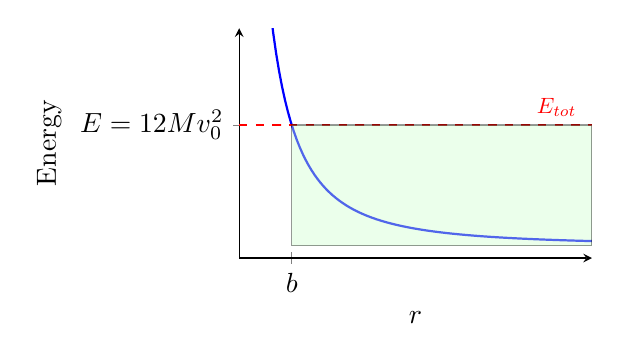
\begin{tikzpicture}
\begin{axis}[
  width=0.5\textwidth, height=4.5cm,
  xlabel={$r$}, ylabel={Energy},
  xmin=0.3, xmax=5, ymin=-0.1, ymax=1.8,
  xtick={1}, xticklabels={$b$},
  ytick={1.0}, yticklabels={$E=\tfrac{1}{2}Mv_0^2$},
  axis lines=left, samples=120,
]
  \addplot[thick,blue,domain=0.32:5]{1/(x*x)} node[pos=0.08,right,scale=0.8]{$U_\text{eff}$};
  \addplot[thick,dashed,red,domain=0.3:5]{1.0} node[pos=0.9,above,scale=0.8]{$E_\text{tot}$};
  % KE region shading
  \addplot[fill=green!20, opacity=0.4, domain=1:5] {1.0} \closedcycle;
\end{axis}
\end{tikzpicture}
\end{center}
\caption{Energy diagram for two non-interacting particles. The effective potential $U_\text{eff} = \frac{1}{2}Mv_0^2 b^2/r^2$ (blue) diverges at $r=0$. The total energy $E = \frac{1}{2}Mv_0^2$ (red dashed) is constant. The kinetic energy $KE = E - U_\text{eff}$ is non-negative; motion is restricted to $r \geq b$.}
\label{fig:eff_pot_centrifugal}
\end{figure}

Since $KE \geq 0$, $E - U_\text{eff} \geq 0$.

This whole setup is equivalent to a single particle $M$ in 1D, $\mu$, moving in $r$-space.
\end{example}

\section{Energy Diagrams and Planetary Motion}

In the context of planetary motion,
\[
  f(r) = -\frac{Gm_1 m_2}{r^2}
\]
\[
  U(\infty) - U(r) = -\int_r^\infty f(r')\,dr' = -\frac{Gm_1 m_2}{r}
\]
Thus,
\[
  U(r) = -\frac{Gm_1 m_2}{r}
\]

Thus,
\[
  U_\text{eff} = \underbrace{\frac{L^2}{2Mr^2}}_{\text{dominates at small }r} - \underbrace{\frac{Gm_1 m_2}{r}}_{\text{dominates at large }r}
\]

Thus,
\[
  E = \tfrac{1}{2}M\dot{r}^2 + \frac{L^2}{2Mr^2} - \frac{Gm_1 m_2}{r}
\]

\begin{figure}[H]
\begin{center}
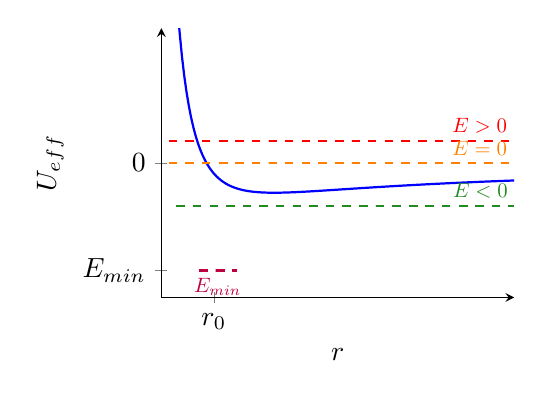
\begin{tikzpicture}
\begin{axis}[
  width=0.5\textwidth, height=5cm,
  xlabel={$r$}, ylabel={$U_\text{eff}$},
  xmin=0.3, xmax=5, ymin=-2.5, ymax=2.5,
  xtick={1.0}, xticklabels={$r_0$},
  ytick={-2.0,0}, yticklabels={$E_\text{min}$,$0$},
  axis lines=left, samples=150,
]
  % Effective potential: L^2/(2mr^2) - C/r
  \addplot[thick,blue,domain=0.42:5]{1.8/(x*x) - 2.0/x} node[pos=0.05,right,scale=0.75]{$U_\text{eff}$};
  % Horizontal energy lines
  \addplot[thick,dashed,red,domain=0.4:5]{0.4}    node[pos=0.9,above,scale=0.75]{$E>0$};
  \addplot[thick,dashed,orange,domain=0.4:5]{0.0} node[pos=0.9,above,scale=0.75]{$E=0$};
  \addplot[thick,dashed,ForestGreen,domain=0.5:5]{-0.8} node[pos=0.9,above,scale=0.75]{$E<0$};
  \addplot[thick,dashed,purple,domain=0.8:1.3]{-2.0} node[pos=0.5,below,scale=0.75]{$E_\text{min}$};
\end{axis}
\end{tikzpicture}
\end{center}
\caption{Effective potential for planetary motion $U_\text{eff}(r) = L^2/(2Mr^2) - C/r$ (blue). Four energy cases: $E>0$ (unbound, hyperbola), $E=0$ (parabola), $E<0$ (bound ellipse), and $E=E_\text{min}$ at $r=r_0$ (circular orbit).}
\label{fig:planetary_eff_pot}
\end{figure}

(See lecture notes for cases.)

\section{Perturbed Circular Orbit}

A satellite of mass $m$ orbits Earth at radius $r_0$ (changes energy of the satellite but not angular momentum) — fires thruster towards the Earth.

\[
  \frac{m_1 m_2}{m_1 + m_2} \approx \frac{m_1 m_e}{m_e} = m_1
\]

\textbf{Approximate solution:} approximate $U_\text{eff}(r)$ in the neighbourhood of $r_0$.

We know $U_\text{eff} = -\frac{C}{r} + \frac{L^2}{2mr^2}$ (since $\mu \approx m$).

\[
  \left.\frac{\partial U_\text{eff}}{\partial r}\right|_{r_0} = \frac{C}{r_0^2} - \frac{L^2}{mr_0^3} = 0
\]
\[
  \Rightarrow \quad L = \sqrt{mCr_0} \qquad (\text{where } C = GmM_E)
\]

We know
\[
  \beta = \sqrt{\frac{k}{m}} = \sqrt{\frac{\partial^2 U_\text{eff}}{\partial r^2}\cdot\frac{1}{m}} \approx \sqrt{\frac{C}{mr_0^3}} = \frac{L}{mr_0^2}
\]

Thus,
\[
  r = r_0 + A\sin(\beta t) + B\cos(\beta t)
\]
Since $r(0) = r_0$:
\[
  r = r_0 + A\sin(\beta t)
\]

\textbf{Finding the new orbit:}
\[
  \dot{\theta} = \frac{L}{mr_0^2} \quad \Rightarrow \quad \theta = \left(\frac{L}{mr_0^2}\right)t \equiv \beta t
\]

Thus,
\[
  r = r_0 + A\sin(\theta)
\]

\chapter{Planetary Motion}

\section{Planetary Motion}

\textbf{Goal:} find the orbital trajectory of a planet of mass $m$ moving about a star of mass $M$ under the gravitational interaction
\[
  U(r) = -G\frac{Mm}{r} = -\frac{C}{r}
\]

Most commonly, $C = GmM_E = mg R_E^2$ for a satellite orbiting the Earth.

Using the $\theta(r)$ equation with $U(r)$:
\[
  \boxed{\theta - \theta_0 = L\int_r \frac{dr}{\sqrt{2MEr^2 + 2MCr - L^2}}}
\]

We can solve the integral to show that
\begin{equation}
  r = \frac{L^2/MC}{1 - \sqrt{1 + (2EL^2/MC^2)}\,\sin(\theta - \theta_0)} \tag{1}
\end{equation}

where $\theta_0$ is conventionally $-\pi/2$ (why?), and
\[
  r_0 = \frac{L^2}{MC} \quad \text{(radius of circular orbit corresponding to $L$, $M$, $C$)}
\]

\begin{formula}[Eccentricity]
\[
  \epsilon \equiv \sqrt{1 + \frac{2EL^2}{MC^2}} \tag{2}
\]
called the \emph{eccentricity}.
\end{formula}

Thus, (1) becomes
\[
  r = \frac{r_0}{1 - \epsilon\cos\theta}
\]

Rewriting in Cartesian coordinates: $r = \sqrt{x^2 + y^2}$, $r\cos\theta = x$,
\begin{align*}
  &\Rightarrow \quad r - \epsilon r\cos\theta = r_0 \\
  &\Rightarrow \quad \sqrt{x^2+y^2} - \epsilon x = r_0
\end{align*}

Squaring:
\[
  r_0^2 = x^2 + y^2 - 2\sqrt{x^2+y^2}\,\epsilon x + \epsilon^2 x^2
\]
\begin{equation}
  \boxed{= (1-\epsilon^2)x^2 - 2r_0\,\epsilon\, x + y^2} \tag{3}
\end{equation}

$\Rightarrow$ is a conic section.

\section{Implications of Eccentricity}

\begin{enumerate}
  \item If $\epsilon > 1$, $E > 0$ (by (2)) $\Rightarrow$ system is unbounded, so has equation of a \textbf{hyperbola}.

  \item $\epsilon = 1 \Rightarrow E = 0$; system is on the border between bounded and unbounded.

  Thus (3) becomes
  \[
    x = \frac{y^2}{2r_0} - \frac{r_0}{2} \quad \Rightarrow \text{ equation of a \textbf{parabola}.}
  \]

  \item $0 \leq \epsilon < 1 \Rightarrow -\frac{MC^2}{2L^2} \leq E < 0$

  $\Rightarrow$ system is bounded, so the equation is of an \textbf{ellipse}.

  (If $E = -\frac{MC^2}{2L^2}$, eq.\ becomes $x^2 + y^2 = r_0^2$, eq.\ of a \textbf{circle}.)
\end{enumerate}

\section{Hyperbolic Orbits}

Examine a projectile $\mu$ with velocity $v_0$, being gravitationally attracted to the atom with \emph{impact parameter} $b$:

\begin{figure}[H]
  \centering
  \caption{Hyperbolic orbit diagram: incoming projectile $\mu$ with velocity $v_0$ and impact parameter $b$, deflected through scattering angle $\psi = \pi - 2\theta_a$. The closest approach is $r_\text{min}$.}
\end{figure}

Thus, we have:
\[
  L = \mu v_0 b \quad \text{(because $\vec{b}$ is $\perp$ to $v_0$)}
\]
\[
  E = \tfrac{1}{2}\mu v_0^2, \qquad U(r) = -C/r
\]
\[
  r = \frac{r_0}{1 - \epsilon\cos\theta} \tag{2}
\]

where
\begin{equation}
  r_0 = \frac{L^2}{MC} = \frac{\mu v_0^2 b^2}{C} = \frac{2Eb^2}{C} \tag{1}
\end{equation}

and
\[
  \epsilon = \sqrt{1 + \frac{2EL^2}{MC^2}} = \sqrt{1 + \left(\frac{2Eb}{C}\right)^2}
\]

Thus, by (1), $L^2 = 2\mu E b^2$.

When $\theta = \pi$, $r = r_\text{min}$, and by (2):
\[
  r_\text{min} = \frac{r_0}{1+\epsilon} = \frac{2Eb^2/C}{1 + \sqrt{1+(2Eb/C)^2}}
\]

Thus, as $E \to \infty$, $r_\text{min} \to b$ $\Rightarrow$ $0 < r_\text{min} < b$.

The half-angle $\theta_a$ between asymptotes, by (2), is found by letting $r \to \infty$:
\begin{equation}
  \cos(\theta_a) = \frac{1}{\epsilon} \tag{3}
\end{equation}

\subsection{Scattering Angle}

The \emph{scattering angle}: the angle that $\mu$ is deflected by ($\psi = \pi - 2\theta_a$).

Thus,
\[
  \cos(\theta_a) = \cos(\pi/2 - \psi/2) = \sin(\psi/2)
\]

So
\[
  \sin(\psi/2) = \frac{1}{\epsilon} = \frac{1}{\sqrt{1 + (2Eb/C)^2}}
\]

\section{Elliptical Orbits and Planetary Motion}

Recall that for $0 \leq \epsilon < 1$:
\[
  (1-\epsilon^2)x^2 - 2r_0\,\epsilon\, x + y^2 = r_0^2
\]

A focus of the ellipse is at the origin (the Sun).

\[
  r_\text{min} + r_\text{max} = A \quad \text{(Major axis)}
  = r_0\!\left(\frac{1}{1+\epsilon} + \frac{1}{1-\epsilon}\right)
  = \frac{2r_0}{1-\epsilon^2}
  = \frac{2L^2/\mu C}{1-(1+2EL^2/\mu C^2)}
\]
\[
  = \underbrace{\frac{C}{-E}}_{\text{independent of }L!}
\]

Thus,
\[
  E = \frac{-C}{A} = \tfrac{1}{2}\mu v_0^2 - \frac{C}{r}
\]

\begin{formula}[Vis-viva equation]
\[
  \boxed{v^2 = \frac{2C}{\mu}\!\left(\frac{1}{r} - \frac{1}{A}\right)}
\]
\emph{Orbital speed at any position $r$.}
\end{formula}

\section{Period of an Elliptic Orbit}

Recall the $r(t)$ equation:
\[
  t_b - t_a = \mu\int_{r_a}^{r_b} \frac{r\,dr}{\sqrt{2\mu Er^2 + 2\mu Cr - L^2}}
\]
(with $E < 0$). Integrating, we find that
\[
  t_b - t_a = \left.\frac{\sqrt{2\mu Er^2 + 2\mu Cr - L^2}}{2E}\right|_{r_a}^{r_b}
\]

Skipping to the result,
\[
  T = \left(\frac{\pi\mu C}{-E}\right)\frac{1}{\sqrt{-2\mu E}}
\]
\[
  T^2 = \frac{\pi^2\mu C^2}{-2E^3} = \frac{\pi^2\mu}{2C}\,A^3 \qquad \leftarrow \text{constant}
\]

\begin{formula}[Kepler's Third Law]
\[
  \boxed{T^2 \propto A^3}
\]
where $k$ is the constant of proportionality — $k$ is about the same for all planets in our solar system!
\end{formula}

\subsection{Simpler Way to Calculate Period}

\[
  L = \mu r^2 \dv{\theta}{t} \quad \Rightarrow \quad \frac{L}{2\mu}\,dt = \tfrac{1}{2}r^2\,d\theta = \text{area element in polar coordinates}
\]

\begin{figure}[H]
  \centering
  \caption{Area swept by the radius vector: the infinitesimal area element $\frac{1}{2}r^2\,d\theta$ in polar coordinates, and the ellipse with semi-axes $b$ and $r_a$.}
\end{figure}

Thus,
\[
  \frac{LT}{2\mu} = \text{area of the ellipse} = \pi ab
\]

where
\[
  a = \frac{A}{2} = \frac{C}{-2E}, \qquad b = \frac{L}{\sqrt{-2\mu E}}
\]

Thus,
\[
  T^2 = \frac{\pi^2\mu}{2C}\,A^3
\]

\section{Orbit Eccentricities}

\begin{itemize}
  \item As $\epsilon \to 0$, $\dfrac{r_\text{max}}{r_\text{min}} \to 1$ $\Rightarrow$ ellipse is roughly circular.
  \item As $\epsilon \to 1$, ellipse gets very elongated.
\end{itemize}

\begin{example}[Geostationary Orbit]
A satellite is \underline{geostationary} if its orbit is in the equatorial plane and its angular velocity $\Omega_e = $ Earth's rotation.

For satellite of mass $m$, $A = 2r$, $\mu \approx m$:
\[
  C = mgR_E^2, \qquad v = r\Omega_e
\]
\[
  v^2 = (r\Omega_e)^2 = \frac{2C}{m}\!\left(\frac{1}{r} - \frac{1}{2r}\right) = \frac{C}{rm}
\]
\[
  r^3 = \frac{gR_E^2}{\Omega_e^2}
\]
\[
  \Rightarrow \quad r = \sqrt[3]{\frac{gR_E^2}{\Omega_e^2}}
\]
\end{example}

\chapter{Non-Inertial Systems and Fictitious Forces}

\section{Non-Inertial Frames}

$\vec{F} = m\vec{a}$ holds \emph{only} for inertial frames (non-accelerating frame).

\begin{figure}[H]
  \centering
  \caption{Three observers Alice, Bob, and Charlie, each moving at different constant velocities $\vec{v}_1$, $\vec{v}_2$. In inertial frames: Charlie sees Alice at $\vec{v}_1$ and Bob at $\vec{v}_2$; Bob sees Alice at $\vec{v}_1 - \vec{v}_2$ and Charlie at $-\vec{v}_2$; Alice sees Bob at $\vec{v}_2 - \vec{v}_1$ and Charlie at $-\vec{v}_1$. $F = ma$ remains unchanged in these inertial frames.}
\end{figure}

What happens in an accelerating frame?

\section{Accelerating Frame}

If Alice is accelerating:
\[
  \vec{a}_\text{Charlie} = \vec{a}_\text{Alice} + \vec{A} \quad \text{(additional acceleration)}
\]
($\vec{a}_\text{rest}$ = acceleration of Alice according to Charlie)

\[
  \vec{a}_\text{Alice} = \vec{a}_\text{Charlie} - \vec{A}
\]
\[
  a' = a - A
\]
\[
  F_\text{Alice} = ma' = m(\vec{a} - \vec{A}) = \vec{F}_\text{rest} - mA
\]

\begin{figure}[H]
  \centering
  \caption{Left (Lab frame): pendulum of mass $m$ with tension $T$ at angle $\theta$, with gravity $mg$ downward and acceleration $\vec{A}$ of the car. Right (Accelerating frame): same pendulum with fictitious force $F_\text{fict} = mA$ pointing backward, gravity $mg$ downward.}
\end{figure}

\textbf{Lab frame equations:}
\begin{align*}
  &\text{(1)}\quad T\cos\theta - mg = 0 \\
  &\text{(2)}\quad T\sin\theta = mA \\
  &T^2\cos^2\theta + T^2\sin^2\theta = (mg)^2 + (mA)^2 \\
  &\Rightarrow \quad T = m\sqrt{g^2 + A^2}
\end{align*}

\textbf{Accelerating frame equations:}
\begin{align*}
  &T\cos\theta - mg = 0 \\
  &T\sin\theta - F_\text{fict} = 0, \quad F_\text{fict} = mA \\
  &\tan\theta = \frac{F_\text{fict}}{mg} \\
  &T = m\sqrt{g^2+A^2}
\end{align*}

$\Rightarrow$ Physical quantities stay the same regardless of which frame we are in.

\subsection{Pendulum in an Accelerating Frame}

What happens when the pendulum starts to oscillate?

\begin{figure}[H]
  \centering
  \caption{Pendulum oscillating in an accelerating car: the new equilibrium point is displaced; the apparent vertical is tilted. In the accelerating frame, apparent gravity $g'$ points at angle $\phi_0$ (combining $mg$ downward and fictitious force $mA$ backward).}
\end{figure}

\begin{itemize}
  \item Apparent gravity is at an angle $\phi_0$.
  \item The tension is also different: $T = m\sqrt{g^2 + A^2}$.
\end{itemize}

\begin{formula}[Pendulum frequency in accelerating frame]
\[
  \boxed{\omega^2 = \frac{g'}{l}}
\]
where $g' = \sqrt{g^2+A^2}$ is the effective gravitational acceleration.
\end{formula}

\section{Rotating Frames}

\subsection{Rotational Coordinates}

A rotating frame is an \underline{accelerating frame}.

\subsubsection{Rate of Change of a Rotating Vector}

Consider a vector $\vec{B}$ rotating at rate $\Omega$ about an axis in direction $\hat{n}$.

\begin{itemize}
  \item $\alpha$: angle between $\vec{B}$ and $\vec{\Omega}$
  \item $\vec{B}$ sweeps out a circular path with radius $B\sin\alpha$
\end{itemize}

Assuming the rotation is at constant $\Omega$, the change of vector $\vec{B}$ is:
\[
  \partial\vec{B} = \vec{B}(t+\Delta t) - \vec{B}(t) = B\sin\alpha\,\Omega\,\Delta\theta \approx (B\sin\alpha)\,\Omega\,\Delta t
\]

By the small-angle approximation:
\[
  \Delta B \approx 2B\sin\alpha\,\sin\!\left(\frac{\Omega\Delta t}{2}\right) \approx (B\sin\alpha)\,\Omega\,\Delta t
\]

\[
  \Rightarrow \quad \frac{\partial\vec{B}}{\partial t} = \lim_{\Delta t\to 0}\frac{B\sin\alpha\,\Omega\,\Delta t}{\Delta t} = (B\sin\alpha)\,\Omega
\]

\begin{formula}[Rate of change of a rotating vector]
\[
  \boxed{\frac{\partial\vec{B}}{\partial t} = \vec{\Omega}\times\vec{B}}
\]
Same as $\dv{\vec{r}}{t} = \vec{\omega}\times\vec{r}$ as derived earlier. Holds true for any vector that undergoes rotation around an axis at rate $\hat{n}$.
\end{formula}

\subsection{Derivative of a Rotating Vector}

Now, let's start with a vector $\vec{C}$ moving in a rotating frame. What is the speed of $\vec{C}$?

In the inertial system:
\[
  \vec{C} = C_x\hat{x} + C_y\hat{y} + C_z\hat{z}
\]

In the rotating system:
\[
  \vec{C} = C_x'\hat{x}' + C_y'\hat{y}' + C_z'\hat{z}'
\]

\[
  \frac{\partial\vec{C}}{\partial t} = \frac{\partial C_x^\text{rot}}{\partial t}\hat{x} + \frac{\partial C_y^\text{rot}}{\partial t}\hat{y} + \frac{\partial C_z^\text{rot}}{\partial t}\hat{z}
  + C_x\frac{\partial\hat{x}}{\partial t} + C_y\frac{\partial\hat{y}}{\partial t} + C_z\frac{\partial\hat{z}}{\partial t}
\]

Given that $\dfrac{\partial\hat{x}}{\partial t} = \vec{\Omega}\times\hat{x}$ (due to rotating in a rotating frame!),

\begin{formula}[Time derivative in rotating frame]
\[
  \frac{\partial\vec{C}}{\partial t} = \left(\frac{\partial\vec{C}}{\partial t}\right)^\text{in frame} + \vec{\Omega}\times\vec{C}
\]
\end{formula}

The non-inertial terms are:
\[
  C_x(\vec{\Omega}\times\hat{x}') + C_y(\vec{\Omega}\times\hat{y}') + C_z(\vec{\Omega}\times\hat{z}') = \vec{\Omega}\times(C_x'\hat{x}' + C_y'\hat{y}' + C_z'\hat{z}') = \vec{\Omega}\times\vec{C}
\]

Think of it as an operator:
\[
  \left(\frac{d}{dt}\right)_\text{in} = \left(\frac{d}{dt}\right)_\text{rot} + \vec{\Omega}\times
\]

\section{Velocity and Acceleration in a Rotating Frame}

For position, we have:
\[
  \left(\frac{\partial\vec{r}}{\partial t}\right)_\text{in} = \left(\frac{\partial\vec{r}}{\partial t}\right)_\text{rot} + \vec{\Omega}\times\vec{r}
\]
\[
  \Rightarrow \quad \vec{v}_\text{in} = \vec{v}_\text{rot} + \vec{\Omega}\times\vec{r}
\]

Taking the derivative of this expression:
\[
  \vec{a}_\text{in} = \vec{a}_\text{rot} + 2\vec{\Omega}\times\vec{v}_\text{rot} + \vec{\Omega}\times(\vec{\Omega}\times\vec{r})
\]

The full derivation:
\[
  \left(\frac{\partial\vec{v}_\text{in}}{\partial t}\right)_\text{in}
  = \left[\frac{\partial}{\partial t}\!\left(\vec{v}_\text{rot} + \vec{\Omega}\times\vec{r}\right)\right]_\text{rot} + \vec{\Omega}\times\!\left(\vec{v}_\text{rot} + \vec{\Omega}\times\vec{r}\right)
\]
\[
  = \left(\frac{\partial\vec{v}_\text{rot}}{\partial t}\right)_\text{rot} + \vec{\Omega}\times\!\left(\frac{\partial\vec{r}}{\partial t}\right) + \vec{\Omega}\times\!\left(\vec{v}_\text{rot} + \vec{\Omega}\times\vec{r}\right)
\]
\[
  \frac{\partial\vec{v}_\text{in}}{\partial t} = \left(\frac{\partial\vec{v}_\text{rot}}{\partial t}\right)_\text{rot} + 2\vec{\Omega}\times\vec{v}_\text{rot} + \vec{\Omega}\times(\vec{\Omega}\times\vec{r})
\]

\begin{formula}[Acceleration in terms of frames]
\[
  \boxed{\underbrace{\vec{a}_\text{in}}_{\text{inertial frame}} = \vec{a}_\text{rot} + 2\vec{\Omega}\times\vec{v}_\text{rot} + \vec{\Omega}\times\!\left(\vec{\Omega}\times\vec{r}\right)}
\]
\end{formula}

\section{Fictitious Forces in a Rotating Coordinate System}

In the rotating frame, $\vec{F}_\text{rot} = m\vec{a}_\text{rot}$:

\begin{formula}[Fictitious forces in rotating frame]
\[
  \vec{F}_\text{rot} = m\vec{a}_\text{in} - \underbrace{2m\vec{\Omega}\times\vec{v}_\text{rot}}_{\text{Coriolis force}} - \underbrace{m\vec{\Omega}\times(\vec{\Omega}\times\vec{r})}_{\text{Centrifugal force}}
\]
\end{formula}

Let $\vec{\Omega} = \Omega\hat{z}$. In spherical coordinates ($\hat{z}$, $\hat{r}$, $\hat{\theta}$):
\[
  \vec{\Omega} = \Omega\hat{z}
\]
\[
  \vec{r} = r\sin\alpha\,\hat{\rho} + r\cos\alpha\,\hat{z}
\]
\[
  \vec{\Omega}\times\vec{r} = \Omega\,r\sin\alpha\,(\hat{z}\times\hat{\rho}) = \Omega\,r\sin\alpha\,\hat{\theta}
\]

\[
  \vec{\Omega}\times(\vec{\Omega}\times\vec{r}) = \vec{\Omega}\times(\Omega\,r\sin\alpha\,\hat{\theta})
  = \Omega^2 r\sin\alpha\,(\hat{z}\times\hat{\theta})
  = -\Omega^2 r\sin\alpha\,\hat{\rho}
\]

\begin{example}[Falling Object in a Rotating Frame]
\begin{figure}[H]
  \centering
  \caption{A mass $m$ falling near the surface of the rotating Earth (depicted as a circle with rotation $\Omega$).}
\end{figure}
\end{example}

\chapter{Non-Inertial Systems: Rotating Coordinates (9.1--9.5)}

\section{Rate of Change of a Rotating Vector}

\begin{itemize}
  \item Consider a vector $\vec{B}$ that is rotating at rate $\Omega$ about an axis in direction $\hat{n}$.
  \item $\alpha$: angle between $\vec{B}$ and $\vec{\Omega}$.
  \item $\vec{B}$ sweeps out a circular path with radius $B\sin\alpha$.
\end{itemize}

By the small-angle approximation:
\[
  \Delta B = 2B\sin\alpha\,\sin\!\left(\frac{\Omega\Delta t}{2}\right) \approx (B\sin\alpha)\,\Omega\,\Delta t
\]

\[
  \Rightarrow \quad \frac{\partial\vec{B}}{\partial t} = \lim_{\Delta t\to 0}\frac{B\sin\alpha\,\Omega\,\Delta t}{\Delta t} = (B\sin\alpha)\,\Omega = \vec{\Omega}\times\vec{B} = \frac{\partial\vec{B}}{\partial t}
\]

Holds true for any vector that undergoes rotation around an axis at rate $\hat{n}$.

\section{Time Derivative of a Vector in a Rotating Coordinate System}

Consider any vector $\vec{C}$ changing at rate $\left(\dfrac{\partial\vec{C}}{\partial t}\right)_\text{in}$ as observed in an inertial system. (We are not rotating.)

Problem: find the time derivative $\left(\dfrac{\partial\vec{C}}{\partial t}\right)_\text{rot}$ in a rotating coordinate system.

In the inertial system:
\[
  \vec{C} = C_x\hat{i} + C_y\hat{j} + C_z\hat{k}
\]

In the rotating system:
\[
  \vec{C} = C_x'\hat{i}' + C_y'\hat{j}' + C_z'\hat{k}'
\]

But by the previous result:
\[
  \frac{\partial\hat{i}'}{\partial t} = \vec{\Omega}\times\hat{i}', \quad
  \frac{\partial\hat{j}'}{\partial t} = \vec{\Omega}\times\hat{j}', \quad
  \frac{\partial\hat{k}'}{\partial t} = \vec{\Omega}\times\hat{k}' \qquad \text{(Non-inertial terms)}
\]

Thus,
\[
  \left(\frac{\partial\vec{C}}{\partial t}\right)_\text{rot} = \left(\frac{\partial C_x'}{\partial t}\hat{i}' + \frac{\partial C_y'}{\partial t}\hat{j}' + \frac{\partial C_z'}{\partial t}\hat{k}'\right)
  + \left(C_x'\frac{\partial\hat{i}'}{\partial t} + C_y'\frac{\partial\hat{j}'}{\partial t} + C_z'\frac{\partial\hat{k}'}{\partial t}\right)
\]

The second bracket equals:
\[
  C_x'(\vec{\Omega}\times\hat{i}') + C_y'(\vec{\Omega}\times\hat{j}') + C_z'(\vec{\Omega}\times\hat{k}') = \vec{\Omega}\times(C_x'\hat{i}' + C_y'\hat{j}' + C_z'\hat{k}') = \vec{\Omega}\times\vec{C}
\]

\[
  \Rightarrow \quad \boxed{\left(\frac{\partial\vec{C}}{\partial t}\right)_\text{in} = \left(\frac{\partial\vec{C}}{\partial t}\right)_\text{rot} + \vec{\Omega}\times\vec{C}}
\]

Think of it as an operator:
\[
  \left(\frac{d}{dt}\right)_\text{in} = \left(\frac{d}{dt}\right)_\text{rot} + \vec{\Omega}\times
\]

\section{Velocity and Acceleration in a Rotating Coordinate System}

For position, we have:
\[
  \left(\frac{\partial\vec{r}}{\partial t}\right)_\text{in} = \left(\frac{\partial\vec{r}}{\partial t}\right)_\text{rot} + \vec{\Omega}\times\vec{r}
\]
\[
  \Rightarrow \quad \vec{v}_\text{in} = \vec{v}_\text{rot} + \vec{\Omega}\times\vec{r}
\]

Taking the derivative of this expression:
\[
  \vec{a}_\text{in} = \vec{a}_\text{rot} + 2\vec{\Omega}\times\vec{v}_\text{rot} + \vec{\Omega}\times(\vec{\Omega}\times\vec{r})
\]

\subsection{Fictitious Forces}

Thus, $m\vec{a}_\text{in} = \vec{F}_m$:
\[
  \vec{F}_\text{rot} = \vec{F}_\text{in} - \underbrace{2m\vec{\Omega}\times\vec{v}_\text{rot}}_{\text{Coriolis}} - \underbrace{m\vec{\Omega}\times(\vec{\Omega}\times\vec{r})}_{\substack{\text{Centrifugal}\\F_c = -m\vec{\Omega}\times(\vec{\Omega}\times\vec{r})}}
\]

\begin{itemize}
  \item Centrifugal force magnitude: $m\Omega^2\rho$ (where $\rho$ is the perpendicular distance from the axis of rotation to the tip of $\vec{r}$).
  \item Coriolis: fictitious force to balance the Coriolis acceleration $2\vec{\Omega}\times\vec{v}_\text{rot}$.
  \item Coriolis magnitude: $2m\dot{r}\omega$ (for $v_\rho$) or $2mr\dot{\theta}\omega$ (for $v_\theta$).
\end{itemize}

\textbf{Important:} $\vec{v}_\text{rot}$ is velocity in the \emph{rotating} frame, not the inertial frame!

\begin{fact}[Horizontal Coriolis force]
\[
  \vec{F}_H = -2m\Omega\sin\lambda\,(\hat{r}\times\vec{v}) \qquad \text{(horizontal component)}
\]
\end{fact}

\begin{example}[Surface of a Rotating Liquid]
\begin{figure}[H]
  \centering
  \caption{Rotating liquid bucket: in the rotating frame, forces on a fluid element are normal force $F_\text{norm}$, centrifugal force $m\omega^2 r$ outward, and gravity $W = mg$ downward. The surface tilts so that $\phi = \tan^{-1}(\omega^2 r / g)$.}
\end{figure}

Equations of equilibrium in the rotating frame:
\[
  F_0\cos\phi - W = 0
\]
\[
  -F_0\sin\phi + F_\text{cent} = 0
\]
\[
  \Rightarrow \quad F_\text{cent} = m\Omega^2 r = m\omega^2 r \quad (\text{since } \Omega = \omega \text{ for a coordinate system with rotating bucket})
\]

\begin{formula}[Shape of rotating liquid surface]
\[
  \phi = \tan^{-1}\!\left(\frac{\omega^2 r}{g}\right) \qquad \text{important tool!}
\]
\[
  \boxed{\frac{dz}{dr} = \tan\phi = \frac{\omega^2 r}{g}}
\]
\end{formula}

Integrating:
\[
  \int dz = \frac{\omega^2}{g}\int r\,dr = \tfrac{1}{2}\frac{\omega^2}{g}r^2
\]

The surface is a paraboloid $z = \dfrac{\omega^2}{2g}r^2$.
\end{example}

\begin{example}[Sliding Bead and Coriolis Forces]
A bead slides without friction on a horizontal wire. Find the force exerted on the bead by the wire.

\begin{figure}[H]
  \centering
  \caption{Bead on a horizontal rotating wire: in the rotating frame, the bead at distance $r$ experiences centrifugal force $F_\text{cent}$ outward and Coriolis (normal) force $N$ perpendicular to the wire.}
\end{figure}

Equations of motion:
\[
  F_\text{cent} = m\ddot{r}, \qquad N - F_\text{Cor} = 0 \quad \Rightarrow \quad N = F_\text{Cor}
\]
\[
  F_\text{cent} = m\omega^2 r \quad \Rightarrow \quad m\ddot{r} = m\omega^2 r
\]

which has solution $r = Ae^{\omega t} + Be^{-\omega t}$.

(The Coriolis force $F_\text{Cor}$ is found similarly.)
\end{example}

\begin{example}[Deflection of a Falling Mass]

\begin{figure}[H]
  \centering
  \caption{Mass $m$ falling near the rotating Earth (rotation $\Omega$), with motion confined to the equatorial plane. The coordinates $\hat{r}$ (radial) and $\hat{\theta}$ (tangential) are shown.}
\end{figure}

\[
  \vec{F} = -mg\hat{r} - 2m\vec{\Omega}\times\vec{v}_\text{rot} - m\vec{\Omega}\times(\vec{\Omega}\times\vec{r})
\]

Motion is confined to the equatorial plane:
\[
  \vec{v}_\text{rot} = \dot{r}\hat{r} + r\dot{\theta}\hat{\theta}
\]
\[
  \vec{\Omega}\times\vec{v}_\text{rot} = \Omega\dot{r}\hat{\theta} - r\Omega\dot{\theta}\hat{r}, \qquad \vec{\Omega}\times(\vec{\Omega}\times\vec{r}) = \Omega^2 r\hat{r}
\]

\textit{Tip: this doesn't change that the $\hat{r}$, $\hat{\theta}$ equations of motion still apply.}

\[
  \vec{F}_\text{rot} = -mg\hat{r} - 2m(\Omega\dot{r}\hat{\theta} - r\Omega\dot{\theta}\hat{r}) - mr\Omega^2\hat{r}
\]
\[
  \vec{F}_\text{rad} = -mg\hat{r} + 2mr\Omega\dot{\theta}\hat{r} - mr\Omega^2\hat{r}
\]
\[
  \vec{F}_\text{tan} = -2m\Omega\dot{r}\hat{\theta} = mr\ddot{\theta}
\]

We can omit terms with $\dot{\theta}$ because $m$ falls approximately vertically:
\[
  \ddot{r} \approx -g + \Omega^2 r
\]
\[
  r\ddot{\theta} \approx -2\dot{r}\Omega
\]

We can also take $r \approx R_E$, and let $g$ be constant:
\[
  \Rightarrow \quad \ddot{r} \approx -g' \quad \text{where } g' = g - \Omega^2 R_E
\]

Thus,
\[
  \dot{r} = -g't, \qquad r = r_0 - \tfrac{1}{2}g't^2
\]

\[
  r\ddot{\theta} = 2g't\Omega \quad \Rightarrow \quad \dot{\theta} = \frac{g't^2\Omega}{R_E}
\]
\[
  \Rightarrow \quad \dot{\theta} = \frac{g\Omega}{R_E}t^2
\]
\[
  \Rightarrow \quad \theta = \frac{1}{2}\frac{g\Omega}{R_E}t^3
\]

Thus, the horizontal deflection of $m$ is:
\[
  y \approx R_E\theta \approx \tfrac{1}{3}g\Omega t^3
\]

Time $T$ to fall a distance $h$ is given by:
\[
  r - r_0 = -h = -\tfrac{1}{2}g't^2 \quad \Rightarrow \quad T = \sqrt{\frac{2h}{g}}
\]
\[
  y = \tfrac{1}{2}g\Omega\!\left(\frac{2h}{g}\right)^{3/2}
\]
\end{example}

\begin{example}[Motion on the Rotating Earth]

\[
  \vec{F}_\text{Cor} = -2m(\vec{\Omega}\times\vec{v})
\]

\begin{figure}[H]
  \centering
  \caption{The rotating Earth with rotation $\vec{\Omega}$, showing decomposition of $\vec{\Omega}$ into vertical ($\Omega_V$) and horizontal ($\Omega_H$) components at latitude $\lambda$.}
\end{figure}

\begin{itemize}
  \item Consider a velocity $\vec{v}$ transverse to the rotation.
  \item Horizontal component of Coriolis force is $\perp$ to $\vec{v}$ and its magnitude is independent of direction of $\vec{v}$.
\end{itemize}

Thus,
\begin{align*}
  \vec{F} &= -2m(\vec{\Omega}\times\vec{v}) \\
  &= -2m(-\Omega_V\times\vec{v} + \Omega_H\times\vec{v}) \\
  &= \vec{F}_V + \vec{F}_H \quad ?
\end{align*}
\end{example}

\chapter{Morin Chapter 2 Problems}

\begin{example}[2.1 --- Hanging Chain Tension]
A chain of uniform linear mass density $\rho$ and length $L$ hangs vertically ($\rho L = m$).

\begin{figure}[H]
  \centering
  \caption{Hanging chain of length $L$: at height $y$ from the bottom, a segment of length $y$ has weight $\rho y g$, requiring tension $T(y)$.}
\end{figure}

At point $y$, it is being held up by tension $T(y)$ and pulled down by gravity $\rho y g$:
\[
  T(y) - \rho y g = 0
\]
\[
  \Rightarrow \quad \boxed{T(y) = \rho g y}
\]
\end{example}

\begin{example}[2.3 --- Motionless Chain]
A chain of linear mass density $\rho$ lies at rest on an inclined plane at angle $\theta$.

\begin{figure}[H]
  \centering
  \caption{Chain element $\Delta\ell$ on an incline: the component of gravity along the slope is $\Delta F = g\sin\theta\,dm$, with $\sin\theta = \Delta y/\sqrt{\Delta x^2+\Delta y^2}$ and $\Delta\ell = \sqrt{\Delta x^2+\Delta y^2}$.}
\end{figure}

\[
  \Delta F = g\sin\theta\cdot dm = g\sin\theta\cdot\rho\,\Delta\ell, \qquad
  \sin\theta = \frac{\Delta y}{\sqrt{\Delta x^2+\Delta y^2}}, \quad \Delta\ell = \sqrt{\Delta x^2+\Delta y^2}
\]

\[
  \Rightarrow \quad \Delta F = g\frac{\Delta y}{\sqrt{\Delta x^2+\Delta y^2}}\cdot\rho\sqrt{\Delta x^2+\Delta y^2}
\]
\[
  \Rightarrow \quad \Delta F = \rho g\,\Delta y
\]

\[
  F = \int dF = \rho g\int_{y_0}^{y_1} dy = \rho g(y_0 - y_1) = 0
\]
\[
  \boxed{F_\text{net} = 0}
\]

(The net gravitational force along the slope is zero for a chain between two points at the same height, regardless of the shape of the path.)
\end{example}

\begin{example}[2.4 --- Minimum Force to Keep a Book Up]
A book of mass $M$ is pushed against a wall with a force $F$ at angle $\theta$, with friction coefficient $\mu$.

\begin{figure}[H]
  \centering
  \caption{Book against wall: applied force $F$ at angle $\theta$, normal force $N$ from wall (horizontal), friction $f$ upward along wall.}
\end{figure}

Equations:
\begin{align*}
  &\text{(1)}\quad F\cos\theta = N \\
  &\text{(2)}\quad F\sin\theta + f = Mg \\
  &\text{(3)}\quad f \leq \mu N
\end{align*}

From (1) and (3): $f \leq \mu F\cos\theta$.

From (2): $F\sin\theta + \mu F\cos\theta \geq Mg$, so $F(\sin\theta + \mu\cos\theta) \geq Mg$:
\[
  \boxed{F \geq \frac{Mg}{\sin\theta + \mu\cos\theta}} \qquad \text{assuming } \sin\theta + \mu\cos\theta > 0
\]

To minimize $F$, set $\dfrac{dF}{d\theta} = 0$:
\[
  \frac{dF}{d\theta} = \frac{-Mg}{(\sin\theta+\mu\cos\theta)^2}(\cos\theta - \mu\sin\theta) = 0
\]
\[
  \cos\theta - \mu\sin\theta = 0 \quad \Rightarrow \quad \boxed{\tan\theta = \frac{1}{\mu}}
\]

\begin{figure}[H]
  \centering
  \caption{Right triangle: opposite side $1$, adjacent side $\mu$, hypotenuse $\sqrt{1+\mu^2}$.}
\end{figure}

\[
  F \geq \frac{Mg}{\dfrac{\cos\theta}{\mu}+\mu\cos\theta} = \frac{Mg\mu}{(1+\mu^2)\cos\theta} = \frac{Mg}{(1+\mu^2)}\cdot\frac{1}{\sin\theta} = \frac{Mg}{\sqrt{1+\mu^2}}
\]

\[
  \boxed{F_\text{min} = \frac{Mg}{\sqrt{1+\mu^2}}}
\]

\textbf{Part (c):} If $\sin\theta = -\mu\cos\theta \Rightarrow \tan\theta = -\mu$:
\[
  \theta = -\tan^{-1}(\mu); \text{ if } \theta < -\tan^{-1}(\mu) \text{ then it is impossible to keep the book up.}
\]
\end{example}

\begin{example}[2.5 --- Rope on a Plane]

\textbf{Case 1:} A rope of linear density $\rho$ lies on an inclined plane at angle $\theta$, with friction coefficient $\mu$. Find the maximum tension distribution.

\begin{figure}[H]
  \centering
  \caption{Element $dm$ of rope on incline: tension $T(x)$ at left end, $T(x+dx)$ at right end, normal force $N$, friction $f$, and component of gravity $\rho\,dx\cdot g\sin\theta$ along the slope.}
\end{figure}

Equations:
\begin{align*}
  &\text{(1)}\quad T(x) + f = \rho\,dx\cdot g\sin\theta + T(x+dx) \\
  &\text{(2)}\quad f \leq \mu N = \mu\,\rho\,dx\,g\cos\theta
\end{align*}

Combining:
\[
  \mu\,\rho\,dx\,g\cos\theta \geq \rho\,dx\,g\sin\theta + T(x+dx) - T(x)
\]
\[
  \rho\,dx\,g(\mu\cos\theta - \sin\theta) \geq T(x+dx) - T(x)
\]
\[
  \frac{dT}{dx} \leq \rho g(\mu\cos\theta - \sin\theta)
\]
\[
  T(x) \leq \rho g x(\mu\cos\theta - \sin\theta)
\]
\end{example}

\section{Galilean Transformation}

Used to transfer between frames going at different velocities (but parallel axes though).

\begin{figure}[H]
  \centering
  \caption{Two frames: frame $A$ with position $\vec{r}_A$ and frame $B$ displaced by $\vec{S}$, with $\vec{r}_B = \vec{r}_A - \vec{S}$.}
\end{figure}

We have that
\begin{equation}
  \vec{r}_B = \vec{r}_A - \vec{S} \tag{1}
\end{equation}

Suppose that the mass accelerates at:
\begin{itemize}
  \item Alice: $\vec{F}_a = m\vec{a}_a$
  \item Bob observes $\vec{F}_B = M\vec{a}_B$ \quad -- are they the same?
\end{itemize}

By differentiating (1), we get:
\[
  \vec{v}_B = \vec{v}_A - \vec{V} \quad \Bigg\} \text{ Galilean transformation}
\]
\[
  \vec{a}_B = \vec{a}_A - \vec{A}
\]

If $S = $ const or $\vec{v} = $ const $\Rightarrow \vec{A} = \vec{0}$:
\[
  \vec{a}_B = \vec{a}_A \quad \Rightarrow \quad \vec{F}_B = \vec{F}_A
\]

\textbf{Assumptions:}
\begin{itemize}
  \item Lengths are measured the same (not true due to special relativity).
  \item Also time is not the same due to $g$.
\end{itemize}

\subsection{Principle of Relativity}

\textbf{Conclusion:} Laws of physics are the same in all inertial reference frames!

\section{Uniformly-Accelerating Systems}

How physics appears to an observer in a system accelerating at a constant rate $A$:
\[
  \vec{a}' = \vec{a} - \vec{A} \qquad (\text{system acceleration})
\]
(acceleration w.r.t. accelerating frame = acceleration to rest frame minus system acceleration)

\textbf{Apparent Force:}
\[
  \vec{F}' = m\vec{a}' = m\vec{a} - m\vec{A} = \vec{F} + \underbrace{\vec{F}_\text{fict}}_{= -m\vec{A}}
\]

\begin{example}[Apparent Force of Gravity]

\begin{figure}[H]
  \centering
  \caption{Pendulum in an accelerating car (acceleration $A$ to the right). Goal: find the motion.}
\end{figure}

\textbf{Laboratory system:}
\begin{align*}
  &T\sin\theta = mA \\
  &T\cos\theta = mg \\
  &\tan\theta = \frac{A}{g} \\
  &T^2 = m^2(A^2+g^2) \\
  &T = m\sqrt{A^2+g^2}
\end{align*}

\textbf{Accelerating system} ($F_\text{net} = ma = 0$):
\begin{align*}
  &T\cos\theta - W = 0 \\
  &T\sin\theta - F_\text{fict} = T\sin\theta - mA = 0 \\
  &\tan\theta = \frac{A}{g} \\
  &\Rightarrow \quad T = m\sqrt{A^2+g^2}
\end{align*}
\end{example}

\begin{example}[Cylinder on an Accelerating Plank]
A cylinder of radius $R$, mass $M$ sits on a plank that accelerates at rate $A$. No slip condition.

\begin{figure}[H]
  \centering
  \caption{Cylinder (radius $R$, mass $M$) on an accelerating plank (acceleration $A$): friction force $f$ acts on the cylinder, and a fictitious force $F_\text{fict} = mA$ acts backward in the accelerating frame.}
\end{figure}

In the accelerating frame:
\[
  f - \vec{F}_\text{fict} = ma', \qquad \text{no slip} \Rightarrow Rf = -I\alpha' = -\frac{Ia'}{R}
\]

Thus, $f = -\dfrac{Ia'}{R^2}$:
\[
  -\frac{Ia'}{R^2} - F_\text{fict} = ma'
\]
\[
  \Rightarrow \quad a' = \frac{F_\text{fict}}{M + \frac{I_0}{R^2}} = -\frac{2}{3}A
\]

Thus,
\[
  a = a' + A = \boxed{\frac{1}{3}A}
\]
\end{example}

\begin{example}[Pendulum in an Accelerating Car]
\begin{figure}[H]
  \centering
  \caption{Pendulum in accelerating car: equilibrium angle shifts to $\phi_0$; the full oscillation amplitude is $\phi = 2\phi_0 = 2J$.}
\end{figure}

Since we already know:
\[
  \phi_0 = \tan^{-1}\!\left(\frac{A}{g}\right), \qquad \phi = 2\phi_0 = 2J
\]
\end{example}

\section{Principle of Equivalence}

\begin{itemize}
  \item Laws of physics are the same in a uniformly accelerating system as long as we add a fictitious force $\vec{F}_\text{fict} = -m\vec{A}$.
  \item $\vec{F}_\text{fict}$ is indistinguishable from the force due to a uniform gravitational field $\vec{g} = -\vec{A}$.
  \item A particle in deep space free of any physical interactions but uniformly accelerating at $\vec{A} = -g$, it experiences fictitious force $\vec{F}_\text{fict} = -m\vec{A} = m\vec{g}$.
\end{itemize}

\begin{example}[Elevator Thought Experiment]

\textbf{Situation 1:} Person in a box on Earth, gravity $g$ downward.

\textbf{Situation 2:} Person in a box in deep space, box accelerating upward at $a = g$.

If the man drops the apple in both situations, they both appear to accelerate downward at rate $g$ relative to the man.

However, one might conclude that they are in a uniform gravitational field throughout all of space --- unphysical thought!

\begin{formula}[Principle of Equivalence]
No way to locally distinguish between a uniform gravitational acceleration $\vec{g}$ and an acceleration of the coordinate system $\vec{A} = -\vec{g}$.

(Locally means from within a sufficiently-defined system) --- to distinguish, you need a third reference point for plausible denial.
\end{formula}
\end{example}

\begin{example}[Driving Force of the Tides]
According to the principle of equivalence, it is impossible to observe the Sun's gravitational force on an Earth-bound system.

However, the Earth is so large it has non-local effects.
\begin{itemize}
  \item Tides due to the Sun and Moon creating an apparent gravitational field.
\end{itemize}

At the Earth's center A:
\[
  \vec{G}_0 = \frac{GM_s}{r_s^2}\hat{n}
\]

Earth accelerates toward the Sun at rate $A = G_0$.

Let $G(r)$ be the gravitational field at some point $r$ on the Earth. Then $\vec{F} = mG(r)$.

To an Earth-bound observer the force $F' = \vec{F} - m\vec{A}$:
\[
  = mG(r) - mG_0
\]

The apparent field is thus:
\[
  \frac{F'}{m} = G'(r) = G(r) - G_0
\]

\begin{figure}[H]
  \centering
  \caption{Left: Sun and Earth with gravitational fields $G_A$, $G_B$, $G_C$, $G_D$, $G_E$ at various points on the Earth (center A, near-side B, far-side C, top D, bottom E), with Earth-Sun distance $r_s$. Right: residual (tidal) fields $G_A' = 0$, $G_B'$ pointing toward Sun, $G_C'$ pointing away, $G_D'$ and $G_E'$ pointing inward (neglecting higher-order terms).}
\end{figure}

\[
  G_A' = G_A - G_0 = \frac{GM_s}{(r_s - R_E)^2} - G_0 \approx 2G_0\frac{R_E}{r_s}
\]

$G_C'$ is similar: $= -2G_0\dfrac{R_E}{r_s}$.

Using small-angle approximation: $G_D'/G_E' \approx \dfrac{1}{2}G_0\dfrac{R_E}{r_s}$ (approximately inward).
\end{example}

% Pages 174–200: Morin 2.6, Introduction to Lagrangian Mechanics,
% Calculus of Variations, Particle Interactions, Symmetry & Noether's Theorem,
% Non-Inertial Reference Frames, Double Pendulum

\chapter{Introduction to Lagrangian Mechanics}

% -----------------------------------------------------------------------
\section{Morin Problem 2.6 (Rope over a Pulley)}

A small element of rope subtending an angle $d\theta$ at angular position $\theta$
is acted on by tension forces $T(\theta + d\theta/2)$ and $T(\theta - d\theta/2)$
and a normal force $dN$ directed toward the center of the pulley.

\begin{figure}[H]
    \centering
    \caption{Rope element on a circular pulley. The element subtends angle $d\theta$;
    tension acts at $\pm d\theta/2$ from the element centre and a normal force $dN$
    acts radially inward.}
\end{figure}

Horizontal (tangential) equilibrium gives
\[
    T\!\left(\theta + \tfrac{d\theta}{2}\right)\cos\!\left(\tfrac{d\theta}{2}\right)
    =
    T\!\left(\theta - \tfrac{d\theta}{2}\right)\cos\!\left(\tfrac{d\theta}{2}\right).
\]

The vertical (normal) component of the net tension is
\[
    dN_y = 2T\sin\!\left(\tfrac{d\theta}{2}\right)\cos\theta = T\cos\theta\,d\theta.
\]

Boundary conditions: $dN_y = 0$ when $\theta = \tfrac{\pi}{2}, -\tfrac{\pi}{2}$.

Integrating,
\[
    N_y = T(\sin\theta_f - \sin\theta_i) = 2T.
\]

But $N_y = Mg$, so
\[
    \boxed{T = \frac{Mg}{2}.}
\]

\textit{Easier way:} $Mg = 2T$.  The normal force per unit length is the same
everywhere:
\[
    dN = N\,d\theta = 2T\sin\!\left(\tfrac{d\theta}{2}\right) = T\,d\theta.
\]

Since the $N\,d\theta/dN$ segment has arc length $R\,d\theta$,
\[
    \boxed{\frac{N}{R} = \frac{T}{R} = \frac{Mg}{2R}.}
\]

\subsection*{Part (b)}

Use the result that $T(\theta) \leq T(0)\,e^{\mu\theta}$.

% -----------------------------------------------------------------------
\section{Motivation}

\textit{(Lecture: Introduction to Lagrangian Mechanics, Monday January 6, 2025)}

\subsection{Newtonian Picture}

Given initial conditions $\vec{x}(t=0)$ and $\dot{\vec{x}}(t=0)$, Newton's laws
tell you how to update the system:
\[
    \vec{a} \;\to\; \vec{v} \;\to\; \vec{x}, \qquad m\ddot{\vec{x}} = \sum_i \vec{F}_i.
\]

\begin{itemize}
    \item Q: Where do Newton's laws come from? Why are certain quantities conserved?
\end{itemize}

\subsection{Motivation: Refraction and Fermat's Principle}

How does light know which path to take through a block?

\begin{itemize}
    \item \textbf{Fermat's Principle:} The path that takes the least time is the one
        that light chooses to take.
\end{itemize}

\begin{figure}[H]
\begin{center}
\begin{tikzpicture}[scale=1.0, >=Stealth]
  % Interface
  \draw[thick,dashed] (-1.5,0) -- (3.0,0);
  % Media labels
  \node[above left] at (-1.0,0.8) {$n_1$ (medium 1)};
  \node[below left] at (-1.0,-0.5) {$n_2$ (medium 2)};
  % Fill media
  \fill[blue!8] (-1.5,0) rectangle (3.0,2.0);
  \fill[orange!8] (-1.5,-1.5) rectangle (3.0,0);
  % Incident ray
  \draw[->,thick,blue] (-1.0,1.8) -- (1.0,0);
  % Refracted ray
  \draw[->,thick,red] (1.0,0) -- (2.5,-1.3);
  % Normal line
  \draw[dashed,gray] (1.0,1.5) -- (1.0,-1.2);
  % Angle theta1
  \draw (1.0,0.7) arc[start angle=90,end angle=118,radius=0.7];
  \node[left,scale=0.85] at (0.7,0.85) {$\theta_1$};
  % Angle theta2
  \draw (1.0,-0.6) arc[start angle=270,end angle=302,radius=0.6];
  \node[right,scale=0.85] at (1.2,-0.7) {$\theta_2$};
  % Snell label
  \node[right] at (2.6,-0.4) {$n_1\sin\theta_1 = n_2\sin\theta_2$};
\end{tikzpicture}
\end{center}
\caption{Snell's law from Fermat's principle: light refracts at the interface between media with speeds $v_1 = c/n_1$ and $v_2 = c/n_2$. The path of least time gives $n_1\sin\theta_1 = n_2\sin\theta_2$.}
\label{fig:fermat_snell}
\end{figure}

Is there some quantity that is optimised?

\subsection{Hamilton's Picture}

Assume we know the position at an initial and final time.  Is there a principle
that allows you to discern the path?

\begin{figure}[H]
\begin{center}
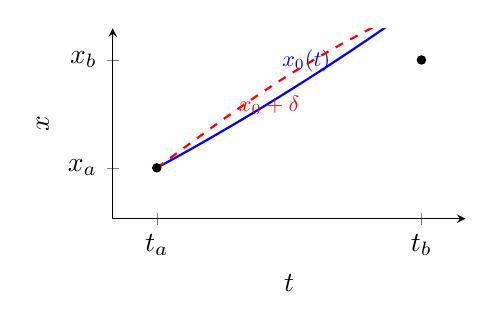
\begin{tikzpicture}
\begin{axis}[
  width=0.5\textwidth, height=4cm,
  xlabel={$t$}, ylabel={$x$},
  xmin=0, xmax=4, ymin=0, ymax=3,
  xtick={0.5,3.5}, xticklabels={$t_a$,$t_b$},
  ytick={0.8,2.5}, yticklabels={$x_a$,$x_b$},
  axis lines=left,
]
  % True path (parabola)
  \addplot[thick,blue,domain=0.5:3.5,samples=50]
    {0.8 + 0.75*(x-0.5) + 0.04*(x-0.5)^2} node[pos=0.55,above,scale=0.8]{$x_0(t)$};
  % Varied path (different curve)
  \addplot[thick,dashed,red,domain=0.5:3.5,samples=50]
    {0.8 + 0.75*(x-0.5) + 0.04*(x-0.5)^2 + 0.25*sin(deg(pi*(x-0.5)/3))}
    node[pos=0.45,below,scale=0.8]{$x_0+\delta$};
  % Endpoint marks
  \addplot[only marks,mark=*,mark size=1.5pt] coordinates {(0.5,0.8)(3.5,2.5)};
\end{axis}
\end{tikzpicture}
\end{center}
\caption{The true (classical) path $x_0(t)$ (blue solid) and a varied path $x_0(t)+\delta(t)$ (red dashed) between fixed endpoints $(t_a,x_a)$ and $(t_b,x_b)$. Hamilton's principle states $\delta S = 0$ for the true path.}
\label{fig:action_paths}
\end{figure}

% -----------------------------------------------------------------------
\section{First Principles}

\begin{enumerate}
    \item Inertial reference frames exist, and in them the CoM of an isolated system
        experiences no acceleration \textit{(1st Law)}.
    \item Space-time is homogeneous and isotropic — the fundamental laws of physics
        don't depend on time or location.
        \begin{itemize}
            \item Box experiment: chiral particles?
            \item Hyperfine splitting
        \end{itemize}
\end{enumerate}

\textit{Implicit assumptions:}
\begin{enumerate}
    \item[(a)] Time is absolute; fundamental interactions are instantaneous.
    \item[(b)] Nature is deterministic.
    \item[(c)] There are no (interaction-dependent) fundamental constants of nature
        (e.g.\ $c$, $\hbar$, etc.).
\end{enumerate}

% -----------------------------------------------------------------------
\section{The 1-D Point Particle and the Action}

\begin{figure}[H]
\begin{center}
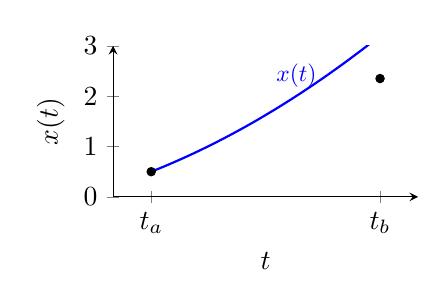
\begin{tikzpicture}
\begin{axis}[
  width=0.45\textwidth, height=3.5cm,
  xlabel={$t$}, ylabel={$x(t)$},
  xmin=0, xmax=4, ymin=0, ymax=3,
  xtick={0.5,3.5}, xticklabels={$t_a$,$t_b$},
  ytick={}, axis lines=left,
]
  \addplot[thick,blue,domain=0.5:3.5,samples=60]
    {0.5+0.6*(x-0.5)+0.1*(x-0.5)^2} node[pos=0.6,above,scale=0.85]{$x(t)$};
  \addplot[only marks,mark=*,mark size=1.5pt] coordinates {(0.5,0.5)(3.5,2.35)};
\end{axis}
\end{tikzpicture}
\end{center}
\caption{The path $x(t)$ of a 1-D particle between fixed endpoints at times $t_a$ and $t_b$. The Lagrangian $L(x,\dot{x},t)$ characterises how each path is weighted by the action $S = \int_{t_a}^{t_b} L\,dt$.}
\label{fig:1d_path}
\end{figure}

\begin{itemize}
    \item Assume there is some function $L(x, \dot{x}, t)$ that in some way
        characterises the path.
    \item We can't find $L$ with a finite number of points (infinite number of paths
        go through any finite set of points).
\end{itemize}

Therefore we must look at the \textbf{action}:
\[
    S = \int_{t_a}^{t_b} L(x, \dot{x}, t)\,dt + C
    + \underbrace{\int_{t_a}^{t_b} \dv{t}\!\left[f(x,t)\right]dt}_{\text{total time derivative — set to 0}}.
\]

$S$ is a \textbf{functional}: a function of a function $x(t)$.

\begin{itemize}
    \item \textbf{Assertion 1:} Any additive constant $C$ can be set to 0 (analogous
        to the constant in a potential).
    \item \textbf{Assertion 2:} The red (total-derivative) term is also constant if it
        is the integral of a derivative of some function of time (e.g.\ $2t^2$).
\end{itemize}

\subsection{Examining the Postulates}

\begin{itemize}
    \item \textbf{Postulate 1:} $\dot{x} \to \dot{x} + V$ (Galilean transformation).
        In both frames the physics is the same $\Rightarrow \delta S = 0$ (up to a
        constant) $\Rightarrow$ path can't change meaningfully.
    \item \textbf{Postulate 2:}
        \begin{itemize}
            \item $t + \delta t \Rightarrow \delta S = 0$ (equations of motion must be
                time-translation invariant).
            \item $x + \delta x \Rightarrow \delta S = 0$ (space-translation invariance).
            \item $x \to -x$ $(\dot{x} \to -\dot{x}) \Rightarrow \delta S = 0$
                (rotation invariance).
        \end{itemize}
\end{itemize}

\subsection{Determining the Free Lagrangian}

Define $L_\mathrm{Free}^{1\text{-D}} \equiv K(x, \dot{x}, t)$.

\begin{itemize}
    \item $K$ cannot have pure terms that are functions of $t$ alone (from Assertion 2).
    \item $x \to -x \Rightarrow \delta S = 0 \Rightarrow K(-x, -\dot{x}, t) = K(x, \dot{x}, t)$.
    \item Try a polynomial: $K = C_0 + C_2 x^2 + C_4 x^4 + C_{-2}x^{-2} + \cdots$
    \item $x \to x + \delta x \Rightarrow \delta S = 0 \Rightarrow x^2 \to (x+\delta x)^2
        = x^2 + \underbrace{\delta x^2}_{\text{const. so far}} + \underbrace{2\delta x\, x}_{\text{not const.}}$
        \textbf{Problem!}
    \item \textbf{No pure functions of $x$ work!}
\end{itemize}

Try $K = C_2 \dot{x}^2 + C_4 \dot{x}^4 + \cdots$:
\begin{align*}
    (\dot{x} + V)^2 &= \dot{x}^2 + V^2 + 2\dot{x}V = \dot{x}^2 + \dv{t}[2Vx] \checkmark \\
    (\dot{x} + V)^4 &= \dot{x}^4 + V^4 + 4\dot{x}^3 V + 6V^2\dot{x}^2 + 4V\dot{x}^3 \;\times
        \quad \text{(cannot be written as a total derivative)}
\end{align*}

\begin{itemize}
    \item The only function that works is $K(\dot{x}) = C\dot{x}^2$.
    \item Because the only intrinsic property of a point particle is its mass,
        \[
            K(\dot{x}) = \alpha(m)\,m\dot{x}^2.
        \]
    \item Assume $K(\dot{x})$ has units of $[E]$, so $\alpha(m)$ is dimensionless.
\end{itemize}

\begin{figure}[H]
    \centering
    \caption{The action $S$ as a functional of the path. The minimum (orange dot)
    corresponds to the physical path. When $\dot{x} \to \dot{x}+V$, $S$ translates
    up and down, so neither absolute values of $S$ nor $\Delta S$ matter (different
    units).}
\end{figure}

$S$ has units of $[\text{J}][\text{s}]$.

\begin{itemize}
    \item Different inertial frames should agree on extremum points.
    \item Paths that are similar are close; paths that are different are far apart.
\end{itemize}

% -----------------------------------------------------------------------
\section{Extremising the Action: Euler–Lagrange Equation}

We want
\[
    S[x_0(t) + \delta(t)] - S[x_0(t)] = 0.
\]

Notice $\delta(t_a) = \delta(t_b) = 0$.

Take a Taylor expansion of $\delta S$:
\[
    \delta S = 0 = \int_{t_a}^{t_b}
    \left[\frac{\partial L}{\partial x}(x - x_0)
    + \frac{\partial L}{\partial \dot{x}}(\dot{x} - \dot{x}_0)\right]dt.
\]

Note that
\[
    \dv{t}\!\left[\frac{\partial L}{\partial \dot{x}}\,\delta\right]
    = \frac{\partial L}{\partial \dot{x}}\,\dot{\delta}
    + \left[\dv{t}\frac{\partial L}{\partial \dot{x}}\right]\delta.
\]

Replacing the $\frac{\partial L}{\partial \dot{x}}\dot{\delta}$ term:
\[
    \Rightarrow \int_{t_a}^{t_b} dt\,\delta\!\left[
        \frac{\partial L}{\partial x} - \dv{t}\frac{\partial L}{\partial \dot{x}}
    \right]
    + \left[\frac{\partial L}{\partial \dot{x}}\,\delta\right]_{t_a}^{t_b} = 0.
\]

The boundary term vanishes because $\delta(t_a) = \delta(t_b) = 0$.

\begin{formula}[Euler--Lagrange Equation]
    \[
        \boxed{\frac{\partial L}{\partial x} - \dv{t}\frac{\partial L}{\partial \dot{x}} = 0}
    \]
\end{formula}

Substituting $L = \alpha(m)\,m\dot{x}^2$:
\[
    \frac{\partial L}{\partial x} - \dv{t}\frac{\partial L}{\partial \dot{x}}
    = 0 - \dv{t}\!\left[2\alpha(m)\,m\dot{x}\right] = 0
    \;\Rightarrow\; \dot{x} = \text{const.}
\]

This is Newton's First Law for a free particle.

% -----------------------------------------------------------------------
\section{Two-Particle System}

\begin{figure}[H]
    \centering
    \caption{Two particles on a line, with positions $x_1$, $x_2$, velocities
    $\dot{x}_1$, $\dot{x}_2$, and masses $m_1$, $m_2$.}
\end{figure}

Now
\[
    S = \int_{t_a}^{t_b} L(x_1, \dot{x}_1, x_2, \dot{x}_2, t)\,dt.
\]

Once again assume $\delta_i(t_a) = \delta_i(t_b) = 0$ for $i = 1, 2$.  Then
\[
    \delta S = 0 \Rightarrow
    \int_{t_a}^{t_b} dt \left[
        \frac{\partial L}{\partial x_1}(x_1 - x_1^0)
        + \frac{\partial L}{\partial \dot{x}_1}(\dot{x}_1 - \dot{x}_1^0)
        + \frac{\partial L}{\partial x_2}(x_2 - x_2^0)
        + \frac{\partial L}{\partial \dot{x}_2}(\dot{x}_2 - \dot{x}_2^0)
    \right] = 0.
\]

You can set $\delta_1 = 0$ to examine $\delta_2$, and vice versa, because they must
work for all $\delta_1, \delta_2$.  Therefore
\[
    L_\mathrm{Free}^{1\text{-D}}
    = K(\dot{x}_1) + K(\dot{x}_2)
    = \alpha(m_1)\,m_1\dot{x}_1^2 + \alpha(m_2)\,m_2\dot{x}_2^2.
\]

% -----------------------------------------------------------------------
\chapter{Calculus of Variations}

\textit{(Recitation 1: Review of Calculus of Variations, Monday January 6, 2025)}

\section{Total vs.\ Partial Derivatives}

Suppose $f(t, x(t), y(t)) : \mathbb{R} \to \mathbb{R}$.

\subsection{Partial Derivative $\partial f / \partial t$}

Assume all variables fixed, except $t$.

\begin{example}[Partial Derivative]
    \[
        f(t, x, y) = t^3 + 2x + 3ty
        \;\Rightarrow\;
        \frac{\partial f}{\partial t} = 3t^2 + 0 + 3y.
    \]
\end{example}

In general, for $f(\vec{x}(t))$ where $\vec{x}(t) = (x_1(t), x_2(t), \ldots, x_n(t))$:

\begin{formula}[Total Derivative]
    \[
        \dv{f}{t} = \sum_{i=1}^{N} \frac{\partial f}{\partial x_i}\dv{x_i}{t}.
    \]
\end{formula}

For $f(t, x(t), y(t))$ where $x, y$ are also functions of $t$:
\[
    \dv{f}{t}
    = \frac{\partial f}{\partial t}\cdot\frac{\partial t}{\partial t}
    + \frac{\partial f}{\partial x}\frac{\partial x}{\partial t}
    + \frac{\partial f}{\partial y}\frac{\partial y}{\partial t}.
\]

\begin{example}[Total Derivative]
    \[
        \dv{f}{t} = 3t^2 + 3y + 2\dot{x} + 3t\dot{y}.
    \]
\end{example}

\subsection{Local and Convective Derivative}

For $f(t) = f(t, x(t), y(t), z(t))$:
\[
    \dv{f}{t}
    = \frac{\partial f}{\partial t}
    + \frac{\partial f}{\partial x}\frac{\partial x}{\partial t}
    + \frac{\partial f}{\partial y}\frac{\partial y}{\partial t}
    + \frac{\partial f}{\partial z}\frac{\partial z}{\partial t}.
\]

The velocity vector is $\vec{v} = (\dot{x}, \dot{y}, \dot{z})$ and the gradient is
$\nabla f = \frac{\partial f}{\partial x}\hat{x} + \frac{\partial f}{\partial y}\hat{y}
+ \frac{\partial f}{\partial z}\hat{z}$.  Thus
\[
    \dv{f}{t}
    = \underbrace{\frac{\partial f}{\partial t}}_{\text{local derivative}}
    + \underbrace{\vec{v}\cdot\nabla f}_{\text{convective derivative}}.
\]

% -----------------------------------------------------------------------
\section{Calculus of Variations}

The action $S[f(t,\vec{q})]$ is a \textbf{functional}: input a function, output a
scalar, where $S : (f[\mathbb{R}, \mathbb{R}]) \to \mathbb{R}$.

\begin{example}[General Functional]
    \[
        J[y_i] = \int_{x_1}^{x_2} dx\; F\!\left(y_1(x), \ldots, y_N(x),\,
        y_1'(x), \ldots, y_N'(x),\, x\right).
    \]
    $y_i(x)$ can be maximised, minimised, or set to 0.
\end{example}

\textbf{Calculus of Variations (CoV):} Want a set of functions that extremise the
functional, i.e.\ $\delta J = 0$.

\begin{itemize}
    \item Use small variations to find maxima/minima of our functional $J$.
    \item Consider $y_i^* = y_i(x) + \delta y_i(x)$ where
        $|\delta y_i(x)| \ll |y_i(x)|$, $|\delta y_i'| \ll y_i'(x)$.
    \item Constraint: $\delta y(x_1) = \delta y(x_2) = 0$,
        $\delta y'(x_1) = \delta y'(x_2) = 0$.
\end{itemize}

\begin{figure}[H]
    \centering
    \caption{The extremal path $y_i(x)$ and a neighbouring varied path $y_i^*$ between
    fixed endpoints $x_1$ and $x_2$.}
\end{figure}

\subsection{Computing the Variation}

\[
    \delta J = J[y + \delta y] - J[y]
    = \int_{x_1}^{x_2} F\!\left[y+\delta y,\;\frac{dy}{dx}+\delta\frac{du}{dx},\;x\right]dx
    - \int_{x_1}^{x_2} F\!\left[y,\;\frac{dy}{dx},\;x\right]dx.
\]

Write the first integrand as a Taylor series.

\subsubsection{Taylor Series}

\[
    F(x, y) \approx F(x_0, y_0)
    + (x - x_0)\left.\frac{\partial F}{\partial x}\right|_{\substack{x=x_0\\y=y_0}}
    + (y - y_0)\left.\frac{\partial F}{\partial y}\right|_{\substack{x=x_0\\y=y_0}}
    + O(\delta^2).
\]

Let $y_0 = y$, $y_0' = y'$, so
\[
    F(y+\delta y,\; y'+\delta y',\; x)
    \approx F(y, y', x) + (\delta y)\frac{\partial F}{\partial y}
    + \delta y'\frac{\partial F}{\partial y'} + O(\delta^2).
\]

Therefore
\begin{align*}
    \delta J
    &= \int_{x_1}^{x_2} dx\left[F(y,y',x) + \frac{\partial F}{\partial y}\delta y
       + \frac{\partial F}{\partial y'}\delta y'\right]
     - \int_{x_1}^{x_2} dx\left[F(y,y',x)\right] \\
    &= \int_{x_1}^{x_2} dx\left[\frac{\partial F}{\partial y}\delta y
       + \frac{\partial F}{\partial y'}\delta y'\right].
\end{align*}

Integrate the second term by parts ($\int u\,dv = uv - \int v\,du$):
\[
    \int_{x_1}^{x_2} dx\left(\frac{\partial F}{\partial y'}\right)\delta y'
    = \left.\frac{\partial F}{\partial y'}\delta y\right|_{x_1}^{x_2}
    - \int_{x_1}^{x_2} \delta y \cdot \dv{x}\!\left(\frac{\partial F}{\partial y'}\right)dx.
\]

(Here $u = \partial F/\partial y'$ and $dv = \delta y'\,dx$.)

\[
    \Rightarrow\;
    \delta J = \int_{x_1}^{x_2} dx\left[
        \frac{\partial F}{\partial y} - \dv{x}\!\left(\frac{\partial F}{\partial y'}\right)
    \right]\delta y \;\neq 0.
\]

\[
    \Rightarrow\; \delta J = 0
    \;\Rightarrow\;
    \frac{\partial L}{\partial q} - \dv{t}\!\left(\dv{L}{\dot{q}}\right) = 0
\]

with the substitution $F \to L$, $J \to S$, $x \to t$.

% -----------------------------------------------------------------------
\chapter{Particle Interactions and Example Usage}

\textit{(Lecture: Particle Interactions and Example Usage, Tuesday January 7, 2025)}

\section{From Last Time}

\[
    L_\mathrm{Free}^{1\text{-D}}
    = \alpha(m_1)\,m_1\dot{x}_1^2 + \alpha(m_2)\,m_2\dot{x}_2^2,
    \quad \text{has dimensions of } E.
\]

% -----------------------------------------------------------------------
\section{Conservative Interactions}

\begin{itemize}
    \item Work done by a force is path-independent.
    \item $\vec{F} = -\nabla\phi$ — force is the negative gradient of a potential.
\end{itemize}

\[
    L = L_\mathrm{Free}^{1\text{-D}} + \mathcal{I}(x_1, x_2).
\]

Applying the postulates again:
\begin{itemize}
    \item $x_i \to x_i + \delta x_i \Rightarrow \delta S = 0$:
        this means $\mathcal{I}$ must depend on $x_1 - x_2$ (invariant to translation).
    \item $x_i \to -x_i \Rightarrow \delta S = 0$:
        this means $\mathcal{I}$ depends on $|x_1 - x_2|$ (depends on distance).
\end{itemize}

Let $\Delta x \equiv |x_1 - x_2|$.
\[
    L = \alpha(m_1)\,m_1\dot{x}_1^2 + \alpha(m_2)\,m_2\dot{x}_2^2
    + \underbrace{\beta\, U(\Delta x)}_{\text{potential function}}.
\]

Plugging into Euler--Lagrange for $x_1$:
\[
    \frac{\partial L}{\partial x_1} - \dv{t}\frac{\partial L}{\partial \dot{x}_1}
    = 0
    = \beta\frac{\partial U}{\partial \Delta x}\frac{\partial \Delta x}{\partial x_1}
    - \dv{t}\!\left[2\alpha(m_1)\,m_1\dot{x}_1\right].
\]
\[
    \Rightarrow\; 2\alpha(m_1)\,m_1\ddot{x}_1 = \pm\beta\frac{\partial U}{\partial \Delta x}
    = -\beta F(\Delta x).
\]

By convention $2\alpha(m_1) = 1$, $\beta = -1$:
\[
    \boxed{m_1\ddot{x}_1 = F(\Delta x)} \quad \textbf{Newton's Second Law}.
\]

Doing the same for $x_2$: $m_2\ddot{x}_2 = -F(\Delta x)$ (the absolute value
derivative has the opposite sign) — \textbf{Newton's Third Law}.

% -----------------------------------------------------------------------
\section{Example: Using the Lagrangian}

A mass $m$ on a spring with spring constant $k$ (no friction, displacement $x$):
\[
    L = K \ominus U = \tfrac{1}{2}m\dot{x}^2 - \tfrac{1}{2}kx^2.
\]

(The minus sign comes from quantum mechanics / the potential convention.)

Applying Euler--Lagrange:
\[
    \frac{\partial L}{\partial x} - \dv{t}\frac{\partial L}{\partial \dot{x}} = 0
    \;\Rightarrow\;
    -kx - \dv{t}\!\left[m\dot{x}\right] = 0
    \;\Rightarrow\; m\ddot{x} = -kx.
\]

% -----------------------------------------------------------------------
\section{Lagrangian in 3 Dimensions}

\[
    L = K(\dot{\vec{x}}_1) + K(\dot{\vec{x}}_2) - U(|\vec{x}_1 - \vec{x}_2|).
\]

\begin{itemize}
    \item Now $L$ needs to be rotationally invariant.
    \item $\Rightarrow K = \tfrac{1}{2}m\,\dot{\vec{x}}\cdot\dot{\vec{x}}
        = \tfrac{1}{2}m(\dot{x}^2 + \dot{y}^2 + \dot{z}^2)$.
    \item There are just 3 Euler--Lagrange equations, one for each coordinate.
\end{itemize}

% -----------------------------------------------------------------------
\section{Example 2: Sphere Rolling on a Sliding Wedge}

\begin{figure}[H]
    \centering
    \caption{A sphere of mass $m_s$ and radius $R$ rolls without slipping on a
    frictionless wedge of mass $m_w$ and angle $\alpha$ that slides freely on a
    frictionless surface. $x$ is the position of the wedge; $\theta$ is the rotation
    angle of the sphere.}
\end{figure}

Neither friction (at the wedge--floor interface) nor slip (at the sphere--wedge
interface): $L = K - U$.

Coordinates:
\[
    \vec{x}_w = x\hat{x}, \qquad
    \vec{x}_s = (x + R\theta\cos\alpha)\hat{x} - R\theta\sin\alpha\,\hat{y}.
\]

Kinetic energies:
\begin{align*}
    K &= \tfrac{1}{2}m_w\dot{x}^2
       + \tfrac{1}{2}m_s\left[(\dot{x} + R\dot{\theta}\cos\alpha)^2
         + (R\dot{\theta}\sin\alpha)^2\right]
       + \tfrac{1}{2}\cdot\tfrac{2}{5}m_s R^2\dot{\theta}^2, \\
    U &= -m_s g R\theta\sin\alpha.
\end{align*}

\[
    L = \tfrac{1}{2}m_w\dot{x}^2
      + \tfrac{1}{2}m_s\!\left[\dot{x}^2 + R^2\dot{\theta}^2
        + 2R\dot{x}\dot{\theta}\cos\alpha\right]
      + \tfrac{1}{5}m_s R^2\dot{\theta}^2 + m_s g R\theta\sin\alpha.
\]

\subsection{Applying Euler--Lagrange}

\textit{For $x$:}
\[
    \frac{\partial L}{\partial x} - \dv{t}\frac{\partial L}{\partial \dot{x}}
    = 0 = 0 - \dv{t}\!\left[m_w\dot{x} + m_s\dot{x} + m_s R\dot{\theta}\cos\alpha\right].
\]
\[
    \Rightarrow\; (m_w + m_s)\ddot{x} + m_s R\ddot{\theta}\cos\alpha = 0. \tag{1}
\]
\[
    \Rightarrow\; \ddot{x} = \frac{-m_s R\cos\alpha}{m_w + m_s}\,\ddot{\theta}.
\]

\textit{For $\theta$:}
\[
    \frac{\partial L}{\partial \theta} - \dv{t}\frac{\partial L}{\partial \dot{\theta}}
    = 0
    = m_s g R\sin\alpha
    - \dv{t}\!\left[m_s R^2\dot{\theta} + m_s R\dot{x}\cos\alpha
        + \tfrac{2}{5}m_s R^2\dot{\theta}\right].
\]
\[
    \Rightarrow\; \tfrac{7}{5}R\ddot{\theta} + \ddot{x}\cos\alpha = g\sin\alpha. \tag{2}
\]

Combining (1) and (2):
\[
    R\ddot{\theta}\left[\frac{7}{5} - \frac{m_s R\cos^2\alpha}{m_w+m_s}\right]
    = g\sin\alpha.
\]

Defining $\beta \equiv \frac{7}{5} - \frac{m_s R\cos^2\alpha}{m_w+m_s}$:
\[
    \boxed{\ddot{\theta} = \frac{g\sin\alpha}{\beta R}}
    \;\Rightarrow\;
    \theta(t) = \frac{1}{2}\frac{g\sin\alpha}{\beta R}\,t^2,
    \qquad
    \boxed{x(t) = \frac{-m_s R\cos\alpha}{m_w+m_s}\,\theta(t).}
\]

% -----------------------------------------------------------------------
\section{Motivation for the Action (Quantum Mechanics)}

\begin{itemize}
    \item The assumption of classical mechanics is that a particle takes a definite
        path from $a$ to $b$.
    \item In quantum mechanics,
        \[
            \mathrm{prob}(a \to b)
            \propto \left|\int_\text{paths} e^{i S_\text{path}/\hbar}\right|^2.
        \]
        (The argument must be dimensionless — hence $\hbar$.)
    \item ``Crazy'' paths cancel out.
    \item Ones near the ``main path'' add up.
\end{itemize}

\begin{figure}[H]
    \centering
    \caption{In the path integral picture, contributions from paths far from the
    stationary-phase path cancel due to rapid oscillation of the phase, while
    nearby paths interfere constructively.}
\end{figure}

% -----------------------------------------------------------------------
\chapter{More Euler--Lagrange Examples}

\textit{(Recitation 2: More Euler--Lagrange Examples, Tuesday January 7, 2025)}

\section{Recap}

Define the functional $J[y_i]$:
\[
    J[y_i] = \int_{x_1}^{x_2} dx\; F(y, y', x).
\]

In order for $y(x)$ to extremise $J$ ($\delta J = 0$):
\[
    \frac{\partial F}{\partial y} - \dv{x}\!\left(\frac{\partial F}{\partial y'}\right) = 0.
\]

With $F \to L = T - U$, $x \to t$, $y \to q$:
\[
    \frac{\partial L}{\partial q} - \dv{t}\!\left(\frac{\partial L}{\partial \dot{q}}\right) = 0.
\]

\begin{formula}[Hamilton's Principle]
    The motion of a system $q(t)$ between $t_1$ and $t_2$ is a stationary
    point/extremum of the action functional
    \[
        S[q(t)] = \int_{t_1}^{t_2} L\!\left(q(t), \dot{q}(t), t\right)dt.
    \]
    The Euler--Lagrange equations yield the dynamics.
\end{formula}

% -----------------------------------------------------------------------
\section{Example: Straight Line in Euclidean Space}

We want to find the shortest distance between two points in a flat plane.

\begin{figure}[H]
    \centering
    \caption{Two points $A$ and $B$ in the $xy$-plane connected by a curve $y(x)$
    between $x=a$ and $x=b$.  The length element is $d\ell$.}
\end{figure}

\[
    d\ell^2 = dx^2 + dy^2
    \;\Rightarrow\;
    d\ell = \sqrt{dx^2 + dy^2} = dx\sqrt{1 + \left(\dv{y}{x}\right)^2}.
\]

\[
    \Rightarrow\; \ell[y] = \int_a^b dx\left(1 + \left(\dv{y}{x}\right)^2\right)^{1/2}.
\]

We showed that any functional $J = \int_{x_1}^{x_2} F(y, y', x)\,dx$ is extremised
when
\[
    \frac{\partial F}{\partial y_i} - \dv{x}\!\left(\frac{\partial F}{\partial y_i'}\right) = 0.
\]

With $F = (1 + y'(x))^{1/2}$, $J \to \ell$:
\[
    \frac{\partial F}{\partial y} = 0, \qquad
    -\dv{x}\!\left(\frac{\partial F}{\partial y'}\right)
    = -\dv{x}\!\left(\tfrac{1}{2}(1 + y'(x)^2)^{-1/2}\cdot 2y'(x)\right)
    = -\dv{x}\!\left(\frac{y'}{(1+y'(x)^2)^{1/2}}\right) = 0.
\]

\[
    \Rightarrow\; \frac{y'(x)}{(1 + y'(x)^2)^{1/2}} = C
    \;\Rightarrow\; y'(x) = C(1 + y'(x)^2)^{1/2}.
\]
\[
    y'^2(x) = C^2(1 + y'(x)^2)
    \;\Rightarrow\; y'^2(x)(1 - C^2) = C^2
    \;\Rightarrow\; y'(x) = K \text{ (constant)}.
\]
\[
    \boxed{y(x) = Kx + C.}
\]

% -----------------------------------------------------------------------
\section{Example: Masses on a String}

\begin{figure}[H]
    \centering
    \caption{Mass $m_1$ hangs vertically through a hole in a frictionless table
    attached to a string of length $\ell$. Mass $m_2 = m$ is on the table and moves
    in polar coordinates $(r,\theta)$. Gravity acts in $-\hat{z}$. No friction on
    the table.}
\end{figure}

Setup:
\begin{itemize}
    \item String length $\ell$; no friction on table; gravity in $-\hat{z}$.
    \item $m_1 = m_2 = m$.
    \item $m_1$ only moves up and down (length below table $= \ell - r$).
\end{itemize}

Want: equations of motion for both masses.  Use $L = T - U$.

\textit{Kinetic energies:}
\[
    T_1 = \tfrac{1}{2}m_1 v_1^2 = \tfrac{1}{2}m\left(\dv{t}(\ell - r)\right)^2
        = \tfrac{1}{2}m\dot{r}^2.
\]
\[
    T_2 = \tfrac{1}{2}mv_2^2 = \tfrac{1}{2}m_2(v_r^2 + v_\theta^2)
        = \tfrac{1}{2}m(\dot{r}^2 + r^2\dot{\theta}^2).
\]

\textit{Potential energies:}
\[
    U_2 = 0 \text{ (by choice)}, \qquad U_1 = mg(-(\ell - r)).
\]

\[
    \Rightarrow\; L_1 = T_1 + T_2 - U_1 - U_2
    = \tfrac{1}{2}m\dot{r}^2 + \tfrac{1}{2}m(\dot{r}^2 + r^2\dot{\theta}^2) + mg(\ell - r).
\]

($mg\ell$ is usually dropped as it is a constant.)

\subsection{Applying Euler--Lagrange}

\textit{For $r$:}
\[
    \frac{\partial L}{\partial r} = mr\dot{\theta}^2 - mg, \qquad
    \frac{\partial L}{\partial \dot{r}} = 2m\dot{r}
    \;\Rightarrow\; \dv{t}(\cdots) = 2m\ddot{r}.
\]
\[
    \therefore\; 2m\ddot{r} = mr\dot{\theta}^2 - mg
    \;\Rightarrow\; \boxed{\ddot{r} = \tfrac{r}{2}\dot{\theta}^2 - \tfrac{g}{2}.}
\]

\textit{For $\theta$:}
\[
    \frac{\partial L}{\partial \theta} = 0, \qquad
    \frac{\partial L}{\partial \dot{\theta}} = mr^2\dot{\theta}
    \;\Rightarrow\;
    \dv{t}(\cdot\cdot) = (mr^2\ddot{\theta} + m\dot{\theta}\cdot 2r\dot{r}) = 0.
\]
\[
    \boxed{\ddot{\theta} = -\frac{2}{r}\dot{r}\dot{\theta}.}
\]

% -----------------------------------------------------------------------
\chapter{Symmetry and Noether's Theorem}

\textit{(Lecture: Symmetry and Noether's Theorem, Wednesday January 8, 2025)}

\section{Time Derivative of the Lagrangian}

\[
    \dv{L}{t}
    = \frac{\partial L}{\partial t}
    + \sum_i\left[\frac{\partial L}{\partial q_i}\dv{q_i}{t}
        + \frac{\partial L}{\partial \dot{q}_i}\dv{\dot{q}_i}{t}\right].
\]

By Euler--Lagrange, $\frac{\partial L}{\partial q_i} = \dv{t}\frac{\partial L}{\partial \dot{q}_i}$,
which simplifies the above to
\[
    = \frac{\partial L}{\partial t}
    + \sum_i\left[\left(\dv{t}\frac{\partial L}{\partial \dot{q}_i}\right)\dot{q}_i
        + \frac{\partial L}{\partial \dot{q}_i}\ddot{q}_i\right]
    = \frac{\partial L}{\partial t}
    + \sum_i \dv{t}\!\left[\frac{\partial L}{\partial \dot{q}_i}\dot{q}_i\right].
\]

Therefore,
\[
    \dv{t}\!\left[\sum_i \frac{\partial L}{\partial \dot{q}_i}\dot{q}_i - L\right]
    = -\frac{\partial L}{\partial t}.
\]

\begin{itemize}
    \item Time translation is a symmetry of the system.
    \item For an isolated system, $\frac{\partial L}{\partial t} = 0$ (the Lagrangian
        cannot be an explicit function of time; implicit functions such as $\dot{x}$
        don't count).
\end{itemize}

\begin{formula}[Conservation of Energy]
    \[
        \boxed{\sum_i \frac{\partial L}{\partial \dot{q}_i}\dot{q}_i - L
        \;\text{ is conserved.}}
    \]
\end{formula}

\begin{example}[Energy from the Lagrangian]
    For $L = \tfrac{1}{2}m_1\dot{x}_1^2 + \tfrac{1}{2}m_2\dot{x}_2^2 - U(|x_1-x_2|)$:
    \begin{align*}
        \frac{\partial L}{\partial \dot{x}_1}\dot{x}_1
        + \frac{\partial L}{\partial \dot{x}_2}\dot{x}_2 - L
        &= m_1\dot{x}_1\dot{x}_1 + m_2\dot{x}_2\dot{x}_2
         - \tfrac{1}{2}m_1\dot{x}_1^2 - \tfrac{1}{2}m_2\dot{x}_2^2 + U \\
        &= K + U = E.
    \end{align*}
\end{example}

Energy conservation is a result of the postulates!  It holds when there is no
explicit time dependence in the Lagrangian.

% -----------------------------------------------------------------------
\section{Conservation of Momentum (Space-Translation Invariance)}

Recall space-translation invariance: $x_1 \to x_1 + \delta x$.  This is a
first-order Taylor expansion of the change in the Lagrangian:
\[
    \delta L = 0 = \sum_i \frac{\partial L}{\partial x_i}\delta x.
\]

By Euler--Lagrange, $\frac{\partial L}{\partial x_i} = \dv{t}\frac{\partial L}{\partial \dot{x}_i}$:
\[
    \sum_i\left[\dv{t}\frac{\partial L}{\partial \dot{x}_i}\right]\delta x = 0
    \;\Rightarrow\;
    \dv{t}\!\left[\sum_i \frac{\partial L}{\partial \dot{x}_i}\right] = 0.
\]

\begin{formula}[Conservation of Momentum]
    \[
        \boxed{\sum_i \frac{\partial L}{\partial \dot{x}_i} \;\text{ is conserved!}}
    \]
\end{formula}

\begin{example}
    \[
        \frac{\partial L}{\partial \dot{x}_1} + \frac{\partial L}{\partial \dot{x}_2}
        = m_1\dot{x}_1 + m_2\dot{x}_2 = p_1^x + p_2^x \equiv p_x.
    \]
    Momentum is conserved in every direction when space translation is a symmetry.
\end{example}

Symmetries in a system lead to conserved quantities!

% -----------------------------------------------------------------------
\section{Conservation of Angular Momentum (Rotation Invariance)}

Now use the fact that space-time is isotropic.  Consider a rotation $\delta\phi$
about $\hat{z}$:
\begin{align*}
    x_i &\to x_i\cos\delta\phi - y_i\sin\delta\phi
          \approx x_i - y_i\delta\phi
          \;\Rightarrow\; \delta x_i = -y_i\delta\phi, \\
    y_i &\to y_i\cos\delta\phi + x_i\sin\delta\phi
          \approx y_i + x_i\delta\phi
          \;\Rightarrow\; \delta y_i = x_i\delta\phi, \\
    z_i &\to z_i
          \;\Rightarrow\; \delta z_i = 0.
\end{align*}

\[
    \delta L = 0 = \sum_i\left[
        \frac{\partial L}{\partial x_i}\delta x_i
        + \frac{\partial L}{\partial \dot{x}_i}\delta\dot{x}_i
        + \frac{\partial L}{\partial y_i}\delta y_i
        + \frac{\partial L}{\partial \dot{y}_i}\delta\dot{y}_i
    \right].
\]

Applying Euler--Lagrange and using the chain rule trick
\[
    \dv{t}\!\left[\frac{\partial L}{\partial \dot{x}_i}y_i\right]
    = \left(\dv{t}\frac{\partial L}{\partial \dot{x}_i}\right)y_i
    + \frac{\partial L}{\partial \dot{x}_i}\dot{y}_i,
\]
the sum becomes
\[
    = \dv{t}\!\left[\sum_i\!\left(\frac{\partial L}{\partial \dot{x}_i}(-y_i)
    + \frac{\partial L}{\partial \dot{y}_i}x_i\right)\right] = 0.
\]

\begin{formula}[Conservation of Angular Momentum ($z$-direction)]
    \[
        \boxed{\frac{\partial L}{\partial \dot{x}_i}(-y_i)
        + \frac{\partial L}{\partial \dot{y}_i}x_i \;\text{ is conserved!}}
        \quad \text{Angular Momentum ($z$-direction).}
    \]
\end{formula}

\begin{example}
    For $L = \sum_i \tfrac{1}{2}m_i(\dot{x}_i^2 + \dot{y}_i^2 + \dot{z}_i^2) - U$:
    \[
        \sum_i(-m\dot{x}_i y_i + m\dot{y}_i x_i)
        = \sum_i(\dot{\vec{x}}\times\vec{p}_i)_z
        = \sum_i \ell_z^i \equiv \ell_z.
    \]
    This is the $z$-component of angular momentum of the system.
\end{example}

\begin{theorem}[Noether's Theorem]
    Every symmetry leads to a conserved quantity such as energy, momentum,
    or angular momentum.  To ask if some quantity is conserved, just check if
    it is a symmetry of the Lagrangian.
\end{theorem}

% -----------------------------------------------------------------------
\section{Reduced Action}

Recall
\[
    S = \int L\,dt = \int (K - U)\,dt \quad \text{(for a conservative system).}
\]

Restrict to only paths that have the same energy: use $E = K + U$.

\[
    \Rightarrow\; S_0 = \int (2K - \underbrace{E}_{\text{constant}})\,dt
    = \int m\dot{\vec{x}}\cdot\dot{\vec{x}}\,dt
    = \int \vec{p}\cdot\dv{\vec{x}}{t}\,dt
    = \int_{\vec{x}_a}^{\vec{x}_b} \vec{p}\cdot d\vec{x}.
\]

\begin{formula}[Reduced Action]
    \[
        S_0 = \int_{\vec{x}_a}^{\vec{x}_b} \vec{p}\cdot d\vec{x}.
    \]
\end{formula}

\begin{itemize}
    \item If $U = \text{const} \Rightarrow$ no force $\Rightarrow$ momentum is
        constant.  Thus $S_0 = p\,\ell_{ab}$ (path length).
    \item Path has to be a flat (straight) line.
\end{itemize}

When does this work?
\begin{itemize}
    \item We assume the information about $a$ and $b$ completely determines the
        problem.
    \item Another assumption: the particle could only take one path.  (Violated when
        the system is ``open''.)  Violated by dissipative systems in general, but
        sometimes they do work.
\end{itemize}

\begin{example}[Lagrangian for a Damped Oscillator]
    \[
        L = e^{\gamma t}\!\left(\frac{m}{2}(\dot{x}^2 - \omega^2 x^2)\right).
    \]
    \[
        \frac{\partial L}{\partial x} - \dv{t}\frac{\partial L}{\partial \dot{x}}
        = -e^{\gamma t} m\omega^2 x - \dv{t}\!\left[e^{\gamma t}m\dot{x}\right]
        = e^{\gamma t}\omega^2 x + e^{\gamma t}\ddot{x} + \dot{x}\gamma e^{\gamma t} = 0.
    \]
    \[
        \Rightarrow\; \ddot{x} + \gamma\dot{x} + \omega^2 x = 0.
    \]
    Another way: $L = e^{\gamma t}\!\left(\tfrac{1}{2}m\dot{x} - U(x)\right)$
    $\Rightarrow m\ddot{x} = -\frac{\partial U}{\partial x} - m\gamma\dot{x}$.
\end{example}

If you have non-conservative dissipative effects that you don't know how to put
into the Lagrangian:
\[
    \dv{t}\frac{\partial L}{\partial \dot{x}} - \frac{\partial L}{\partial x}
    = \sum_i F_i^x
    \quad \text{(only works if the conservative Lagrangian doesn't depend on the
    dissipative forces)}.
\]

% -----------------------------------------------------------------------
\chapter{Non-Inertial Reference Frames}

\textit{(Lecture: Non-Inertial Reference Frames, Thursday January 9, 2025)}

\section{Easiest Case: Linearly Accelerating Frame}

\begin{figure}[H]
    \centering
    \caption{A particle at coordinates $(x, y)$ in a frame that accelerates with
    velocity $V(t)$ to the right.}
\end{figure}

The frame is accelerating (velocity non-constant).

Write $T$ as it would be seen from some inertial frame in the coordinates of the
non-inertial frame, in addition to the motion of the non-inertial frame:
\[
    L = \tfrac{1}{2}m\left|\dot{\vec{x}} + \vec{V}(t)\right|^2 - U.
\]

Here $\dot{\vec{x}}$ is the velocity in the non-inertial frame and $\vec{V}(t)$ is a
total time derivative so $= 0$ in the E-L sense.

Expanding:
\[
    L = \tfrac{1}{2}m|\dot{\vec{x}}|^2 + m\dot{\vec{x}}\cdot\vec{V} + \tfrac{1}{2}m|\vec{V}|^2 - U.
\]

Applying Euler--Lagrange for $x_1$:
\[
    \frac{\partial L}{\partial x} - \dv{t}\frac{\partial L}{\partial \dot{x}}
    = 0 = -\frac{\partial U}{\partial x} - \dv{t}\!\left[m\dot{x} + mV(t)\right].
\]
\[
    \Rightarrow\; m\ddot{x} = -\frac{\partial U}{\partial x} - m\dot{V}(t).
\]

The extra term $-m\dot{V}(t)$ is the \textbf{fictitious force} in the accelerating frame.

% -----------------------------------------------------------------------
\section{Hardest Case: Rotating Frame}

\begin{figure}[H]
    \centering
    \caption{A frame rotating at rate $\Omega$ about the $z$-axis. A particle has
    position $(r,\theta)$ in the rotating frame.}
\end{figure}

Frame rotating at rate $\Omega$; $\vec{\Omega} = \Omega\hat{z}$.

In the inertial frame:
\[
    \vec{v} = \dot{r}\rhat + r\dot{\theta}\tthat, \qquad
    \vec{a} = (\ddot{r} - r\dot{\theta}^2)\rhat
            + (r\ddot{\theta} + 2\dot{r}\dot{\theta})\tthat, \qquad
    \vec{\nabla} = \frac{\partial}{\partial r}\rhat + \frac{1}{r}\frac{\partial}{\partial\theta}\tthat.
\]

\subsection{8.01 Approach}

\begin{align*}
    \vec{F}_\text{Coriolis}   &= -2m\vec{\Omega}\times\vec{v}
        = -2m\Omega[\dot{r}\tthat - r\dot{\theta}\rhat], \\
    \vec{F}_\text{centrifugal} &= -m\vec{\Omega}\times(\vec{\Omega}\times\vec{r})
        = m\Omega^2 r\,\rhat.
\end{align*}

$\hat{r}$ component of Newton's second law:
\[
    m(\ddot{r} - r\dot{\theta}^2) = -\frac{\partial U}{\partial r} + m\Omega^2 r + 2m\Omega r\dot{\theta}.
\]

$\hat{\theta}$ component:
\[
    m(r\ddot{\theta} + 2\dot{r}\dot{\theta}) = -\frac{1}{r}\frac{\partial U}{\partial\theta} - 2m\Omega\dot{r}.
\]

\subsection{Lagrangian Approach}

All we do is add $\Omega$ to the angular velocity:
\[
    L = \tfrac{1}{2}m|\vec{v}|^2 - U
    = \tfrac{1}{2}m\!\left(\dot{r}^2 + r^2(\dot{\theta}+\Omega)^2\right) - U.
\]

\textit{$\hat{r}$ component:}
\begin{align*}
    \frac{\partial L}{\partial r} - \dv{t}\frac{\partial L}{\partial \dot{r}}
    &= mr(\dot{\theta}+\Omega)^2 - \frac{\partial U}{\partial r} - \dv{t}[m\dot{r}] \\
    &= mr\left[\dot{\theta}^2 + 2\dot{\theta}\Omega + \Omega^2\right]
       - \frac{\partial U}{\partial r} - m\ddot{r} = 0.
\end{align*}
\[
    \boxed{m\ddot{r} - mr\dot{\theta}^2 = 2mr\Omega\dot{\theta} - \frac{\partial U}{\partial r} + m\Omega^2 r.}
    \tag{1}
\]

\textit{$\hat{\theta}$ component:}
\begin{align*}
    \frac{\partial L}{\partial \theta} - \dv{t}\frac{\partial L}{\partial \dot{\theta}}
    &= -\frac{\partial U}{\partial \theta} - \dv{t}\!\left[mr^2(\dot{\theta}+\Omega)\right] \\
    &= -\frac{\partial U}{\partial \theta} - m2r\dot{r}(\dot{\theta}+\Omega) - mr^2\ddot{\theta}.
\end{align*}
\[
    \boxed{m(r^2\ddot{\theta} + 2r\dot{r}\dot{\theta}) = -\frac{\partial U}{\partial\theta} - 2mr\dot{r}\Omega.}
    \quad \text{Torque equation (just divide by }r\text{).} \tag{2}
\]

% -----------------------------------------------------------------------
\section{Example: Lagrange Points}

\begin{figure}[H]
    \centering
    \caption{The Earth--Sun system rotating at $\Omega$. The Sun has mass $M_\odot$,
    the Earth has mass $m_e$, total mass $M = m_e + M_\odot$. The Earth--Sun
    distance is $R$. A test mass $m$ is placed at position $(r,\theta)$ in the
    rotating frame.}
\end{figure}

\begin{itemize}
    \item Assume Earth's orbit is elliptical.
    \item Let $M = m_e + M_\odot$; Earth--Sun distance $= R$.
    \item Kepler's Law: $\Omega^2 = \frac{GM}{R^3}$.
    \item Let $M_{\odot,e} \gg m$.
\end{itemize}

Is there anywhere we can put $m$ where it doesn't move in the frame of the
Earth/Sun? (Lagrange point.)  We want $\dot{r} = \ddot{r} = \dot{\theta} = \ddot{\theta} = 0$.

\textit{Plugging into the Lagrangian equations of motion:}

(2): $m(0 + 0) = -\frac{\partial U}{\partial\theta} = 0$ ($\theta$ direction).

(1): $\frac{\partial U}{\partial r} = mr\Omega^2$.

The potential is
\[
    U = -\frac{GM_\odot m}{r_\odot} - \frac{Gm_e m}{r_e}.
\]

\textit{Doing approximations,} with $r_{\odot,e}$ the distance from $m$ to the Sun/Earth:
\[
    r_{\odot,e}^2
    = \left(r\cos\theta \pm R\frac{m_{e/\odot}}{M}\right)^2 + r^2\sin^2\theta
    = r^2 \pm 2rR\cos\theta\frac{m_{e/\odot}}{M} + R^2\frac{m_{e/\odot}^2}{M^2} + \cdots
\]

From $\frac{\partial U}{\partial\theta} = 0$:
\[
    \frac{\partial U}{\partial\theta}
    = \frac{\partial U}{\partial r_\odot}\frac{\partial r_\odot}{\partial\theta}
    + \frac{\partial U}{\partial r_e}\frac{\partial r_e}{\partial\theta} = 0.
\]

With $2r_{\odot,e}\frac{\partial r_{\odot,e}}{\partial\theta} = \mp 2R\frac{m_{e/\odot}}{M}r\sin\theta$:
\[
    \frac{\partial U}{\partial\theta}
    = -Gm\left[\frac{m_\odot}{r_\odot^2}\!\left(\frac{-Rm_e r\sin\theta}{r_\odot M}\right)
    - \frac{m_e}{r_e^2}\!\left(\frac{Rm_\odot r m\sin\theta}{r_e M}\right)\right] = 0.
\]
\[
    \Rightarrow\; \frac{r\sin\theta}{r_\odot^3} = \frac{r\sin\theta}{r_e^3}
    \;\Rightarrow\; r\sin\theta \neq 0
    \;\Rightarrow\; r_e = r_\odot.
\]

\textit{Next step} (radial equation, $r$ direction):
\[
    mr\Omega^2 = \frac{\partial U}{\partial r}
    = \frac{\partial U}{\partial r_\odot}\frac{\partial r_\odot}{\partial r}
    + \frac{\partial U}{\partial r_e}\frac{\partial r_e}{\partial r}.
\]

Expanding:
\[
    = Gm\left[\frac{m_\odot}{r_\odot^3}\!\left(r + R\frac{m_e}{M}\cos\theta\right)
    + \frac{m_e}{r_e^3}\!\left(r - R\frac{m_\odot}{M}\cos\theta\right)\right]
    = mr\frac{GM}{r^3}.
\]

Looking for solutions with $r_e = r_\odot$:
\[
    = \frac{1}{r_\odot^3}\left[m_\odot r + 0 + m_e r\right]
    \;\Rightarrow\; \frac{rM}{r_\odot^3} = \frac{rM}{R^3}.
\]

This gives $r_\odot = R$, so the Lagrange points are at the vertices of an
equilateral triangle.

% -----------------------------------------------------------------------
\chapter{Double Pendulum}

\textit{(Recitation 4: Double Pendulum, Thursday January 9, 2025)}

\section{Example: Double Pendulum}

\begin{figure}[H]
    \centering
    \caption{Double pendulum: mass $m_1$ suspended on a rod of length $\ell_1$
    at angle $\theta_1$; mass $m_2$ suspended from $m_1$ on a rod of length
    $\ell_2$ at angle $\theta_2$.  $x = 0$ is the pivot.}
\end{figure}

$U = 0 - \cdots$  (choose reference).

Find $L$; use $L$ to find equations of motion.  Best to start with Cartesian
coordinates.

\textit{Coordinates:}
\begin{align*}
    x_1 &= \ell_1\sin(\theta_1), & x_2 &= \ell_1\sin(\theta_1) + \ell_2\sin(\theta_2), \\
    y_1 &= -\ell_1\cos(\theta_1), & y_2 &= -\ell_1\cos(\theta_1) - \ell_2\cos(\theta_2).
\end{align*}

\textit{Velocities:}
\begin{align*}
    \dot{x}_1 &= \ell_1\cos(\theta_1)\dot{\theta}_1, &
    \dot{x}_2 &= \ell_1\cos\theta_1\dot{\theta}_1 + \ell_2\cos\theta_2\dot{\theta}_2, \\
    \dot{y}_1 &= \ell_1\sin(\theta_1)\dot{\theta}_1, &
    \dot{y}_2 &= \ell_1\sin\theta_1\dot{\theta}_1 + \ell_2\sin\theta_2\dot{\theta}_2.
\end{align*}

\textit{Kinetic energies:}
\[
    T_1 = \tfrac{1}{2}m_1(\ell_1^2\dot{\theta}_1^2).
\]

\[
    T_2 = \tfrac{1}{2}m_2(\dot{x}_2^2 + \dot{y}_2^2)
\]
\begin{align*}
    &= \tfrac{1}{2}m_2\Bigl[
        \ell_1^2\cos^2\theta_1\dot{\theta}_1^2 + \ell_2^2\cos^2\theta_2\dot{\theta}_2^2
        + 2\ell_1\ell_2\cos\theta_1\cos\theta_2\dot{\theta}_1\dot{\theta}_2 \\
    &\qquad + \ell_1^2\sin^2\theta_1\dot{\theta}_1^2 + \ell_2^2\sin^2\theta_2\dot{\theta}_2^2
        + 2\ell_1\ell_2\sin\theta_1\sin\theta_2\dot{\theta}_1\dot{\theta}_2
    \Bigr] \\
    &= \tfrac{1}{2}m_2\!\left(\ell_1^2\dot{\theta}_1^2 + \ell_2^2\dot{\theta}_2^2
        + 2\ell_1\ell_2\dot{\theta}_1\dot{\theta}_2\cos(\theta_1 - \theta_2)\right).
\end{align*}

\textit{Potential energies:}
\[
    U_1 = -m_1 g\ell_1\cos\theta_1, \qquad
    U_2 = -m_2 g(\ell_1\cos\theta_1 + \ell_2\cos\theta_2).
\]

\textit{Full Lagrangian:}
\begin{align*}
    L &= \tfrac{1}{2}m_1\!\left(\ell_1^2\dot{\theta}_1^2\right)
       + \tfrac{1}{2}m_2\!\left(\ell_1^2\dot{\theta}_1^2 + \ell_2^2\dot{\theta}_2^2
         + 2\ell_1\ell_2\dot{\theta}_1\dot{\theta}_2\cos(\theta_1-\theta_2)\right) \\
      &\quad - m_1 g\ell_1\cos\theta_1 - m_2 g(\ell_1\cos\theta_1 + \ell_2\cos\theta_2).
\end{align*}

\begin{itemize}
    \item Next step: apply Euler--Lagrange equations for $\theta_1$ and $\theta_2$.
\end{itemize}

% Lec. 5: Normal Modes — Friday, January 10, 2025

\chapter{Normal Modes, Gravity, and the Virial Theorem}

\section{Normal Coordinates}

\[
    x_i = \sum_j C_{ij} q_j \qquad \text{(linear combination of coordinates)}
\]

For linear systems,
\[
    \Rightarrow\quad \alpha_i \ddot{x}_i + \beta_i \dot{x}_i + \gamma x_i = f_i(t)
\]

\subsection{Example: Mechanical Vibrations in Molecules}

\begin{figure}[H]
\begin{center}
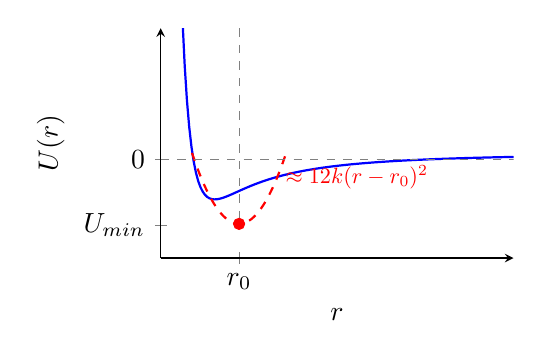
\begin{tikzpicture}
\begin{axis}[
  width=0.5\textwidth, height=4.5cm,
  xlabel={$r$}, ylabel={$U(r)$},
  xmin=0.5, xmax=5, ymin=-1.5, ymax=2.0,
  xtick={1.5}, xticklabels={$r_0$},
  ytick={0,-1.0}, yticklabels={$0$,$U_\text{min}$},
  axis lines=left, samples=150,
]
  % Lennard-Jones like potential
  \addplot[thick,blue,domain=0.72:5]{(1/(x^6)) - (1.5/x^2) + 0.1};
  % Minimum marker
  \addplot[only marks,mark=*,mark size=2pt,red] coordinates {(1.5,-0.98)};
  \draw[dashed,gray] (axis cs:1.5,2.0) -- (axis cs:1.5,-0.98);
  % Harmonic approximation (parabola near minimum)
  \addplot[thick,dashed,red,domain=0.9:2.1]{-0.98 + 3.0*(x-1.5)^2}
    node[pos=0.85,right,scale=0.8]{$\approx \tfrac{1}{2}k(r-r_0)^2$};
  % Zero level
  \addplot[dashed,gray,domain=0.5:5]{0};
\end{axis}
\end{tikzpicture}
\end{center}
\caption{Interatomic potential $U(r)$ vs.\ separation $r$, showing a minimum at equilibrium distance $r_0$. Near the minimum, $U$ is well approximated by a parabola (harmonic approximation, red dashed).}
\label{fig:interatomic_pot}
\end{figure}

\begin{itemize}
    \item Potential is about $r_0$ constant (i.e.\ $\approx 0$ to first order).
    \item Taylor expand about equilibrium $r_0$:
    \[
        U(r - r_0) \approx U(r_0) + \left.\frac{\partial U}{\partial r}\right|_{r=r_0}(r - r_0)
        + \frac{1}{2}\left.\frac{\partial^2 U}{\partial r^2}\right|_{r=r_0}(r-r_0)^2 + \cdots
    \]
    The first-order term vanishes at equilibrium; the second-order coefficient is $> 0$ because it is a stable equilibrium.
\end{itemize}

Thus for \underline{any} system that is near a stable equilibrium point,

\begin{formula}[Harmonic approximation near equilibrium]
\[
    U(r) \approx \tfrac{1}{2}k(r - r_0)^2
\]
\end{formula}

\subsection{Example: CO\textsubscript{2} molecule ($\text{C} = \text{O} = \text{C}$)}

\begin{figure}[H]
\begin{center}
\begin{tikzpicture}[scale=1.0, >=Stealth]
  % Wall anchors (none needed — free molecule)
  % Atom O (left)
  \fill[red!70] (0,0) circle[radius=0.25];
  \node[below] at (0,-0.3) {O};
  \node[above,scale=0.8] at (0,0.3) {$m_O$};
  % Displacement x1 arrow
  \draw[->,blue,thin] (0,-0.55) -- (0.4,-0.55) node[right,scale=0.8]{$x_1$};
  % Spring 1
  \draw[thick, decorate, decoration={zigzag,segment length=5pt,amplitude=3pt}]
    (0.25,0) -- (1.75,0);
  \node[above,scale=0.8] at (1.0,0.2) {$k$};
  % Atom C (centre)
  \fill[gray!70] (2.0,0) circle[radius=0.2];
  \node[below] at (2.0,-0.3) {C};
  \node[above,scale=0.8] at (2.0,0.3) {$m_C$};
  % Displacement x2 arrow
  \draw[->,blue,thin] (2.0,-0.55) -- (2.4,-0.55) node[right,scale=0.8]{$x_2$};
  % Spring 2
  \draw[thick, decorate, decoration={zigzag,segment length=5pt,amplitude=3pt}]
    (2.2,0) -- (3.75,0);
  \node[above,scale=0.8] at (3.0,0.2) {$k$};
  % Atom O (right)
  \fill[red!70] (4.0,0) circle[radius=0.25];
  \node[below] at (4.0,-0.3) {O};
  \node[above,scale=0.8] at (4.0,0.3) {$m_O$};
  % Displacement x3 arrow
  \draw[->,blue,thin] (4.0,-0.55) -- (4.4,-0.55) node[right,scale=0.8]{$x_3$};
\end{tikzpicture}
\end{center}
\caption{CO$_2$ modelled as three masses connected by two springs of spring constant $k$: O--spring--C--spring--O. Displacements $x_1$, $x_2$, $x_3$ are measured from equilibrium positions.}
\label{fig:co2_springs}
\end{figure}

\begin{itemize}
    \item Treat atoms as point particles.
    \item Total DOF: $3 \times 3 = 9$ normal modes \quad (3 atoms $\times$ 3 spatial coords).
    \item But there will be 3 trivial translation modes $\Rightarrow 9 - 3 = 6$.
    \item Also there are 2 rotation modes $\Rightarrow 6 - 2 = 4$ normal modes for vibrations.
\end{itemize}

The Lagrangian (considering only 1D motion along the axis, with oxygen masses $m_O$ and carbon mass $m_C$):
\[
    L = \tfrac{1}{2}m_O(\dot{x}_1^2 + \dot{x}_3^2) + \tfrac{1}{2}m_C(m_C \dot{x}_2^2)
        - \tfrac{1}{2}k(x_2 - x_1)^2 - \tfrac{1}{2}k(x_3 - x_2)^2
\]

Applying the Euler--Lagrange equation for $x_1$:
\[
    \frac{\partial L}{\partial x_1} - \frac{d}{dt}\frac{\partial L}{\partial \dot{x}_1} = 0
    = -k(x_1 - x_2) - \frac{d}{dt}(m_O \dot{x}_1)
    \quad\Rightarrow\quad
    \ddot{x}_1 + \frac{k}{m_O}(x_1 - x_2) = 0 \tag{1}
\]

By $x_1 \leftrightarrow x_3$ symmetry:
\[
    \ddot{x}_3 + \frac{k}{m_O}(x_3 - x_2) = 0 \tag{3}
\]

For $x_2$:
\[
    \frac{\partial L}{\partial x_2} - \frac{d}{dt}\frac{\partial L}{\partial \dot{x}_2} = 0
    \quad\Rightarrow\quad
    \ddot{x}_2 + \frac{k}{m_C}(2x_2 - x_2 - x_3) \tag{2}
\]

\textbf{Ansatz:} Try $x_i = C_i e^{i\omega t}$.

Plugging into (1):
\[
    -\omega^2 C_1 e^{i\omega t} + \frac{k}{m_O}(C_1 - C_2)e^{i\omega t} = 0
\]
\[
    (2): \quad -\omega^2 C_2 e^{i\omega t} + \frac{k}{m_C}(2C_2 - C_1 - C_3)e^{i\omega t} = 0
\]
\[
    (3): \quad -\omega^2 C_3 e^{i\omega t} + \frac{k}{m_O}(C_3 - C_2)e^{i\omega t} = 0
\]

Writing in matrix form:
\[
    \begin{pmatrix}
        \dfrac{k}{m_O} - \omega^2 & -\dfrac{k}{m_O} & 0 \\[8pt]
        -\dfrac{k}{m_C} & \dfrac{2k}{m_C} - \omega^2 & -\dfrac{k}{m_C} \\[8pt]
        0 & -\dfrac{k}{m_O} & \dfrac{k}{m_O} - \omega^2
    \end{pmatrix}
    \begin{pmatrix} C_1 \\ C_2 \\ C_3 \end{pmatrix}
    =
    \begin{pmatrix} 0 \\ 0 \\ 0 \end{pmatrix}
\]

Set $\det A = 0$:
\[
    \left(\frac{k}{m_O} - \omega^2\right)
    \left[\left(\frac{2k}{m_C} - \omega^2\right)\left(\frac{k}{m_O} - \omega^2\right)
    - \frac{k^2}{m_O m_C}\right]
    + \frac{k}{m_O}\cdot\frac{-k}{m_C}\left(\frac{k}{m_O} - \omega^2\right) = 0
\]
\[
    \omega^2\left(\frac{k}{m_O} - \omega^2\right)\left(\omega^2 - \frac{2k}{m_C} - \frac{k}{m_O}\right) = 0
\]

\textbf{Solutions:}

\begin{itemize}
    \item $\omega^2 = 0 \Rightarrow C_1 = C_2 = C_3$ $\Rightarrow$ linear translation.
    \[
        \begin{pmatrix}0\\0\\0\end{pmatrix} \quad \lambda = 7\,\mu\text{m}
    \]

    \item $\omega_a^2 = \dfrac{k}{m_O} \Rightarrow C_2 = 0,\; C_1 = -C_3 \Rightarrow x_1(t) = -x_3(t)$.
    \[
        \begin{pmatrix}1\\0\\-1\end{pmatrix} \quad \lambda_a = \text{DNE (no dipole, because no displacement of C)}
    \]

    \item $\omega_b^2 = \left(\dfrac{2k}{m_C} + \dfrac{k}{m_O}\right)
    \Rightarrow C_2 = -\dfrac{2m_O}{m_C}C_1,\; C_1 = C_3$.
    \[
        x_1(t) = x_3(t), \quad x_2(t) = -\frac{2m_O}{m_C}x_1(t)
        \quad\Rightarrow\quad
        \begin{pmatrix}1 \\ -\frac{2m_O}{m_C} \\ 1\end{pmatrix}e^{i\omega t}
        \quad \lambda_b = 4\,\mu\text{m}
    \]
\end{itemize}

\begin{example}[Application: QM absorption lines]
In QM, $\lambda = \dfrac{2\pi c}{\omega}$. We know $k \sim 140\,\text{eV}$.
Based on whether a dipole moment forms, we can calculate absorption lines of molecules.
\end{example}

\subsection{2D Molecule Modes}

Look for modes where the center of mass doesn't move.

\begin{figure}[H]
\centering
\caption{A bent triatomic molecule with two outer atoms (mass $m_O$) displaced transversely by $y$, and the central atom (mass $m_C$) displaced by $y_2$ vertically. The bonds make an angle with the horizontal.}
\end{figure}

COM condition:
\[
    m_O(-y - y) + m_C y_2 = 0 \quad\Rightarrow\quad y_2 = \frac{2m_O}{m_C}y
\]

The Lagrangian (with $k_\perp$ the transverse spring constant, noting there is only one oscillation so no double-counting):
\begin{align*}
    L &= 2 \cdot \tfrac{1}{2}m_O \dot{y}^2 + \tfrac{1}{2}m_C\left(\frac{2m_O}{m_C}\dot{y}\right)^2
    - \tfrac{1}{2}k_\perp\left[2\left(y + \frac{2m_O}{m_C}y\right)\right]^2 \\
    &= \dot{y}^2\left(m_O + \frac{2m_O^2}{m_C}\right) - 2k_\perp\left(1 + \frac{2m_O}{m_C}\right)^2 y^2
\end{align*}

Applying the Euler--Lagrange equation:
\[
    \frac{\partial L}{\partial y} - \frac{d}{dt}\frac{\partial L}{\partial \dot{y}}
    = -4k_\perp y\left(1 + \frac{2m_O}{m_C}\right)^2 - \frac{d}{dt}\left[2\dot{y}\,m_O\!\left(1 + \frac{2m_O}{m_C}\right)\right]
\]
\[
    \Rightarrow\quad \ddot{y} + 2k_\perp\left(\frac{1}{m_O} + \frac{2}{m_C}\right)y = 0
\]
\[
    \Rightarrow\quad \omega_\perp^2 = 2k_\perp\left(\frac{1}{m_O} + \frac{2}{m_C}\right)
\]

% -------------------------------------------------------
% Lec. 6: Gravity — Monday, January 13, 2025
% -------------------------------------------------------

\chapter{Gravity and Orbital Mechanics}

\section{Kepler's Laws (Empirical)}

\begin{enumerate}
    \item The orbit of every planet is an ellipse with the Sun at one of the two foci.
    \item A line joining a planet to the Sun sweeps out equal area in equal time.
    \item $T^2 \sim (\text{semi-major axis length})^3$.
\end{enumerate}

\begin{itemize}
    \item Any time you have a point source that radiates uniformly, the density goes like $r^{-2}$ (because surface area is $4\pi r^2$).
    \item Gravity can be thought of like radiation.
\end{itemize}

\section{Newton's Argument}

Near the surface of the Earth:
\[
    mg = \frac{G M_E m}{r^2} \quad \text{($G M_E$ unknown)}
\]

For the Moon in circular orbit:
\[
    m_m \frac{v_m^2}{D_{e\text{-}m}} = \frac{G M_E m_m}{D_{e\text{-}m}^2}, \qquad v_m = \frac{2\pi D_{e\text{-}m}}{T_m}
\]
\[
    \Rightarrow\quad \frac{4\pi^2 D_{e\text{-}m}}{T_m^2} = \frac{G M_E}{D_{e\text{-}m}} = \frac{g R_E^2}{D_{e\text{-}m}}
\]
\[
    \Rightarrow\quad
    \boxed{T_m \stackrel{?}{=} \frac{2\pi D_{e\text{-}m}^{3/2}}{R_E \sqrt{g}}}
\]
This is testable because $g$, $R_E$, $T_m$ are known; you can use parallax to measure distance to the Moon.

\begin{example}[Eratosthenes]
Precise measurement of the radius of the Earth.
\[
    R_E = \frac{D}{\theta}
\]
\begin{figure}[H]
\centering
\caption{Two observers separated by distance $D$ on the Earth's surface measure the Sun at different angles; the central angle $\theta$ gives $R_E = D/\theta$.}
\end{figure}
\end{example}

\section{Two-Body Orbital Problem}

\begin{figure}[H]
\centering
\caption{Two masses $m_1$ and $m_2$ in the COM frame, with separation $r$ and angle $\theta$. Distances from COM: $\frac{m_2}{M}r$ for $m_1$ and $\frac{m_1}{M}r$ for $m_2$.}
\end{figure}

\begin{itemize}
    \item Consider the COM frame: $\sum p_i = 0$ (conserved momentum).
    \item Distances from COM are as follows (with $M = m_1 + m_2$):
    \[
        r_1 = \frac{m_2}{M}r, \qquad r_2 = \frac{m_1}{M}r
    \]
    \item Motion must be confined to a plane (in this case the board) --- no out-of-plane motion.
\end{itemize}

\begin{align*}
    L &= \tfrac{1}{2}m_1\left[\left(\frac{m_2}{M}\dot{r}\right)^2 + \left(\frac{m_2}{M}r\dot\theta\right)^2\right]
       + \tfrac{1}{2}m_2\left[\left(\frac{m_1}{M}\dot{r}\right)^2 + \left(\frac{m_1}{M}r\dot\theta\right)^2\right]
       + \frac{Gm_1 m_2}{r} \\
    &= \frac{m_1 m_2}{2M^2}\left[\dot{r}^2(m_2 + m_1) + r^2\dot\theta^2(m_2 + m_1)\right] + \frac{Gm_1 m_2}{r}
\end{align*}

Define the \emph{reduced mass}:
\begin{formula}[Reduced mass]
\[
    \frac{1}{\mu} = \frac{1}{m_1} + \frac{1}{m_2} = \frac{M}{m_1 m_2}
    \quad\Rightarrow\quad \mu = \frac{m_1 m_2}{M}
\]
\end{formula}

\[
    \Rightarrow\quad L = \tfrac{1}{2}\mu(\dot{r}^2 + r^2\dot\theta^2) + \frac{Gm_1 m_2}{r}
\]

This is equivalent to a single particle of mass $\mu$ at distance $r$ from the origin in a gravitational field.

\subsection{Conservation of Angular Momentum}

\[
    \frac{\partial L}{\partial \theta} - \frac{d}{dt}\frac{\partial L}{\partial \dot\theta}
    = 0 - \frac{d}{dt}(\mu r^2 \dot\theta) = 0
\]
Angular momentum is conserved:
\[
    \ell \equiv \mu r^2 \dot\theta = \text{const}
    \quad\Rightarrow\quad \dot\theta = \frac{\ell}{\mu r^2}
\]

In general, if $\dfrac{\partial L}{\partial \dot{q}} = \dfrac{\partial L}{\partial q} = 0$, then $\dfrac{\partial L}{\partial \dot{q}}$ is conserved.

\section{Finding Kepler's Laws}

\subsection{Kepler's Second Law}

\begin{figure}[H]
\centering
\caption{In a small time $\delta t$, the radius sweeps out a triangle of area $\delta A \approx \frac{1}{2}r^2\,\delta\theta$.}
\end{figure}

\[
    \delta A \approx \tfrac{1}{2}(r + \delta r)\,r\,d\theta \approx \tfrac{1}{2}r^2\,\delta\theta
\]
\[
    \delta t \to 0 \quad\Rightarrow\quad \frac{dA}{dt} = \tfrac{1}{2}r^2\dot\theta = \frac{\ell}{2\mu} = \text{const} \quad\checkmark
\]

\subsection{Lagrangian Equation for $r$}

\[
    \frac{\partial L}{\partial r} - \frac{d}{dt}\left(\frac{\partial L}{\partial \dot r}\right) = 0
    \quad\Rightarrow\quad
    \mu r\dot\theta^2 - \frac{Gm_1 m_2}{r^2} - \frac{d}{dt}\left[\mu\dot{r}\right] = 0
\]
\[
    \mu\ddot{r} = \frac{\ell^2}{\mu r^3} - \frac{Gm_1 m_2}{r^2} \quad \text{(quite challenging to solve directly)}
\]

Note that $\dfrac{\partial L}{\partial t} = 0 \Rightarrow$ Energy is conserved:
\[
    E = \frac{\partial L}{\partial \dot{r}}\dot{r} + \frac{\partial L}{\partial \dot\theta}\dot\theta - L
    = \mu\dot{r}\dot{r} + \mu r^2\dot\theta\dot\theta - L
\]
\[
    \Rightarrow\quad E = \tfrac{1}{2}\mu\dot{r}^2 + \tfrac{1}{2}\mu r^2\dot\theta^2 - \frac{Gm_1 m_2}{r}
    = \tfrac{1}{2}\mu\dot{r}^2 + \underbrace{\frac{\ell^2}{2\mu r^2} - \frac{Gm_1 m_2}{r}}_{U_\text{eff}(r)}
\]

The first term comes out of kinetic energy; the bracketed part defines $U_\text{eff}(r)$.

\[
    \dot{r} = \pm\sqrt{\frac{2}{\mu}\bigl(E - U_\text{eff}(r)\bigr)}
\]

To solve for the \emph{shape} of the orbit (not time evolution):
\[
    d\theta = \frac{d\theta}{dt}\frac{dt}{dr}dr = \frac{\dot\theta}{\dot{r}}dr
    = \frac{\ell}{\mu r^2 \dot{r}}dr
\]
\[
    \int_0^{2\pi}d\theta = \int \frac{\ell}{\mu r^2}
    \left(\sqrt{\frac{2}{\mu}\bigl(E - U_\text{eff}(r)\bigr)}\right)^{-1} dr
\]

\section{Proving Kepler's 3rd Law}

Assume (these are properties of an ellipse):
\[
    a = \frac{\alpha}{1 - \varepsilon^2}, \qquad b = \sqrt{\alpha a}
\]
where $a$ is the semi-major axis.

\begin{figure}[H]
\centering
\caption{Ellipse with semi-major axis $a$ and semi-minor axis $b$.}
\end{figure}

Also assume:
\[
    A_\text{ellipse} = \pi ab = \pi\sqrt{\alpha}\,a^{3/2} = \pi\frac{\ell}{\mu\sqrt{GM}}\,a^{3/2}
\]

But we also know that $A_\text{ellipse} = \displaystyle\int_0^T \frac{dA}{dt}\,dt = \frac{\ell}{2\mu}T$.

\[
    \Rightarrow\quad \frac{\ell}{2\mu}T = \pi\frac{\ell}{\mu\sqrt{GM}}\,a^{3/2}
\]

\begin{formula}[Kepler's 3rd Law]
\[
    \boxed{T^2 = \frac{4\pi^2 a^3}{GM}}
\]
\end{formula}

\begin{example}[Finding mass of a star]
Since $M \propto \dfrac{a^3}{T^2}$,
\[
    \frac{M}{M_\odot} \propto
    \left[\frac{a_\text{S-z}}{a_{e\text{-}m}}\right]^3
    \left[\frac{T_{e\text{-}m}}{T_\text{S-z}}\right]^2
    \approx \left[\frac{1000\,\text{AU}}{1}\right]^3\!\left[\frac{1\,\text{yr}}{16\,\text{yr}}\right]^2
    \approx \frac{10^9}{256}
\]
\[
    \Rightarrow\quad M \approx 4 \times 10^6\,M_\odot
\]
\end{example}

% -------------------------------------------------------
% Rec. 6: COM Frame Example — Monday, January 13, 2025
% -------------------------------------------------------

\section{Springs in a Plane (Recitation: COM Frame Example)}

\begin{figure}[H]
\centering
\caption{Two masses $m_1$ (at $(x_1,y_1)$) and $m_2$ (at $(x_2,y_2)$) connected by a spring with spring constant $k$ and unstretched length $b$. The system can rotate and oscillate.}
\end{figure}

\begin{itemize}
    \item Spring constant $k$, unstretched length $b$, the system can rotate and oscillate.
    \item $L = T - U$
    \item $T_i = \tfrac{1}{2}m_i(\dot x_i^2 + \dot y_i^2)$
    \item $U_s = \tfrac{1}{2}k\!\left(\sqrt{(x_2-x_1)^2+(y_2-y_1)^2} - b\right)^2$ --- a mess to differentiate.
\end{itemize}

Move to the COM frame with coordinates $(R_{\text{cm},x},\, R_{\text{cm},y},\, r,\, \theta)$:
\[
    \mu = \frac{m_1 m_2}{m_1 + m_2}, \qquad M = m_1 + m_2
\]

In these coordinates, the Lagrangian is:
\[
    L = \underbrace{\tfrac{1}{2}M\dot{R}_\text{cm}^2}_{\text{KE of COM}}
      = \underbrace{\tfrac{1}{2}M(\dot R_x^2 + \dot R_y^2)}_{\text{KE of COM}}
      + \underbrace{\tfrac{1}{2}\mu(\dot{r}^2 + r^2\dot\theta^2)}_{\text{motion of }\mu}
      - \underbrace{\tfrac{1}{2}k(r-b)^2}_{\text{spring}}
\]

Equations of motion:
\begin{itemize}
    \item $R_\text{cm}$: $\dfrac{\partial L}{\partial R_\text{cm}} = 0 \Rightarrow R_\text{cm}$ is ignorable $\Rightarrow \dfrac{\partial L}{\partial \dot R_\text{cm}} = M\dot R_\text{cm} = P_\text{cm}$ is conserved (linear momentum).

    \item $\theta$: $\dfrac{\partial L}{\partial \theta_\text{cm}} = 0 \Rightarrow \theta_\text{cm}$ is ignorable $\Rightarrow \dfrac{\partial L}{\partial \dot\theta_\text{cm}} = \mu r^2\dot\theta \equiv P_\theta$ is conserved (angular momentum of $\mu$).
    \[
        \Rightarrow\quad \dot\theta = \frac{P_\theta}{\mu r^2}
    \]

    \item $r$:
    \[
        \frac{d}{dt}\left(\frac{\partial L}{\partial \dot r}\right) - \frac{\partial L}{\partial r}
        = \mu\ddot{r} - \mu r\dot\theta^2 + k(r-b) = 0
        = \mu\ddot{r} - \frac{\mu P_\theta^2}{\mu r^3} + k(r-b) = 0
    \]
\end{itemize}

Central potentials can be described with effective potentials:
\[
    U_\text{eff} = U_S(r) + f(r, P_\theta)
\]

We want $\mu\ddot{r} = -\dfrac{\partial U_\text{eff}}{\partial r}$, so take the antiderivative of $\dfrac{P_\theta^2}{\mu r^3}$:
\[
    U_\text{eff}(r) = \frac{k(r-b)^2}{2} + \frac{P_\theta^2}{2\mu r^2}
\]

\begin{figure}[H]
\centering
\caption{Effective potential $U_\text{eff}(r)$ showing the centrifugal barrier for $P_\theta > 0$ (curve shifted up) versus $P_\theta = 0$. Minimum occurs at $r = b$ for $P_\theta = 0$.}
\end{figure}

\textbf{Rotating but not oscillating} ($\dot\theta \neq 0$, $\dot r = \ddot r = 0$):

Since $\mu\ddot{r} = -\dfrac{dU_\text{eff}}{dr}$, requiring $\dot r = \ddot r = 0$ means $\dfrac{dU_\text{eff}}{dr} = 0$.

We also know that since angular momentum is conserved, $\dfrac{d}{dt}(\mu r^2 \dot\theta) = 0 \Rightarrow \dot\theta$ constant.
\[
    \Rightarrow\quad k(r-b) = \mu r\dot\theta^2
    \quad \text{intuition: ``spring force'' = ``centripetal force''}
\]

\textbf{Oscillating but not rotating} ($\ddot r \neq 0$, $\dot\theta = \ddot\theta = 0$):
\[
    \text{EOM:}\quad \mu\ddot{r} = -k(r-b)
\]
Rewrite as $\Delta\ddot{r} = -\dfrac{k}{\mu}\Delta r$ where $\Delta r \equiv r - b$.

Energy:
\[
    E = T(\dot{r}) + U_\text{eff}(r, P_\theta), \qquad \frac{\partial L}{\partial t} = 0 \Rightarrow E\text{ conserved}
\]

% -------------------------------------------------------
% Lec. 7: Gravity Cont. — Tuesday, January 14, 2025
% -------------------------------------------------------

\section{Gravity Continued: Orbit Shape and General Central Potentials}

\subsection{Recap: Orbit Equation}

\begin{figure}[H]
\centering
\caption{Two-body system reduced to a single particle of mass $\mu$ at separation $r$, angle $\theta$, in an effective gravitational potential.}
\end{figure}

The orbit solution is:
\[
    r(\theta) = \frac{\alpha}{1 + \varepsilon\cos\theta}
\]
\begin{figure}[H]
\centering
\caption{Ellipse showing peri- (closest approach) and apo- (farthest point) of the orbit.}
\end{figure}

\begin{itemize}
    \item In the limit $m_1 \ll m_2$: $m_2$ sits at the origin and $m_1$ traces out the ellipse.
    \item If $m_1 = m_2$, both objects orbit the COM, each tracing an ellipse around it.
\end{itemize}

\subsection{Energy and Orbit Classification}

\[
    E = \tfrac{1}{2}\mu\dot{r}^2 + \frac{\ell^2}{2\mu r^2} + U(r), \qquad
    \mu = \frac{m_1 m_2}{M}, \quad U_\text{eff}(r),\quad U(r) = -\frac{Gm_1 m_2}{r}
\]

\begin{figure}[H]
\centering
\caption{Effective potential $U_\text{eff}(r) = \frac{\ell^2}{2\mu r^2} - \frac{Gm_1 m_2}{r}$ showing three energy levels $E_0 < E_1 < 0 < E_2$. $E_0$: circular orbit; $E_1$: ellipse; $E \geq 0$: hyperbola (parabola for $E=0$).}
\end{figure}

\begin{itemize}
    \item For $E_1$ (negative, above minimum): the trajectory is an ellipse.
    \item For $E_0$ (at minimum): the trajectory is circular. Most objects fall into circular orbit.
    \item For $E \geq 0$: hyperbola (parabola for $E = 0$).
\end{itemize}

Newtonian orbits have a special property: $r(\theta) = r(\theta + 2\pi)$ --- closed orbit. This is because in $r(\theta) = \dfrac{\alpha}{1+\varepsilon\cos\theta}$, the period in $\theta$ is exactly $2\pi$.

\subsection{General Central Potentials}

Can we change gravity but still get a closed orbit?

We showed:
\[
    d\theta = \frac{\dot\theta}{\dot r}dr = \frac{\ell}{\mu r^2 \dot r}dr
\]

Let $u = \dfrac{1}{r} \Rightarrow du = -\dfrac{dr}{r^2}$, so $d\theta = -\dfrac{\ell}{\mu r}\,du$.

\[
    \Rightarrow\quad \left(\frac{du}{d\theta}\right)^2
    = \left(\frac{\mu}{\ell}\right)^2 r^2 \dot r^2
    = \left(\frac{\mu}{\ell}\right)^2\left[\frac{2}{\mu}\bigl(E - U_\text{eff}(r)\bigr)\right]
\]

Let $\nu = \dfrac{\ell^2}{\mu}$. Then:
\[
    \tfrac{1}{2}\nu\left(\frac{du}{d\theta}\right)^2 + U_\text{eff}(r) = E,
    \qquad U_\text{eff} = \tfrac{1}{2}\nu u^2 + U(r)
\]

This is starting to look like a harmonic oscillator.

\begin{itemize}
    \item We look for orbits close to circular orbits to see if they are closed.
    \item Let $u_0 = \dfrac{1}{r_0}$ be the $u$ such that there is a circular orbit at $r_0 = r$.
    \item For energies close to $r_0$:
    \[
        u(\theta) = u_0 + \delta(\theta)
    \]
\end{itemize}

\begin{figure}[H]
\centering
\caption{Small perturbation $\delta(\theta)$ from a circular orbit $r_0$ (shown as a dashed circle).}
\end{figure}

\[
    U_\text{eff} \approx U_\text{eff}(u_0) + U'_\text{eff}(u_0)\,\delta(\theta)
    + \tfrac{1}{2}U''_\text{eff}(u_0)\,\delta^2(\theta)
\]

Since $u_0$ is at a circular orbit, $U'_\text{eff}(u_0) = 0$. Thus:
\[
    U_\text{eff} = \tfrac{1}{2}\nu\left(\frac{d\delta}{d\theta}\right)^2
    + \tfrac{1}{2}U''_\text{eff}(u_0)\,\delta^2 = E - U_\text{eff}(u_0) = \text{const}
\]
(like $E_\text{eff}$).

\[
    \Rightarrow\quad \omega^2 = \frac{U''_\text{eff}(u_0)}{\nu}
    \quad\text{(same role as $k$; $\nu$ same role as $m$)}
\]

By SHM:
\[
    \boxed{u(\theta) = u_0 + A\cos(\omega\theta)}
\]

If $\dfrac{\omega}{n} < 1$, the pattern repeats faster than $2\pi$. Also, requiring $u\!\left(\theta + 2\pi\dfrac{n}{m}\right) = u(\theta)$:
\[
    \cos\!\left(\omega\!\left(\theta + 2\pi\frac{n}{m}\right)\right) = \cos(\omega\theta)
    \quad\Rightarrow\quad \omega = \frac{m}{n}
    \quad\Rightarrow\quad \omega\text{ must be a rational number.}
\]

Computing $U'_\text{eff}$:
\[
    U'_\text{eff} = \nu u + \frac{\partial U}{\partial r}\cdot\frac{dr}{du}
    = \nu u - \frac{1}{u^2}\frac{\partial U}{\partial r}
\]

For circular orbits, $U'_\text{eff}(u_0) = 0 \Rightarrow \nu = \dfrac{\partial U}{\partial r}\Big|_{r=r_0}\dfrac{1}{u_0^3}$.

\[
    U''_\text{eff} = \nu + \frac{\partial U}{\partial r}\left(\frac{2}{u_0^3}\right)
    - \frac{1}{u_0^2}\frac{d}{du_0}\left(\frac{\partial U}{\partial r}\right)
\]
\[
    = \nu + \frac{\partial U}{\partial r}\left(\frac{2}{u_0^3}\right)
    - \frac{1}{u_0^2}\left(\frac{dr}{du_0}\frac{\partial}{\partial r}\frac{\partial U}{\partial r}\right)
    = \nu + \frac{2}{u_0^3}\frac{\partial U}{\partial r} + \frac{1}{u_0^4}\frac{\partial^2 U}{\partial r^2}
\]

\[
    \Rightarrow\quad U''_\text{eff}(u_0) = \nu + 2\nu + \frac{1}{u_0^4}\frac{\partial^2 U}{\partial r^2}\Bigg|_{r=r_0}
\]

\[
    \omega^2 = 3 + \left[\frac{r\,\dfrac{\partial^2 U}{\partial r^2}}{\dfrac{\partial U}{\partial r}}\right]_{r=r_0}
    \equiv \beta, \quad \text{better be $> 0$ (works if $u_0/r_0$ is at a minimum) and be rational}
\]

\begin{itemize}
    \item It is extremely improbable to find a function that satisfies this; most don't.
    \item Let $V(r) = \dfrac{\partial U}{\partial r} \Rightarrow \dfrac{\beta - 3}{r} = \dfrac{1}{V}\dfrac{\partial V}{\partial r}$.
    Let $V(r) = kr^{\beta-3}$:
    \[
        \frac{1}{r^{\beta-3}}(\beta-3)r^{\beta-4} = \frac{\beta-3}{r} \checkmark
    \]
    \[
        \Rightarrow\quad
        \boxed{U(r) = \frac{k}{\beta-2}r^{\beta-2} \equiv \frac{k}{d}r^d}
        \quad (d \equiv \beta - 2)
    \]
    \[
        \beta > 0 \Rightarrow d > -2
        \quad\Rightarrow\quad \omega = \sqrt{\beta} = \sqrt{d+2}
    \]
    \[
        \boxed{d = -1,\;2,\;7,\;\ldots,\;\tfrac{1}{4}, \ldots \quad \text{only ones that actually work}}
    \]
\end{itemize}

\begin{theorem}[Bertrand's Theorem]
The only power-law central-force potentials $U(r) = \dfrac{k}{d}r^d$ that produce closed orbits for all bounded trajectories are $d = -1$ (gravity/Coulomb) and $d = 2$ (harmonic oscillator).
\end{theorem}

% -------------------------------------------------------
% Rec. 7: Black Holes — Tuesday, January 14, 2025
% -------------------------------------------------------

\section{Binary Mass Function (Recitation: Black Holes)}

Suppose we have some binary system and we observe it from Earth.

\begin{figure}[H]
\centering
\caption{Binary system with masses $m_1$ and $m_2$ orbiting their COM, observed from Earth. We can observe radial velocity towards/away from Earth.}
\end{figure}

\begin{itemize}
    \item Radial velocity obtained from spectral lines / wavelength shift:
    \begin{itemize}
        \item Moving away $\Rightarrow \lambda\uparrow$ (red shift)
        \item Moving towards $\Rightarrow \lambda\downarrow$ (blue shift)
    \end{itemize}
    \item But radial velocity is affected by inclination $i$:
    \[
        \tilde{v} = v\sin(i)
        \qquad (i=0 \Rightarrow\text{face on, can't observe}; \quad i=90^\circ \Rightarrow \text{edge on, can observe})
    \]
    \item We want to constrain the mass of the system.
\end{itemize}

\textbf{Kepler's 3rd Law} (in COM frame):
\[
    \frac{G(m_1 + m_2)}{a^3} = \frac{4\pi^2}{T^2}
\]

\begin{figure}[H]
\centering
\caption{Binary system showing the two orbital radii $a_1$ and $a_2$ about the COM, with $a = a_1 + a_2$ and $\mu = \frac{m_1 m_2}{m_1+m_2}$.}
\end{figure}

Need to relate the observed velocities $v_1$, $v_2$ and $a$. Consider circular orbits with $i = 90°$:
\[
    T = \frac{2\pi a_i}{v_i} \quad\Rightarrow\quad a_i = \frac{v_i T}{2\pi}
\]
\[
    \Rightarrow\quad a_1 + a_2 = \frac{T}{2\pi}(v_1 + v_2) = \frac{T}{2\pi\sin(i)}(\tilde{v}_1 + \tilde{v}_2)
\]

\subsection{Binary Relations}

\begin{fact}[Binary orbit intuition]
$a \propto \dfrac{1}{m}$ (larger object closer to COM); also $a \propto v$ (need larger velocity to maintain same $T$ for larger circumference).
\end{fact}

\[
    \frac{m_1}{m_2} = \frac{a_2}{a_1} = \frac{v_2}{v_1} = \frac{\tilde{v}_2}{\tilde{v}_1}
    \quad\Rightarrow\quad \tilde{v}_2 = \tilde{v}_1\left(\frac{m_1}{m_2}\right)
\]
\[
    \Rightarrow\quad a = \frac{T}{2\pi\sin(i)}\tilde{v}_1\left(1 + \frac{m_1}{m_2}\right)
\]

Plugging into Kepler's 3rd Law:

\begin{formula}[Binary Mass Function]
\[
    \boxed{\frac{(m_2\sin(i))^3}{(m_1+m_2)^2} = \frac{T\tilde{v}_1^3}{2\pi G}}
\]
\end{formula}

\begin{itemize}
    \item Can use this to find the minimum mass of $m_2$.
    \item Assume $i = 90°$ (best case), set $m_1 = 0$:
    \[
        \frac{m_2^3}{(m_1+m_2)^2} = X \quad\Rightarrow\quad m_1=0 \Rightarrow m_2 = X
    \]
    \item If $m_2 \gtrsim 3$--$5\,M_\odot \Rightarrow m_2$ is a black hole.
    \item e.g.\ Cygnus X-1 (1964).
    \item Ex: Proxima Centauri.
\end{itemize}

% -------------------------------------------------------
% Lec. 8: Virial Theorem — Wednesday, January 15, 2025
% -------------------------------------------------------

\chapter{The Virial Theorem}

\[
    K = \tfrac{1}{2}\sum m v_i^2 = \tfrac{1}{2}\sum \dot{\vect{p}}_i \cdot \vect{v}
    = \tfrac{1}{2}\left[\frac{d}{dt}\left(\sum \vect{p}_i \cdot \vect{x}_i\right) - \sum \vect{x}_i \cdot \dot{\vect{p}}_i\right]
\]

\subsection{Time Average of a Function}

\[
    \langle F(t)\rangle = \lim_{T\to\infty}\frac{1}{T}\int_0^T F(t)\,dt
\]

\[
    2\langle K\rangle = \left\langle \frac{d}{dt}\sum \vect{p}_i\cdot\vect{x}_i\right\rangle
    - \left\langle \sum \vect{x}_i\cdot\dot{\vect{p}}_i\right\rangle
\]

\[
    = \lim_{T\to\infty}\left(\frac{1}{T}\left[\sum \vect{p}_i\cdot\vect{x}_i\right]_0^T\right) \approx 0
    \quad\forall\text{ bounded systems}
\]

\begin{example}[1D SHO]
\[
    \left\langle \frac{d}{dt}(p\dot x + \dot p x)\right\rangle = \langle p\dot x + \dot p x\rangle
    = \langle m\dot x^2 - kx^2\rangle
    = m\left[\langle\dot x^2\rangle - \omega^2\langle x^2\rangle\right]
\]
\[
    = mA^2\left[\omega^2\langle\cos^2\omega t\rangle - \omega^2\langle\sin^2\omega t\rangle\right] = 0
\]
(since $\langle\cos^2\omega t\rangle = \langle\sin^2\omega t\rangle = \tfrac{1}{2}$).
\end{example}

The objects will have to turn back and go the other way periodically.

Thus:
\[
    2\langle K\rangle = -\left\langle\sum \vect{x}_i\cdot\dot{\vect{p}}_i\right\rangle
    = -\left\langle\sum \vect{x}_i\cdot\vect{F}_i\right\rangle
\]

where
\[
    \vect{F}_i = -\sum_j \frac{\partial U}{\partial r_{ij}}\hat{r}_{ij}
\]
is essentially the net force (central forces) on particle $i$.

\begin{figure}[H]
\centering
\caption{Two particles $i$ and $j$ separated by $\vect{r}_{ij}$, illustrating the pairwise central-force interaction.}
\end{figure}

\[
    \Rightarrow\quad 2\langle K\rangle = \left\langle\sum_{i,j}\vect{x}_{ij}\frac{\partial U}{\partial r_{ij}}\hat{r}_{ij}\right\rangle
\]

Now consider the $i,j$ and $j,i$ terms in this sum:
\[
    \vect{x}_i\cdot\frac{\partial U}{\partial r_{ij}}\hat{r}_{ij} + \vect{x}_j\cdot\frac{\partial U}{\partial r_{ij}}(-\hat{r}_{ij})
    = (\vect{x}_i - \vect{x}_j)\frac{\partial U}{\partial r_{ij}}\hat{r}_{ij}
    = r_{ij}\frac{U}{r_{ij}} \cdot \frac{\partial U}{\partial r_{ij}}
\]

Wait --- more carefully:
\[
    = (\vect{x}_i - \vect{x}_j)\cdot\frac{\partial U}{\partial r_{ij}}\hat{r}_{ij} = r_{ij}\frac{\partial U}{\partial r_{ij}}
\]
\[
    \Rightarrow\quad 2\langle K\rangle = \left\langle\sum_{i,j<i} r_{ij}\frac{\partial U}{\partial r_{ij}}\right\rangle
\]

If $U = \alpha r^\beta$:
\[
    \left\langle\sum_{i,j<i} r_{ij}\,\alpha\beta\, r_{ij}^{\beta-1}\right\rangle
    = \beta\left\langle\sum_{i,j<i}\alpha\,r_{ij}^\beta\right\rangle = \beta\langle U\rangle
\]

\begin{formula}[Virial Theorem]
\[
    \boxed{2\langle K\rangle = \beta\langle U\rangle}
\]
where $\beta$ is the exponent in the power-law potential $U \propto r^\beta$.
\end{formula}

\subsection{Verifying for Gravity}

For gravity: $2\langle K\rangle = (-1)\langle U\rangle$ because $U = Gm_1 m_2 r^{-1}$ (so $\beta = -1$).

\[
    \langle U\rangle = \frac{1}{T}\int_0^T -\frac{Gm_1 m_2}{r(t)}\,dt,
    \qquad dt = \frac{d\theta}{\dot\theta} = \frac{r^2\mu}{\ell}\,d\theta
\]
\[
    = -\frac{Gm_1 m_2}{T}\cdot\frac{\mu}{\ell}\int_0^{2\pi} r(\theta)\,d\theta
    = -\frac{Gm_1 m_2}{T}\cdot\frac{\mu}{\ell}\cdot 2\pi b \quad\text{(semi-minor axis)}
\]

But we know $A_\text{ellipse} = \pi ab = \dfrac{\ell}{2\mu}T$, so:
\[
    \Rightarrow\quad \langle U\rangle = \frac{-Gm_1 m_2\cdot 2\pi b}{2\pi ab} = \frac{-Gm_1 m_2}{a} = 2E
\]
\[
    2\langle K\rangle = 2(E - \langle U\rangle) = 2E - 2\langle U\rangle = -2E = -\langle U\rangle \quad\checkmark
\]

\section{Applying the Virial Theorem to Galaxies}

\subsection{Doppler Shifts}

\begin{itemize}
    \item Doppler shifts only work to measure velocities along the line of sight.
    \item Measure shift in absorption lines.
    \item $2\langle K\rangle = \langle\sum m_i v_i^2\rangle = \sum_i \langle m_i v_i^2\rangle$ (time avg.\ of a single particle).
\end{itemize}

\subsection{Ergodicity}

\begin{definition}[Ergodic Hypothesis]
The time average of a quantity for a given system is the same as the current spatial average.
\begin{itemize}
    \item Boltzmann: the time average of a quantity of a system is the same as the ensemble average.
\end{itemize}
\end{definition}

Thus we can look at the galaxy's current distribution of velocities:
\[
    \sum_i m_i v_i^2 = -\langle U\rangle = -U_\text{current} \quad\text{(by ergodicity)}
    = \sum_{i,j<i}\frac{Gm_i m_j}{r_{ij}}
\]

Assume $m_i \approx \dfrac{M}{N} \approx \dfrac{1}{1000}$ and assume galaxy cluster is a uniformly dense sphere:
\[
    \frac{M}{N}\sum_i v_i^2 \approx M\bar{v}^2 = \frac{3}{5}\frac{GM^2}{R} \cdot \frac{3}{3}
\]

Hmm, more carefully:
\[
    \Rightarrow\quad M_\text{virial} \approx \frac{5}{3}\frac{\bar{v}^2 R}{G}
    \quad \text{(you can estimate this)}
\]

But we found that $M_\text{virial}$ is much greater than $N \cdot m_\text{avg}$.

\subsection{Galaxy Rotation}

\begin{figure}[H]
\centering
\caption{A spherical galaxy of radius $R$. Outside ($r > R$): $v = \sqrt{GM/r}$ (declining). Inside the spherical part: $v = r\sqrt{GM/R^3}$ (rising). The observed rotation curve is nearly flat (blue), while the expected Keplerian decline (black) falls off for $r > R$, suggesting dark matter.}
\end{figure}

For $r > R$:
\[
    \frac{mv^2}{r} = \frac{GMm}{r^2}
    \quad\Rightarrow\quad v = \sqrt{\frac{GM}{r}}
\]

Inside the spherical part:
\[
    \frac{mv^2}{r^2} = \frac{GMm}{r^2}\left(\frac{r}{R}\right)^3
    \quad\Rightarrow\quad v = r\sqrt{\frac{GM}{R^3}}
\]

The observed curve is flat (``dark matter''), not declining.

\begin{figure}[H]
\centering
\caption{Dark matter halo (dashed ring) surrounding the visible galaxy, providing additional mass so that $\rho_\text{DM} \sim 1/r^2$ to keep $v$ flat.}
\end{figure}

\begin{itemize}
    \item Way to account for this: dark matter halo with $\rho_\text{DM} \approx \dfrac{1}{r^2}$.
    \item Applying Gauss's Law (for gravity).
\end{itemize}

% -------------------------------------------------------
% Rec. 6: Virial Theorem Example — Wednesday, January 15, 2025
% -------------------------------------------------------

\section{Virial Theorem: Sun's Lifetime (Recitation Example)}

\[
    2\langle K\rangle = -\langle U\rangle \quad\text{(for gravity)}
\]
Can use this to study stars.

\begin{itemize}
    \item In the early years (1850s): didn't know about nuclear reactions in stars.
    \item Kelvin/Helmholtz hypothesis (1861/1884): energy from gravitational contraction.
    \item Test: What is the Sun's lifetime?
\end{itemize}

Assume a spherical cloud of particles:
\[
    \langle E\rangle = \langle K\rangle + \langle U\rangle
    \quad\Rightarrow\quad \langle E\rangle = \tfrac{1}{2}\langle U\rangle
\]

Potential energy for a sphere ($\rho = \text{const} = \dfrac{M}{\frac{4}{3}\pi R^3}$):
\[
    dU = -\frac{GM(r)}{r}\,dM
    \quad\Rightarrow\quad
    \int dU = \int -\frac{GM(r)}{r}\,dM = -\frac{3}{5}\frac{GM^2}{R}
\]

We can write the energy budget as $\Delta E = \tfrac{1}{2}\Delta U$.

\[
    E_\text{radiated} = E(R_f) - E(R_0) \quad\text{where }R_i \gg R_0
    \text{ (assume it's so small)}
\]
\[
    \Rightarrow\quad E_\text{radiated} = \frac{3GM_\odot^2}{10R_\odot}
    \quad\Rightarrow\quad \text{assume all $E$ was radiated at its current luminosity $L_\odot\!\left(\frac{dE}{dt}\right)$}
\]
\[
    \Delta t = \frac{E_\text{radiated}}{L_\odot} \approx 30\text{ million years}
\]

% -------------------------------------------------------
% Midterm Summary — Thursday, January 16, 2025
% -------------------------------------------------------

\chapter{Midterm Summary}

\section{Exam Tips}

\begin{enumerate}
    \item \underline{Unit Check}: Make sure units of things you're adding/subtracting match. \\
    e.g.\ $\ell^2 g + \dot\phi^2$ \quad [check!]

    \item \underline{Check limiting behavior} $\left(\begin{smallmatrix}x\to\infty \\ x\to 0\end{smallmatrix}\right)$
\end{enumerate}

\section{Class Summary}

See review document.

Look over before the exam:
\begin{itemize}
    \item \textbf{Closed orbits}:
    \begin{itemize}
        \item \textbf{Bertrand's Theorem}
        \item ex: perihelion precession of Mercury
    \end{itemize}
    \item \textbf{Virial Theorem}: forces represented by power-law potentials.
    \[
        2\langle K\rangle = \beta\langle U\rangle
    \]
    Springs: $\beta = 2$; Gravity: $\beta = -1$. \\
    ex: galaxy cluster, dark matter.
\end{itemize}

\section{Major Equations and Concepts}

\subsection{Action and Hamilton's Principle}

\begin{formula}[Action]
\[
    S[q, \dot{q}, t] = \int_{t_a}^{t_b} L[q, \dot{q}, t]\,dt
\]
\end{formula}

\begin{itemize}
    \item \textbf{Hamilton's Principle}: The motion of a system $q(t)$ extremizes the action.

    \item \textbf{Constant / Total time terms}: You can ignore constant terms and terms of the form
    \[
        \int \frac{d}{dt}\bigl[f(x,t)\bigr]\,dt
    \]
    Consequently, we can ignore terms of the form $\dfrac{d}{dt}[f(x,t)]\,dt$ in the Lagrangian.

    \item \textbf{Action variation}:
    \[
        \delta S = S[f(q+\delta q, t)] - S[f(q,t)]
        = \int_{t_a}^{t_b}\left[\frac{\partial L}{\partial q}\delta q + \frac{\partial L}{\partial \dot q}\delta\dot q\right]dt
    \]
\end{itemize}

\subsection{Euler--Lagrange Equation}

\begin{formula}[Euler--Lagrange]
When the action is minimized,
\[
    \frac{\partial L}{\partial q} - \frac{d}{dt}\frac{\partial L}{\partial \dot{q}} = 0
\]
\end{formula}

\subsection{Energy Conservation}

For an isolated system $\left(\dfrac{\partial L}{\partial t} = 0\right)$:
\[
    E \equiv \sum_i \frac{\partial L}{\partial \dot q_i}\dot q_i - L \quad\text{is conserved}
\]

\begin{itemize}
    \item Space translation invariance $(q \to q + \delta q \Rightarrow \delta S = 0)$ \} Canonical
    \item Rotational invariance $(\theta \to \theta + \delta\theta \Rightarrow \delta S = 0)$ $\to$ momenta conserved
    \item \textbf{Noether's Theorem}: Every symmetry in the Lagrangian represents a conserved quantity.
    \item For dissipative effects: $\dfrac{\partial L}{\partial q} - \dfrac{d}{dt}\!\left(\dfrac{\partial L}{\partial \dot q}\right) = F_i^x$
\end{itemize}

\subsection{Finding Small Oscillations about Equilibrium}

\begin{enumerate}
    \item Find equations of motion.
    \item Use conserved quantities to simplify equations of motion.
    \item Find equilibrium points (plug in $\dot r = \ddot r = 0$, $\dot\theta = \ddot\theta = 0$, etc.), $r_0$.
    \item Let $r = r_0 + \delta r$ ($\ddot r = \delta\ddot r$, $\dot r = \delta\dot r$), then plug in and find the equations of motion for $\delta r$ by applying Taylor expansion / small angle approximation (should be of the form $\delta\ddot x = -\omega^2\delta x$).
\end{enumerate}

\subsection{Non-inertial Reference Frames}

Simply write the Lagrangian using the coordinates of the non-inertial frame but as seen from an inertial frame:
\[
    \text{e.g.}\quad \tfrac{1}{2}m(\dot x + v)^2 \quad\text{or}\quad \tfrac{1}{2}I(\dot\theta + \psi)^2
\]
(motion inside non-inertial frame + motion of the non-inertial frame).

\subsection{Two-Body Orbital Problem}

Consider motion in the COM frame. The Lagrangian reduces to:
\[
    \mathcal{L} = \tfrac{1}{2}\mu(\dot r^2 + r^2\dot\theta^2) + \frac{Gm_1 m_2}{r},
    \qquad \mu = \frac{m_1 m_2}{m_1 + m_2}
\]

\begin{figure}[H]
\centering
\caption{Two-body system (left) reduces in the COM frame to a single particle of mass $\mu$ at radius $r$, angle $\theta$ (right).}
\end{figure}

\textbf{Conservation of Angular Momentum}: For total angular momentum $L$, $L = \mu r^2\dot\theta$ is conserved:
\[
    \boxed{\dot\theta = \frac{L}{\mu r^2}}
\]

\textbf{Kepler's Second Law}:
\[
    \frac{dA}{dt} = \frac{L}{2\mu}
\]
Uses conservation of angular momentum.

\textbf{Energy}:
\[
    E = \underbrace{\tfrac{1}{2}\mu\dot r^2}_{\text{radial KE}} + \underbrace{\frac{\ell^2}{2\mu r^2} - \frac{Gm_1 m_2}{r}}_{U_\text{eff}}
\]

\begin{figure}[H]
\centering
\caption{$U_\text{eff}(r)$ showing energies for hyperbola ($E>0$), parabola ($E=U_\text{eff}$), ellipse ($E_1 < 0$), and circle ($E_0 = \min U_\text{eff}$).}
\end{figure}

\textbf{Major result}:
\[
    r(\theta) = \frac{\alpha}{1 - \varepsilon\cos(\theta)}
\]

\textbf{Kepler's 3rd Law}:
\[
    T^2 = \frac{4\pi^2 a^3}{GM} \qquad \left(M \sim \frac{a^3}{T^2}\right)
\]
where $a = \dfrac{\alpha}{1+\varepsilon}$, $b = \sqrt{\alpha a}$, $A = \pi ab$. Intuition: for circular orbits, $r_m \approx a_m \propto \dfrac{1}{m}$; $a_m \propto v_m$.

\subsection{General Central Potentials}

In general, central potentials can be written as (two-body problems):
\[
    F = \mu\ddot r = -\frac{\partial U_\text{eff}}{\partial r},
    \qquad U_\text{eff} = U + \frac{\ell^2}{2\mu r^2}
\]

\textbf{Closed Orbits}: For closed orbits, $a(\theta) = u_0 + A\cos(\omega\theta)$ ($r(\theta)$ is periodic). It must be that $a(\theta) = a(\theta + 2\pi k)$ for $k\in\mathbb{Z}$. Plugging in gives $\omega = \dfrac{1}{k} \Rightarrow \omega$ must be rational.

\textbf{Bertrand's Theorem}: In order to produce a closed orbit, $U(r) = \dfrac{k}{\alpha}r^\alpha$ where $\alpha$ is either $-1$ or $2$. ($d = \beta - 2$, $\beta$ must be $\geq 1$, i.e.\ $\alpha \geq -1$.) For Newtonian orbits, not only is $\omega$ rational, $\omega = \sqrt{\beta} = 1$.

\subsection{Virial Theorem}

Time avg.\ of a fn.:
\[
    \lim_{T\to\infty}\left(\frac{1}{T}\left[\sum \vect{p}_i\cdot\vect{x}_i\right]_0^T\right) \approx 0
    \quad\forall\text{ bounded systems}
\]
Objects will have to turn and come back periodically.

\[
    2\langle K\rangle = \beta\langle U\rangle
    \quad (\beta = \text{exponent of power law }U)
\]
(ex: $\beta = -1$ for gravity, $2$ for spring)

\subsection{Ergodic Hypothesis}

Time avg.\ of a given quantity (ex: energy for a single particle) is the same as the current spatial average:
\[
    \Rightarrow\quad \langle U\rangle = U_\text{current}
\]

% -------------------------------------------------------
% Rolling wheel on incline — Thursday, January 16, 2025
% -------------------------------------------------------

\section{Rolling Wheel on an Incline (Recitation Problem)}

\begin{figure}[H]
\centering
\caption{A sphere (mass $m_S$, radius $R$) rolling without slipping on an inclined surface at angle $\alpha$. A hanging mass $m_W$ is attached. No-slip condition: $R\theta = x$ along incline.}
\end{figure}

No slip condition applies. Let $x$ be the displacement along the incline and $\theta$ the rotation angle of the sphere.

Position of the sphere's contact point:
\[
    \vect{x}_S = (x + R\theta\cos(\alpha))\hat{x} + (-R\theta\sin(\alpha))\hat{y},
    \qquad \vect{x}_W = x\hat{x}
\]
\[
    \dot{\vect{x}}_S = (\dot x + R\dot\theta\cos(\alpha))\hat{x} - R\dot\theta\sin(\alpha)\hat{y}
\]
\[
    \Rightarrow\quad \|\dot{\vect{x}}_S\|^2
    = (\dot x + R\dot\theta\cos(\alpha))^2 + R^2\dot\theta^2\sin^2(\alpha)
    = \dot x^2 + 2\dot x R\dot\theta\cos(\alpha) + R^2\dot\theta^2
\]

The sphere has rotational inertia $I = \dfrac{2}{5}m_S R^2$, so rotational KE $= \dfrac{1}{2}\cdot\dfrac{2}{5}m_S R^2\dot\theta^2$.

\[
    \Rightarrow\quad L = \tfrac{1}{2}m_S(\dot x^2 + 2\dot x R\dot\theta\cos(\alpha) + R^2\dot\theta^2)
    + \tfrac{1}{2}m_W\dot x^2 + m_W g R\theta\sin(\alpha)
    + \tfrac{1}{2}\cdot\tfrac{2}{5}m_S R^2\dot\theta^2
\]

Euler--Lagrange for $x$:
\[
    \frac{\partial L}{\partial x} - \frac{d}{dt}\!\left(\frac{\partial L}{\partial \dot x}\right) = 0
    \quad\Rightarrow\quad
    -\frac{d}{dt}\!\left(m_S\dot x + m_S R\dot\theta\cos(\alpha) + m_W\dot x\right) = 0
\]
\[
    \Rightarrow\quad m_S\ddot x + m_S R\ddot\theta\cos(\alpha) + m_W\ddot x = 0
\]
\[
    \Rightarrow\quad (m_S + m_W)\ddot x = -m_S R\cos(\alpha)\ddot\theta
    \quad\Rightarrow\quad
    \ddot x = \frac{-m_S R\cos(\alpha)}{(m_S + m_W)}\ddot\theta
\]

Euler--Lagrange for $\theta$:
\begin{align*}
    \frac{\partial L}{\partial \theta} - \frac{d}{dt}\!\left(\frac{\partial L}{\partial \dot\theta}\right)
    &= m_W g R\sin(\alpha)
    - \frac{d}{dt}\!\left(\tfrac{1}{2}m_S\cdot 2\dot x R\cos(\alpha) + m_S R^2\dot\theta
    + \tfrac{2}{5}m_S R^2\dot\theta\right) \\
    &= m_W g R\sin(\alpha) - m_S\ddot x R\cos(\alpha) - \tfrac{7}{5}m_S R^2\ddot\theta = 0
\end{align*}
\[
    \Rightarrow\quad \tfrac{7}{5}R\ddot\theta = -g\sin(\alpha) - \ddot x\cos(\alpha)
\]

% -------------------------------------------------------
% Gravitational cross-section problem — page 227
% -------------------------------------------------------

\section{Gravitational Focusing (Cross-Section Calculation)}

\begin{align*}
    E_\infty &= \tfrac{1}{2}mv_0^2 = \frac{m^2 v_0^2 r_a^2}{2mR^2} - \frac{GMm}{R} \\
    \tfrac{1}{2}mv_a^2 &= \tfrac{1}{2}m\frac{v_0^2 r_a^2}{R^2} - \frac{GMm}{R}
\end{align*}

\[
    \Rightarrow\quad v_0^2 = \frac{v_0^2 r_a^2}{R^2} - \frac{2GM}{R}
\]

\[
    1 = \frac{r_a^2}{R^2} - \frac{2GM}{Rv_0^2}
    \quad\Rightarrow\quad
    r_a = R\sqrt{1 + \frac{2GM}{Rv_0^2}} = R\sqrt{1 + \frac{v_\text{esc}^2}{v_0^2}}
\]

\[
    \Rightarrow\quad \sigma = \pi r_a^2 = \pi R^2\!\left(1 + \frac{v_\text{esc}^2}{v_0^2}\right)
\]

where $\dfrac{1}{2}mv_\text{esc}^2 = -\dfrac{GMm}{R}$ defines the escape velocity.

% Lec. 7: Constrained Motion
% Thursday, January 16, 2025

\chapter{Constrained Motion}

\begin{itemize}
    \item Suppose we have a set of $n_a$ coordinates
    \[
        \{q_i\}_{i=1}^{n_a} \quad \text{with a set of constraints} \quad \{f_k(q_i) = 0\}_{k=1}^{n_c}
    \]
    \item You can reduce your coordinates to $\{q_i'\}_{i=1}^{n_a - n_c}$. We want a formal procedure to do this:
    \[
        \delta S = 0 = \delta \int dt \int dt\, L(q_i, \dot{q}_i, t) \quad \text{such that } f_k(q_i) = 0
    \]
    for $i = 1 \ldots n_a$.
\end{itemize}

\begin{figure}[H]
\begin{center}
\begin{tikzpicture}[scale=1.1, >=Stealth]
  % Contours of f (ellipses)
  \foreach \r in {0.4,0.8,1.2,1.6} {
    \draw[blue!50,thin] (1.5,1.2) ellipse[x radius=\r, y radius=0.65*\r];
  }
  \node[blue,scale=0.8] at (2.9,1.7) {$f = \text{const}$};
  % Constraint curve g=0 (a line)
  \draw[red,thick] (0.2,2.2) to[out=-30,in=170] (3.2,0.4);
  \node[red,scale=0.8] at (3.0,0.7) {$g = 0$};
  % Unconstrained minimum
  \fill[blue] (1.5,1.2) circle[radius=0.06];
  \node[above right,blue,scale=0.8] at (1.5,1.2) {unconstrained min};
  % Constrained minimum (on curve)
  \fill[ForestGreen] (1.7,1.7) circle[radius=0.07];
  \node[above,ForestGreen,scale=0.8] at (1.7,1.7) {constrained min};
  % Gradient arrows at constrained point
  \draw[->,thick,blue] (1.7,1.7) -- (1.3,2.2) node[above,blue,scale=0.75]{$\nabla f$};
  \draw[->,thick,red] (1.7,1.7) -- (1.3,2.2);  % parallel gradients
  \node[right,red,scale=0.75] at (2.0,2.1) {$\nabla g \parallel \nabla f$};
\end{tikzpicture}
\end{center}
\caption{Constrained minimization (Lagrange multipliers). The unconstrained minimum of $f$ (blue dot) lies off the constraint curve $g=0$ (red). The constrained minimum (green dot) occurs where $\nabla f = -\lambda\, \nabla g$, i.e.\ the gradients are parallel.}
\label{fig:lagrange_mult}
\end{figure}

\[
    \Rightarrow \vec{\nabla} f = -\lambda \vec{\nabla} g, \qquad \text{let } \mathcal{L} = f + \lambda g
\]
We want $\hat{\nabla} \mathcal{L} = 0 \Rightarrow \vec{\nabla} f + \lambda \vec{\nabla} g = \vec{0} \Rightarrow \nabla f = -\lambda \vec{\nabla} g$.

\section{Holonomic Constraints}

\[
    L_\lambda(q_i, \dot{q}_i, t, \lambda_k) = L(q_i, \dot{q}_i, t) + \underbrace{\sum_k \lambda_k(t) f_k(q_i, t)}_{\text{sort of like an extra potential energy: } L = T - (U + U_c)}
\]

(Purely based on coordinates; if you had a mixed coordinate it would violate the idea that there are no constraints on the coordinate velocity at the endpoints.)

\begin{itemize}
    \item Minimizing the variation:
\end{itemize}
\[
    \delta S = 0 = \int dt \left[\sum_i \delta q_i \left(\frac{\partial L}{\partial q_i} - \frac{d}{dt}\frac{\partial L}{\partial \dot{q}_i}\right) + \sum_k \left(\sum_i \lambda_k \frac{\partial f_k}{\partial q_i} \delta q_i + f_k \delta \lambda_k\right)\right]
\]
\[
    = \int dt \left[\sum_i \delta q_i\left(\frac{\partial L}{\partial q_i} - \frac{d}{dt}\frac{\partial L}{\partial \dot{q}_i} + \sum_k \lambda_k \frac{\partial f_k}{\partial q_i}\right) + \sum_k \underbrace{f_k \delta\lambda_k}_{\substack{\to\;\text{means all }f_k\text{'s must} \\ \text{be }0\text{ --- but this is the} \\ \text{definition of }f_k}}\right] = 0
\]

\begin{itemize}
    \item $\lambda_k$: $f_k = 0$ \quad (become constraint forces!)
    \item $q_i$:
\end{itemize}

\begin{formula}[Modified Euler--Lagrange Equation]
\[
    \frac{\partial L}{\partial q_i} - \frac{d}{dt}\frac{\partial L}{\partial \dot{q}_i} = \sum_k \lambda_k \frac{\partial f_k}{\partial q_i}
\]
\end{formula}

\subsection*{Example: Pendulum with Holonomic Constraint}

\begin{figure}[H]
\begin{center}
\begin{tikzpicture}[scale=1.0, >=Stealth]
  % Pivot
  \fill[pattern=north east lines] (-0.4,3.0) rectangle (0.4,3.3);
  \draw[thick] (-0.4,3.0) -- (0.4,3.0);
  \fill (0,3.0) circle[radius=0.05];
  % String
  \draw[thick] (0,3.0) -- (1.0,1.5);
  % Bob
  \fill[gray!50] (1.0,1.3) circle[radius=0.18];
  \draw[thick] (1.0,1.3) circle[radius=0.18];
  \node[right] at (1.2,1.3) {$m$};
  % Angle theta
  \draw[dashed,gray] (0,3.0) -- (0,1.0);
  \draw (0,2.3) arc[start angle=270,end angle=299,radius=0.7];
  \node at (0.28,2.1) {$\theta$};
  % r label
  \node[left] at (0.35,2.25) {$r=\ell$};
  % Constraint label
  \node[below,red,scale=0.85] at (0.5,0.9) {constraint: $f(r,\theta) = r - \ell = 0$};
\end{tikzpicture}
\end{center}
\caption{Pendulum with Lagrange multiplier constraint. Coordinates $(r,\theta)$ are used with constraint $f(r,\theta) = r-\ell = 0$. The multiplier $\lambda$ yields the tension as the constraint force.}
\label{fig:constrained_pendulum}
\end{figure}

This time we use two dimensions but with the constraint that
\[
    f(r, \theta) = r - \ell = 0 \qquad \textcircled{\small 3}
\]
\[
    L = \tfrac{1}{2}m(\dot{r}^2 + r^2 \dot{\theta}^2) + mgr\cos\theta
\]

EL equation for $r$:
\[
    \frac{\partial L}{\partial r} - \frac{d}{dt}\frac{\partial L}{\partial \dot{r}} = -\lambda \frac{\partial f}{\partial r}\bigg|^{1} = mr\dot{\theta}^2 + mg\cos\theta - m\ddot{r} \qquad \textcircled{\small 1}
\]

EL equation for $\theta$:
\begin{align*}
    \frac{\partial L}{\partial \theta} - \frac{d}{dt}\frac{\partial L}{\partial \dot{\theta}} &= -\lambda \frac{\partial f}{\partial \theta} = 0 = -mgr\sin\theta - \frac{d}{dt}\!\left[mr^2\dot{\theta}\right] \\
    &= -mgr\sin\theta - r^2\ddot{\theta} - 2r\dot{r}\dot{\theta} \qquad \textcircled{\small 2}
\end{align*}

We have 3 unknowns and 3 variables.

From \textcircled{\small 2}, $r = \ell$, $\dot{r} = 0$:
\[
    \ddot{\theta} = -\frac{g}{\ell}\sin\theta \quad \checkmark
\]

From \textcircled{\small 1}:
\[
    -\lambda = m\ell\dot{\theta}^2 + mg\cos\theta \implies \lambda = -m\ell\dot{\theta}^2 - mg\cos\theta
\]
$\lambda$ is the tension $T$!

\begin{figure}[H]
    \centering
    \caption{Force diagram for the pendulum showing tension $T$ and components of gravity $mg$.}
\end{figure}

\section{Special Case: Semi-Holonomic}

Occurs when you have a constraint equation that can be rewritten as only in terms of coordinates (no derivatives):
\[
    \text{ex: } f(q_i, \dot{q}_i, t) = \frac{d}{dt}\!\left[g(q_i, t)\right]
\]
(constraint)

But not every $g$ can be integrated, so there is a test that doesn't require explicit integration:
\[
    \frac{d}{dt}g(q_i; t) = \frac{\partial g}{\partial t} + \sum_i \frac{\partial g}{\partial q_i}\dot{q}_i
\]

For $f$'s of the form $f = \sum_i \alpha_i(q_i, t)\dot{q}_i + \beta(q_i, t)$:
\[
    \Rightarrow \frac{\partial \beta}{\partial q_i} = \frac{\partial \alpha_i}{\partial t} \Bigg\} \text{(partials should be able to be changed)} \left(\frac{\partial g}{\partial \cdot}\right)
\]
\[
    \frac{\partial \alpha_i}{\partial q_i} = \frac{\partial \alpha_j}{\partial q_i} \Bigg\} \quad \text{Clairaut--Schwarz Theorem?}
\]
\[
    \frac{\partial g}{\partial q_i} = \frac{\partial f}{\partial \dot{q}_i} = \alpha
\]

Tip: if $f$ is nonlinear in $\dot{q}_i$'s, then it doesn't work.

\section*{Example: Ball Rolling on Curved Track}

\begin{figure}[H]
    \centering
    \caption{A ball of radius $a$ rolling inside a circular track of radius $R$, with angular positions $\theta$ (track) and $\phi$ (ball spin).}
\end{figure}

Initial conditions: $\dot{\theta}(0) = 0$, $\theta(0) = \tfrac{\pi}{2}$.

Roll's without slipping: the point at the place of contact must have a velocity of 0. Compare velocity of center of mass to angular velocity.

\begin{enumerate}
    \item $f_1$: $r - R + a = 0 \to$ holonomic $\checkmark$
    \item $f_2$: $(R+a)\dot{\theta} + a\dot{\phi} = 0 \to$ semi-holonomic $\checkmark$
\end{enumerate}

\[
    L = \tfrac{1}{2}m(\dot{r}^2 + r^2\dot{\theta}^2) + \tfrac{1}{2}ma^2\dot{\phi}^2 - mgr\sin\theta
\]

Thus there are 5 constraints; we currently have 2 equations.

EL for $r$:
\[
    \frac{\partial L}{\partial r} - \frac{d}{dt}\frac{\partial L}{\partial \dot{r}} = -\lambda_1 \frac{\partial f_1}{\partial r}^{1} - \lambda_2 \frac{\partial f_2}{\partial r}^{0}
\]
\[
    mr\dot{\theta}^2 - mg\sin\theta - \frac{d}{dt}\!\left[m\dot{r}\right] = -\lambda_1 \implies \boxed{m(\ddot{r} - r\dot{\theta}^2) = \lambda_1 - mg\sin\theta} \quad (3)
\]

EL for $\theta$:
\[
    \frac{\partial L}{\partial \theta} - \frac{d}{dt}\frac{\partial L}{\partial \dot{\theta}} = -\lambda_1 \frac{\partial f_1}{\partial \theta}^{0} - \lambda_2 \frac{\partial f_2}{\partial \theta} = -mgr\cos\theta - \frac{d}{dt}\!\left[mr^2\dot{\theta}\right] = -\lambda_2(R+a)
\]
\[
    \Rightarrow \boxed{m(r^2\ddot{\theta} + 2r\dot{r}\dot{\theta}) = \lambda_2(R+a) - mgr\cos\theta} \quad (4) \quad \leftarrow \text{friction}
\]

EL for $\phi$:
\[
    \frac{\partial L}{\partial \phi} - \frac{d}{dt}\frac{\partial L}{\partial \dot{\phi}} = -\lambda_1 \frac{\partial f_1}{\partial \phi}^{0} - \lambda_2 \frac{\partial f_2}{\partial \phi} \implies \frac{d}{dt}\!\left[ma^2\dot{\phi}\right] = \boxed{\lambda_2 a = ma\ddot{\phi}} \quad (5)
\]
(torque due to friction)

Taking $(3)$: $-m(R+a)\dot{\theta}^2 + mg\sin\theta = \lambda_1$

$(4)$: $m(R+a)^2\ddot{\theta} + mg(R+a)\cos\theta = \lambda_2(R+a) = mu\ddot{\phi}$ (from 5) $= -m(R+a)\ddot{\theta}$

\[
    \Rightarrow 2(R+a)\ddot{\theta} = -g\cos\theta
\]
\[
    2(R+a)\dot{\theta}\ddot{\theta} = -g\cos\theta\,\dot{\theta}
\]
By inverse chain rule: $(R+a)\dot{\theta}^2 = g(1-\sin\theta)$

Now going back to $(3)$: $-m(R+a)\dot{\theta}^2 + mg\sin\theta = \lambda_1$
\[
    \Rightarrow mg\sin\theta + mg\sin\theta - mg = mg(2\sin\theta - 1)
\]
\[
    \Rightarrow \theta = 30^\circ
\]

\subsection*{When is this helpful?}
\begin{enumerate}
    \item Want magnitude of constraint forces
    \item Constraint equations can't easily be applied/simplified
\end{enumerate}

\section{Potentials \& Generalized Forces (Holonomic Case)}

\[
    F_q = -\nabla_q U_c \quad \text{where } U_c = \sum_\alpha \lambda_\alpha F_\alpha
\]
\[
    = -\sum_\alpha(-\lambda_\alpha F_\alpha) = \sum_\alpha \lambda_\alpha \nabla_q F_\alpha \quad \} \text{ vector normal to constraint surface}
\]
\[
    \Rightarrow \frac{\partial L}{\partial q_i} - \frac{d}{dt}\!\left(\frac{\partial L}{\partial \dot{q}_i}\right) = F_q
\]

\subsection{Semi-Holonomic Case}

\[
    g_\alpha = a_{j\alpha}(q_i, t)\dot{q}_j + \alpha_{t\alpha}(q_i, t) = 0
\]
\[
    \frac{d}{dt}\!\left(\frac{\partial L}{\partial \dot{q}_j}\right) - \frac{\partial L}{\partial q_j} = \sum_{\alpha=1}^{n} \lambda_\alpha \frac{\partial g_\alpha}{\partial \dot{q}_j}
\]

% -----------------------------------------------
% Hamiltonian Mechanics
% Tuesday, January 21, 2025
% -----------------------------------------------

\chapter{Hamiltonian Mechanics}

\section{Legendre Transformation}

Suppose you have some function
\[
    F(x,y) \implies dF = \frac{\partial F}{\partial x}dx + \frac{\partial F}{\partial y}dy
\]
where $u,v$ are now dependent variables (because they depend on $x,y$):
\[
    \frac{\partial F}{\partial x} = u, \qquad \frac{\partial F}{\partial y} = v
\]

\begin{definition}[Legendre Transformation]
Let $G = F - vy$, then
\[
    dG = u\,dx + v\,dy - (v\,dy + y\,dv) = u\,dx - y\,dv
\]
($G$ doesn't change if $v$ changes!)
\begin{itemize}
    \item Now $y = -\dfrac{\partial G}{\partial v}$: $y$ is no longer an independent variable.
\end{itemize}
\end{definition}

\section{Canonical Momenta}

\[
    p_i \equiv \frac{\partial L}{\partial \dot{q}_i} \qquad \text{(canonical momenta)}
\]

If $\dfrac{\partial L}{\partial t} = 0 \Rightarrow E = \sum_i \dfrac{\partial L}{\partial \dot{q}_i}\dot{q}_i - L$ is conserved.

We just replace $L$ with $F$, $\dot{q}$ is $y$, and $\dfrac{\partial L}{\partial \dot{q}}$ is $\dfrac{\partial F}{\partial y} = v$. So this is the regime of the Legendre transformation.

\begin{formula}[Hamiltonian]
Thus we let
\[
    H(q_i, p_i, t) = \sum_i p_i \dot{q}_i - L(q_i, \dot{q}_i, t)
\]
(Legendre transformation means it depends on $p_i$, not $\dot{q}_i$.)
\end{formula}

\section{Finding Equations of Motion}

\[
    S = \int L(q, \dot{q}_i, t)\,dt = \int\!\left[\sum_i p_i\dot{q}_i - H(q_i, p_i, t)\right]dt
\]
\[
    \delta S = 0 = \int dt\,\sum_i\!\left[p_i\,\delta\dot{q}_i + \dot{q}_i\,\delta p_i - \frac{\partial H}{\partial q_i}\delta q_i - \frac{\partial H}{\partial p_i}\delta p_i\right]
\]

Consider $\dfrac{d}{dt}\!\left[p_i\,\delta q_i\right] = p_i\,\delta\dot{q}_i + \dot{p}_i\,\delta q_i$:

\[
    \implies \int dt\,\sum_i\!\left[\delta p_i\!\left(\dot{q}_i - \frac{\partial H}{\partial p_i}\right) - \delta q_i\!\left(\dot{p}_i + \frac{\partial H}{\partial q_i}\right)\right] = 0
\]

\begin{formula}[Hamilton's Equations]
\[
    \frac{\partial H}{\partial p_i} = \dot{q}_i, \qquad \frac{\partial H}{\partial q_i} = -\dot{p}_i, \qquad \frac{\partial H}{\partial t} = -\frac{\partial L}{\partial t}
\]
\end{formula}

For conservative systems, $H$ is always $K + U$.

\subsection*{Example: Simple Harmonic Oscillator}

\begin{figure}[H]
    \centering
    \caption{Mass on a spring: spring constant $k$, displacement $x$.}
\end{figure}

\[
    L = \tfrac{1}{2}m\dot{x}^2 - \tfrac{1}{2}kx^2, \qquad p = \frac{\partial L}{\partial \dot{x}} = m\dot{x}
\]
\[
    \Rightarrow H = p\dot{x} - L = \frac{p^2}{m} - \frac{p^2}{2m} + \tfrac{1}{2}kx^2 = \frac{p^2}{2m} + \tfrac{1}{2}kx^2 = E
\]
\[
    \frac{\partial H}{\partial p} = \dot{x} = \frac{p}{m}, \qquad \frac{\partial H}{\partial x} = -\dot{p} = kx \implies \boxed{m\ddot{x} = -kx}
\]

\subsection*{Non-Conservative Example: Damped Oscillator}

\[
    L = e^{\gamma t}\!\left[\tfrac{1}{2}m\dot{x}^2 - \tfrac{1}{2}kx^2\right] \implies p = \frac{\partial L}{\partial \dot{x}} = m\dot{x}\,e^{\gamma t} \neq m\dot{x}!
\]
\[
    \Rightarrow \dot{x} = \frac{p}{m}e^{\gamma t} \cdot e^{-\gamma t} = \frac{p}{m}e^{-\gamma t}
\]
\[
    H = p\dot{x} - L = \frac{p^2}{m}e^{-\gamma t} - e^{\gamma t}\!\left[\frac{p^2}{2m}e^{-2\gamma t} - \tfrac{1}{2}kx^2\right]
    = \frac{p^2}{2m}e^{-\gamma t} + \tfrac{1}{2}kx^2\,e^{\gamma t}
\]

Going back to $\dot{x}$'s temporarily:
\[
    H = p\dot{x} - L = m\dot{x}^2 - \left[\tfrac{1}{2}m\dot{x}^2\,e^{\gamma t} - \tfrac{1}{2}kx^2\,e^{\gamma t}\right] = e^{\gamma t}\!\left[\tfrac{1}{2}m\dot{x}^2 + \tfrac{1}{2}kx^2\right]
\]
\[
    \frac{\partial H}{\partial p} = \dot{x} = \frac{p}{m}e^{-\gamma t}, \qquad \frac{\partial H}{\partial x} = -\dot{p} = -kx\,e^{\gamma t}
\]
\[
    = m\gamma\dot{x}\,e^{\gamma t} + m\ddot{x}\,e^{\gamma t} = kx\,e^{\gamma t}
\]
\[
    \Rightarrow m\gamma\dot{x} + m\ddot{x} = -kx
\]

\begin{itemize}
    \item \textbf{Canonical momentum $\neq$ momentum! (In general)}
    \item $H \neq E \neq K + U$
\end{itemize}

\subsection*{Example 2: Charged Particle in Electromagnetic Field}

\[
    L = \tfrac{1}{2}m|\dot{\vect{x}}|^2 - q\phi(\vect{x},t) + q\dot{\vect{x}}\cdot\vect{A}(\vect{x},t) \implies \text{system is \underline{not} conservative}
\]
\[
    p_x = \frac{\partial L}{\partial \dot{x}} = m\dot{x} + qA_x, \qquad \Rightarrow \vect{p} = m\dot{\vect{x}} + q\vect{A}
\]
\[
    H = \vect{p}\cdot\dot{\vect{x}} - L = m|\dot{\vect{x}}|^2 + q\dot{\vect{x}}\cdot\vect{A} - \tfrac{1}{2}m|\dot{\vect{x}}|^2 + q\phi - q\dot{\vect{x}}\cdot\vect{A}
    = \tfrac{1}{2}m|\dot{\vect{x}}|^2 + q\phi
    = \frac{1}{2m}|\vect{p} - q\vect{A}|^2 + q\phi
\]

\subsection*{Example 3: Particle on a Sphere}

\begin{figure}[H]
    \centering
    \caption{Particle of mass $m$ constrained to a sphere of radius $R$, with spherical coordinates $(\theta,\phi)$. The spherical velocity has components along $\hat{\theta}$ and $\hat{\phi}$.}
\end{figure}

\[
    L = \tfrac{1}{2}mR^2\!\left(\dot{\theta}^2 + \dot{\phi}^2\sin^2\!\theta\right)
\]
\[
    p_\theta = \frac{\partial L}{\partial \dot{\theta}} = mR^2\dot{\theta}, \qquad p_\phi = \frac{\partial L}{\partial \dot{\phi}} = mR^2\dot{\phi}\sin^2\!\theta \equiv l_z
\]
\[
    H = p_\theta\dot{\theta} + p_\phi\dot{\phi} - L = \tfrac{1}{2}p_\theta\dot{\theta} + \tfrac{1}{2}p_\phi\dot{\phi} = \frac{p_\theta^2}{2mR^2} + \frac{p_\phi^2}{2mR^2\sin^2\!\theta}
\]

\textbf{Applying Hamilton's equations:}
\[
    \dot{p}_\phi = -\frac{\partial H}{\partial \phi} = 0 \implies p_\phi \text{ constant / conserved}
\]
\[
    \dot{\phi}(0) = 0 \implies p_\phi(0) = 0 \implies p_\phi(t) = 0
\]

% -----------------------------------------------
% Recitation 8: Constraints + Lagrange Multipliers
% Tuesday, January 21, 2025
% -----------------------------------------------

\section*{Example: Mass Sliding on Frictionless Wedge}

\begin{figure}[H]
    \centering
    \caption{Mass $m_1$ at position $(x_1,y_1)$ sliding on a frictionless wedge of mass $m_2$ at position $(x_2, y_2)$, wedge angle $\alpha$, center of mass at $(x_\text{CoM}, y_0)$.}
\end{figure}

Constraints:
\begin{enumerate}
    \item Mass always on wedge: $\tan(\alpha) = \dfrac{y_1 - y_2}{x_1 - x_2}$
    \[
        \Rightarrow f_1 = (y_1 - y_2) - (x_1 - x_2)\tan\alpha = 0 \quad \checkmark \text{ holo.} \quad \textcircled{\small 5}
    \]
    \item Wedge always on the surface:
    \[
        f_2 = y_2 = 0 \quad \text{holo.} \quad \textcircled{\small 6}
    \]
\end{enumerate}

\[
    T = \tfrac{1}{2}m_1(\dot{x}_1^2 + \dot{y}_1^2) + \tfrac{1}{2}m_2(\dot{x}_2^2 + \dot{y}_2^2)
\]
\[
    U = m_1 g y_1 + m_2 g y_2 + m_2 g y_0, \qquad \text{EL equations:}
\]

$x_1$:
\[
    \frac{\partial L}{\partial x_1} - \frac{d}{dt}\!\left(\frac{\partial L}{\partial \dot{x}_1}\right) = -\sum_\alpha \lambda_\alpha \frac{\partial F_\alpha}{\partial x_1} = -\!\left(\lambda_1\frac{\partial F_1}{\partial x} + \lambda_2\underbrace{\frac{\partial F_2}{\partial x}}_{=0}\right)
\]
\[
    \Rightarrow m_1\ddot{x}_1 = -\lambda_1\tan\alpha \qquad (1)
\]

$y_1$: $\quad m_1\ddot{y}_1 + m_1 g = \lambda_1 \qquad (2)$

$x_2$: $\quad m_2\ddot{x}_2 = \lambda\tan\alpha \qquad (3)$

$y_2$:
\[
    \frac{\partial L}{\partial y_2} - \frac{d}{dt}\!\left(\frac{\partial L}{\partial \dot{y}_2}\right) = -\lambda_1\frac{\partial F_1}{\partial y_2} - \lambda_2\frac{\partial F_2}{\partial y_2}
\]
\[
    \Rightarrow m_2\ddot{y}_2 + m_2 g = -\lambda_1 + \lambda_2 \qquad (4)
\]

\textcircled{\small 6} $\Rightarrow \ddot{y}_2 = 0 \Rightarrow m_2 g = \lambda_2 - \lambda_1$ \quad (normal force pushing up on wedge)

$(1) + (3) \Rightarrow m_1\ddot{x}_1 + m_2\ddot{x}_2 = 0 \Rightarrow$ no net force on the system.

\[
    \frac{d^2}{dt^2}\textcircled{\small 5} = \left(\ddot{y}_1 - \underbrace{\ddot{y}_2}_{=0}\right) - (\ddot{x}_1 - \ddot{x}_2)\tan(\alpha) = 0
\]

$(1) \Rightarrow \ddot{x}_1 = -\dfrac{\tan\alpha}{m_1}\lambda_1$, \quad $(3) \Rightarrow \ddot{x}_2 = \dfrac{\tan\alpha}{m_2}\lambda_1$, \quad $(2) \Rightarrow \ddot{y}_1 = -g + \dfrac{\lambda_1}{m_1}$

\[
    \Rightarrow \lambda_1 = g\!\left[\frac{1}{m_1\cos^2\alpha} + \frac{\tan^2\alpha}{m_2}\right]^{-1}
\]

% -----------------------------------------------
% Lecture 9: Canonical Transformations
% Wednesday, January 22, 2025
% -----------------------------------------------

\chapter{Canonical Transformations}

\begin{itemize}
    \item Transforms some coordinate and its momentum:
    \[
        q, p \to Q, P
    \]
    \item The form of the Hamiltonian must be left intact:
    \begin{align*}
        h &= p\dot{q} - L(q,\dot{q}), \quad \frac{\partial h}{\partial p} = \dot{q},\quad \frac{\partial h}{\partial q} = -\dot{p} \qquad (1)\\
        H &= P\dot{Q} - L(Q,\dot{Q}), \quad \frac{\partial H}{\partial P} = \dot{Q},\quad \frac{\partial H}{\partial Q} = -\dot{P} \qquad (2)
    \end{align*}
    \item If $Q \equiv Q(\vec{q})$ (only involves coordinates), then the transformation is canonical.
\end{itemize}

\section{Procedure to Generate Canonical Transformations}

\begin{itemize}
    \item Assume we start with $(1)$, $(2)$. Then
    \[
        \delta S = 0 = \delta\int(p\dot{q} - h)\,dt = \delta\int(P\dot{Q} - H)\,dt
    \]
    \item What ways can both expressions equal 0? One way is if
    \[
        p\dot{q} - h = P\dot{Q} - H + \frac{d}{dt}\!\left(G(q,Q,t)\right)
    \]
    (becomes a constant in the integral)
    \item One possibility for $G$ is the Legendre transformation of some function $F$:
    \[
        G(q,Q) = F(q,p,t) - QP \quad \leftarrow \text{how is this a Legendre transform?}
    \]
    or $G(q,Q) = F(p,Q,t) - pQ$?
    \item Taking the total time derivative of $G$:
    \[
        \frac{dG}{dt} = \frac{\partial G}{\partial t} + \frac{\partial G}{\partial Q}\dot{Q} + \frac{\partial G}{\partial p}\dot{p} + \frac{\partial G}{\partial q}\dot{q} = \frac{\partial F}{\partial t} - P\dot{Q} - Q\dot{P} + \frac{\partial F}{\partial p}\dot{p} + \frac{\partial F}{\partial q}\dot{q}
    \]
    \item Plugging back in we get:
    \[
        p\dot{q} - h = -H + \frac{\partial F}{\partial t} - Q\dot{P} + \frac{\partial F}{\partial p}\dot{p} + \frac{\partial F}{\partial q}\dot{q}
    \]
\end{itemize}

\begin{figure}[H]
    \centering
    \caption{Matching terms: $-h$ cancels with part of $H$; we want the $Q\dot{P}$ term to cancel.}
\end{figure}

\begin{formula}[Generating Function Transformation]
We can match terms to get (a solution, not all solutions):
\[
    p = \frac{\partial F}{\partial q}, \qquad Q = \frac{\partial F}{\partial p}, \qquad H = h + \frac{\partial F}{\partial t}
\]
\end{formula}

\textbf{Application:} If you want to convert a system with difficult or impossible to solve EoMs into one where solutions to the EoM are known. Then once you have the solution, just do the inverse transform back to the original coordinates.

\subsection*{Example: Damped Oscillator}

Recall from previous lecture: $h = \dfrac{p^2}{2m}e^{-\gamma t} + \tfrac{1}{2}kx^2\,e^{\gamma t}$, $p = m\dot{x}\,e^{\gamma t}$.

$\Rightarrow m\ddot{x} = -kx - \gamma m\dot{x}$

Can we get rid of time-dependence in $h$? We want some $P$, $X$ such that $P^2 = p^2 e^{-\gamma t}$, $X^2 = x^2 e^{\gamma t}$:
\[
    \Rightarrow P = p\,e^{-\gamma t/2}, \qquad X = x\,e^{\gamma t/2}
\]

Thus, finding a generating function $F$, let $F = e^{\gamma t/2}\,x\,P$:
\[
    \Rightarrow p = \frac{\partial F}{\partial x} = P\,e^{\gamma t/2} = p \quad \checkmark
\]
\[
    \Rightarrow X = \frac{\partial F}{\partial P} = e^{\gamma t/2}\,x = X \quad \checkmark
\]

The transformed Hamiltonian is:
\[
    H = h + \frac{\partial F}{\partial t} = \frac{P^2}{2m} + \tfrac{k}{2}X^2 + \tfrac{\gamma}{2}XP \qquad \left(\frac{\partial F}{\partial t} = \tfrac{\gamma}{2}e^{\gamma t/2}xP = \tfrac{\gamma}{2}XP\right)
\]

The equations of motion are:
\[
    \frac{\partial H}{\partial P} = \dot{X} = \frac{P}{m} + \frac{\gamma}{2}X, \qquad \frac{\partial H}{\partial X} = -\dot{P} = kX + \frac{\gamma}{2}P
\]
\[
    \Rightarrow \ddot{X} = \frac{\dot{P}}{m} + \frac{\gamma}{2}\dot{X} = -\frac{kX + \frac{\gamma}{2}P}{m} + \frac{\gamma}{2}\!\left(\frac{P}{m} + \frac{\gamma}{2}X\right)
\]
\[
    = -\frac{k}{m}X - \frac{\gamma P}{2m} + \frac{\gamma P}{2m} + \frac{\gamma^2}{4}X
\]
\[
    \ddot{X} = \left(\frac{\gamma^2}{4} - \frac{k}{m}\right)X
\]

Solving and reversing the transformation:
\[
    X(t) = A\cos(\omega t) + B\sin(\omega t)
\]
\[
    \Rightarrow x(t) = e^{-\gamma t/2}\!\left[A\cos(\omega t) + B\sin(\omega t)\right]
\]

\section{Infinitesimal Canonical Transformations}

Consider $F$'s of the form
\[
    F = qP + \varepsilon f(q,p) \quad \text{where } \varepsilon \text{ is small}
\]
Thus:
\[
    p = \frac{\partial F}{\partial q} = P + \varepsilon\frac{\partial f}{\partial q}, \qquad Q = \frac{\partial F}{\partial P}
\]
\[
    \Rightarrow P = p - \varepsilon\frac{\partial f}{\partial q} \qquad \Rightarrow Q = q + \varepsilon\frac{\partial f}{\partial p}
\]

These coordinates are small changes from the old ones.

Note: $\dim[\varepsilon f] = \dim[qP] = \dim[\text{position} \times \text{momentum}] = \dim[\text{energy} \times \text{time}]$.

\subsection*{Example: Time Translation}

Consider $F = qP + h(q,p)\,\delta t$.

From the previous, we know that $P = p - \delta t\,\dfrac{\partial h}{\partial q}$:
\[
    \Rightarrow h(q,p)\,\delta t \approx h(q,p)\,\delta t
\]
Thus $p = \dfrac{\partial F}{\partial q} = P + \delta t\,\dfrac{\partial h}{\partial q} = P - \dot{p}\,\delta t \Rightarrow p = p(t+\delta t)$?
\[
    Q = \frac{\partial F}{\partial P} = q + \delta t\,\frac{\partial h}{\partial P} \underset{\text{approx}}{\approx} q + \delta t\,\frac{\partial h}{\partial p} = q + \dot{q}\,\delta t \approx q(t+\delta t)
\]

\[
    Q = \frac{\partial F}{\partial P} = q + \delta t\,\frac{\partial h}{\partial P} \underset{\approx}{\approx} q + \delta t\,\frac{\partial h}{\partial p} = q + \dot{q}\,\delta t \approx \boxed{q(t+\delta t)}
\]

$\Rightarrow$ Choosing the Hamiltonian as the generator function translates the system in time! (\textbf{Hamiltonian is the generator of time translations.})
\begin{itemize}
    \item Works regardless of whether energy is conserved.
\end{itemize}

\subsection*{Example F: Spatial Translation}

Consider $F = qP + \delta q\, P \Rightarrow$
\[
    p = \frac{\partial F}{\partial q} = P, \qquad Q = \frac{\partial F}{\partial P} = q + \delta q: \text{ translates in space.}
\]

\begin{formula}[Momentum as Generator]
Regardless of whether spatial translation is a symmetry, momentum is the generator of spatial translation!
\end{formula}

\subsection*{Final Example: Rotations}

Consider now a generating function
\[
    F = \vect{x}\cdot\vect{P} + (\vect{x}\times\vect{P})_z\,\delta\phi = xP_x + yP_y + zP_z + (yP_x - xP_y)\,\delta\phi
\]
(angular momentum; small angle)

\[
    \Rightarrow P_z = \frac{\partial F}{\partial z} = P_z, \qquad Z = \frac{\partial F}{\partial P_z} = z \implies \text{no changes in } z \text{ or canonical } z\text{-momentum}
\]
\[
    P_x = \frac{\partial F}{\partial x} = P_x - P_y\,\delta\phi, \qquad P_y = \frac{\partial F}{\partial y} = P_y + P_x\,\delta\phi
\]
\[
    \Rightarrow P_X = P_x + P_y\,\delta\phi, \qquad P_Y = P_y - P_x\,\delta\phi
\]

\begin{formula}[Angular Momentum as Generator]
Angular momentum is the generator of rotations!
\end{formula}

\section{Application: Quantum Mechanics}

Two new postulates:
\begin{enumerate}
    \item Evolution from an initial to final state is described by a probability amplitude $\to$ dynamics no longer deterministic.
    \item State evolution must be unitary; the sum of all the probabilities of each possibility must add to one.
\end{enumerate}

Now we can argue that the evolution of a quantum state must be of the form ($H\delta t$ is the generator for time translations; has to be unitary, so $e^{-iH\delta t}$):
\[
    \psi(t+\delta t) = e^{-iH\delta t/\hbar}\,\psi(t)
\]
\[
    \psi(t+\delta t) = \psi(t) + \frac{-iH\delta t}{\hbar}\,\psi(t) \implies
\]
\[
    \Rightarrow H\psi = i\hbar\,\frac{d\psi}{dt} \;?
\]

% -----------------------------------------------
% Recitation 9: Hamiltonian Mechanics
% Wednesday, January 22, 2025
% -----------------------------------------------

\section*{Recitation 9: Hamiltonian Mechanics Summary}

\begin{itemize}
    \item Canonical momenta: $p_i \equiv \dfrac{\partial L}{\partial \dot{q}_i}$, are now coordinates along with $q$'s.
    \item Legendre Transformation: $L(q,\dot{q},t) \to H(q,p,t)$
\end{itemize}

\[
    \underbrace{H(q_i, p_i, t)}_{\text{No velocities allowed!}} = \sum_i p_i\dot{q}_i - L(q_i, \dot{q}_i, t)
\]

\textbf{Hamilton--Jacobi Equations:}
\[
    \frac{\partial H}{\partial p_i} = \dot{q}_i, \qquad \frac{\partial H}{\partial q_i} = -\dot{p}_i
\]

Sometimes advantageous to use Lagrangian mechanics, sometimes advantageous to use Hamiltonians. (Not going to be tested in detail.)

\section{Routhian Mechanics}

\begin{itemize}
    \item Start with a Lagrangian for $n$ generalized coordinates.
    \item Legendre Transformation: $L(q,\dot{q},t) \to R(q_1,\ldots,q_n,p_1,\ldots,p_s,\dot{q}_{s+1},\ldots,\dot{q}_n,t)$
\end{itemize}

\[
    R = \sum_{k=1}^{s} p_k\dot{q}_k - L(q_{1},\ldots,q_n,\dot{q}_1,\ldots,\dot{q}_n, t)
\]
(treat as Hamiltonian for indices $1\ldots s$)

\begin{itemize}
    \item $s+1 \leq j \leq n$: treat as Lagrangian
\end{itemize}
\[
    \frac{\partial R}{\partial q_j} = -\frac{\partial L}{\partial q_j} \implies q_j \text{ satisfies EL}
\]
\[
    \frac{\partial R}{\partial \dot{q}_j} = -\frac{\partial L}{\partial \dot{q}_j} \implies \frac{\partial R}{\partial q_j} = -\frac{\partial L}{\partial q_j} = \frac{d}{dt}\!\left(\frac{\partial R}{\partial \dot{q}_j}\right)
\]

\underline{$1 \leq i \leq s$: treat as Hamiltonian}

\begin{align*}
    \boxed{\frac{\partial R}{\partial p_i} = \dot{q}_i} \qquad \boxed{\frac{\partial R}{\partial q_i} = -\frac{\partial L}{\partial q_i} = -\dot{p}_i}
\end{align*}

Useful for systems with cyclic coordinates (in Hamiltonian approach, cyclic coordinates go away).

% -----------------------------------------------
% 8.223 Lecture 10: Liouville's Theorem
% Thursday, January 23, 2025
% -----------------------------------------------

\chapter{Liouville's Theorem}

\textbf{SHO Lagrangian:} $p = \dfrac{\partial L}{\partial \dot{x}} = m\dot{x}$, $H = \dfrac{p^2}{2m} + \tfrac{1}{2}kx^2 = E$

\begin{itemize}
    \item The trajectory of $(x,p)$ in phase space looks like an ellipse.
\end{itemize}

\section{Phase Space}

\begin{definition}[Phase Space]
Space formed by coordinates and canonical momenta.
\begin{itemize}
    \item Has twice the number of dimensions as the number of spatial coordinates.
    \item Hamilton's equations tell a particle how to follow a phase space trajectory.
    \item If trajectories cross, Hamilton's equations would not be able to tell which one to follow --- breaks determinism.
\end{itemize}
\end{definition}

\begin{itemize}
    \item For real-world systems like gases we only know summary statistics; there are infinite numbers of possible configurations that are consistent with the info we have.
    \item We can try evolving every configuration probabilistically.
\end{itemize}

Start with uncertain initial conditions.

\begin{figure}[H]
    \centering
    \caption{A patch of phase space with uncertain initial conditions. If we follow any one of the blue points, how does the density of points around it evolve?}
\end{figure}

\begin{itemize}
    \item $\dfrac{dN}{dt} \equiv$ change in number of other points \hfill \textbf{Continuity Equation}
    \item $\dfrac{dN}{dt} = -\oint \vec{J}\cdot d\vec{S} \implies \int\dfrac{\partial\rho}{\partial t}\,dV = -\int\vec{\nabla}\cdot\vec{J}\,dV \implies \dfrac{\partial\rho}{\partial t} + \vec{\nabla}\cdot\vec{J} = 0$

    ($N \to \rho\,dV$; $\vec{J}\cdot d\vec{S} \to \vec{\nabla}\cdot\vec{J}\,dV$ by Divergence Theorem)
    \item For the simple harmonic oscillator, $\vec{J} = \rho(\dot{x}\hat{x} + \dot{p}\hat{p})$ (why?)
\end{itemize}

\[
    \Rightarrow \vec{\nabla}\cdot\vec{J} = \frac{\partial(\rho\dot{x})}{\partial x} + \frac{\partial(\rho\dot{p})}{\partial p}
\]

Generalizing:
\[
    \frac{\partial\rho}{\partial t} + \sum_i\!\left[\frac{\partial(\rho\dot{q}_i)}{\partial q_i} + \frac{\partial(\rho\dot{p}_i)}{\partial p_i}\right] = 0
\]
\[
    \frac{\partial\rho}{\partial t} + \sum_i\!\left[\frac{\partial\rho}{\partial q_i}\dot{q}_i + \frac{\partial\dot{q}_i}{\partial q_i}\rho + \frac{\partial\rho}{\partial p_i}\dot{p}_i + \frac{\partial\dot{p}_i}{\partial p_i}\rho\right] = 0
\]

$\dot{q}$ is no longer an independent variable, so $\dfrac{\partial\dot{q}_i}{\partial q_i} \neq 0$ necessarily. But we know $\dot{q}_i = \dfrac{\partial H}{\partial p_i}$, so:
\[
    \frac{\partial\dot{q}_i}{\partial q_i} = \frac{\partial^2 H}{\partial q_i\,\partial p_i} = \frac{\partial^2 H}{\partial p_i\,\partial q_i} = -\frac{\partial\dot{p}_i}{\partial p_i}
\]

$\Rightarrow$ The bracketed terms \underline{cancel out}!
\[
    \Rightarrow \frac{\partial\rho}{\partial t} + \sum_i\!\left[\frac{\partial\rho}{\partial q_i}\dot{q}_i + \frac{\partial\rho}{\partial p_i}\dot{p}_i\right] = 0 \implies \boxed{\frac{d\rho}{dt} = 0}
\]

\begin{theorem}[Liouville's Theorem]
The density of states in an ensemble of identical states with different initial conditions is constant along every trajectory in phase space (NOT at any fixed point).
\begin{itemize}
    \item If the forces are not smooth, they don't satisfy Liouville's theorem (ex: if a particle can radiate away energy or instantly change).
\end{itemize}
\end{theorem}

\section{Non-Hamiltonian Forces}

They can be added on to one of the equations of motion as
\[
    \dot{p}_i = -\frac{\partial H}{\partial q_i} + F_i \implies \text{continuity equation becomes: } \frac{\partial\rho}{\partial t} + \sum_i\frac{\partial F_i}{\partial p_i}\rho = 0
\]

$\Rightarrow$ Liouville's Theorem holds for non-Hamiltonian forces ONLY IF
\[
    \sum_i \frac{\partial F_i}{\partial p_i}\rho = 0 \quad (\vec{F} \text{ is divergence-free})
\]

\section{Damped Harmonic Oscillator Example}

In the previous lecture we found $X(t) = A\,e^{-\gamma t/2}\sin(\omega t)$,
\[
    \dot{x}(t) = -\frac{\gamma}{2}A\,e^{-\gamma t/2}\sin(\omega t) + A\,e^{-\gamma t/2}\omega\cos(\omega t)
    = A\,e^{-\gamma t/2}\!\left(\omega\cos\omega t - \frac{\gamma}{2}\sin\omega t\right)
\]
\[
    \Rightarrow p = m\dot{x}\,e^{\gamma t} = mA\,e^{\gamma t/2}\!\left(\omega\cos(\omega t) - \frac{\gamma}{2}\sin\omega t\right)
\]

While oscillations of $x \to 0$, oscillations of $p \to \infty$.

\begin{figure}[H]
    \centering
    \caption{Phase space portrait for the damped oscillator: phase space volume is not conserved as the ellipse shrinks in $x$ but expands in $p$.}
\end{figure}

Note that if we instead treated the damping force in the Hamiltonian, then $p = m\dot{x}$, $F_\text{damping} = -\gamma m\dot{x} = -\gamma p \Rightarrow \partial F/\partial p \neq 0 \Rightarrow$ Liouville's Theorem doesn't hold.

Consider the canonical transformation from last time $x \to X$, $p \to P$:
\[
    P = p\,e^{\gamma t/2}, \quad X = x\,e^{\gamma t/2} \implies \Delta P\,\Delta X = \Delta p\,e^{\gamma t/2}\cdot \Delta x\,e^{\gamma t/2} = \Delta p\,\Delta x \;?
\]

$\Rightarrow$ \underline{Canonical transforms preserve phase space volumes!}

% -----------------------------------------------
% Recitation 10: Canonical Transformations Review
% Thursday, January 23, 2025
% -----------------------------------------------

\section*{Recitation 10: Canonical Transformations Review}

\[
    q, p \to Q, P
\]
\[
    \frac{\partial H}{\partial p} = \dot{q}, \quad -\frac{\partial H}{\partial q} = \dot{p} \quad \to \quad \frac{\partial H}{\partial P} = \dot{Q}, \quad -\frac{\partial H}{\partial Q} = \dot{P}
\]

\subsection*{Generating Function}

$G(Q,P,q,p,t) \to$ generating function, relates new and old variables.
\[
    G(Q,P,q,p,t) = F_2(q,P,t) - QP
\]
\[
    p_i = \frac{\partial F_2}{\partial q_i}, \qquad Q_i = \frac{\partial F_2}{\partial P_i}, \qquad K(Q,P,t) = H + \frac{\partial F_2}{\partial t}
\]

\subsection*{Examples of Generating Functions}

\begin{center}
\begin{tabular}{lll}
    \textbf{Generating Function} & \textbf{Derivatives} & \textbf{Special Case (Simplest)} \\[6pt]
    $F = F_1(q_i, Q, t)$ & $p_i = \dfrac{\partial F_1}{\partial q_i}$,\; $P_i = -\dfrac{\partial F_1}{\partial Q_i}$ & $F_1 = q_i Q_i$:\; $Q_i = p_i$,\; $P_i = -q_i$ \\[8pt]
    $F = F_2(q, P, t) - Q_i P_i$ & $p_i = \dfrac{\partial F_2}{\partial q_i}$,\; $Q_i = \dfrac{\partial F_2}{\partial P_i}$ & $F_2 = q_i P_i$:\; $Q_i = q_i$,\; $P_i = p_i$ \\[8pt]
    $F = F_3(p, Q, t) + q_i P_i$ & $q_i = -\dfrac{\partial F_3}{\partial p_i}$,\; $P_i = -\dfrac{\partial F_3}{\partial Q_i}$ & $F_3 = p_i Q_i$:\; $Q_i = -q_i$,\; $P_i = -p_i$ \\[8pt]
    $F = F_4(p, P, t) + q_i p_i - Q_i P_i$ & $q_i = -\dfrac{\partial F_4}{\partial p_i}$,\; $Q_i = \dfrac{\partial F_4}{\partial P_i}$ & $F_4 = p_i P_i$:\; $Q_i = p_i$,\; $P_i = -q_i$ \\
\end{tabular}
\end{center}

\subsection*{Simple Harmonic Oscillator Example}

\[
    H = \frac{p^2}{2m} + \tfrac{1}{2}m\omega^2 q^2 \to K(Q,P) = \frac{\alpha^2(P)}{2m}\cos^2(Q) + \frac{\tfrac{1}{2}m\omega^2\alpha^2(P)}{(m\omega)^2}\sin^2 Q
\]

Let $p = \alpha(P)\cos(Q)$, $q = \dfrac{\alpha(P)}{m\omega}\sin(Q)$:

\[
    = \frac{\alpha^2(P)}{2m} \implies Q \text{ is a cyclic coordinate in the Hamiltonian}
\]

Thus $\dfrac{\partial K}{\partial Q} = -\dot{P} = 0 \Rightarrow P$ is conserved. But can we find $\alpha(P)$?

\[
    \frac{p}{q} = \frac{\alpha(P)\cos(Q)}{\frac{\alpha(P)}{m\omega}\sin(Q)} \implies p = qm\omega\cot(Q) = \frac{\partial F_1}{\partial q}
\]
\[
    F_1(q, Q, t) = \int p\,dq = \tfrac{1}{2}m\omega q^2\cot Q + h(Q)
\]
\[
    P = -\frac{\partial F_1}{\partial Q} = \frac{\partial}{\partial Q}\!\left(\tfrac{1}{2}m\omega q^2\cot Q + h(Q)\right) = \tfrac{1}{2}mq^2\frac{1}{\sin^2 Q} - \frac{\partial h}{\partial Q}
\]
(just set $h(Q)=0$)

Solving for $q$:
\[
    q(Q,P) = \sqrt{\left(P + \frac{\partial h}{\partial Q}\right)\sin^2 Q\,\frac{2}{m\omega}} \implies \sqrt{\frac{2P}{m\omega}}\sin Q = q
\]
\[
    \frac{\alpha(P)}{m\omega} = \sqrt{\frac{2P}{m\omega}} \implies \boxed{\alpha(P) = \sqrt{2Pm\omega}}
\]

Thus $K(Q,P) = \dfrac{\alpha^2(P)}{2m} = \omega P$ --- much simpler than before.

% -----------------------------------------------
% Poisson Brackets
% Thursday, January 23, 2025
% -----------------------------------------------

\chapter{Poisson Brackets}

Assume $q$, $p$, $H$ satisfy

\begin{definition}[Poisson Bracket]
\[
    [F, G] = \sum_i\!\left(\frac{\partial F}{\partial q_i}\frac{\partial G}{\partial p_i} - \frac{\partial F}{\partial p_i}\frac{\partial G}{\partial q_i}\right)
\]
\end{definition}

\begin{itemize}
    \item Note that $[F,G] = -[G,F]$ \quad (1)
    \[
        [q_i, q_j]_{q,p} = [p_i, p_j]_{q,p} = 0 \quad (2) \Bigg\} \text{ sufficient conditions for } q,p \text{ to be canonical}
    \]
    \item $[q_i, p_j]_{q,p} = \dfrac{\partial q_i}{\partial q_j}\dfrac{\partial p_i}{\partial p_i} = \delta_{ij}$
    \item \textbf{Product/chain rule:} $[ab, c] = a[b,c] + b[a,c]$
    \item \textbf{Summation rule:} $[a+b, c] = [a,c] + [b,c]$
    \item \textbf{Jacobi Identity:} $[a,[b,c]] + [b,[c,a]] + [c,[a,b]] = 0$
\end{itemize}

\subsection*{With the Hamiltonian}

\[
    [q, H] = \frac{\partial q}{\partial q}\frac{\partial H}{\partial p} - 0 = \dot{q}
\]
\[
    [p, H] = 0 - \frac{\partial p}{\partial p}\frac{\partial H}{\partial q}
\]

\section{Showing Canonical Transformations are Conserved}

\begin{itemize}
    \item $F(q,p) \to F(Q,P)$
    \item $G(q,p) \to G(Q,P)$
\end{itemize}
Do commutation relations still hold?

\[
    [F,G] = \sum_{ij}\!\left[\frac{\partial F}{\partial q_i}\!\left(\frac{\partial G}{\partial Q_j}\frac{\partial Q_j}{\partial p_i} + \frac{\partial G}{\partial P_j}\frac{\partial P_j}{\partial p_i}\right) - \frac{\partial F}{\partial p_i}\!\left(\frac{\partial G}{\partial Q_j}\frac{\partial Q_j}{\partial q_i} + \frac{\partial G}{\partial P_j}\frac{\partial P_j}{\partial q_i}\right)\right]
\]
\[
    = \sum_j\!\left(\frac{\partial G}{\partial Q_j}[F, Q_j] + \frac{\partial G}{\partial P_j}[F, P_j]\right)
\]

Note that ($Q_j$, $Q_k$ are a canonical transformation):
\[
    [Q_j, F] = \sum_k\!\left(\frac{\partial F}{\partial q_k}\underbrace{[Q_j, Q_k]}_{\delta_{jk}} + \frac{\partial F}{\partial p_k}\underbrace{[Q_j, P_k]}_{=0}\right)
\]
\[
    \Rightarrow [F, Q_j] = -\frac{\partial F}{\partial P_j}
\]

Doing the same thing similarly:
\[
    [F, P_j] = \frac{\partial F}{\partial Q_j}
\]

\[
    \Rightarrow [F, G]_{q,p} = \sum_j\!\left[\frac{\partial G}{\partial Q_j}\!\left(-\frac{\partial F}{\partial P_j}\right) + \frac{\partial G}{\partial P_j}\!\left(\frac{\partial F}{\partial Q_j}\right)\right] = [F,G]_{Q,P}
\]

\subsection*{Method 2 (Landau)}

\[
    \frac{df}{dt} = [f, g] \quad \leftarrow \text{must also not depend on coordinate choice?}
\]
(doesn't depend on coordinate choice)

\begin{theorem}[Useful Theorem]
\[
    \frac{dF}{dt} = \frac{\partial F}{\partial t} + \sum_i\!\left(\frac{\partial F}{\partial q_i}\dot{q}_i + \frac{\partial F}{\partial p_i}\dot{p}_i\right)
    = \frac{\partial F}{\partial t} + \sum_i\!\left(\frac{\partial F}{\partial q_i}\frac{\partial H}{\partial p_i} - \frac{\partial F}{\partial p_i}\frac{\partial H}{\partial q_i}\right)
    = \frac{\partial F}{\partial t} + [F, H]
\]
\end{theorem}

\begin{fact}[Conservation via Poisson Brackets]
$F(q,p) \Rightarrow \dfrac{dF}{dt} = [F,H]$. If $= 0$, then $F$ is conserved.
\end{fact}

\subsection*{Example: Angular Momentum $z$-Component}

\[
    H = \frac{1}{2m}(p_x^2 + p_y^2 + p_z^2) + U(x,y,z), \qquad l_z = xp_y - yp_x
\]
\[
    \frac{dl_z}{dt} = [l_z, H] = \frac{\partial l_z}{\partial x}\frac{\partial H}{\partial p_x} - \frac{\partial l_z}{\partial p_x}\frac{\partial H}{\partial x} + \frac{\partial l_z}{\partial y}\frac{\partial H}{\partial p_y} - \frac{\partial l_z}{\partial p_y}\frac{\partial H}{\partial y}
\]
\[
    = \frac{p_y p_x}{m} + y\frac{\partial U}{\partial x} - \frac{p_x p_y}{m} - x\frac{\partial U}{\partial y}
    = y\frac{\partial U}{\partial x} - x\frac{\partial U}{\partial y} = -yF_x + xF_y = |\vect{x}\times\vect{F}|_z \quad \checkmark
\]

\section{Another Useful Fact}

Assume $[F,H] = [G,H] = 0$:
\[
    \frac{d}{dt}[F,G] = [[F,G], H]
\]
Now recall the Jacobi Identity:
\[
    [H,[F,G]] + [F,\underbrace{[G,H]}_{=0}] + [G,\underbrace{[H,F]}_{=0}] = 0
\]
\[
    \Rightarrow \frac{d}{dt}[F,G] = 0 \implies [F,G] \text{ is also conserved!}
\]

\subsection*{Example: $l_x$, $l_y$ conserved}

\[
    [l_x, l_y] = [yp_z - zp_y,\; zp_x - xp_z]
\]
\[
    = [yp_z, zp_x] - [yp_z, xp_z] - [zp_y, zp_x] + [zp_y, xp_z]
\]
\[
    [yp_z, zp_x] = y[p_z, zp_x] + p_z[y, zp_x] = y\!\left([p_z, z]p_x + [p_z, p_x]z\right) + p_z\!\left([y,z]p_x + [y,p_x]z\right)
\]
\[
    = y\bigl(\underbrace{[p_z, z]}_{-1}p_x + \underbrace{[p_z, p_x]}_{0}z\bigr) + p_z\bigl(\underbrace{[y,z]}_{0}p_x + \underbrace{[y,p_x]}_{0}z\bigr) = -yp_x + p_z y \cdot x = l_z
\]

If $l_x$, $l_y$ conserved, then it's conserved for the $z$-axis (can't be conserved for only $z$).

\section{Another Example: Liouville's Theorem}

\[
    \frac{d\rho}{dt} = 0 = \frac{\partial\rho}{\partial t} + [\rho, H] \implies \frac{\partial\rho}{\partial t} = -[\rho, H]
\]

Suppose $\rho \propto e^{-H\beta}$, $\dim[\beta] = 1/E$:
\[
    \Rightarrow 0 = -\sum_i\!\left[\frac{\partial\rho}{\partial q_i}\frac{\partial H}{\partial p_i} - \frac{\partial\rho}{\partial p_i}\frac{\partial H}{\partial q_i}\right]
    = -\sum_i\!\left[\frac{\partial\rho}{\partial H}\frac{\partial H}{\partial q_i}\frac{\partial H}{\partial p_i} - \frac{\partial\rho}{\partial H}\frac{\partial H}{\partial p_i}\frac{\partial H}{\partial q_i}\right] = 0 \quad \checkmark
\]

Thus $\mathrm{Prob}(E = E_i) \propto n_i\,e^{-E_i\beta}$ where $\beta = \dfrac{1}{kT}$.

\section{Application to Quantum Mechanics}

\[
    [F,G]_\text{QM} \approx i\hbar[F,G]_\text{PB} = i\hbar \qquad \text{(Dirac)}
\]
(commutator) \quad (Poisson brackets)

\[
    \psi(t+\delta t) = e^{-iH\delta t/\hbar}\,\psi(t)
\]
\[
    \to e^{-i\Sigma H\delta t/\hbar} \xrightarrow{\delta t \to 0} e^{-i\int H\,\delta t/\hbar}
\]

But $H \neq L$, $H = K(p) + U(x)$.
\begin{itemize}
    \item See slides for intuitive explanation of uncertainty principle.
    \item We can't ask for both $x$, $p$:
\end{itemize}
\[
    e^{-i\int L\,dt/\hbar} = e^{iS/\hbar}
\]

% Recitation 11: Poisson Brackets recap
% Lec. 14: Scattering Amplitudes
% Lec. 15: Rutherford Scattering
% Lec. 16: Principle Axes of Rotation / Rigid Body Motion
% Action-Angle Variables / Final Summary / Rec. 17

\chapter{Poisson Brackets, Scattering, Rigid Body Motion, and Action-Angle Variables}

%%==========================================================================
\section{SHO Example (Recitation 11: Poisson Brackets Recap)}
%%==========================================================================

We showed in class that $[u,v]_{q,p} = [u,v]_{Q,P}$.

\subsection*{Reproof}

For $f(q,p,t)$,
\begin{align*}
    \dv{f}{t} &= \pdv{f}{t} + \sum_k \left(\pdv{f}{q_k}\dot{q}_k + \pdv{f}{p_k}\dot{p}_k\right) \\
              &= \pdv{f}{t} + \sum_k \left(\pdv{f}{q_k}\pdv{H}{p_k} - \pdv{f}{p_k}\pdv{H}{q_k}\right) \\
              &= \pdv{f}{t} - [f, H]
\end{align*}

\subsection{SHO Example (1D)}

The Hamiltonian for the 1D SHO is:
\[
    H = \frac{p^2}{2m} + \frac{1}{2}m\omega^2 q^2
\]

Recall from last time, with the canonical transformation:
\[
    \begin{cases}
        p = a(P)\cos Q \\
        q = \dfrac{a(P)}{m\omega}\sin Q
    \end{cases}
    \implies a(P) = \sqrt{2Pm\omega}
\]

But can we find $a(P)$ with Poisson brackets?

We know $[q,q]_{Q,P} = 0$, $[P,P]_{Q,P} = 0$, and we require:
\[
    [q,p]_{Q,P} = \pdv{q}{Q}\pdv{p}{P} - \pdv{q}{P}\pdv{p}{Q}
    = \frac{a(P)}{m\omega}\cos^2 Q \cdot a'(P) + \frac{a'(P)}{m\omega}\sin^2 Q \cdot a(P)
    = \frac{a\,a'}{m\omega} = 1
\]

\textit{Why do we check this?} This confirms the transformation is canonical.

Therefore:
\[
    a(P)\,\pdv{a}{P} = m\omega
    \implies \int a\,da = \int m\omega\,dP
    \implies \frac{a^2}{2} = m\omega P
    \implies \boxed{a = \sqrt{2m\omega P}}
\]

\subsection{Poisson Brackets are Invariant Under Canonical Transformations}

\textbf{Method 1:} (statement only, details omitted)

%%==========================================================================
\chapter{Scattering Amplitudes}
%%==========================================================================

% Lec. 14, Monday January 27, 2025

\begin{itemize}
    \item Goal: predict scattering angle.
    \item First we ignore all long-range interactions.
\end{itemize}

\section{Setup}

\begin{figure}[H]
\begin{center}
\begin{tikzpicture}[scale=0.95, >=Stealth]
  % Target
  \fill[gray!40] (3.5,0) circle[radius=0.18];
  \node[above right] at (3.7,0.1) {$M$};
  % Incoming particle trajectory
  \draw[->,thick,blue] (0,0.6) -- (2.8,0.6);
  \node[above,blue,scale=0.85] at (1.0,0.6) {$\vect{p}_i$};
  % Impact parameter b
  \draw[<->,gray] (0,0) -- (0,0.6) node[midway,left]{$b$};
  \draw[dashed,gray] (0,0) -- (3.5,0);
  % Scattered trajectory
  \draw[->,thick,red] (3.5,0) -- ++(35:2.0);
  \node[right,red,scale=0.85] at (5.2,1.15) {$\vect{p}_f$};
  % Scattering angle theta
  \draw (3.5,0) ++(0:0.8) arc[start angle=0,end angle=35,radius=0.8];
  \node[right,scale=0.85] at (4.35,0.25) {$\theta$};
  % Asymptotic dashed lines
  \draw[dashed,gray] (2.0,0.6) -- (4.0,0.6);
\end{tikzpicture}
\end{center}
\caption{Scattering setup. A particle with initial momentum $\vect{p}_i$ and impact parameter $b$ (perpendicular distance from target centre) scatters through angle $\theta$ off a heavy target $M$.}
\label{fig:scattering_setup}
\end{figure}

\begin{itemize}
    \item $\theta$: scattering angle --- direction between initial and final momentum.
    \item $M$: $M \gg m$.
    \item $b$: impact parameter --- vertical displacement of a particle's initial position relative to a line going through the center of the sphere, in the $\vect{p}_i$ direction.
    \item $\alpha$ is the same on both sides because the \textbf{perp} component of momentum is conserved.
\end{itemize}

\textbf{Scenario:} There is a uniformly distributed beam of point particles of total radius much bigger than the target source ($\to 0$).

\section{Differential Cross Section}

\begin{figure}[H]
    \centering
    \caption{Differential cross section geometry. A solid angle element $d\Omega$ captures particles scattered into that region.}
\end{figure}

Define $\dfrac{d\sigma}{d\Omega}$ such that $\left(\dfrac{d\sigma}{d\Omega}\right)\Delta\Omega$ is the ratio of the scattering rate into $\Delta\Omega$ (differential element of solid angle) divided by the luminosity of the beam $L$.

\begin{itemize}
    \item $L$: number of incident beam particles per unit time and area.
    \item The total cross section:
    \[
        \sigma = \int \frac{d\sigma}{d\Omega}\,d\Omega = \frac{\text{total scattering rate}}{L}
    \]
    \item $\implies$ total scattering rate $= L\sigma$.
    \item Most scattering problems are azimuthally symmetric.
    \item If long-range interactions are turned off, then the scattering rate of incident beam particles for the range $(b,\, b+\Delta b)$ is:
    \[
        = L\left(\pi(b+\Delta b)^2 - \pi b^2\right) \approx L \cdot 2\pi b\,\Delta b
    \]
\end{itemize}

\begin{fact}[1]
There is a 1-to-1 mapping between $b$ and $\theta$.
\end{fact}

\begin{itemize}
    \item The rate of beam particles with impact parameter in $(b, b+\Delta b)$ must be the same as the rate of particles scattered into $\Delta\Omega$:
    \[
        L \cdot 2\pi b\,\Delta b = L\,\frac{d\sigma}{d\Omega}\,\Delta\Omega = L\,\frac{d\sigma}{d\Omega}\,2\pi\sin\theta\,d\theta
    \]
    \[
        \implies b\,\Delta b = \frac{d\sigma}{d\Omega}\sin\theta\,d\theta
    \]
    \item Note: $db/d\theta$ is negative (look at the first diagram), but $d\sigma/d\Omega$ must be positive. Therefore:
\end{itemize}

\begin{formula}[Differential Cross Section]
\[
    \boxed{\frac{d\sigma}{d\Omega} = \frac{b}{\sin\theta}\left|\frac{db}{d\theta}\right|}
\]
\end{formula}

From the top diagram:
\[
    b = R\sin\alpha,\quad \theta = \pi - 2\alpha \implies db = R\cos\alpha\,d\alpha,\quad d\theta = -2\,d\alpha
\]

\[
    \frac{d\sigma}{d\Omega} = \frac{R\sin\alpha}{\sin(\pi-2\alpha)}\left|\frac{db}{d\alpha}\frac{d\alpha}{d\theta}\right|
    = \frac{R\sin\alpha}{\sin(2\alpha)}\left|-\frac{R\cos\alpha}{2}\right| = \frac{R^2}{4}
\]

Scattering off a point particle off a sphere is \textbf{isotropic}; the probability of scattering into any region depends only on the size of that region.

To find the cross section:
\[
    \sigma = \int \frac{R^2}{4}\,d\Omega = \frac{R^2}{4}\cdot 4\pi = \pi R^2
\]

\section{Nuclear Reactions}

\begin{figure}[H]
    \centering
    \caption{U-235 fission. A neutron hits a U-235 nucleus, which splits into fragments and releases 3 more neutrons.}
\end{figure}

\begin{itemize}
    \item Mean free path:
    \[
        D = \frac{v_n}{L\sigma} = \frac{v_n}{\rho_U v_n \sigma} = \frac{1}{\rho_U \sigma}
        \quad\text{(mean distance between collisions)}
    \]
    \item Thus mean time between creation and fission is:
    \[
        T_f = \frac{5}{\sigma\rho_U v_n} \approx 10^{-8}\,\text{s}
    \]
    \item But the mean distance $\approx \sqrt{5}\,D = 7\,\text{cm}$.
\end{itemize}

\subsection*{Chain Reaction}

\[
    N(t + \Delta t) = N(t) + \frac{\Delta t}{T_f}\,N(t)(\nu p - 1)
\]
where $(\nu p - 1)$ counts the number of new neutrons that will eventually produce fission.

\[
    \implies \dv{N}{t} = \frac{(\nu p - 1)}{T_f}\,N
\]
\[
    \implies N(t) = N(0)\exp\!\left(\frac{(\nu p - 1)\,t}{T_f}\right)
\]

%%==========================================================================
\chapter{Rutherford Scattering}
%%==========================================================================

% Lec. 15, Tuesday January 28, 2025

\begin{itemize}
    \item Context: plum pudding model of the atom --- electrons could move around in positive ``goo''.
\end{itemize}

\subsection*{Rutherford Experiment}

\begin{figure}[H]
    \centering
    \caption{Rutherford's experimental setup: a radioactive source fires alpha particles through a thin foil target; a detector ring surrounds the setup to measure scattered particles.}
\end{figure}

\section{Scattering}

\begin{figure}[H]
    \centering
    \caption{Scattering trajectory. The particle asymptotes toward the regular (no interaction) scattering direction. At the point of closest approach the angle is $\alpha$ on each side (by time-reversal symmetry), and $\theta = \pi - 2\alpha$.}
\end{figure}

\begin{itemize}
    \item The particle asymptotes toward the regular (no interaction) scattering direction.
    \item Point of closest approach: at this point the momentum is perpendicular to $\hat{r}$.
    \item By time-reversal symmetry, $\alpha$ on the left equals $\alpha$ on the right.
    \item $U = \dfrac{k}{r}$ (compare to $-\dfrac{GMm}{r}$).
    \item Recall that for gravity, $\dfrac{\beta}{r} = 1 + \varepsilon\cos\phi$, where
    \[
        \beta = \frac{\ell^2}{mGMm} \longrightarrow \beta_{\text{electric}} = \frac{\ell^2}{km}
    \]
    \item We also have to change sign (will do later):
    \[
        \varepsilon = \sqrt{1 + \frac{2E\ell^2}{m(GMm)^2}} \implies \sqrt{1 + \frac{2E\ell^2}{mk^2}}
    \]
    \item Therefore:
    \[
        -\frac{\beta}{r} = 1 + \varepsilon\cos(\phi + \alpha)
    \]
    where $\alpha$ makes $r_{\min}$ (radius of closest approach).
    \item Take the point $r\to\infty$, $\phi\to\pi$:
    \[
        0 = 1 - \varepsilon\cos\alpha \implies \cos\alpha = \frac{1}{\varepsilon}
    \]
    (We use this to find $\alpha$ from $\varepsilon$ because $\varepsilon$ doesn't change, so you can use any point.)
    \item $E_{\text{initial}} = \dfrac{p_i^2}{2m}$, $\ell_{\text{init}} = bp_i$.
    \item Temporary variable: let $\gamma = \dfrac{k}{2E}$, so $\ell^2 = b^2\cdot 2mE = \dfrac{b^2 mk}{\gamma}$.
    \[
        \cos\alpha = \frac{1}{\sqrt{1 + \dfrac{2E\ell^2}{mk^2}}} = \frac{\gamma}{\sqrt{\gamma^2 + b^2}}
    \]
    \item Then we know $\tan\alpha = \dfrac{b}{\gamma} = \tan\!\left(\dfrac{\pi-\theta}{2}\right) = \cot\!\left(\dfrac{\theta}{2}\right)$.
    \[
        \frac{db}{d\gamma} = \frac{-1}{\sin^2\!\dfrac{\theta}{2}}\cdot\frac{d\theta}{2}
    \]
    \item Recall that if you have azimuthal symmetry:
\end{itemize}

\begin{align*}
    \frac{d\sigma}{d\Omega}
    &= \frac{b}{\sin\theta}\left|\frac{db}{d\theta}\right|
    = \frac{\gamma\cot(\theta/2)}{\sin\theta}\cdot\frac{\gamma}{2\sin^2(\theta/2)}
    = \frac{\gamma\cos(\theta/2)}{\sin\theta\cdot 2\sin^2(\theta/2)} \cdot \frac{1}{2\sin^2(\theta/2)}\\
    &= \frac{\gamma^2}{4\sin^4(\theta/2)}
\end{align*}

\begin{formula}[Rutherford Scattering Cross-Section]
\[
    \boxed{\frac{d\sigma}{d\Omega} = \frac{k^2}{(4E)^2\sin^4(\theta/2)}}
\]
\end{formula}

The only way you could get scattering if you concentrate the positive charge inside the atom.

\section{Energy Dissipation of a Charged Particle}

\begin{figure}[H]
    \centering
    \caption{A heavy particle $P$ moving with velocity $v$ through a medium of electrons.}
\end{figure}

Consider the rest frame of the particle $P$:
\begin{itemize}
    \item In this frame, electrons move toward $P$ with kinetic energy $E_e = \frac{1}{2}m_e v^2$.
    \item Assume $\theta \ll 1$:
    \[
        \frac{b}{\gamma} = \frac{2Eb}{k} = \cot\frac{\theta}{2} \approx \frac{2}{\theta}
        \quad\text{(small angle approximation)}
    \]
    \[
        \implies \theta \approx \frac{k}{Eb} = \frac{2k}{m_e v^2 b}
        \quad\text{(plug in initial energy)}
    \]
    \[
        \vect{p}_i^e = m_e v\,\hat{x} \implies \vect{p}_f^e = m_e v(\cos\theta\,\hat{x} + \sin\theta\,\hat{y})
        \approx m_e v(\hat{x} + \theta\,\hat{y})
    \]
    \[
        \implies \Delta\vect{p}_e = m_e v\theta\,\hat{y} \approx \frac{2k}{vb}\,\hat{y}
        \quad\text{(this is approximately the momentum that the proton loses)}
    \]
    \[
        \Delta E \approx -\frac{|\Delta p_e|^2}{2m_e} = -\frac{2k^2}{m_e v^2 b^2}
    \]
\end{itemize}

\begin{figure}[H]
    \centering
    \caption{Volume shell of thickness $db$ and width $dx$ around the particle trajectory, used to count electrons encountered.}
\end{figure}

\begin{align*}
    dE &= \left[\frac{-2k^2}{m_e v^2 b^2}\right]
         \cdot\left[\pi(b+\Delta b)^2 - \pi b^2\right]\Delta x
         \cdot\left[\frac{Z\rho}{Am_p}\right] \\
       &\approx \frac{-2k^2}{m_e v^2 b^2}\cdot 2\pi b\,\Delta b\,\Delta x
         \cdot\frac{Z\rho}{Am_p}
\end{align*}

where $Z$ is the number of electrons per atom, $A$ is the atomic mass (number of protons + neutrons), $m_p$ is the mass of the proton, and $\rho$ is the mass density.

\[
    \frac{d^2E}{db\,dx} = -\frac{4\pi k^2 Z\rho}{m_e b v^2 A m_p}
\]

\[
    \implies \frac{dE}{dx} = -\frac{4\pi k^2 Z\rho}{m_e v^2 A m_p}\log\!\left(\frac{b_{\max}}{b_{\min}}\right)
\]

\begin{itemize}
    \item But $b_{\max}$ is theoretically $\infty$ and $b_{\min}$ is theoretically $0$ (scattering at $\theta = \pi$).
    \item QM puts a cutoff on $b_{\max}$ and $b_{\min}$:
    \[
        \frac{b_{\max}}{b_{\min}} = \frac{\Delta E_{\max}}{\Delta E_{\min}}
        = \frac{(2m_e v)^2}{2m_e} \cdot \frac{1}{\langle I\rangle}
        = \frac{2m_e v^2}{\langle I\rangle}
    \]
    where $\langle I\rangle$ is the mean excitation energy.
\end{itemize}

\begin{formula}[Bethe Equation]
\[
    \boxed{\frac{dE}{dx} = -\left[0.3\,\frac{m_e c^2\,\text{cm}^2}{\text{g}}\right]
    \left[\frac{Z\rho}{A}\right]\frac{1}{\beta^2}
    \log\!\left(\frac{2m_e c^2\beta^2}{\langle I\rangle}\right)}
\]
\end{formula}

\subsection*{Bethe Equation}

Notice that $\dfrac{dE}{dx} \sim -\text{const}\cdot\dfrac{1}{E}$.

\begin{figure}[H]
\begin{center}
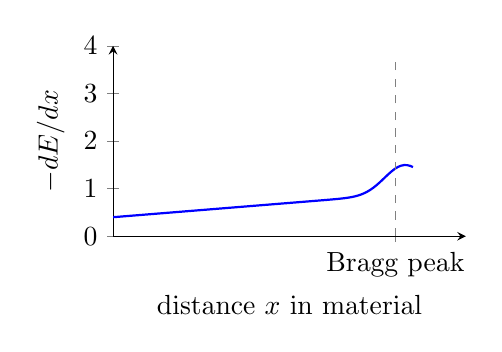
\begin{tikzpicture}
\begin{axis}[
  width=0.5\textwidth, height=4cm,
  xlabel={distance $x$ in material}, ylabel={$-dE/dx$},
  xmin=0, xmax=4, ymin=0, ymax=4,
  xtick={3.2}, xticklabels={Bragg peak},
  ytick={}, axis lines=left, samples=100,
]
  % Bragg curve: low then rapidly rising peak
  \addplot[thick,blue,domain=0:3.4]
    {0.4 + 0.15*x + 0.6*exp(-3*(x-3.3)^2/(0.3))} ;
  \draw[dashed,gray] (axis cs:3.2,0) -- (axis cs:3.2,3.8);
  \node[above,scale=0.8] at (axis cs:3.2,3.85) {stop};
\end{axis}
\end{tikzpicture}
\end{center}
\caption{Energy loss $-dE/dx$ (stopping power) as a function of depth $x$ in a material. The loss is relatively constant at first, then rises sharply to the \textbf{Bragg peak} just before the particle stops — exploited in proton therapy.}
\label{fig:bragg_peak}
\end{figure}

%%==========================================================================
\section{Central Force Potential Scattering (Recitation 15)}
%%==========================================================================

\textbf{IMPORTANT: MIGHT BE ON EXAM!}

\subsection{Setup}

\begin{figure}[H]
    \centering
    \caption{Central force scattering. The potential $U(r)$ is radially symmetric, so $\alpha_\text{left} = \alpha_\text{right}$.}
\end{figure}

\begin{itemize}
    \item Because $U(r)$ is radially symmetric, $\alpha_{\text{left}} = \alpha_{\text{right}}$.
    \item
    \[
        \frac{d\sigma}{d\Omega} = \frac{b}{\sin\theta}\left|\frac{db}{d\theta}\right|
    \]
    \item $\sigma_T \propto [\text{area}]$ --- effective cross section.
    \item Suppose:
    \[
        U = \begin{cases} \infty, & r < a \\ 0, & r > a \end{cases}
    \]
\end{itemize}

\begin{figure}[H]
    \centering
    \caption{Hard-sphere scattering geometry. The particle reflects off a hard sphere of radius $a$.}
\end{figure}

\[
    \theta = \pi - 2\phi \implies \phi = \tfrac{1}{2}(\pi - \theta)
\]
but $b = a\sin\phi = a\sin\!\left(\tfrac{1}{2}(\pi-\theta)\right) = a\cos\!\left(\tfrac{\theta}{2}\right)$.

\[
    \frac{d\sigma}{d\Omega}
    = \frac{b}{\sin\theta}\left|\frac{db}{d\theta}\right|
    = \frac{a\cos(\theta/2)}{\sin\theta}\cdot\left|-\frac{a}{2}\sin\!\left(\frac{\pi}{2}\right)\right|
    = \frac{a^2\sin(\theta/2)\cos(\theta/2)}{2\sin\theta}
    = \frac{a^2}{4}
\]

\[
    \sigma_T = \int d\sigma = \int\frac{a^2}{4}\,d\Omega
    = \iint\frac{a^2}{4}\sin\theta'\,d\theta'\,d\phi'
    = \frac{a^2}{4}\cdot 4\pi = \pi a^2,
\]
which is the ``impact area'' that the particle must hit.

\section{Central Force Potential}

\begin{enumerate}
    \item $\vect{F} = -\grad U(r) = -\dfrac{\partial U}{\partial r}\,\hat{r}$
    \item $\dfrac{d\vect{L}}{dt} = 0 \implies \vect{L} = \vect{r}\times\vect{p}$, $\vect{r}\perp\vect{L}$.
    \begin{itemize}
        \item $\mathcal{L} = \frac{1}{2}m(\dot{r}^2 + r^2\dot{\phi}^2) - U(r)$, $\phi$ is cyclic.
        \item $\implies mr^2\dot{\phi}$ is conserved.
        \item $E = K + U = \frac{1}{2}m(\dot{r}^2 + r^2\dot{\phi}^2) + U(r)$
        \[
            = \frac{1}{2}m\dot{r}^2 + \frac{mr^2\dot{\phi}^2}{2mr^2} + U(r)
            = \frac{1}{2}m\dot{r}^2 + \frac{\ell^2}{2mr^2} + U(r)
        \]
        \[
            E = \frac{1}{2}m\dot{r}^2 + U_{\text{eff}}(r)
        \]
        \[
            \dot{r} = \sqrt{\frac{2}{m}\bigl(E - U_{\text{eff}}(r)\bigr)}
        \]
        \[
            \int dr = \int\sqrt{\frac{2}{m}(E-U_{\text{eff}})}\,dt
        \]
    \end{itemize}
\end{enumerate}

\subsection{Stability of Circular Orbits}

\begin{itemize}
    \item $\dfrac{dU_{\text{eff}}}{dr} = 0$ (so you are at a local min of the potential)
    \item $\left.\dfrac{d^2 U_{\text{eff}}}{dr^2}\right|_{r=\rho} > 0$
    \item Note that $mr^2\dot{\phi} = \ell \implies \dfrac{\partial\phi}{\partial t} = \dfrac{\ell}{mr^2}$, so:
    \[
        \phi = \int\frac{\ell}{mr^2}\,dt = \int\frac{\ell}{mr^2}\,\frac{dr}{\sqrt{\dfrac{2}{m}(E-U_{\text{eff}})}}
    \]
\end{itemize}

\subsection*{Example: Conical Pendulum}

\begin{figure}[H]
    \centering
    \caption{Conical pendulum: mass $m$ on a string of length $\ell_0$ constrained to move on a cone of half-angle $\alpha$.}
\end{figure}

\[
    E = K + U = \frac{1}{2}m\dot{r}^2 + \frac{1}{2}\frac{\ell^2}{m(r\sin\alpha)^2} + mg
\]

\[
    t = \int dt = \int\sqrt{\frac{2}{m}(E-U_{\text{eff}})}\,\frac{dr}{\phantom{x}}
    = \int\frac{dr}{\sqrt{\dfrac{2}{m}\!\left(E - \dfrac{\ell^2}{2mr^2\sin^2\!\alpha} - mg\cos\alpha\right)}}
\]

\[
    \phi = \frac{\ell}{\sqrt{2m}\sin^2\!\alpha}\int\frac{dr}{r^2\sqrt{E - \dfrac{\ell^2}{2mr^2\sin^2\!\alpha} - mg\sin\alpha}}
\]

%%==========================================================================
\chapter{Principle Axes of Rotation and Rigid Body Motion}
%%==========================================================================

% Lec. 16, Wednesday January 29, 2025

\begin{itemize}
    \item Consider a 3D pendulum rotating at $\vec{\omega} = \omega\hat{z}$: in general $\vect{L} \neq I\vec{\omega}$.
\end{itemize}

\section{General Body: Inertia Tensor}

\begin{figure}[H]
    \centering
    \caption{A general rigid body rotating with $\vec{\omega} = \omega\hat{z}$. Each mass element $m_i$ is at position $\vect{r}_i$ with transverse distance $\rho_i$ from the rotation axis and axial coordinate $z_i$.}
\end{figure}

\begin{align*}
    \vect{L} &= \sum_i \vect{r}_i \times m_i\vect{v}_i
    = \sum_i m_i\,\vect{r}_i \times (\vec{\omega}\times\vect{r}_i) \\
    &= \sum_i m_i\!\left[(\vect{r}_i\cdot\vect{r}_i)\vec{\omega} - (\vect{r}_i\cdot\vec{\omega})\vect{r}_i\right]
\end{align*}

Using $r_i^2 = \rho_i^2 + z_i^2$ and $\vect{r}_i\cdot\vec{\omega} = z_i\omega$:

\[
    = \omega\sum_i m_i\!\left[(\rho_i^2 + z_i^2)\hat{z} - x_i z_i\,\hat{x} - y_i z_i\,\hat{y} - z_i^2\,\hat{z}\right]
\]

\[
    \implies \vect{L} = \omega\sum_i m_i\!\left[\rho_i^2\,\hat{z} - x_i z_i\,\hat{x} - y_i z_i\,\hat{y}\right]
\]

In general, the \textbf{inertia tensor} relates $\vect{L}$ and $\vec{\omega}$:

\[
    \begin{pmatrix} L_x \\ L_y \\ L_z \end{pmatrix}
    =
    \begin{pmatrix} I_{xx} & I_{xy} & I_{xz} \\ I_{yx} & I_{yy} & I_{yz} \\ I_{zx} & I_{zy} & I_{zz} \end{pmatrix}
    \begin{pmatrix} \omega_x \\ \omega_y \\ \omega_z \end{pmatrix}
\]

For the specific case $\omega_y = \omega_z = 0$:

\[
    \vect{L} = \begin{pmatrix} I_{xz}\,\omega \\ I_{yz}\,\omega \\ I_{zz}\,\omega \end{pmatrix}
\]

\[
    I_{zz} = \sum_i m_i\rho_i^2,\qquad
    I_{xz} = -\sum_i m_i x_i z_i = I_{zx},
    \quad\text{same for }I_{yz}\text{ but swap }x\leftrightarrow y.
\]

\textit{Example:} For two point masses A and B symmetrically placed, $I_{yz}^A = -myz$ and $I_{yz}^B = -m(-y)z$, so the off-diagonal terms cancel.

\begin{theorem}[Principal Axes]
There is a choice of axes (that does not rotate with the object) such that the inertia tensor is diagonal:
\[
    \overline{I} = \begin{pmatrix} I_1 & 0 & 0 \\ 0 & I_2 & 0 \\ 0 & 0 & I_3 \end{pmatrix}
\]
\end{theorem}

To find the principal axes: diagonalize the matrix
\[
    \begin{pmatrix} I_{xx} & I_{xy} & I_{xz} \\ I_{yx} & I_{yy} & I_{yz} \\ I_{zx} & I_{zy} & I_{zz} \end{pmatrix}
\]
The eigenvalues $\lambda_1, \lambda_2, \lambda_3$ become $I_1, I_2, I_3$.

\section{Torque and Euler's Equations}

\[
    \vect{T} = \dv{\vect{L}}{t} = \left(\dv{\vect{L}}{t}\right)_{\text{rot}} + \vec{\omega}\times\vect{L},
    \qquad \vect{v} = \vec{\omega}\times\vect{r}
\]

To see why, consider rotating the angular momentum components. After a small rotation $\Delta\theta_3$ about axis 3:

\[
    \Delta l_1 = -I_2\omega_2\,\Delta\theta_3,\quad
    \Delta l_2 = I_1\omega_1\,\Delta\theta_3,\quad
    \Delta l_3 = 0
\]

\[
    \dot{l}_1 = -I_2\omega_2\omega_3,\qquad
    \dot{l}_2 = I_1\omega_1\omega_3
    \quad\text{(think about where these appear)}
\]

\begin{formula}[Euler's Equations]
For the principal axes, $l_i = I_i\omega_i$ (directions labeled 1, 2, 3):
\[
    T_1 = I_1\dot{\omega}_1 + (I_3 - I_2)\omega_3\omega_2
\]
\[
    T_2 = I_2\dot{\omega}_2 + (I_1 - I_3)\omega_1\omega_3
\]
\[
    T_3 = I_3\dot{\omega}_3 + (I_2 - I_1)\omega_2\omega_1
\]
\end{formula}

\subsection{No Torque Situation}

Suppose $\omega_1 \gg \omega_2, \omega_3$, with $\omega_1$ constant.

\begin{enumerate}
    \item $I_1\dot{\omega}_1 = 0 \implies \omega_1 \approx \text{const}$
    \item $I_2\dot{\omega}_2 + (I_1 - I_3)\omega_1\omega_3 = 0$
    \item $I_3\dot{\omega}_3 + (I_2 - I_1)\omega_2\omega_1 = 0$
\end{enumerate}

Taking time derivatives (substituting equation 3 into the time derivative of equation 2):

\[
    I_2\ddot{\omega}_2 + (I_1-I_3)\omega_1\left(-\frac{(I_2-I_1)\omega_2\omega_1}{I_3}\right) = 0
\]

\[
    \ddot{\omega}_2 + \omega_2\omega_1^2\left[\frac{(I_1-I_3)(I_1-I_2)}{I_3 I_1}\right] = 0
    \quad\text{(const.)}
\]

If $(I_1-I_3)(I_1-I_2) > 0 \implies$ SHM with frequency:

\[
    \Omega_2 = \omega_1\sqrt{\frac{(I_1-I_3)(I_1-I_2)}{I_3 I_2}}
\]

Only if $I_1$ is max or min. If it isn't, then it isn't stable.

%%==========================================================================
\section{Rigid Body Motion (Recitation 16)}
%%==========================================================================

% Wednesday, January 29, 2025

\subsection{Angular Velocity with Euler Angles}

\begin{figure}[H]
    \centering
    \caption{Euler angles: $x,y,z$ are inertial coordinates; $x',y',z'$ are body axes. Three successive rotations: (1) rotate about $\hat{z}$ by $\phi$; (2) rotate about $\hat{x}'''$ by $\theta$; (3) rotate about $\hat{z}''$ by $\psi$.}
\end{figure}

\begin{itemize}
    \item $x,y,z \to$ inertial coordinates.
    \item $x',y',z' \to$ body axes.
    \item Rotation steps:
    \begin{enumerate}
        \item Rotate about $\hat{z}$: $\phi$
        \item Rotate about $\hat{x}'''$: $\theta$
        \item Rotate about $\hat{z}''$: $\psi$
    \end{enumerate}
    \item $\vect{r}' = U\vect{r} = U_\psi U_\theta U_\phi\,\vect{r}$ (Unitary transformation).
\end{itemize}

Rotation about 1 axis:
\[
    R_\alpha = \begin{pmatrix} \cos\alpha & \sin\alpha & 0 \\ -\sin\alpha & \cos\alpha & 0 \\ 0 & 0 & 1 \end{pmatrix}
\]

\begin{formula}[Euler Angle Transformation]
\[
    \vect{r}' =
    \begin{pmatrix} \cos\psi & \sin\psi & 0 \\ -\sin\psi & \cos\psi & 0 \\ 0 & 0 & 1 \end{pmatrix}
    \begin{pmatrix} 1 & 0 & 0 \\ 0 & \cos\theta & \sin\theta \\ 0 & -\sin\theta & \cos\theta \end{pmatrix}
    \begin{pmatrix} \cos\phi & \sin\phi & 0 \\ -\sin\phi & \cos\phi & 0 \\ 0 & 0 & 1 \end{pmatrix}
    \vect{r}
\]
\end{formula}

\[
    \vec{\omega} = \vec{\omega}_\phi + \vec{\omega}_\theta + \vec{\omega}_\psi
\]

\[
    \vec{\omega}_\phi = \dot{\phi}\,\hat{z} = U_\psi U_\theta\begin{pmatrix}0\\0\\\dot{\phi}\end{pmatrix}
    = \begin{pmatrix}\dot{\phi}\sin\theta\sin\psi \\ \dot{\phi}\sin\theta\cos\psi \\ \dot{\phi}\cos\theta\end{pmatrix}
    = \dot{\phi}(\sin\theta\sin\psi\,\hat{x}' + \sin\theta\cos\psi\,\hat{y}' + \cos\theta\,\hat{z}')
\]

\[
    \vec{\omega}_\theta = \dot{\theta}\,\hat{x}''' = U_\psi\begin{pmatrix}\dot{\theta}\\0\\0\end{pmatrix}
    = \begin{pmatrix}\dot{\theta}\cos\psi \\ -\dot{\theta}\sin\psi \\ 0\end{pmatrix}
    = \dot{\theta}(\cos\psi\,\hat{x}' - \sin\psi\,\hat{y}')
\]

\[
    \vec{\omega}_\psi = \dot{\psi}\,\hat{z}'' = \dot{\psi}\,\hat{z}'
    \quad\text{(inertial coordinates)}
\]

Thus in the body axes frame:
\[
    \vec{\omega} = \hat{x}'(\dot{\phi}\sin\theta\sin\psi + \dot{\theta}\cos\psi)
                + \hat{y}'(\dot{\phi}\sin\theta\cos\psi - \dot{\theta}\sin\psi)
                + \hat{z}'(\dot{\psi}\cos\theta + \dot{\phi})
\]

\subsection{Example: Point Mass on a Disc}

\begin{figure}[H]
    \centering
    \caption{A disc of radius $R$ and total mass $M$ (with surface mass density $\sigma = M/\pi R^2$) with a point mass $m = 3M/8$ at radius $R$ from center (point B), with the axis at point A.}
\end{figure}

\textbf{Inertia Tensor of the disc alone:}

\[
    I_{zz} = \int\sigma(x^2+y^2)\,dA = \int_0^R \sigma r^2(2\pi r\,dr) = \frac{1}{2}MR^2
\]
\[
    I_{xx} = \int\sigma y^2\,dA = \frac{1}{2}\int\sigma(x^2+y^2)\,dA = \frac{MR^2}{4}
\]
\[
    I_{yy} = \frac{MR^2}{4},\qquad I_{xy} = I_{yz} = I_{xz} = 0
\]

\[
    \implies I_{\text{disk}}^{\text{center}} = \frac{MR^2}{4}\begin{pmatrix}1&0&0\\0&1&0\\0&0&2\end{pmatrix}
\]

By the parallel axis theorem (shifting to point A):
\[
    \frac{MR^2}{4}\begin{pmatrix}1&0&0\\0&1&0\\0&0&2\end{pmatrix}
    + MR^2\begin{pmatrix}0&0&0\\0&1&0\\0&0&1\end{pmatrix}
    = \frac{MR^2}{4}\begin{pmatrix}1&0&0\\0&5&0\\0&0&6\end{pmatrix}
\]

\textbf{Inertia tensor of the point mass at B} (about A), using $I_{ab}^A = m(\delta_{ab}r^2 - r_a r_b)$:

\[
    I_{xx} = m(y^2+z^2) = mR^2,\quad
    I_{yy} = m(x^2+z^2) = mR^2,\quad
    I_{zz} = m(x^2+y^2) = 2mR^2
\]
\[
    I_{xy} = I_{yx} = -mxy = -mR^2,\quad
    I_{xz} = I_{zx} = I_{yz} = I_{zy} = 0
\]

\[
    I_{\text{point mass}}^A = \frac{3M}{8}R^2\begin{pmatrix}1&-1&0\\-1&1&0\\0&0&2\end{pmatrix}
\]

\textbf{Combined inertia tensor:}
\[
    I_{\text{combined}} = I_{\text{disk}}^A + I_{\text{point mass}}^A
    = \frac{MR^2}{8}\begin{pmatrix}13&-3&0\\-3&7&0\\0&0&18\end{pmatrix}
\]

\textbf{Finding principal axes:} Solve $I\,\vec{\xi} = \lambda\,\vec{\xi}$:

\[
    I_1 = \frac{9}{4}MR^2,\quad \vec{\xi}_1 = \begin{pmatrix}0\\0\\1\end{pmatrix} \sim \hat{z}
\]
\[
    I_2 = \frac{1}{2}MR^2 \implies \vec{\xi}_2 = \frac{1}{\sqrt{10}}\begin{pmatrix}1\\3\\0\end{pmatrix} \sim \hat{x}+3\hat{y}
\]

(Third eigenvalue $I_3$ not completed in notes.)

%%==========================================================================
\chapter{Action-Angle Variables}
%%==========================================================================

% Thursday, January 30, 2025

\section{Canonical Transformation: $q,p,h \to Q,P,H$}

\begin{itemize}
    \item Any coordinate-coordinate transformation is canonical.
    \item Consider Hamiltonians where $\pdv{h}{t} = 0$ and where $h(q,p) \to H(P)$:
    \[
        \implies \dot{P} = -\pdv{H}{Q} = 0 \implies P\text{ conserved}
    \]
    \[
        \dot{Q} = \pdv{H}{P} = \text{constant} \equiv \alpha \implies Q(t) = \alpha t + Q_0
    \]
    \item Recall generator functions $F(q,P) \equiv W(q,P)$:
    \[
        h = \frac{p^2}{2m} + U(q) = E
    \]
    \[
        p = \pm\sqrt{2m(E-U(q))}
    \]
\end{itemize}

\section{Action-Angle Principle}

\begin{figure}[H]
\begin{center}
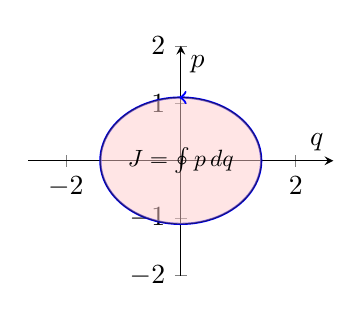
\begin{tikzpicture}
\begin{axis}[
  width=0.45\textwidth, height=4.5cm,
  xlabel={$q$}, ylabel={$p$},
  xmin=-2, xmax=2, ymin=-2, ymax=2,
  xtick={}, ytick={},
  axis lines=center, axis equal,
]
  % Closed ellipse = phase-space orbit
  \addplot[thick,blue,domain=0:360,samples=100]
    ({1.4*cos(x)}, {1.1*sin(x)});
  % Shade the interior
  \addplot[fill=red!20,opacity=0.5,domain=0:360,samples=100]
    ({1.4*cos(x)}, {1.1*sin(x)}) -- cycle;
  % Arrow on orbit
  \addplot[thick,blue,->,domain=89:91,samples=5]
    ({1.4*cos(x)}, {1.1*sin(x)});
  % Action area label
  \node[scale=0.85] at (axis cs:0,0) {$J = \oint p\,dq$};
\end{axis}
\end{tikzpicture}
\end{center}
\caption{Phase-space orbit for a bound periodic system. The trajectory is a closed curve in the $(q,p)$ plane; the enclosed area (red shading) equals the action variable $J = \oint p\,dq$, which is an adiabatic invariant.}
\label{fig:phase_space_orbit}
\end{figure}

\[
    p = \pdv{W}{q},\qquad Q = \pdv{W}{P}
    \quad\text{(comes from }F\text{)}
\]

\begin{itemize}
    \item Notice that the area (red) $= P = \oint p\,dq = \text{const}$.
    \item Let $\delta Q = \dfrac{\partial Q}{\partial q}\delta q + \dfrac{\partial Q}{\partial P}\delta P \bigg|_{\to 0}$:
    \begin{align*}
        \Delta Q\big|_{\text{1 period}}
        &= \oint\pdv{Q}{q}\,\delta q
        = \oint\frac{\partial^2 W}{\partial P\,\partial q}\,dq
        = \pdv{}{P}\oint\pdv{W}{q}\,dq \\
        &= \pdv{}{P}\oint p\,dq = 1
        \implies Q\text{ changes at a rate of 1 unit/period}
    \end{align*}
    \item Thus $\Delta Q = 1 = \alpha T$:
    \[
        \boxed{\alpha = \frac{1}{T}}
    \]
    \item But $\alpha = \pdv{H}{P} = \pdv{E}{P}$, and because energy is conserved:
    \[
        \boxed{T = \pdv{P}{E}}
    \]
\end{itemize}

\begin{formula}[Action-Angle Variables]
In action-angle formalism, $P \equiv J = \oint p\,dq$ (essentially the value of the reduced action, but for a fixed path). Then:
\[
    Q(t) = \pdv{E}{J}\,t + Q_0,\qquad Q \equiv \theta
\]
\[
    \alpha = \nu = \pdv{E}{J},\qquad T = \pdv{J}{E}
\]
\end{formula}

\subsection{Example: SHO}

\begin{figure}[H]
    \centering
    \caption{Ellipse traced by the SHO in phase space. The area $J = \pi ab$ is the action variable.}
\end{figure}

\begin{itemize}
    \item $h = \dfrac{p^2}{2m} + \dfrac{1}{2}kx^2 = E$
    \item In phase space: $\dfrac{x^2}{a^2} + \dfrac{p^2}{b^2} = 1$
    \item We know that $J = \text{area} = \pi ab$:
    \[
        = \pi\sqrt{2mE}\cdot\sqrt{\frac{2E}{k}} = 2\pi E\sqrt{\frac{m}{k}}
    \]
    \item $T = \pdv{J}{E} = 2\pi\sqrt{\dfrac{m}{k}} = \dfrac{2\pi}{\omega}$
    \item To find $Q$: $\phi(t) = 2\pi\cdot\dfrac{\omega}{2\pi} = \omega t$
\end{itemize}

\subsection{Cycloid Problem}

\begin{figure}[H]
    \centering
    \caption{Shape of the well formed by a cycloid (parametrized by $\phi$). The potential is zero at the top of the cycloid.}
\end{figure}

\begin{itemize}
    \item $X(\phi) = R(\phi + \sin\phi)$, $Y(\phi) = -R\cos\phi$
    \item Start at $\phi(0) = \phi_0$, $\dot{\phi}(0) = 0$; how long does it take to get to the bottom?
\end{itemize}

\[
    \dot{X} = R(\dot{\phi} + \cos\phi\,\dot{\phi}),\quad \dot{Y} = R\sin\phi\,\dot{\phi}
\]
\[
    V^2 = \dot{X}^2 + \dot{Y}^2 = R^2\dot{\phi}^2(1 + \cos^2\phi + 2\cos\phi + \sin^2\phi)
    = 2R^2\dot{\phi}^2(1+\cos\phi)
\]

\[
    L = mR^2\dot{\phi}^2(1+\cos\phi) + mgR(\cos\phi - 1)
\]
\[
    = mR^2\dot{\phi}^2\cdot 2\cos^2\frac{\phi}{2} - mgR\cdot 2\sin^2\frac{\phi}{2}
    = 2mR^2\dot{\phi}^2\cos^2\frac{\phi}{2} - 2mgR\sin^2\frac{\phi}{2}
\]

\[
    p = \pdv{L}{\dot{\phi}} = 4mR^2\dot{\phi}\cos^2\frac{\phi}{2}
\]

Notice that $p\dot{\phi} = 2K$.

\[
    H = p\dot{\phi} - L = 2mR^2\cos\frac{\phi}{2}\cdot\frac{p^2}{\underbrace{16m^2R^4\cos^4(\phi/2)}} + 2mgR\sin^2\frac{\phi}{2} = E
\]
\[
    = \frac{p^2}{8mR^2\cos^2\!\frac{\phi}{2}} + 2mgR\sin^2\frac{\phi}{2} = 2mgR\sin^2\frac{\phi}{2}
\]

\[
    \implies p^2 = 8mR^2\cos^2\frac{\phi}{2}\left[2mgR\!\left(\sin^2\frac{\phi_0}{2} - \sin^2\frac{\phi}{2}\right)\right]
\]

\[
    J = \oint p\,d\phi = 4\int_0^{\phi_0} p\,d\phi
    = 16mR^{3/2}\sqrt{g}\int_0^{\phi_0}d\phi\cos\frac{\phi}{2}\sqrt{\sin^2\frac{\phi_0}{2} - \sin^2\frac{\phi}{2}}
\]

(Make sure the integral is positive.)

Substitution: $z = \sin\dfrac{\phi}{2}$, $dz = \cos\dfrac{\phi}{2}\dfrac{d\phi}{2}$, $z_0 = \sin\dfrac{\phi_0}{2}$:

\[
    J = 16mR^{3/2}\sqrt{g}\int_0^{z_0} 2\,dz\sqrt{z_0^2 - z^2}
\]

\[
    = 16mR^{3/2}\sqrt{g}\left[z_0^2\sin^{-1}\!\left(\frac{z}{z_0}\right) + z\sqrt{z_0^2-z^2}\right]_0^{z_0}
    = z_0^2\frac{\pi}{2} - 0 - 0
    = \frac{\pi}{2}\sin^2\frac{\phi_0}{2}
\]

\[
    J = 16mR^{3/2}\sqrt{g}\cdot\frac{\pi E}{4mgR} = 4\pi E\sqrt{\frac{R}{g}}
\]

\[
    T = \pdv{J}{E} = 4\pi\sqrt{\frac{R}{g}} \implies \boxed{\text{time to bottom is }\pi\sqrt{\frac{R}{g}}}
\]

%%==========================================================================
\chapter{Final Summary}
%%==========================================================================

% Thursday, January 30, 2025

\section{Constrained Motion}

\section{Final Exam Review (Recitation 17)}

\[
    \mathcal{L}(q,\dot{q},t) = K(\dot{q},t) - U(q,t)
\]

\textbf{EOM:}
\[
    \dv{t}\!\left(\pdv{\mathcal{L}}{\dot{q}}\right) - \pdv{\mathcal{L}}{q} = 0
\]

\subsection{If Constraints:}

\subsubsection{(1) Holonomic Constraints}

No $\dot{q}$ dependence $\implies f_\alpha^{\text{index of constraint}}(\vec{q}, t) = 0$.

E.g.\ motion restricted to specific surfaces:
\[
    r^2 - (x^2 + y^2) = 0\quad\text{(cone)}
\]

\begin{formula}[Generalized Forces]
\[
    F_\alpha(\vec{q},t) = \lambda_\alpha\,\pdv{f_\alpha}{q_a}
\]
\end{formula}

\[
    \dv{t}\!\left(\pdv{\mathcal{L}}{\dot{q}_i}\right) - \pdv{\mathcal{L}}{q_i}
    = \sum_\alpha \lambda_\alpha\,\pdv{f_\alpha}{q_i}
\]

\subsubsection{(2) Semi-Holonomic}

Linear dependence on $\dot{q}$:

\begin{formula}[Semi-Holonomic Constraint]
\[
    f = \sum_i a_i(q_i, t)\,\dot{q}_i + B(q_i, t) = 0
\]
\[
    f = \dv{t}\!\bigl(g(q_i,t)\bigr),\quad\text{where }a_i = \pdv{g}{q_i},\quad B = \pdv{g}{t}
\]
\end{formula}

\textbf{Conditions:} Because $\dfrac{\partial g}{\partial q_i\,\partial t} = \dfrac{\partial^2 g}{\partial t\,\partial q_i}$:
\begin{enumerate}
    \item $\pdv{a_i}{t} = \pdv{B}{q_i}$
    \item $\pdv{a_i}{q_j} = \pdv{a_j}{q_i}$
\end{enumerate}

\[
    \text{EOM:}\quad\dv{t}\!\left(\pdv{\mathcal{L}}{\dot{q}_i}\right) - \pdv{\mathcal{L}}{q_i}
    = \sum_\alpha \lambda_\alpha\,\partial f_\alpha
\]

\subsection{Hamiltonian}

\textit{Last-minute question: when is the Hamiltonian $=$ energy $= K+U$?}

\begin{formula}[Hamiltonian]
\[
    H(q,p,t) = \sum_i p_i\dot{q}_i - \mathcal{L}(q,\dot{q},t),\quad\text{where }p_i \equiv \pdv{\mathcal{L}}{\dot{q}_i}
\]
\end{formula}

\textbf{EOM:}
\[
    \pdv{H}{p_i} = \dot{q}_i,\qquad
    \pdv{H}{q_i} = -\dot{p}_i,\qquad
    \pdv{H}{t} = -\pdv{\mathcal{L}}{t}
\]

In order for $H = E$, there must be no explicit time dependence.

\subsection{Non-Hamiltonian Forces}

They can be added as such:
\[
    \dot{p}_i = -\pdv{H}{q_i} + F_i
\]

\subsection{Poisson Brackets}

\[
    [f,g] = \sum_k\left(\pdv{f}{q_k}\pdv{g}{p_k} - \pdv{f}{p_k}\pdv{g}{q_k}\right)
\]

Check if a quantity is conserved:
\begin{formula}[Time Evolution via Poisson Bracket]
\[
    \boxed{\dv{f}{t} = \pdv{f}{t} + [f, H]}
\]
\end{formula}

\subsubsection{Canonical Coordinate Transformation Requirements}

To show that $q\to Q$, $p\to P$ is canonical, you need to show that $[Q_i, Q_k]_{q,p}$, $[Q_i, Q_i]_{q,p}$, $[P_i, P_k]_{q,p}$ satisfies (1), (2), (3):

\begin{enumerate}
    \item $[q_i, q_k] = 0$
    \item $[p_i, p_k] = 0$
    \item $[q_i, p_k] = \delta_{ik}$
\end{enumerate}

\subsubsection{Useful Identities}

\begin{enumerate}
    \item $[q_i, q_j]_{q,p} = [p_i, p_j]_{q,p} = 0$
    \item $[q_i, p_j]_{q,p} = \delta_{ij}$
    \item $[F, G] = -[G, F]$
\end{enumerate}

With the Hamiltonian:
\begin{enumerate}
    \item $[q, H] = \dot{q}$
    \item $[p, H] = \dot{p}$
\end{enumerate}

\begin{fact}[Conservation via Poisson Brackets]
If $[F,H] = [G,H] = 0$ (i.e., $F$ and $G$ are conserved), then $[F,G]$ is also conserved.

\textit{Example:} Angular momentum can only be conserved for 1 or 3 axes.
\end{fact}

\begin{formula}[Poisson Brackets Invariant Under Canonical Transformations]
\[
    [F,G]_{p,q} = [F,G]_{P,Q}
\]
\end{formula}

\section{Generating Canonical Transformations}

We want to find a function $F(q,P,t)$ such that:
\begin{formula}[Generator Function]
\[
    \boxed{p = \pdv{F}{q},\qquad Q = \pdv{F}{P},\qquad H = h + \pdv{F}{t}}
\]
\end{formula}

\begin{enumerate}
    \item Find the transformed Hamiltonian $H$.
    \item Find the equations of motion and solve.
    \item Transform back to original coordinates $q,p$.
\end{enumerate}

\section{Infinitesimal Canonical Transformations}

For $F$'s of the form $F = qP + \varepsilon f(q,P)$ for $\varepsilon$ small:
\[
    p = \pdv{F}{q},\qquad Q = \pdv{F}{P}\quad\text{as usual}
\]

But now:
\begin{enumerate}
    \item If $f(q,p) = h(q,p) \implies$ \textbf{Hamiltonian generates time-translation!}
    \begin{itemize}
        \item e.g.\ $p = p(t+\delta t)$, $Q = q(t+\delta t)$ (regardless of whether $E$ is conserved).
    \end{itemize}
    \item If $F(q,p) = qP + \delta q\,p \implies$ \textbf{Momentum is always the generator of space translation!}
    \item \textbf{Angular momentum is the generator of rotations!}
\end{enumerate}

\section{Liouville's Theorem}

\begin{itemize}
    \item Continuity equation: $\pdv{\varrho}{t} + \grad\cdot\vect{J} = 0$
    \item The density of states in an ensemble of identical states with different initial conditions is constant along every trajectory in phase space, NOT at any fixed point $\left(\pdv{\varrho}{t} = 0\right)$.
    \item \textbf{Important:} For a non-Hamiltonian force $F$, the Liouville equation becomes:
    \[
        \pdv{\varrho}{t} + \sum_i\pdv{F_i}{p_i}\,\varrho = 0
    \]
    \item If $F$ is divergence-free with respect to momentum space $\left(\sum_i\pdv{F_i}{p_i} = 0\right)$, then $\pdv{\varrho}{t} = 0$.
    \item Canonical transformations preserve phase space volumes!
\end{itemize}

%%==========================================================================
\section{Scattering (Summary)}
%%==========================================================================

\begin{figure}[H]
    \centering
    \caption{Scattering summary diagram. A particle with initial momentum $\vect{p}_i$ and impact parameter $b$ scatters off a potential centered at the origin through angle $\theta$. The solid angle element $d\Omega$ subtended by the scattered ring is shown.}
\end{figure}

\begin{itemize}
    \item $\theta$ (scatter angle): direction between initial and final $\vect{p}$.
    \item $b$: impact parameter, $b = R\sin\alpha$.
    \item $\alpha$: angle from origin to point of closest approach.
    \item \textbf{Important:} If the potential has azimuthal symmetry, the trajectory of the particle obeys time-translation symmetry $\implies$
    \[
        \boxed{\theta = \pi - 2\alpha}
    \]
\end{itemize}

\subsection{Differential Cross Section}

\[
    \int\frac{d\sigma}{d\Omega}\,d\Omega = \sigma_T \propto [\text{area}]
    = \frac{\text{total scattering rate}}{L}
    \quad\left(\frac{\#\text{ particles}}{\text{[time][area]}}\right)
\]

\[
    \implies \left(\frac{d\sigma}{d\Omega}\right)\Delta\Omega\text{ is scattering rate through }\Delta\Omega\text{ divided by }L
\]

\[
    d\Omega = \sin\theta'\,d\theta'\,d\phi = 2\pi\sin\theta'\,d\theta'
    \implies \int d\Omega = 4\pi
\]

If $b(\theta)$ is 1-to-1, then the rate of beam particles in $[b,\Delta b]$ equals the rate of particles scattering through $d\Omega$:

\begin{formula}[Differential Cross Section]
\[
    \boxed{\frac{d\sigma}{d\Omega} = \frac{b}{\sin\theta}\left|\frac{db}{d\theta}\right|}
\]
\end{formula}

\subsection{Calculating Mean Free Path}

\begin{itemize}
    \item Enter rest frame of the particle.
    \item Suppose potential wells have a density of $\rho_U$.
    \item Suppose beam velocity is $v_n$.
    \item The luminosity of the beam is $= \rho v_n$.
    \item Thus the mean free path:
    \[
        D = \frac{v_n}{L\sigma} = \frac{v_n}{\rho\,v_n} = \frac{1}{\rho\,\sigma}
    \]
\end{itemize}

\subsection{Handy Formula: Central Potential}

If $U$ is a central potential, angular momentum is conserved:
\[
    E = \frac{1}{2}m\dot{r}^2 + \frac{\ell^2}{2mr^2} + U(r),\qquad
    \ell^2 = (bp_0)^2 = b^2\cdot 2mE_0
\]

Circular orbit is stable when $\dfrac{dU_{\text{eff}}}{dr} = 0$ and $\left.\dfrac{d^2U_{\text{eff}}}{dr^2}\right|_{r=\rho} > 0$.

\section{Rigid-Body Motion (Summary)}

\begin{itemize}
    \item There is a choice of axes such that the inertia tensor is diagonal.
    \item If $\omega_1 \gg \omega_2, \omega_3$, the rotation is only stable if $I_1$ is a \underline{minimum} or \underline{maximum}.
    \item Frequency for SHM:
    \[
        \Omega_2 = \omega_1\sqrt{\frac{(I_1-I_3)(I_1-I_2)}{I_3 I_2}}
    \]
\end{itemize}

%%==========================================================================
\section{Examples}
%%==========================================================================

\subsection{Canonical Transformation Example}

\begin{example}[Verifying Canonical Transformation]
Let $Q = p + iaq$, $P = \dfrac{p - iaq}{2ia}$.

Want to show (WTS) $[Q,Q]_{q,p} = 0$:
\[
    [Q,Q] = \pdv{Q}{q}\pdv{Q}{p} - \pdv{Q}{p}\pdv{Q}{q} = 0
\]
$[P,P]_{q,p} = 0$: same as above.

$[Q,P] = 1$:
\[
    [Q_1, P] = \pdv{Q}{q}\pdv{P}{p} - \pdv{Q}{p}\pdv{P}{q}
    = ia\cdot\frac{1}{2ia} - 1\cdot\left(-\frac{ia}{2ia}\right)
    = \frac{1}{2} + \frac{1}{2} = 1\checkmark
\]
\end{example}

\subsection{Constraints Example: Hoop Rolling on a Cylinder}

\begin{figure}[H]
    \centering
    \caption{A hoop of mass $m$ and radius $r$ rolling without slipping on a cylinder of radius $R$. The hoop starts from rest on top of the cylinder.}
\end{figure}

\begin{itemize}
    \item Hoop rolls without slipping on the cylinder.
    \item Starts from rest on top of the cylinder.
    \item Rolling without slipping --- write ALL constraints!
    \[
        g_1 = \dot{\rho} = 0,\quad \rho = R + r\quad\text{(semi-holonomic)}
    \]
    \[
        g_2 = \rho\dot{\theta} - r\dot{\phi} = 0
    \]
\end{itemize}

\[
    L = \frac{m}{2}(\dot{\rho}^2 + \rho^2\dot{\theta}^2) + \frac{m}{2}r^2\dot{\phi}^2 - mg\rho\cos\theta
    \quad (I_{\text{hoop}} = mr^2)
\]

Equations of motion with generalized forces:

\begin{align*}
    \rho:&\quad\dv{t}\!\left(\pdv{L}{\dot{\rho}}\right) - \pdv{L}{\rho} - \sum_i\lambda_i\pdv{g_i}{\dot{\rho}} = 0\\
    &\implies m\ddot{\rho} - m\rho\dot{\theta}^2 + mg\cos\theta - \lambda_1 = 0\\[6pt]
    \theta:&\quad\dv{t}\!\left(\pdv{L}{\dot{\theta}}\right) - \pdv{L}{\theta} - \sum_i\lambda_i\pdv{g_i}{\dot{\theta}} = 0\\
    &\implies \dv{t}(m\rho^2\dot{\theta}) - mg\rho\sin\theta - \lambda_2\rho = 0\\[6pt]
    \phi:&\quad\dv{t}\!\left(\pdv{L}{\dot{\phi}}\right) - \pdv{L}{\phi} - \sum_i\lambda_i\pdv{g_i}{\dot{\phi}} = 0\\
    &\implies mr^2\ddot{\phi} + \lambda_2 r = 0
\end{align*}

\[
    F_\rho = \sum_i\lambda_i\pdv{g_i}{\dot{\rho}} = \lambda_1 = 0
    \implies \text{no force on the contact point}
\]

From the $\phi$ equation: $\lambda_2 = -mr\ddot{\phi} = -mr\ddot{\theta}$ (since $\rho\dot{\theta} = r\dot{\phi}$ implies $\dot{\phi} = \dot{\theta}$ for $\rho = R+r \approx R$).

From the $\theta$ equation:
\[
    \dv{t}(m\rho^2\dot{\theta}) - mg\rho\sin\theta - \rho\lambda_2 = 0
\]
\[
    2m\rho\dot{\rho}\dot{\theta} + m\rho^2\ddot{\theta} - mg\rho\sin\theta - \rho\lambda_2 = 0
\]

Since $\dot{\rho} = 0$:
\[
    \implies \boxed{\ddot{\theta} = \frac{g\sin\theta}{2\rho}}
\]

Solve this to get $\dot{\theta}^2 = \dfrac{g}{\rho}(1 - \cos\theta)$.

Plug into EOM for $\rho$ to get $\ddot{\rho} = 0$:
\[
    \lambda_1 = mg(2\cos\theta - 1) = 0 \implies \boxed{\theta = \frac{\pi}{3}}
\]


\end{document}




